\chapter{SBN Oscillation Analysis Within the VALOR Framework}
\label{chap:VALOR}

The VALOR framework is a neutrino fitting framework that was first developed for the \gls{t2k} experiment but has since been adapted to also cover Hyper-Kamiokande, \gls{dune} and the \gls{sbn} program \cite{VALOR}.

Performing an analysis within VALOR involves a number of physics parameters that define a physics hypothesis (e.g. neutrino oscillations) and the relevant systematic uncertainties. Event rate predictions are constructed for the associated detector, beam and event sample. These predictions are constructed as a function of a kinematical variable for either a nominal scenario or with variations due to a physics hypothesis and/or systematic uncertainties. This approach allows for joint oscillation and systematic fits to be constructed from a binned likelihood fitting approach for a given event topology. Fits may be performed for individual detectors or for a combination of multiple detectors and may include any number of systematic uncertainties. 

\section{The VALOR Framework}\label{sec:VALOR_framework}

The data inputs used for an oscillation analysis are mainly provided in the form of \glspl{mct}, which provide a mapping between true and reconstructed variables. They are constructed following the full event processing chain which includes event simulation, reconstruction and selection. Since the \glspl{mct} include the effects from reconstruction and selection, it is not feasible to directly recreate them using only information on the flux, cross-section and efficiency. These \glspl{mct}, \textit{T}, encapsulate a number of quantities describing a given event and are listed below,

\begin{itemize}
    \item[b] -- Beam configuration e.g. neutrino or anti-neutrino mode,
    \item[d] -- Detector e.g. \gls{sbnd}, \gls{microboone} or \gls{icarus},
    \item[s] -- Topological event selection e.g. \nue \gls{cc}-inclusive, \numu \gls{cc}-inclusive,
    \item[m] -- True Reaction Mode e.g. \numu~\gls{cc} QE, \nue~\gls{cc} 1$\pi^{\pm}$,
    \item[r] -- A bin in multi-dimensional reconstructed kinematic space e.g. $E_{\nu, reco}$,
    \item[t] -- A bin in multi-dimensional true kinematic space e.g. $E_{\nu, true}$,
\end{itemize}

with $T = T_{d;b;s;m}(r, t)$. By combining \textit{T} with the necessary physics parameters, $\vec{\theta}$, and systematic parameters, $\vec{f}$, the predicted event rate, $n^{pred}_{d;b;s}$, may be expressed as
\begin{equation}
n_{d;b;s}^{pred}(r; \vec{\theta}; \vec{f}) =
   \sum_{m} \sum_{t}  P_{d;b;m}(t; \vec{\theta}) \cdot R_{d;b;s;m}(r,t; \vec{f}) \cdot T_{d;b;s;m}(r,t) \cdot N^{MC},
   \label{eq:valor_npred}
\end{equation}
where $P_{d;b;m}(t; \vec{\theta})$ represents the effect due to a physics hypothesis, $R_{d;b;s;m}(r,t; \vec{f})$ represents the response of a \gls{mct} bin to the systematic variations and $N^{MC} = \mbox{POT}_{b;d}^{data}/\mbox{POT}_{b;d}^{MC}$, which is the normalisation by which to scale the event rate to account for the POT which was used to construct the sample of neutrino events with respect to the nominal POT in the analysis. The variation due to systematic parameters is applied separately to each combination of beam, detector, topological selection and reaction mode in true-reconstructed space and is, therefore, dependant on, \textit{b, d, s} and \textit{m}. The dependence of $P_{d;b;m}(t; \vec{\theta})$ on \textit{d} and \textit{b} is due to \textit{d} and \textit{b} encapsulating the baseline information which is a component of the oscillation probability. The unoscillated \gls{cc} \glspl{mct} are weighted by the appropriate oscillation probability, $P_{\nu_{\alpha} \rightarrow \nu_{\beta}}$, to reflect the change in event rate due to neutrino oscillations. The \gls{nc} \glspl{mct} are left unweighted since they remain unchanged due to flavour oscillations. This distinction between \gls{cc} and \gls{nc} is encapsulated by \textit{m}, hence, $P_{d;b;m}(t; \vec{\theta})$ is required to also be dependent on \textit{m}. 

For $n_{d ; b ; s}^{obs}(r)$ observed events, the log likelihood, $\lnOf{\lambda_{d;b;s}(\vec \theta, \vec f)}$, is given by
\begin{equation}
    \lnOf{\lambda_{d;b;s}(\vec \theta, \vec f)} = - \mathlarger{\mathlarger{\sum_{b,d,s,r}}} \Bigg \{ \Big (n_{d;b;s}^{pred}(r,\vec{\theta},\vec{f})
    - n_{d ; b ; s}^{obs}(r) \Big) + n_{d ; b ; s}^{obs}(r) \cdot \lnOf{\frac{n_{d ; b ; s}^{obs}(r)}{n_{d ; b ; s}^{p r e d}(r , \vec{\theta} , \vec{f})}} \Bigg \}.
\end{equation}
An additional term is applied to penalise deviations from the nominal values of systematic parameters which is defined as,
\begin{equation}
    \lnOf{\lambda_{syst}(\vec{f})} = -\frac{1}{2} (\vec{f} - \vec{f}_0)^T \mathbf{V^{-1}} (\vec{f} - \vec{f}_0),
\end{equation}
where $\vec{f}_0$ is a vector containing the nominal value of all the systematic parameters and \textbf{V} is a covariance matrix containing the uncertainties of the systematic parameters \cite{VALOR_dune}. 

In the limit of large statistics, quantities of the form $-2\lnOf{\lambda}$ have a $\chi^2$ distribution, hence calculating the log-likelihood allows a goodness-of-fit test to be performed \cite{introduction_to_mathematical_statistics_book}. The total goodness-of-fit value is therefore given by,
\begin{equation}
    \chi^2_{tot} = -2(\lnOf{\lambda_{d;b;s}(\vec{\theta}, \vec{f})} + \lnOf{\lambda_{syst}(\vec{f})}).
\end{equation}

In order to create confidence regions, fits are performed between a certain \textit{Asimov} dataset and $n_{d;b;s}^{pred}$. The Asimov dataset is a dataset where all systematic parameters are set to their nominal values and serves as a proxy for data in cases where only simulations are considered. It has been shown that in the same limit as the $\chi^2$ approximation (in the limit of large statistics), the median of many toy \gls{mc} experiments is equivalent to the Asimov dataset. This allows the significance of a given hypothesis to be compared to the median one whilst only requiring one \textit{toy} experiment instead of needing to compute many toy \gls{mc} experiments \cite{Asimov_dataset}. Two types of confidence regions may be constructed; an \textit{exclusion} region and an \textit{allowed} region. Both regions show the area where the chosen model is either compatible or incompatible with the data. The difference is due to the input data which has either no oscillation signal (an exclusion region) or there is an injected signal (an allowed region). In the case of exclusion regions, the Asimov dataset corresponds to the case where no oscillations are observed which is the null-hypothesis and for allowed regions, the oscillation parameters are set to that of the injected signal. %For the \glspl{mct}, the oscillation parameters are set to a given value and the systematic parameters, if any, are allowed to float.

\section{Oscillation Channels Within SBN}

As was discussed in \SectionRef{sec:sbn_physics_capabilities}, the \gls{bnb} is \numu dominated with a small portion of \nue's present. In the presence of mixing with a light sterile neutrino 
this would result in the disappearance of some percentage of the \numu's due to oscillations. Additionally, \numu to \nue oscillations via sterile neutrinos would result in the increase of the number of \nue's present. Finally, the number of intrinsic \nue's present in the \gls{bnb} coupled with the large event rate \gls{sbn} will detect means there are sufficient statistics to observe the disappearance of some \nue's due to oscillations. This results in three possible oscillation channels, \numu disappearance, \nue appearance and \nue disappearance. The mixing angles which determine their respective oscillation probabilities are shown in Equations (\ref{eqn:sinsq2thmumu} -- \ref{eqn:sinsq2thee}) which also imply that the oscillation channels are coupled (that is the presence of non-zero \nue appearance also requires non-zero \numu disappearance and \nue disappearance). Despite this, currently, the oscillation channels are treated completely independently. In principle oscillations involving \nutau are also possible, but due to the high energy threshold required these are usually not expected to be observed with any significant statistics. The energy range of the \gls{bnb} above the \nutau threshold is of the order 1\%, but since the statistics in \gls{sbnd} are large, this may be sufficient to observe \numu to \nutau appearance. Currently, this channel is not considered in the analysis but may be explored in future work \cite{tau_oscillations}.

The \numu disappearance as well as both the \nue channels have already been explored by a number of different experiments, many of which have been discussed in \SectionRef{subchap:Motivation for Sterile Neutrinos}. This has led to tension due to the conflict between null-results from some experiments and the hints of possible mixing with light sterile neutrinos seen by others. \gls{sbn} will be particularly sensitive to the \numu disappearance and \nue appearance channels due to the high flux of \numu's observed which will allow for the \gls{lsnd} and \gls{miniboone} anomalies to be investigated. Additionally, \gls{sbn} will be simultaneously sensitive to \numu disappearance and \nue appearance. 

\begin{comment}
    
The \numu disappearance channel has for example been investigated by \gls{minos}/\gls{minos}+, \gls{miniboone}/\gls{sciboone} and the IceCube experiment. The combined results from the \gls{miniboone} and \gls{sciboone} collaborations and a \gls{miniboone} only analysis (along with other experimental results) are shown on the left of \FigureRef{fig:miniboone_sciboone_minos}. The exclusion contours from \gls{minos} and \gls{minos}+ are shown on the right of \FigureRef{fig:miniboone_sciboone_minos}, with the black line representing the data and the dashed blue line being the expected sensitivity \cite{MiniBooNE/SciBooNE_numu_disapp_contour} \cite{MINOS_numu_disapp_contour}. It should be noted that the results from \gls{minos} are shown as a function of $\sin^2{\theta}$ instead of $\sin^2{2\theta}$ which is used for most other results. The results from 8 years of IceCube data are shown in \FigureRef{fig:icecube} along with other experimental results. The left plot is the 90\% C.L. allowed region, whereas the right plot is the 99\% C.L. exclusion contour. The star in each plot represents the best-fit point. The results depend on both $\theta_{24}$ and $\theta_{34}$, but the contours have been produced under the assumption that $\theta_{34} = 0$ \cite{IceCube_numu_disapp_contour}.

For the \nue appearance channel, the allowed regions from the \gls{lsnd} and \gls{miniboone} experiments are shown on the left of \FigureRef{fig:allowed_exclusion_region_tension}, along with exclusion contours from experiments including, \gls{icarus}, \gls{karmen}, NOMAD, OPERA and E776 (which is combined with solar neutrino data)\cite{LSND_excess}\cite{MiniBooNE_nue_app_contour}\cite{icarus_nue_app_contour}\cite{KARMEN_nue_app_contour}\cite{NOMAD}\cite{OPERA}\cite{E776}. The \gls{lsnd} result are produced from a combination of neutrinos from decay at rest (DaR) $\pi^+$ as well as decay in flight (DiF) pions meaning appearance of both \nue and \nuebar are considered. \gls{miniboone} also observed both neutrino and antineutrinos from the \gls{bnb}, whereas the \gls{karmen} experiment considered the oscillations of \numubar exclusively and the remaining experiments mentioned considered the oscillations of \numu exclusively \cite{LSND_KARMEN_nue_app_contour}.

Finally, the \nue disappearance channel has been investigated with allowed regions being obtained from gallium and reactor experiments and exclusion regions being obtained from \nue-carbon interaction data and solar neutrino data. Additionally, the near detector of the \gls{t2k} experiment has provided both allowed and excluded regions which are shown in the left plot of \FigureRef{fig:nue_disapp_external}. An overlay of the \gls{t2k} exclusion region along with the other experimental results are shown in the right plot of \FigureRef{fig:nue_disapp_external}, all of which are shown at the 95\% CL. In both cases, the coloured star and circles correspond to the best-fit point of a given result \cite{T2K_nue_disapp_contour}. 

\end{comment}
The remainder of this chapter will focus on the \nue channels. Some of the key results for the \numu channel are shown in \AppendixRef{app:numu_disapp} and a detailed discussion can be found in \cite{Rhiannon's_thesis}.

\section{Specifics of SBN Sensitivity Simulation Implementation in VALOR}

\subsection{Baseline and Binning Analysis Choices}

Two other key analysis choices are the neutrino baseline parameterisation and the binning scheme used for the kinematic variable. As is shown in \EquationRef{eqn:sterile_osc_prob}, the baseline is one of the components that drives the oscillation probability and therefore any approximations to the true baseline must be chosen such that the impact to the oscillation probability is negligible. The kinematic variable used in this analysis is the energy of the neutrino for both true and reconstructed quantities.

\subsubsection{Baseline}
For long baseline experiments, it is not uncommon for fitting frameworks to simply use some average value for the baseline since factors such as the interaction point in the detector or the position at which a particle decays into a neutrino would only change the average baseline for the experiment by a negligible amount. However, for short baseline experiments such as \gls{sbn}, these factors may change the baseline significantly, up to around 20\% in \gls{sbnd}. 

In an attempt to minimise computing resources, the true baseline was not initially used, but instead, several approximations to the baseline were tried. To begin with, the average baseline of each \gls{sbn} detector was used for all neutrino energies. This was calculated from the true baseline distribution of \numu events in each detector which are shown in \FigureRef{fig:numu_baseline}. Secondly, a 4-knot spline (named spline V1) for each detector was defined in order to try and better approximate the baseline. This method was improved upon by producing a spline for each of the true energy bins (named spline V2) which are defined in \SectionRef{sec:binning}. In order to establish the impact of any baseline approximations on the oscillation probability, the oscillation probability was plotted as a function of true neutrino energy with the oscillation parameters $\sin^2{2\theta_{\mu\mu}} = 0.01$ and $\Delta m^2_{41} = 50$ eV$^2$. This oscillation point was chosen to ensure that a region where rapid oscillations occur was being investigated, which would highlight the effect of any baseline choices. The oscillation probabilities as a function of energy are shown in \FigureRef{fig:baseline_osc_probability} for the four different baselines described. It was eventually decided that any approximation would be insufficient and that the true baseline should be used. 

\begin{figure}[h!]
	\centering
	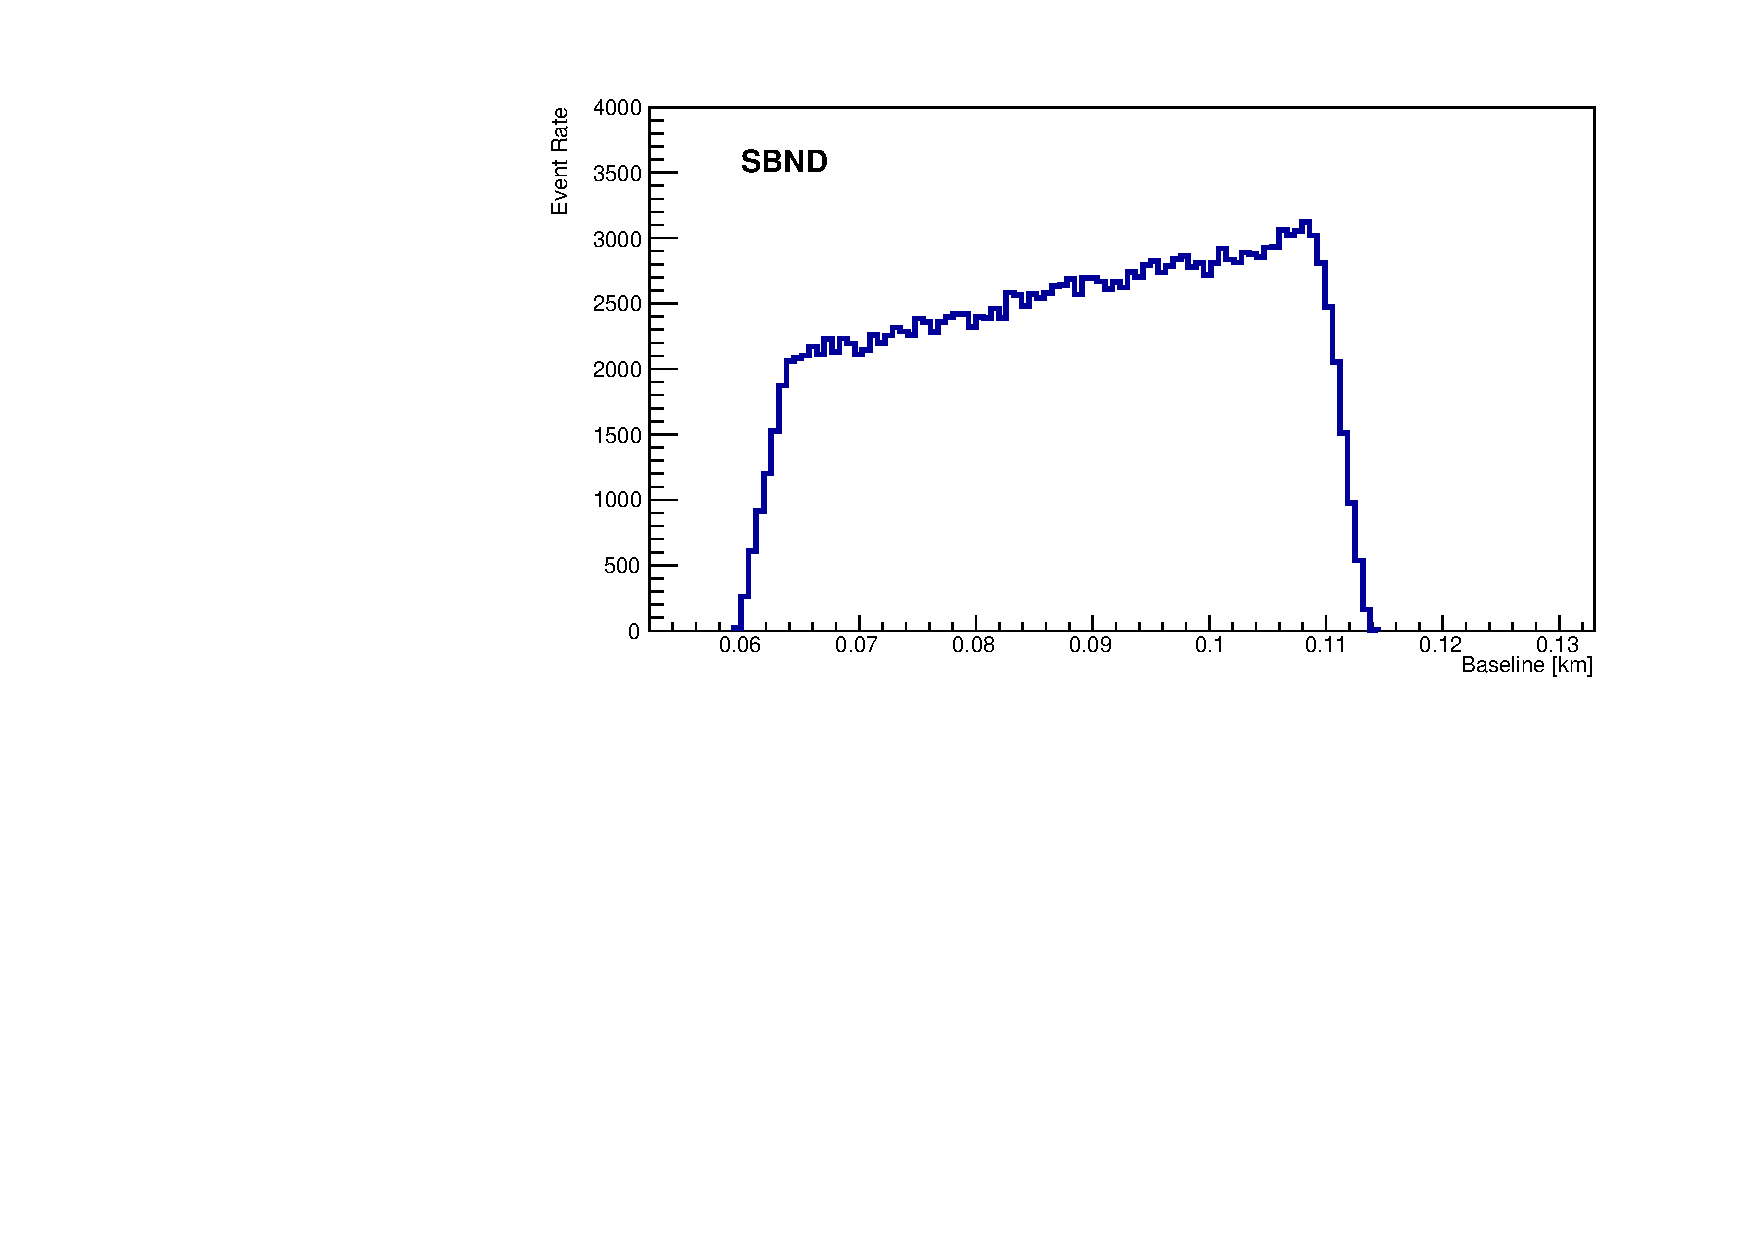
\includegraphics[width = 0.49\textwidth]{figures-chap5/SBND_numu.pdf}
	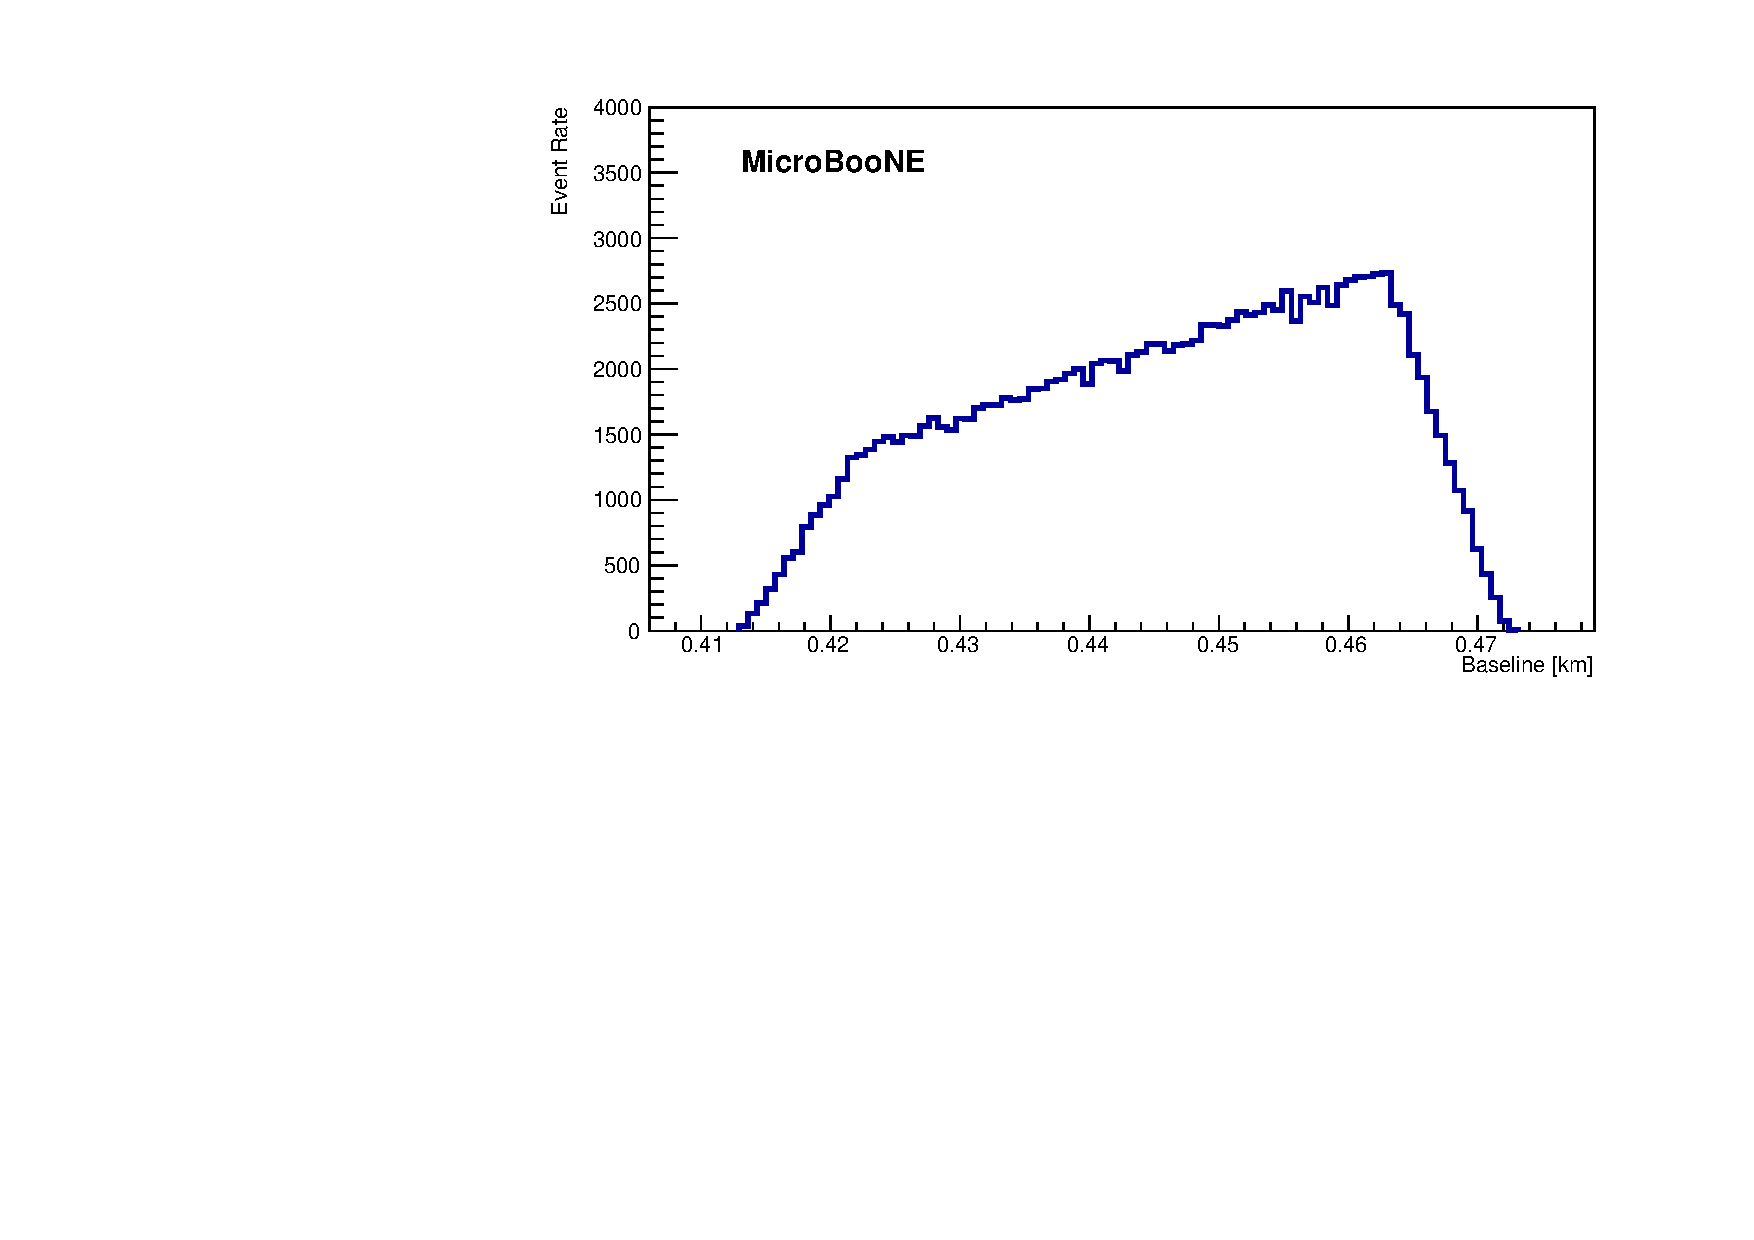
\includegraphics[width = 0.49\textwidth]{figures-chap5/MicroBooNE_numu.pdf}
	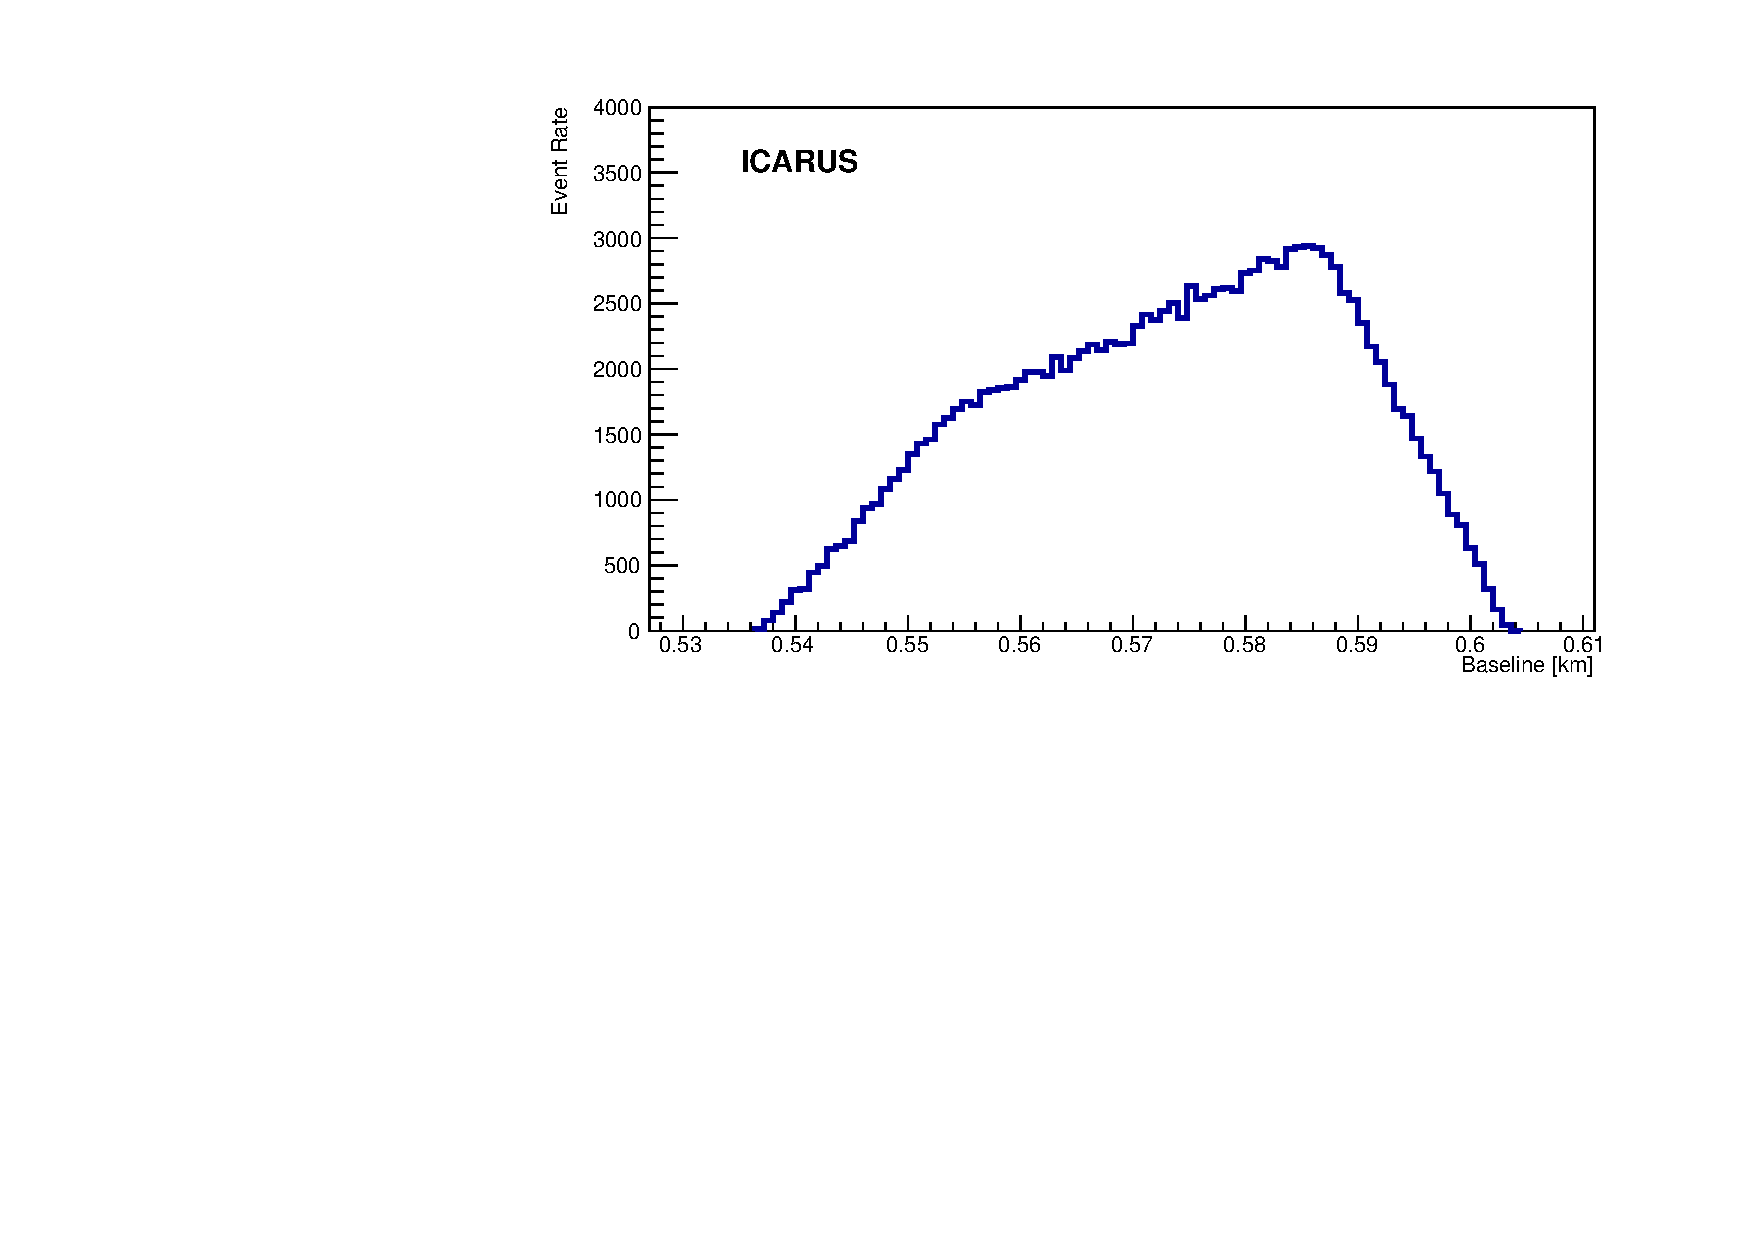
\includegraphics[width = 0.49\textwidth]{figures-chap5/ICARUS_numu.pdf}
	\captionsetup{width=0.45\textwidth}
	\parbox[b]{0.49\textwidth}%
	{
		\caption{The baseline distribution of events in the \numu sample for each of the \gls{sbn} detectors. \\\phantom{.}\\}
		\label{fig:numu_baseline}}
\end{figure}

\begin{figure}[h!]
	\centering
	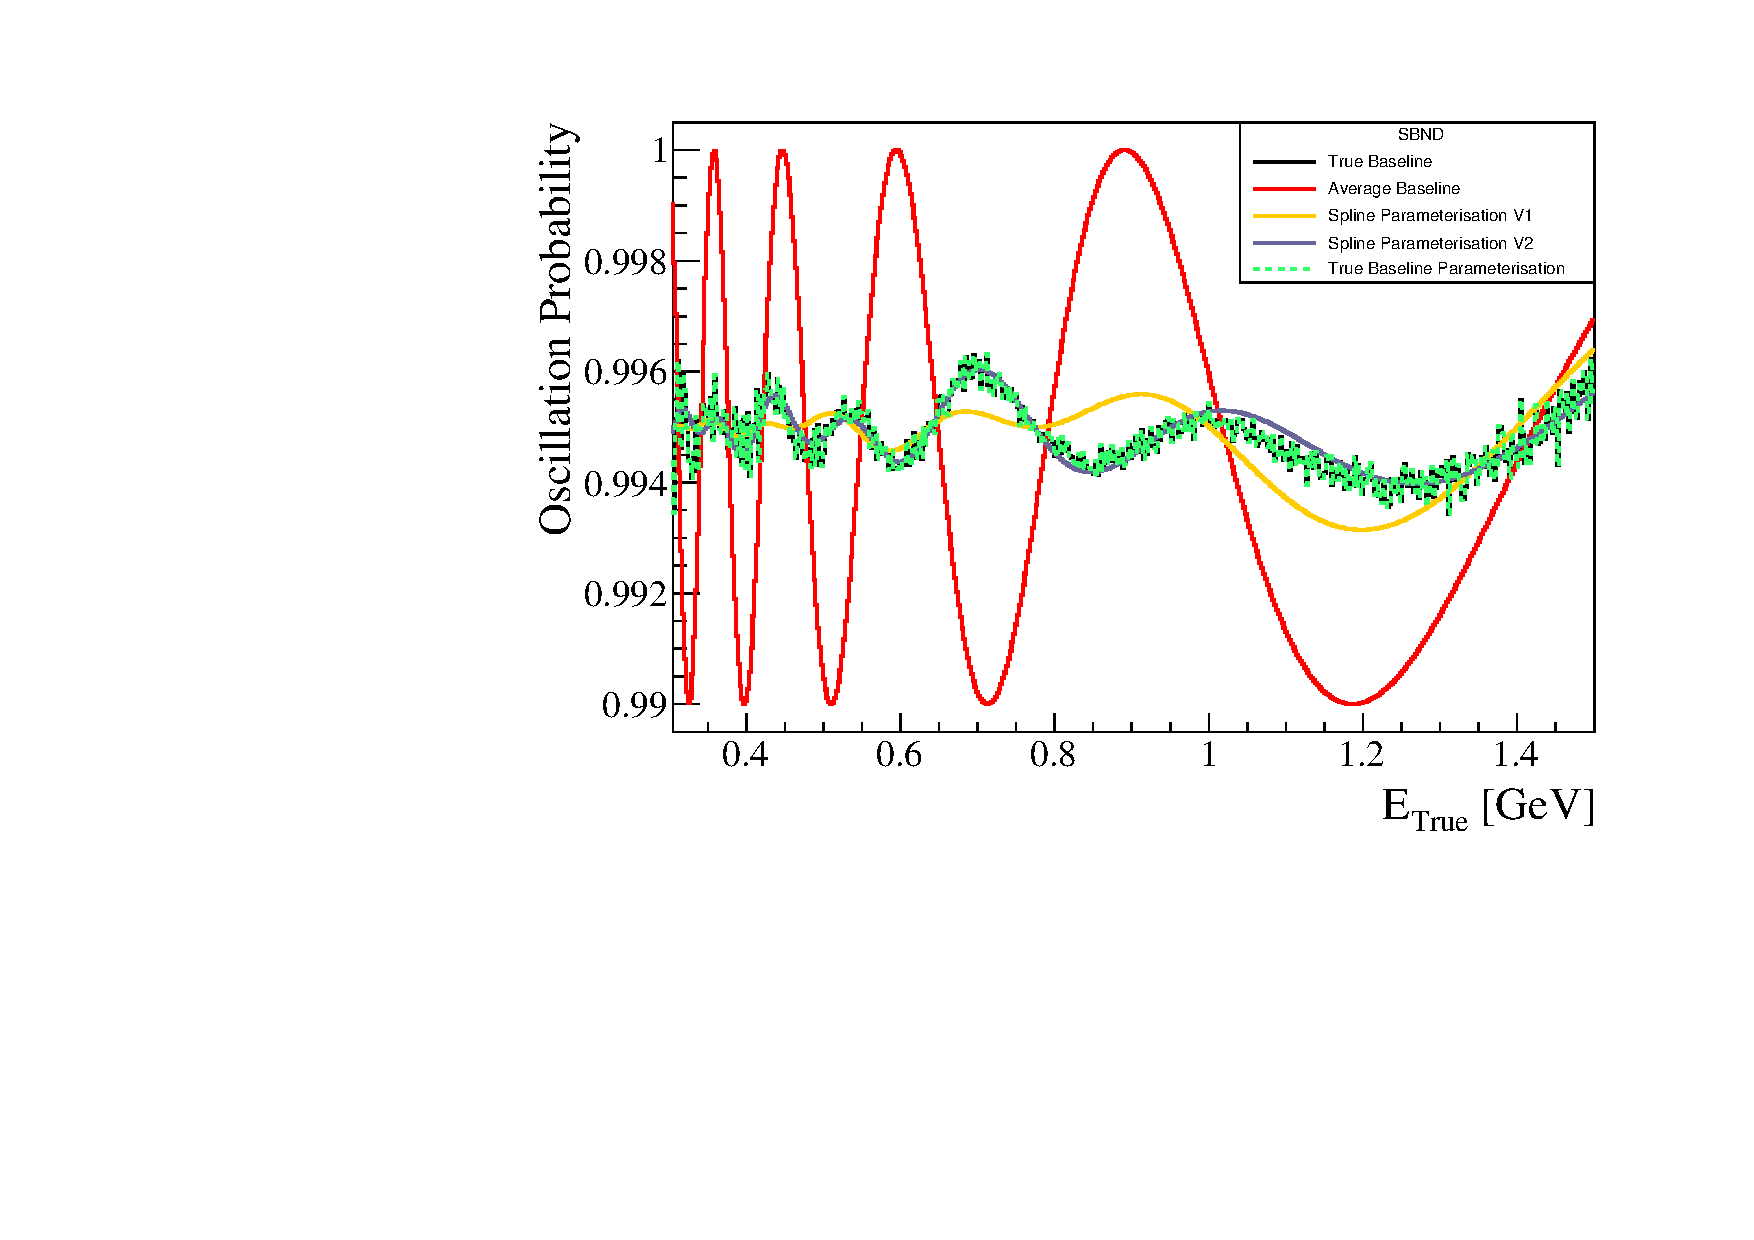
\includegraphics[width = 0.49\textwidth]{figures-chap5/osc_prob_sbnd.pdf}
	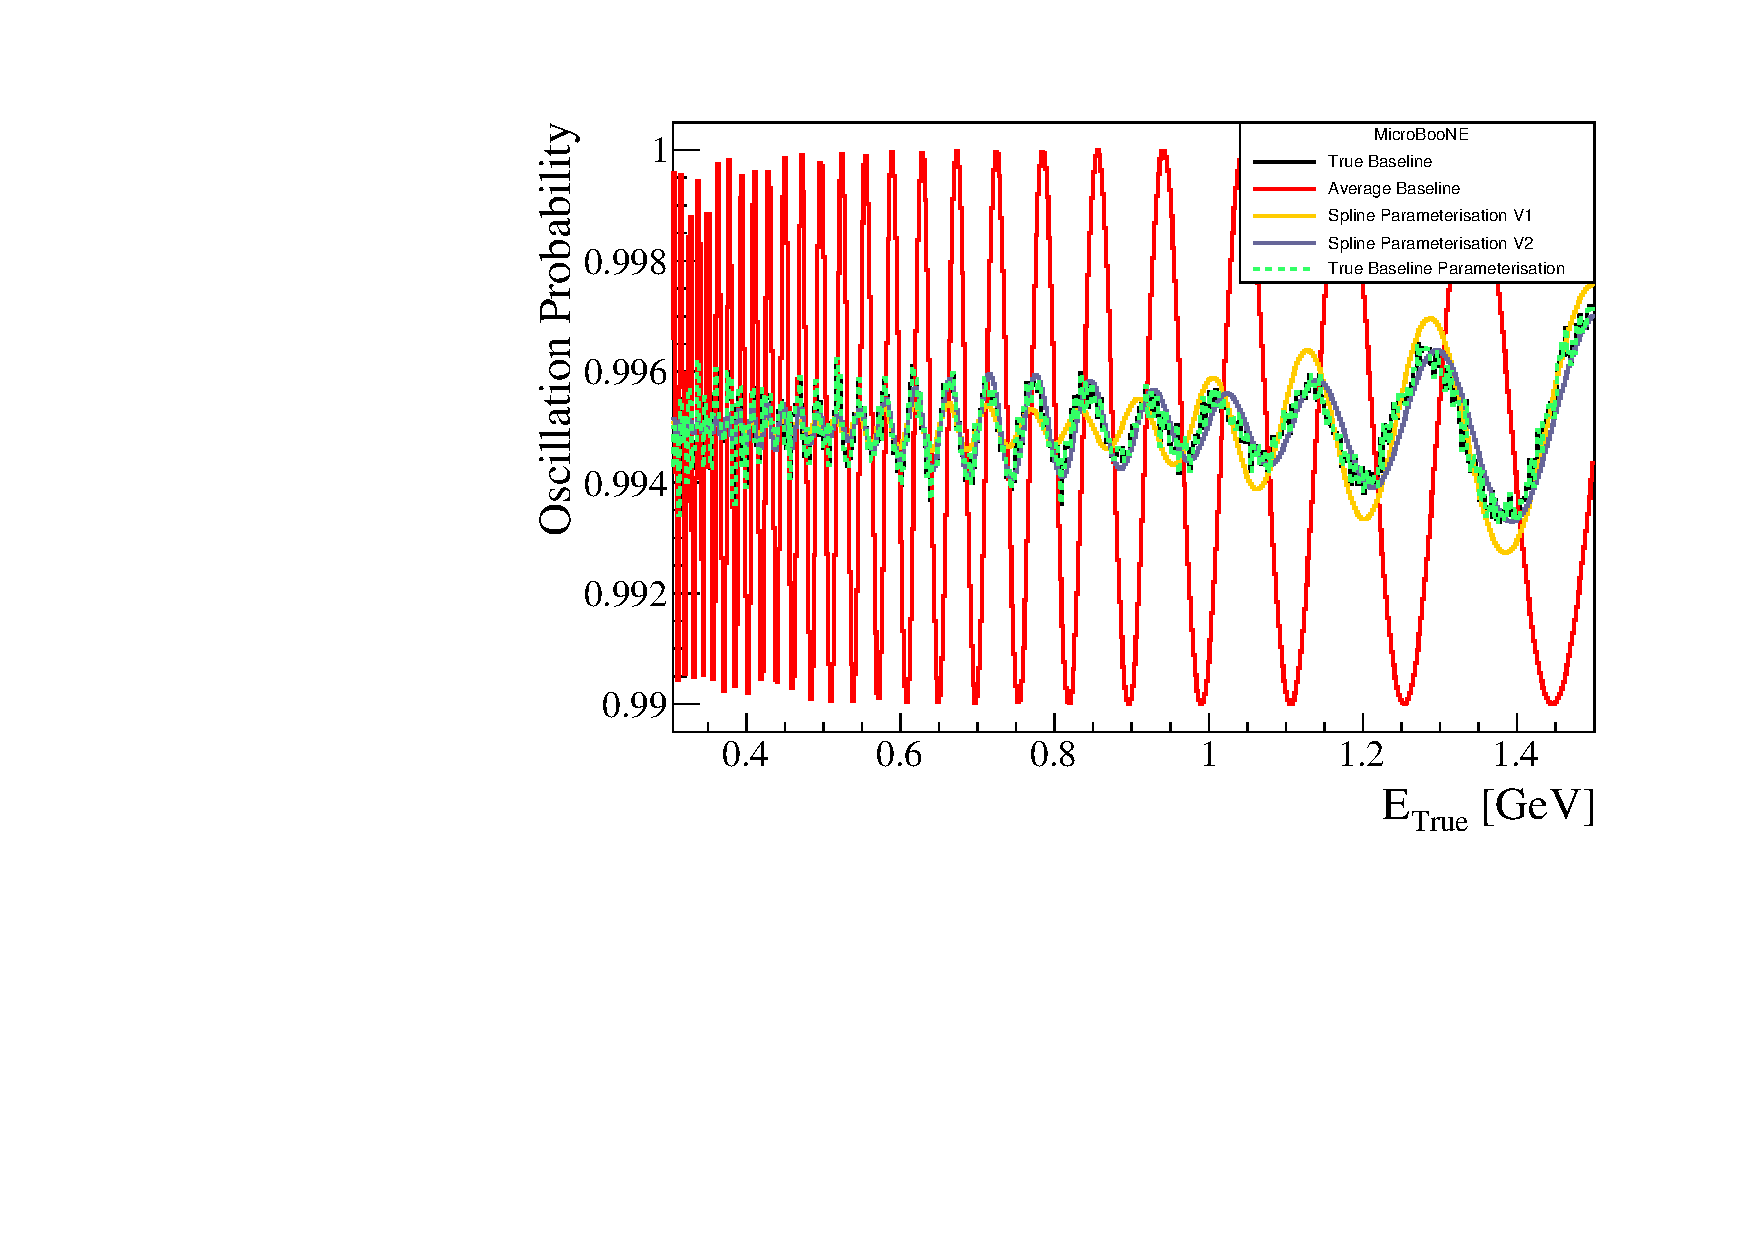
\includegraphics[width = 0.49\textwidth]{figures-chap5/osc_prob_uboone.pdf}
	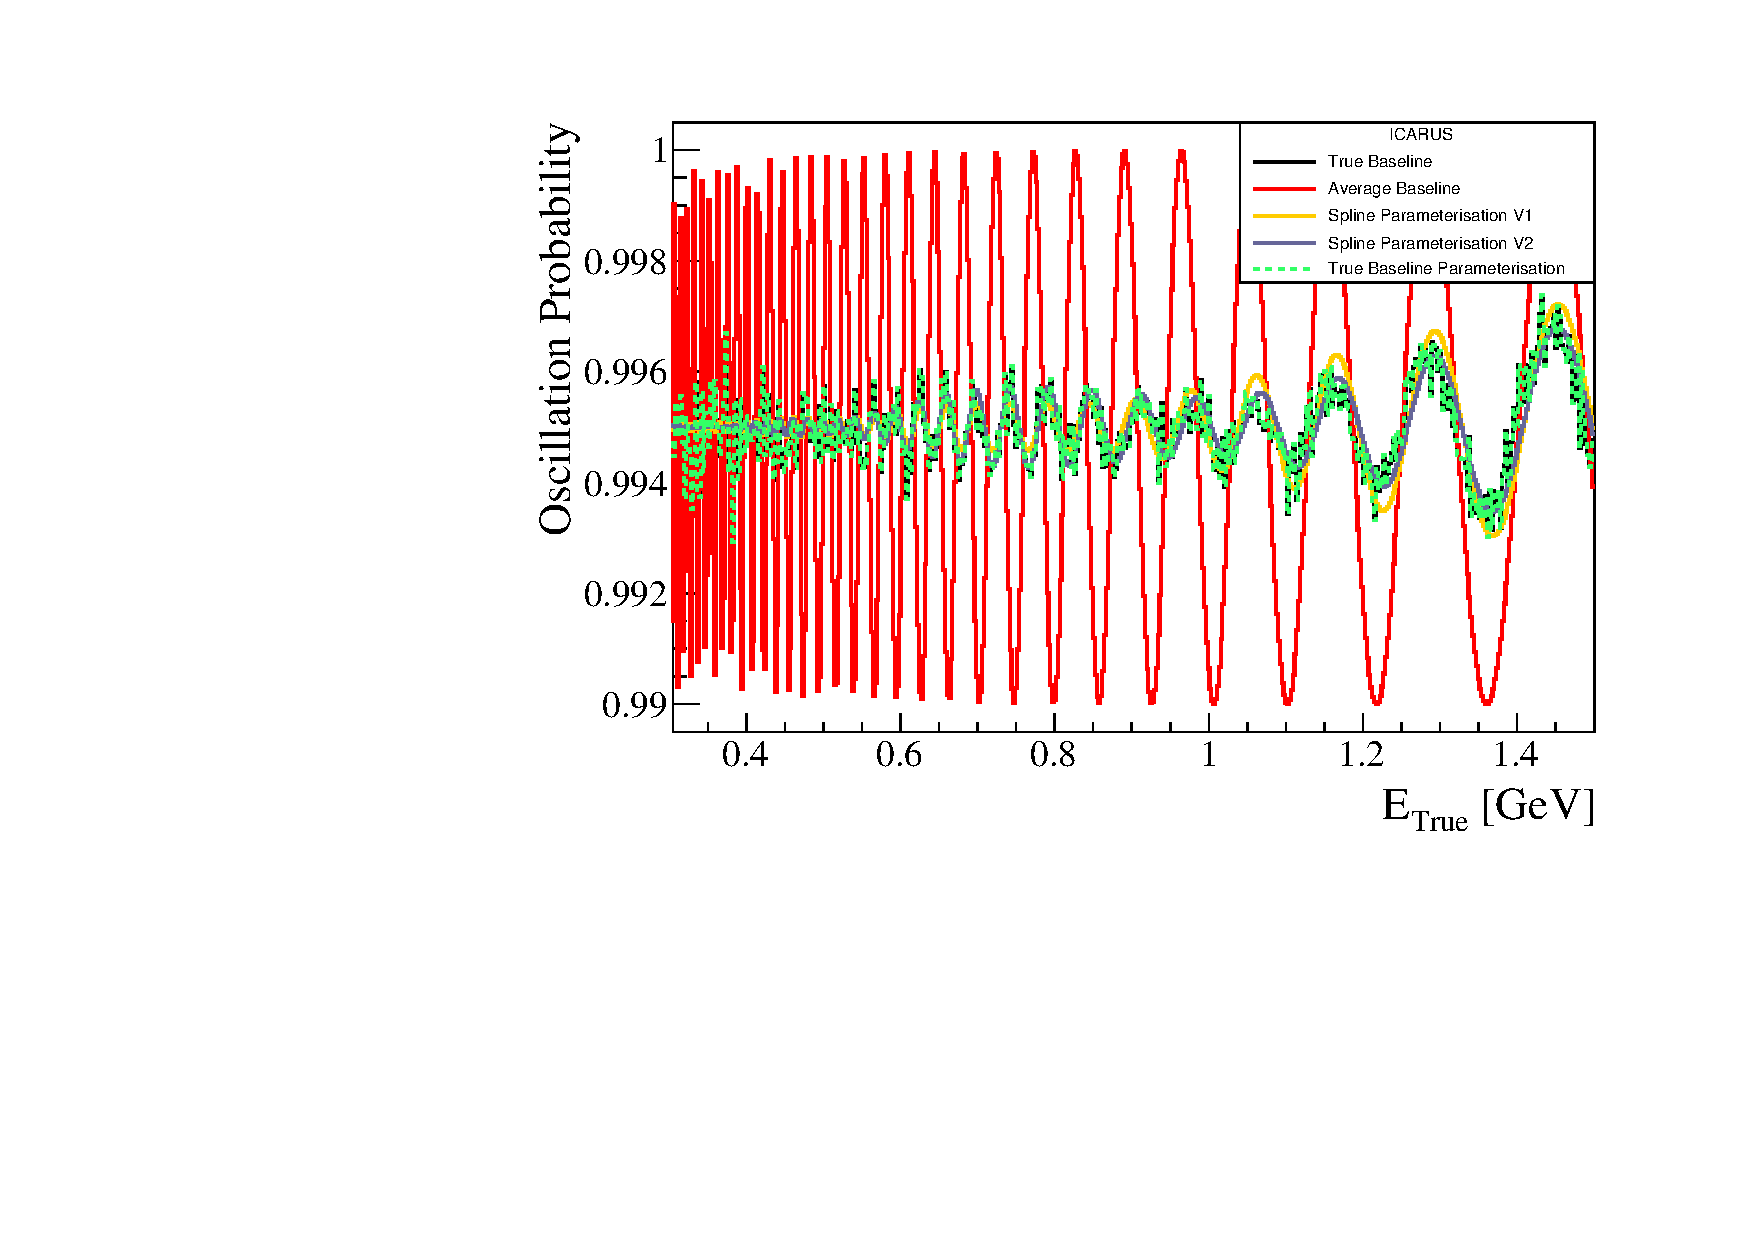
\includegraphics[width = 0.49\textwidth]{figures-chap5/osc_prob_icarus.pdf}
	\captionsetup{width=0.45\textwidth}
	\parbox[b]{0.49\textwidth}%
	{
		\caption[Oscillation probability for different baseline parametrisations.]{The oscillation probability as a function of true neutrino energy for the \numu disappearance sample with oscillation parameters $\sin^2{2\theta_{\mu\mu}} = 0.01$ and $\Delta m^2_{41} = 50$ eV$^2$ in each \gls{sbn} detector. The results from using each baseline parametrisation are shown. \\}
		\label{fig:baseline_osc_probability}}
\end{figure}
\newpage
The studies of the baseline approximations were done in the context of the \numu disappearance channel. In principle, within the \nue sample, different approximations should be applied to the different sub-samples since the baseline distribution is not the same for all the sub-samples. For example, the \numu's in the oscillated and \numu sub-samples will both mainly be the result of pion decays whereas the \nue's in the intrinsic sub-sample will have a larger contribution from kaon and secondary muon decays. Pions and kaons have different lifetimes which coupled with the contribution from the decay of secondary particles means that the baseline distribution of the oscillated and \numu sub-sample will be different to that of the intrinsic \nue sub-sample. This was never done since it was decided that the true baseline should be used. The baseline distributions for the intrinsic \nue, oscillated $\nu$ and the overall \nue sample from combining all the sub-samples together are shown in \FigureRef{fig:nue_intrinsic_baseline}, \FigureRef{fig:nue_osc_baseline} and \FigureRef{fig:nue_baseline} respectively for each of the \gls{sbn} detectors. It should be noted that the baseline distributions for oscillated \nue sample from \FigureRef{fig:nue_osc_baseline} and the \numu sample from \FigureRef{fig:numu_baseline} are comparable. This is due to the initial parameters describing the oscillated sample being the same as for the \numu sample. The only difference being the neutrino oscillations from \numu to \nue which is not something that affects the baseline.

\begin{comment}
\begin{figure}[!h]
    \centering
    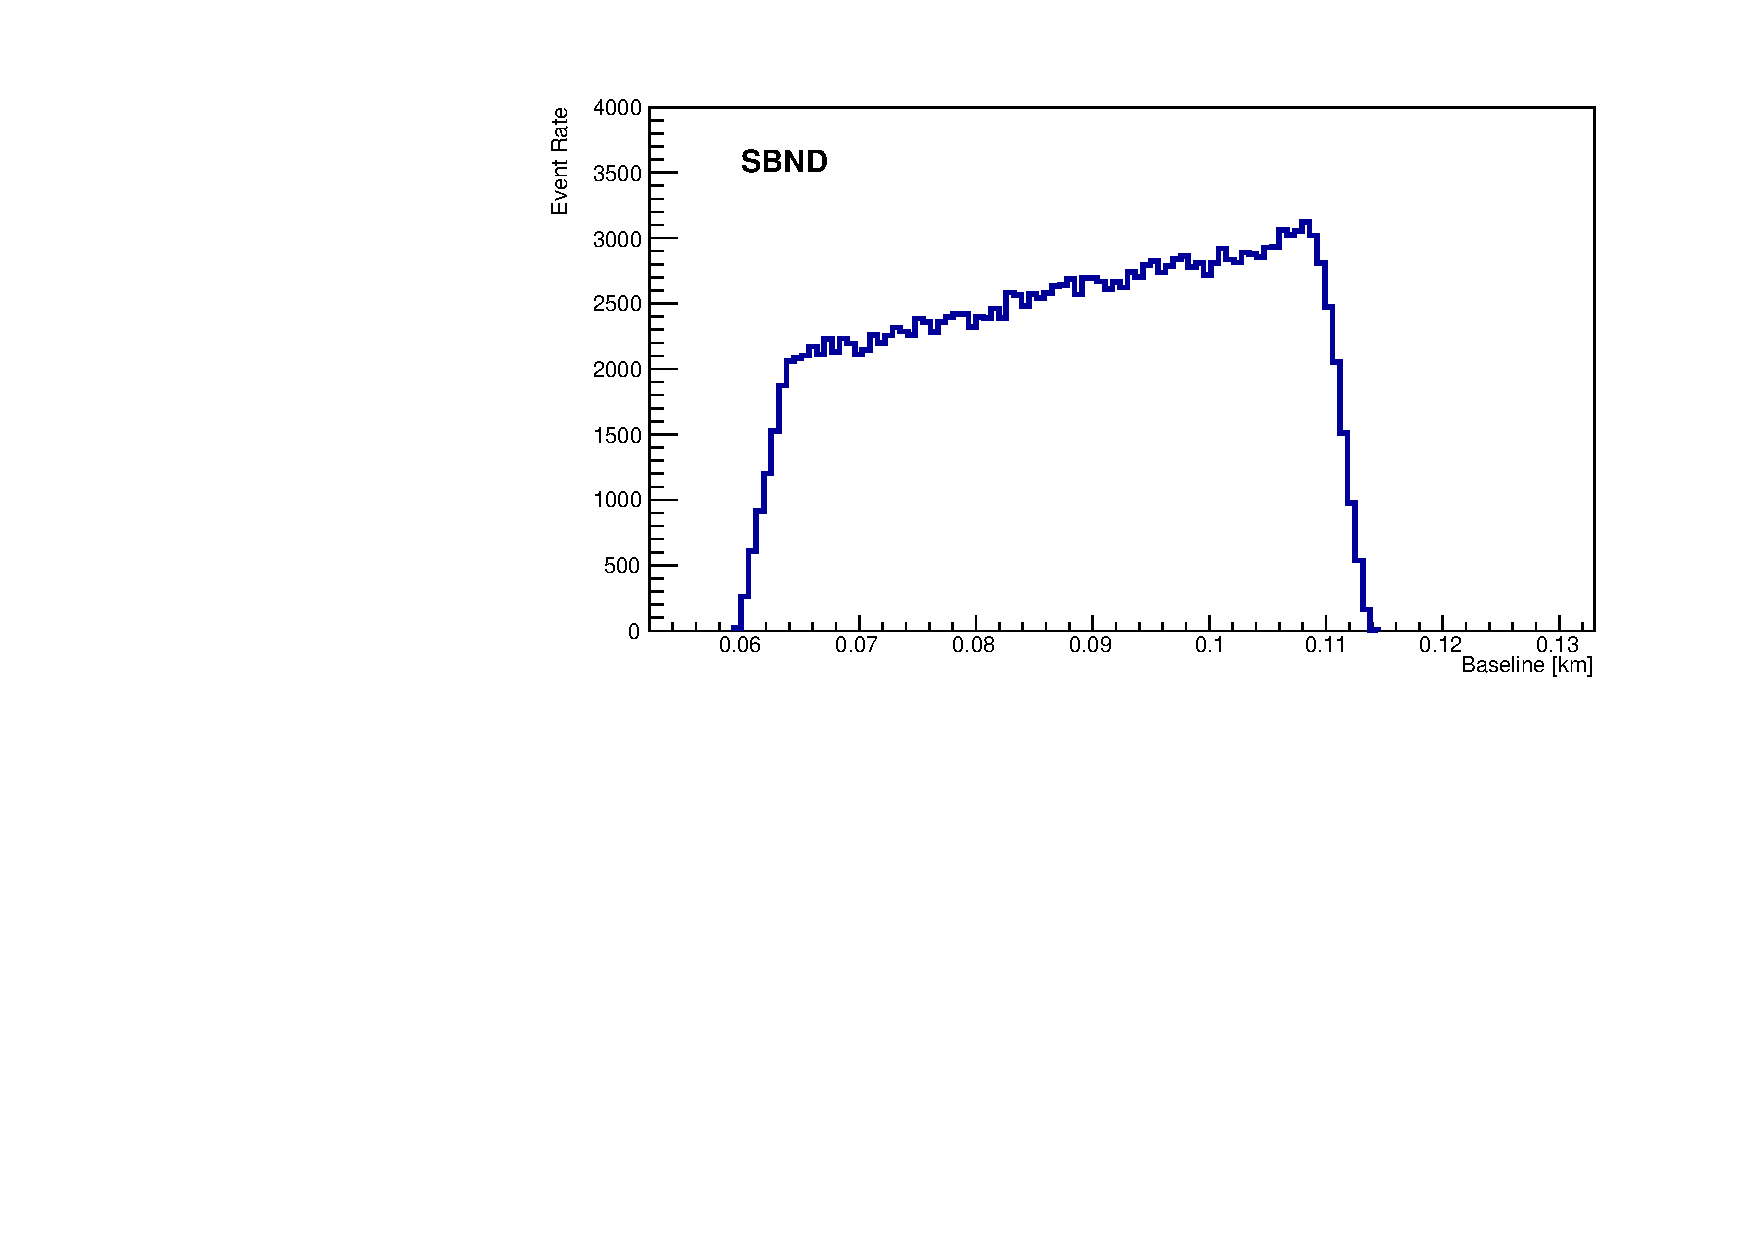
\includegraphics[width = 0.32\textwidth]{figures-chap5/SBND_numu.pdf}
    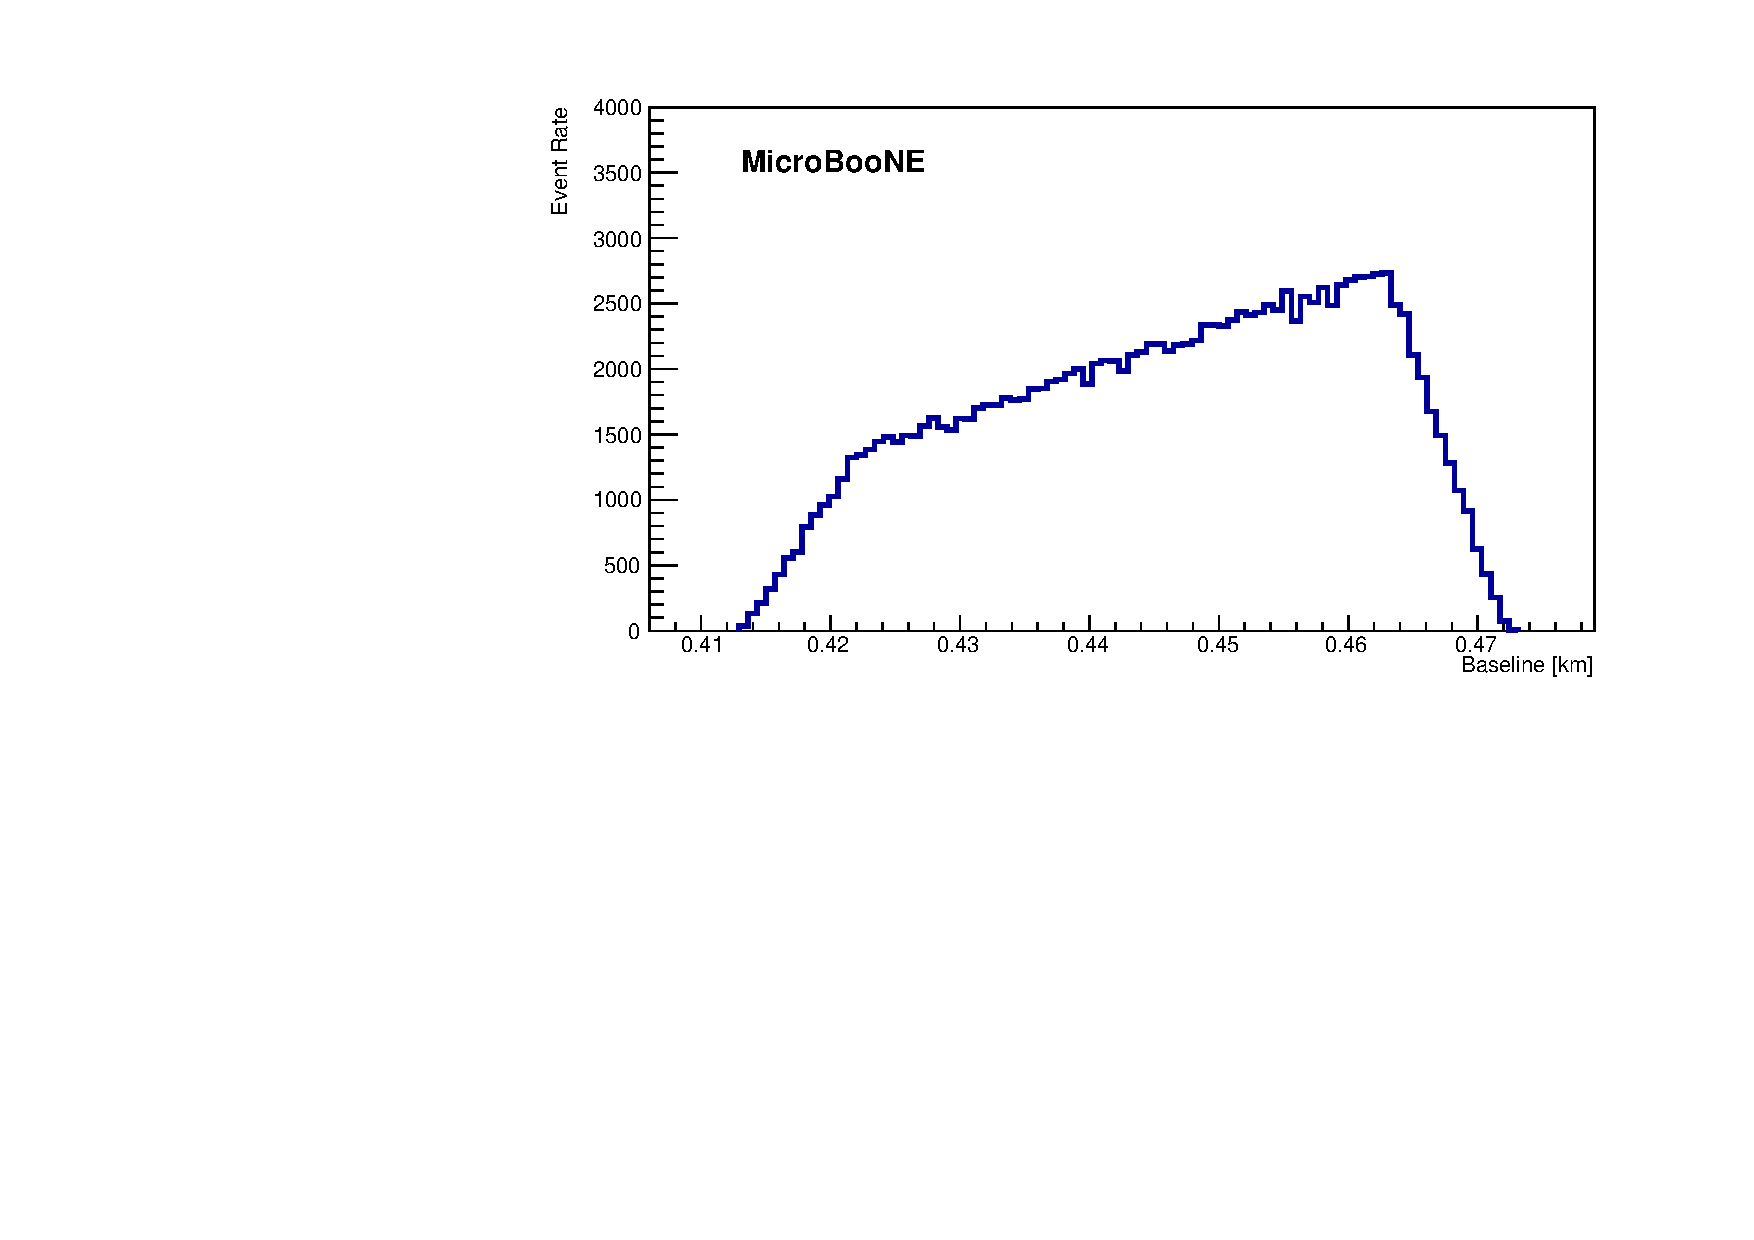
\includegraphics[width = 0.32\textwidth]{figures-chap5/MicroBooNE_numu.pdf}
    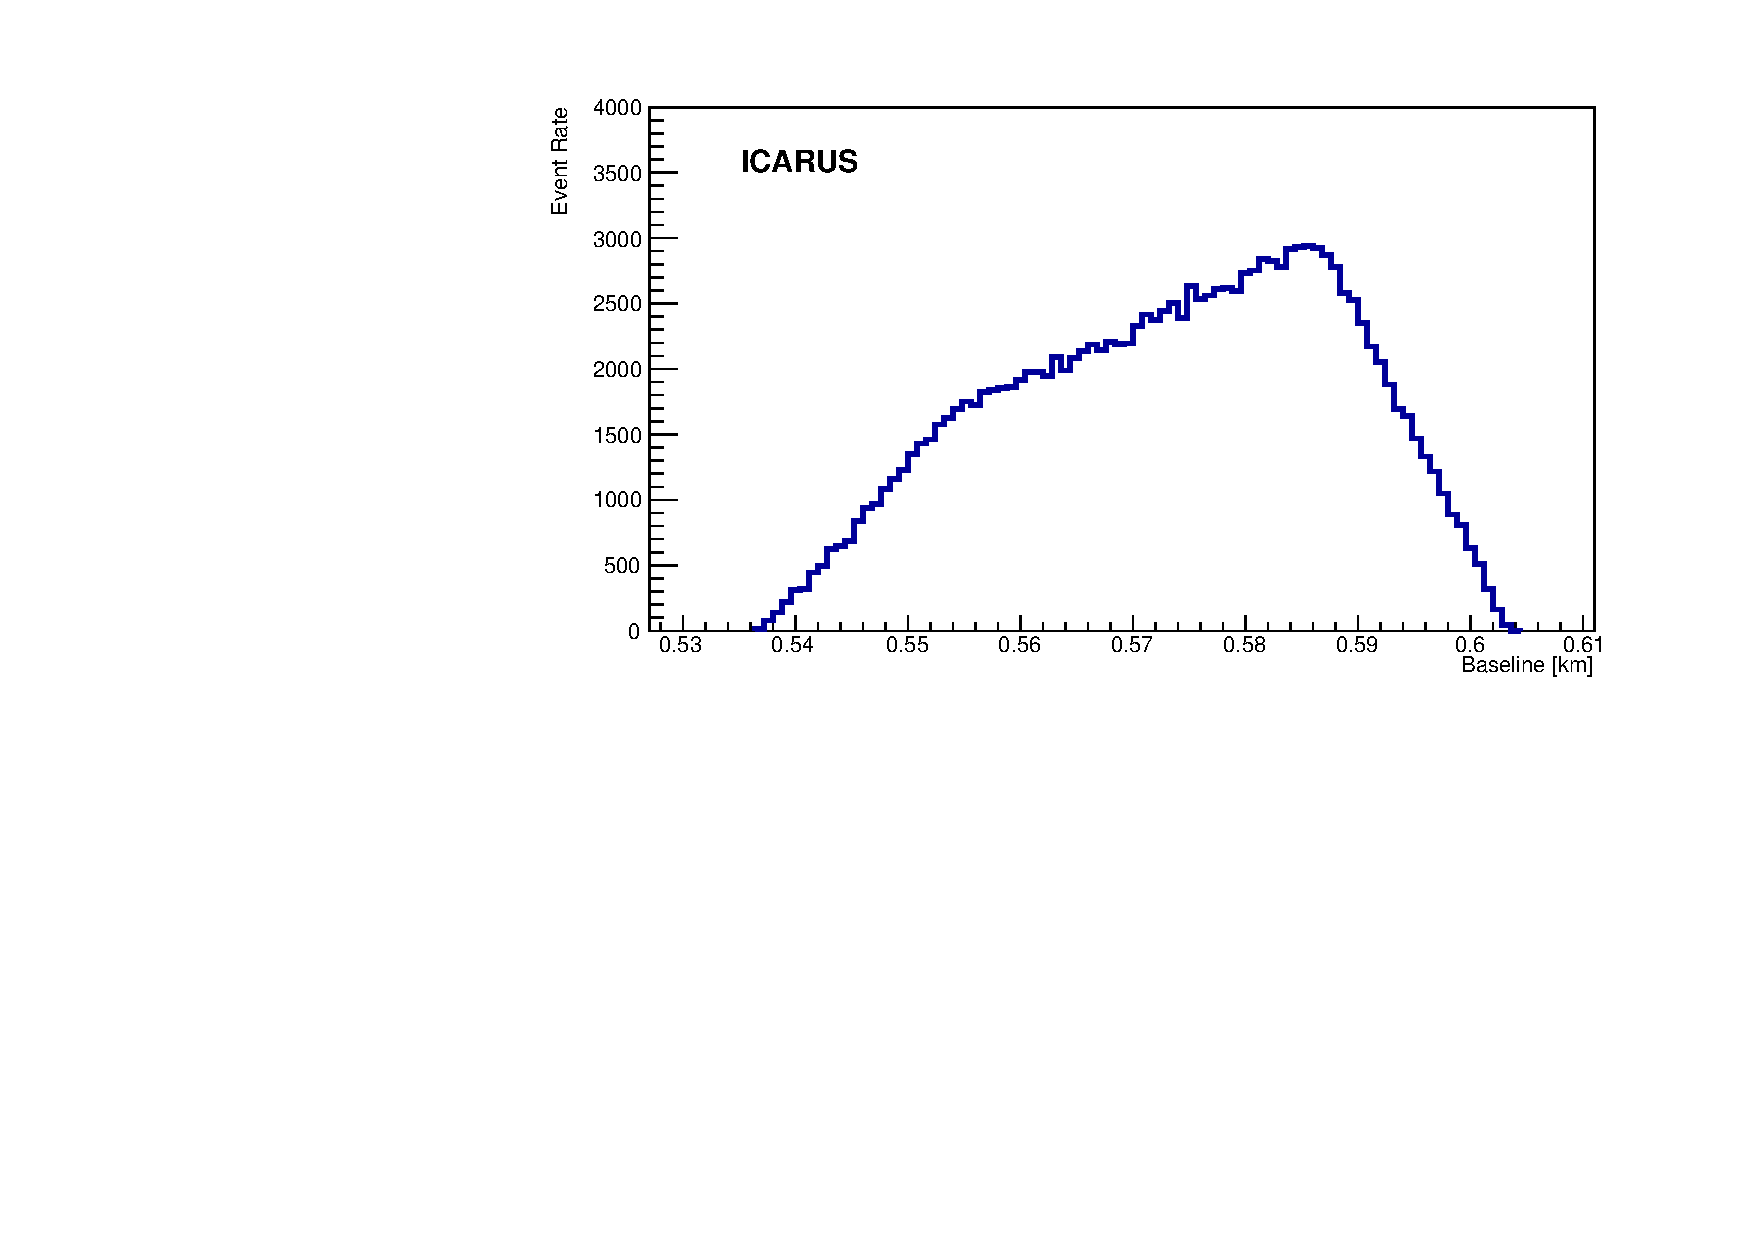
\includegraphics[width = 0.32\textwidth]{figures-chap5/ICARUS_numu.pdf}
    \caption{The baseline distribution of events in the \numu sample for each of the \gls{sbn} detectors.}
    \label{fig:numu_baseline}
\end{figure}
\end{comment}


\begin{figure}[h!]
    \centering
    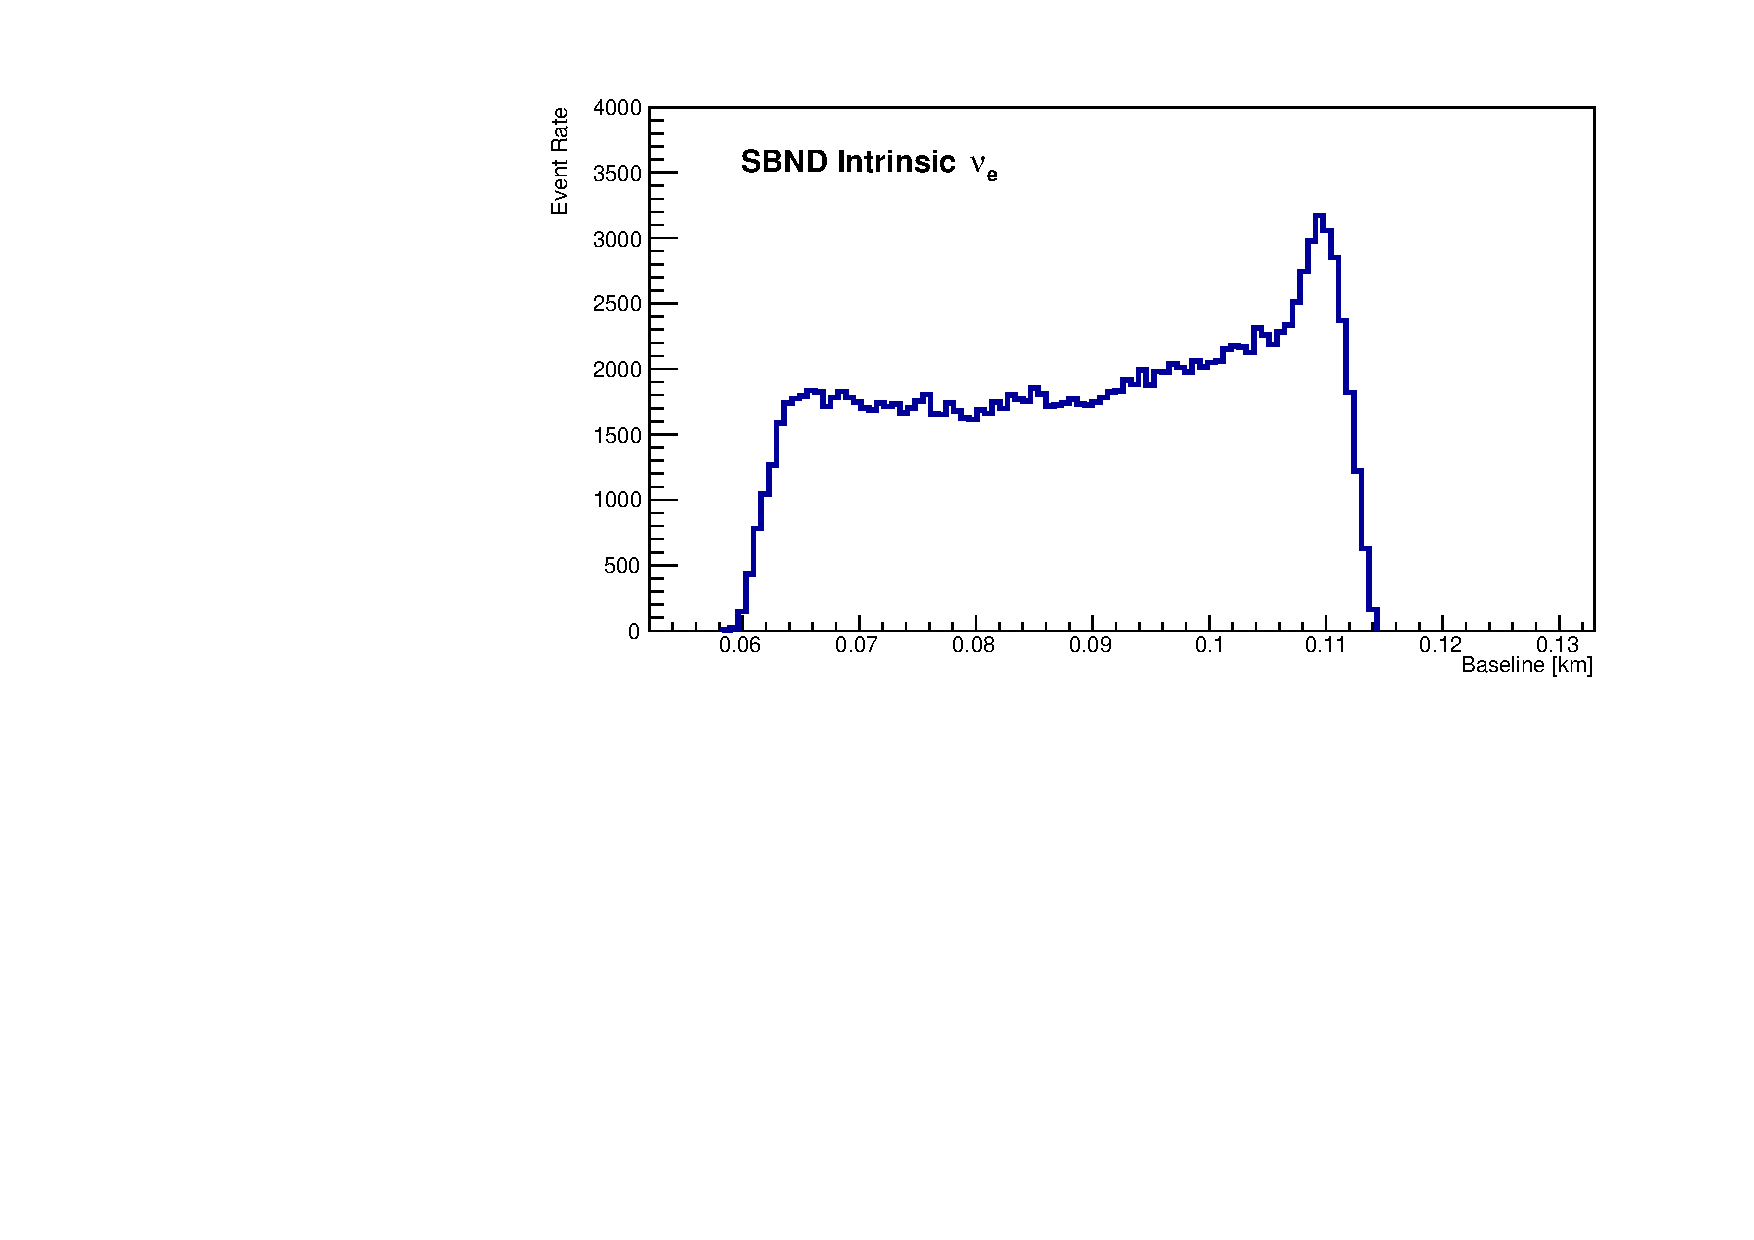
\includegraphics[width = 0.49\textwidth]{figures-chap5/SBND_intrinsic_nue.pdf}
    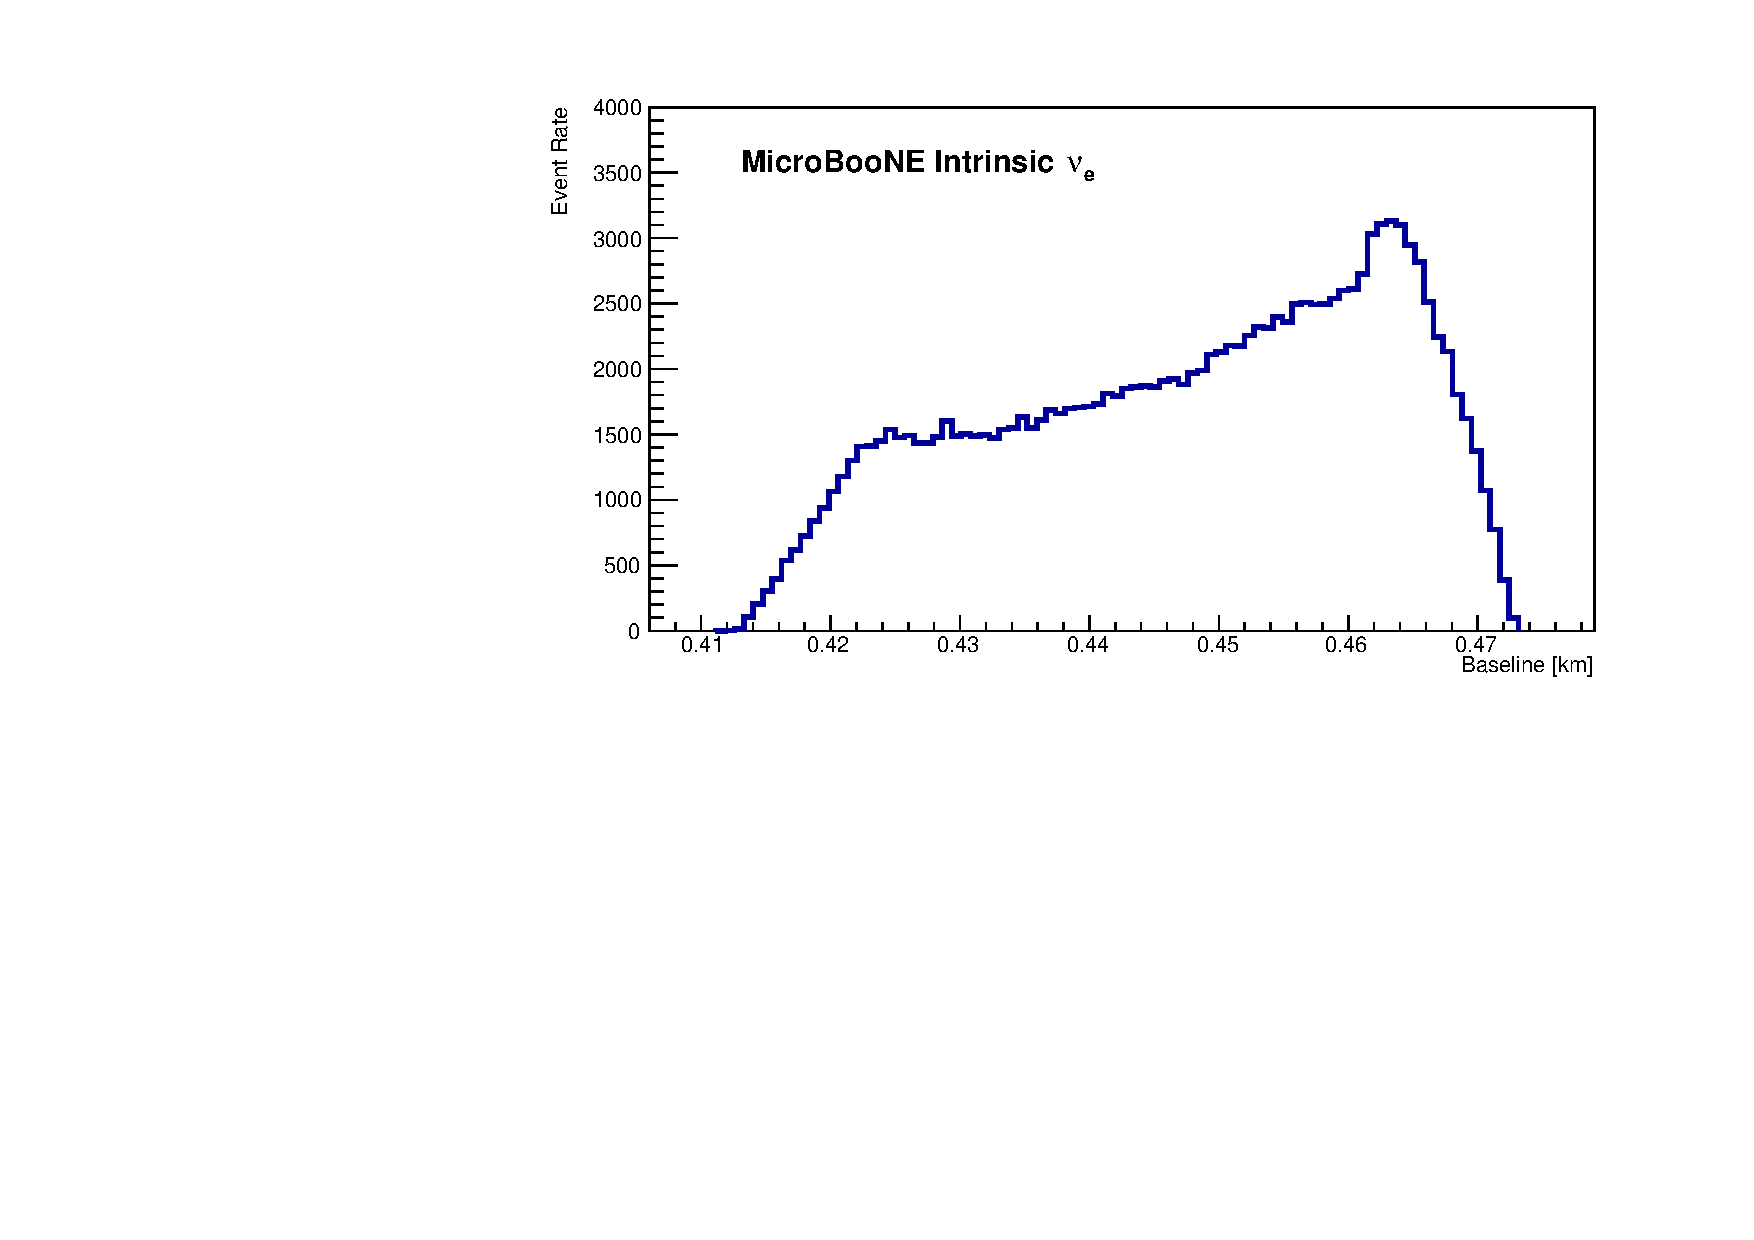
\includegraphics[width = 0.49\textwidth]{figures-chap5/MicroBooNE_intrinsic_nue.pdf}
    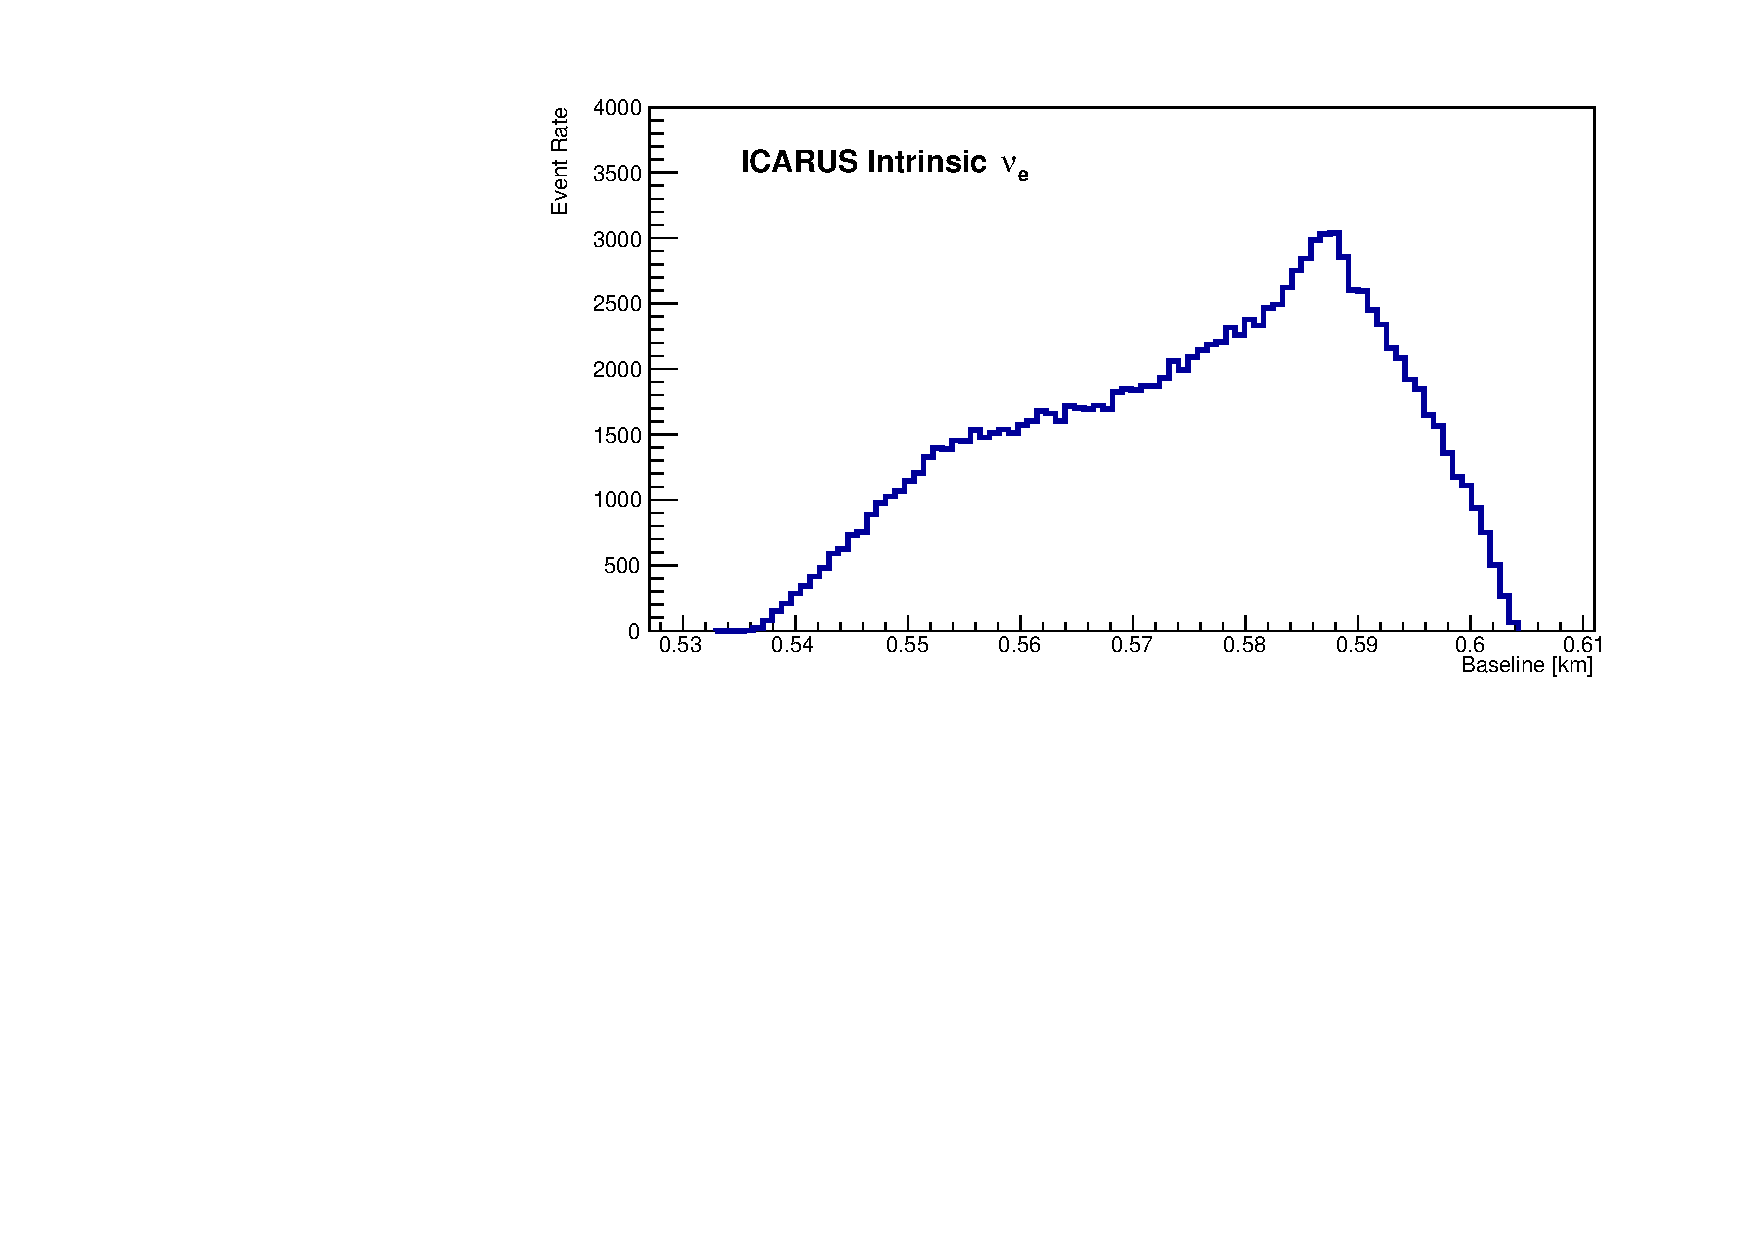
\includegraphics[width = 0.49\textwidth]{figures-chap5/ICARUS_intrinsic_nue.pdf} 
    \captionsetup{width=0.45\textwidth}
    \parbox[b]{0.49\textwidth}%
    {
    \caption{The baseline distribution of events in the intrinsic \nue sample for each of the \gls{sbn} detectors. \\\phantom{.}\\}
    \label{fig:nue_intrinsic_baseline}
    }
  \end{figure}
  
  \begin{figure}[h!]
    \centering
    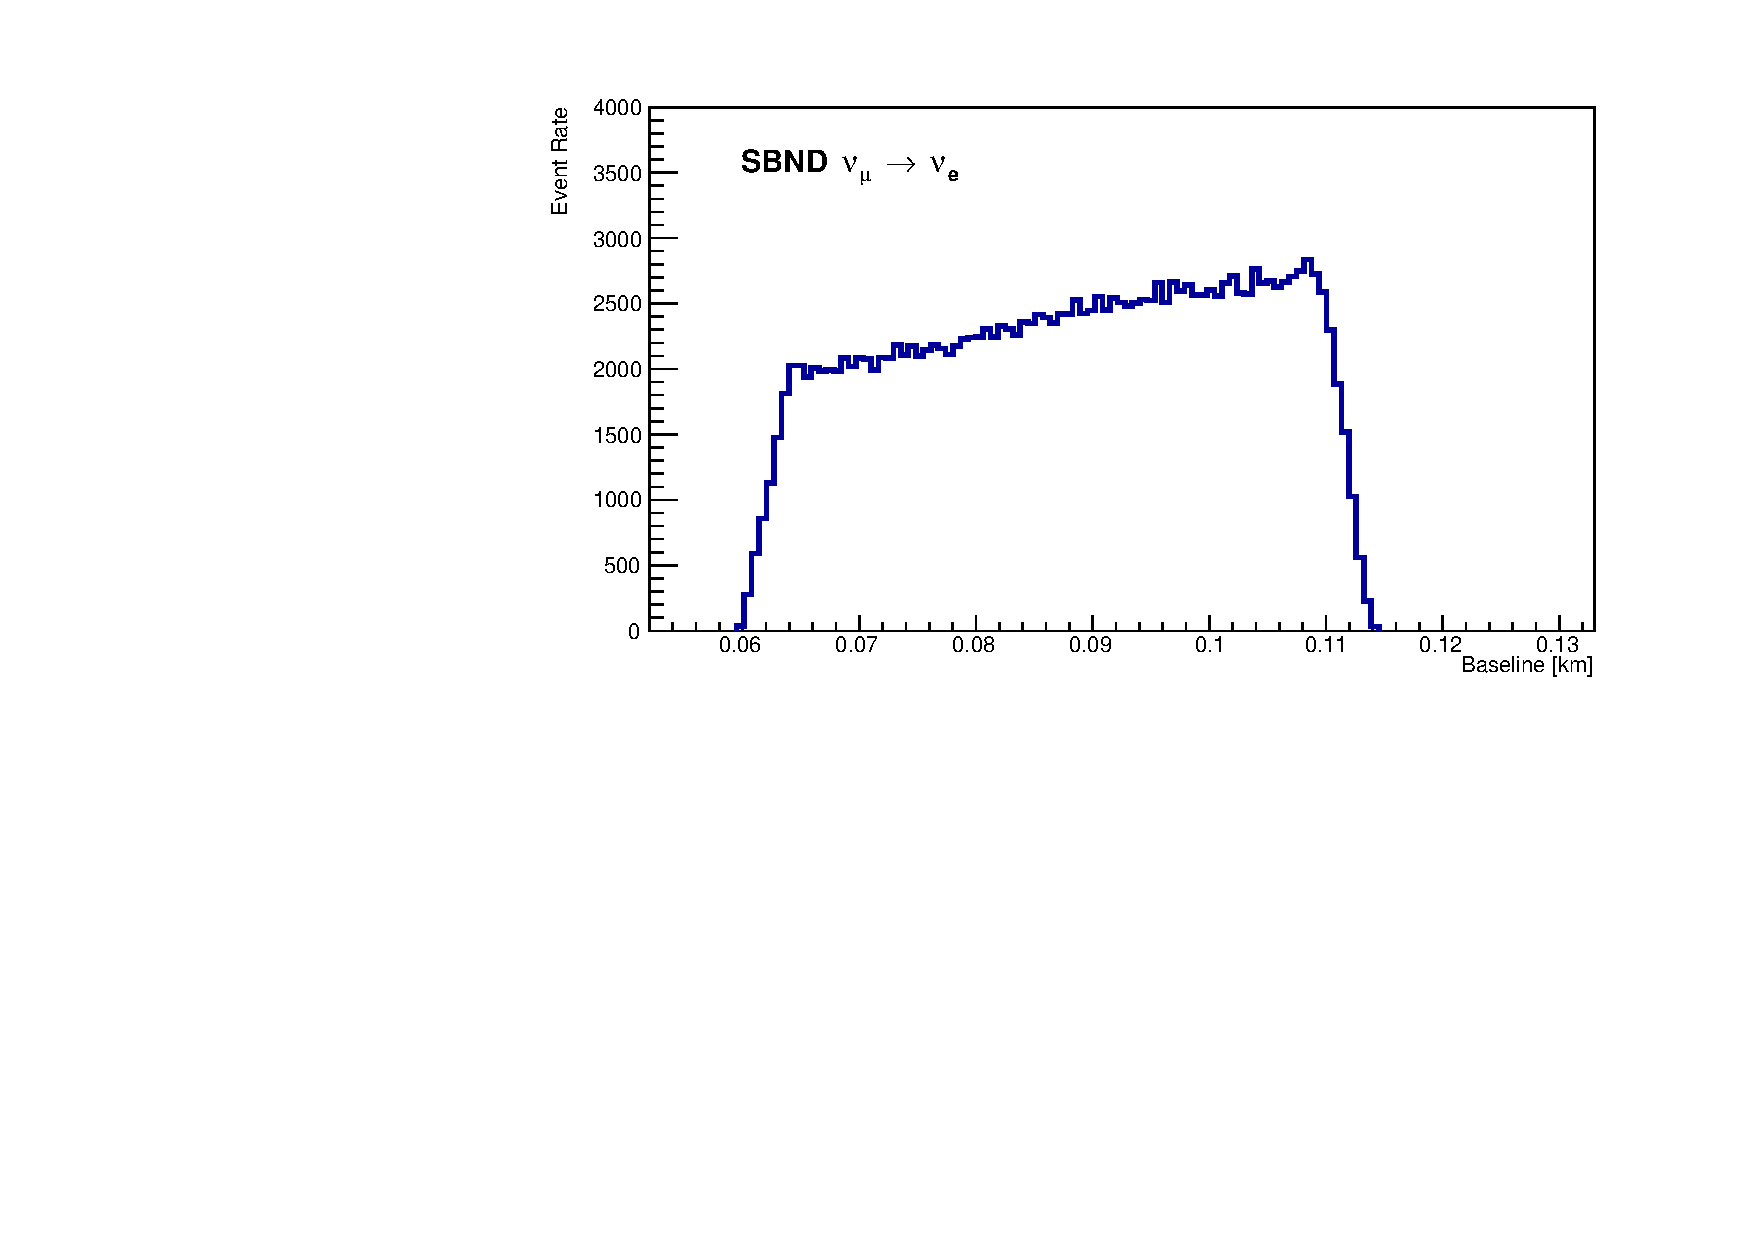
\includegraphics[width = 0.49\textwidth]{figures-chap5/SBND_osc.pdf}
    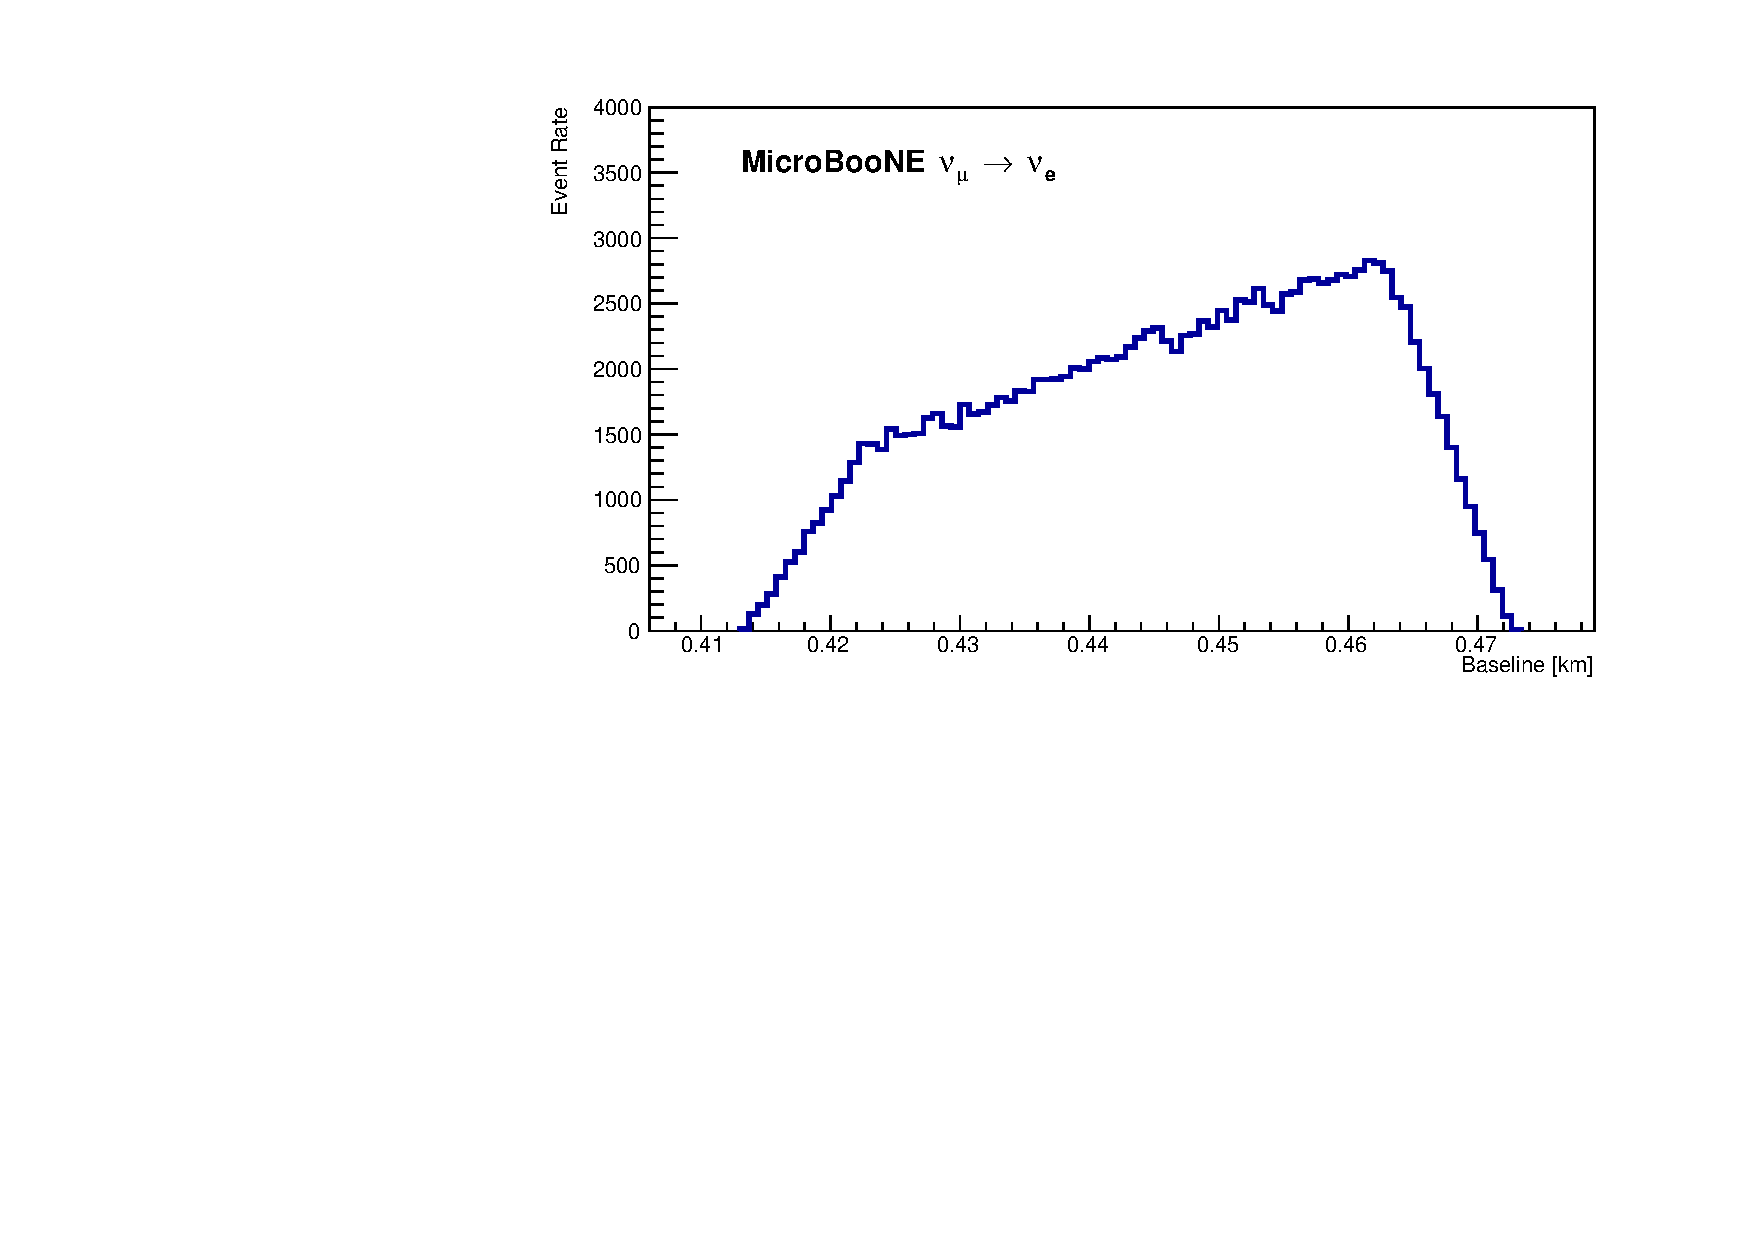
\includegraphics[width = 0.49\textwidth]{figures-chap5/MicroBooNE_osc.pdf}
    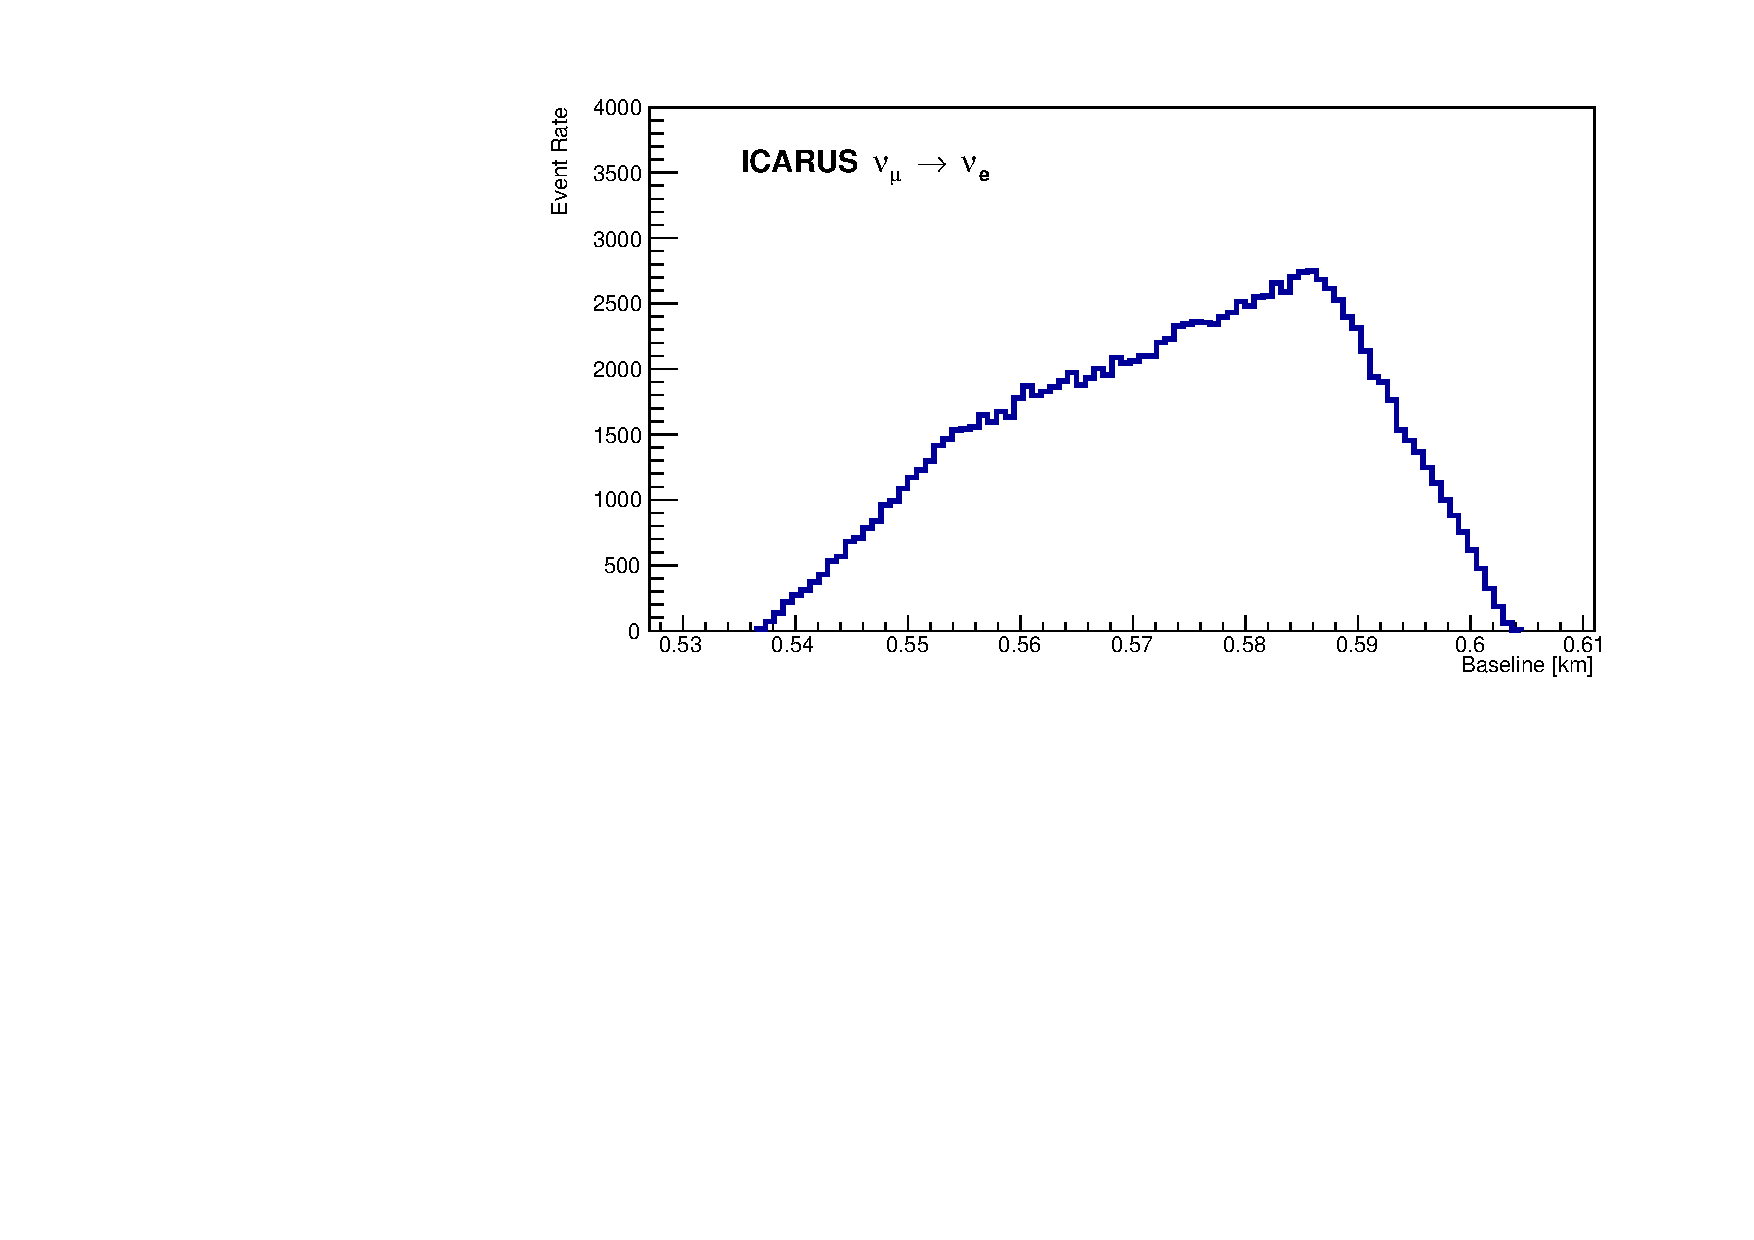
\includegraphics[width = 0.49\textwidth]{figures-chap5/ICARUS_osc.pdf}
    \captionsetup{width=0.45\textwidth}
    \parbox[b]{0.49\textwidth}%
    {
    \caption{The baseline distribution of events in the oscillated $\numu \rightarrow \nue$ sample for each of the \gls{sbn} detectors. \\\phantom{.}\\}
    \label{fig:nue_osc_baseline}
    }
  \end{figure}
  
  \begin{figure}[h!]
    \centering
    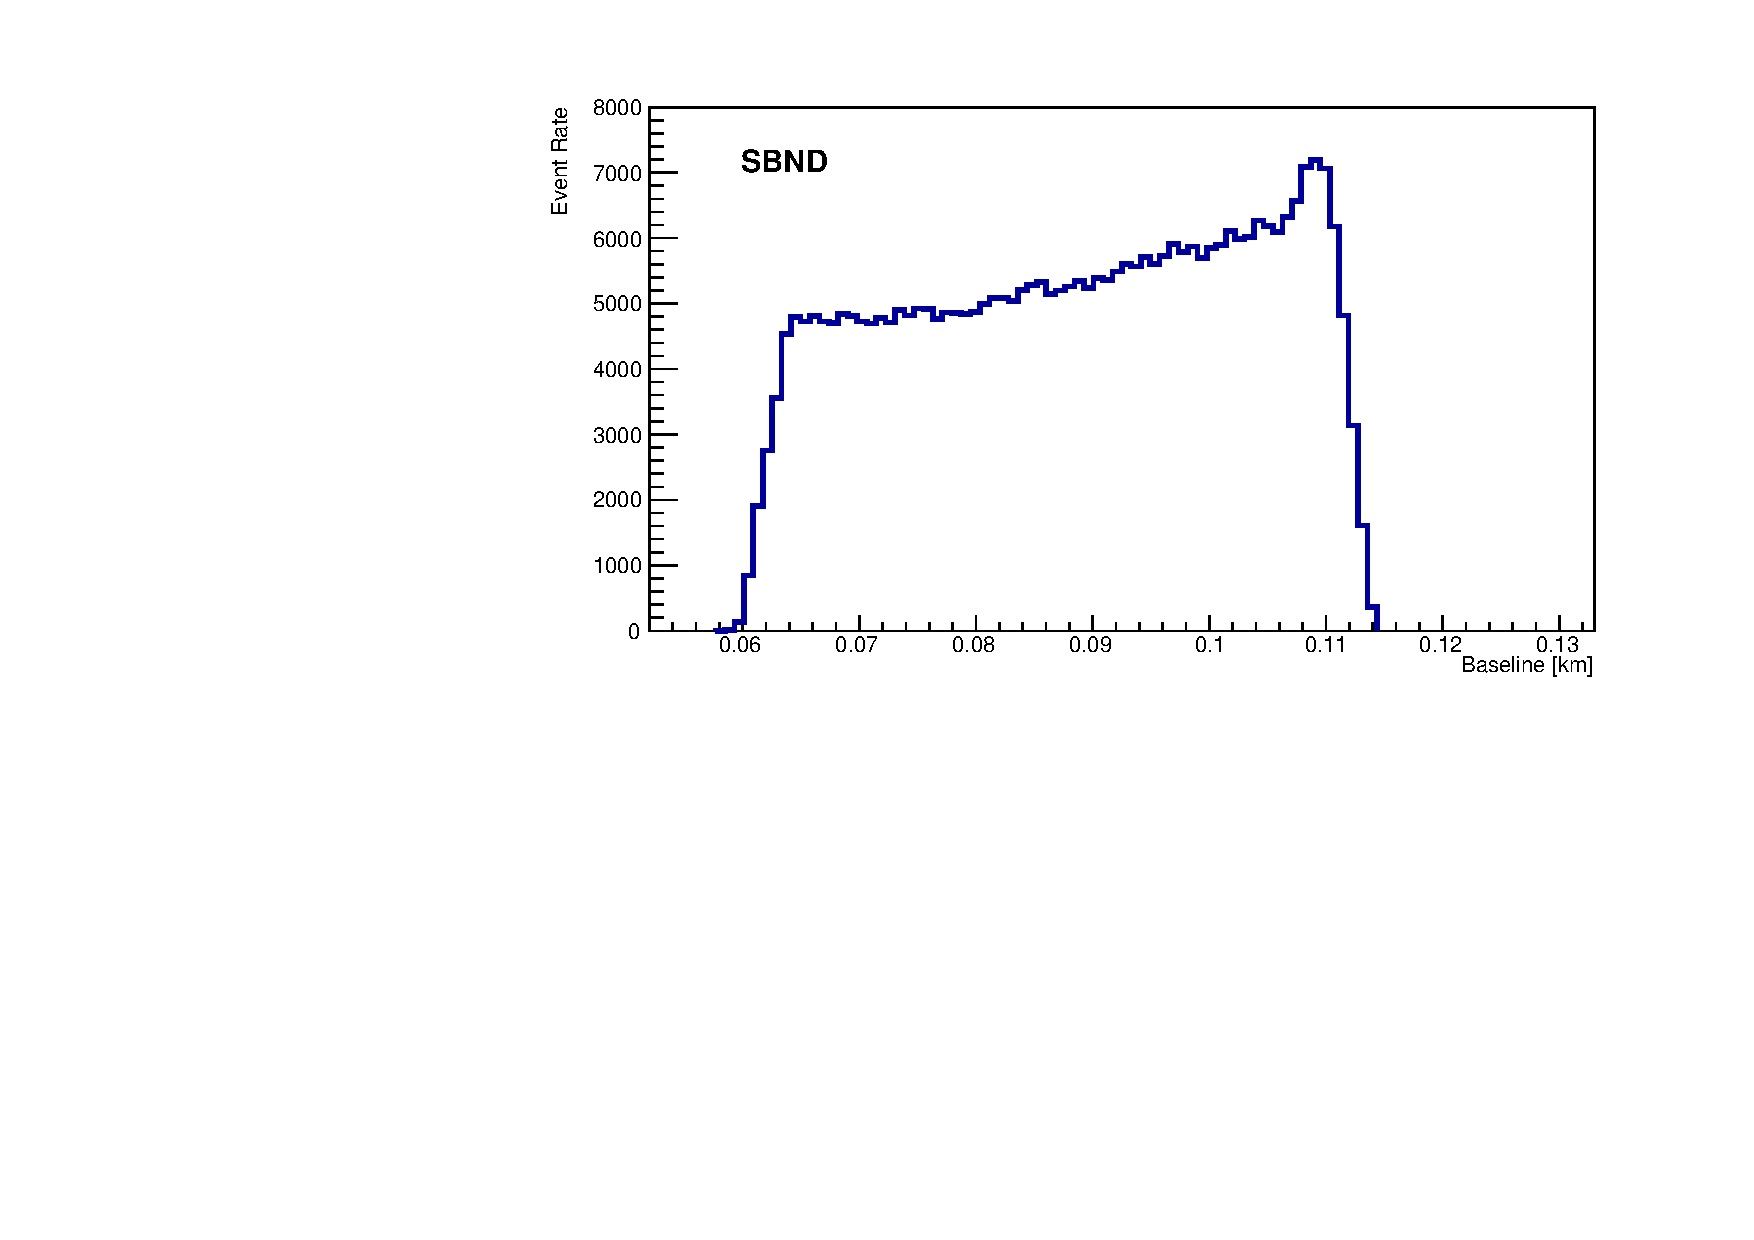
\includegraphics[width = 0.49\textwidth]{figures-chap5/SBND_nue.pdf}
    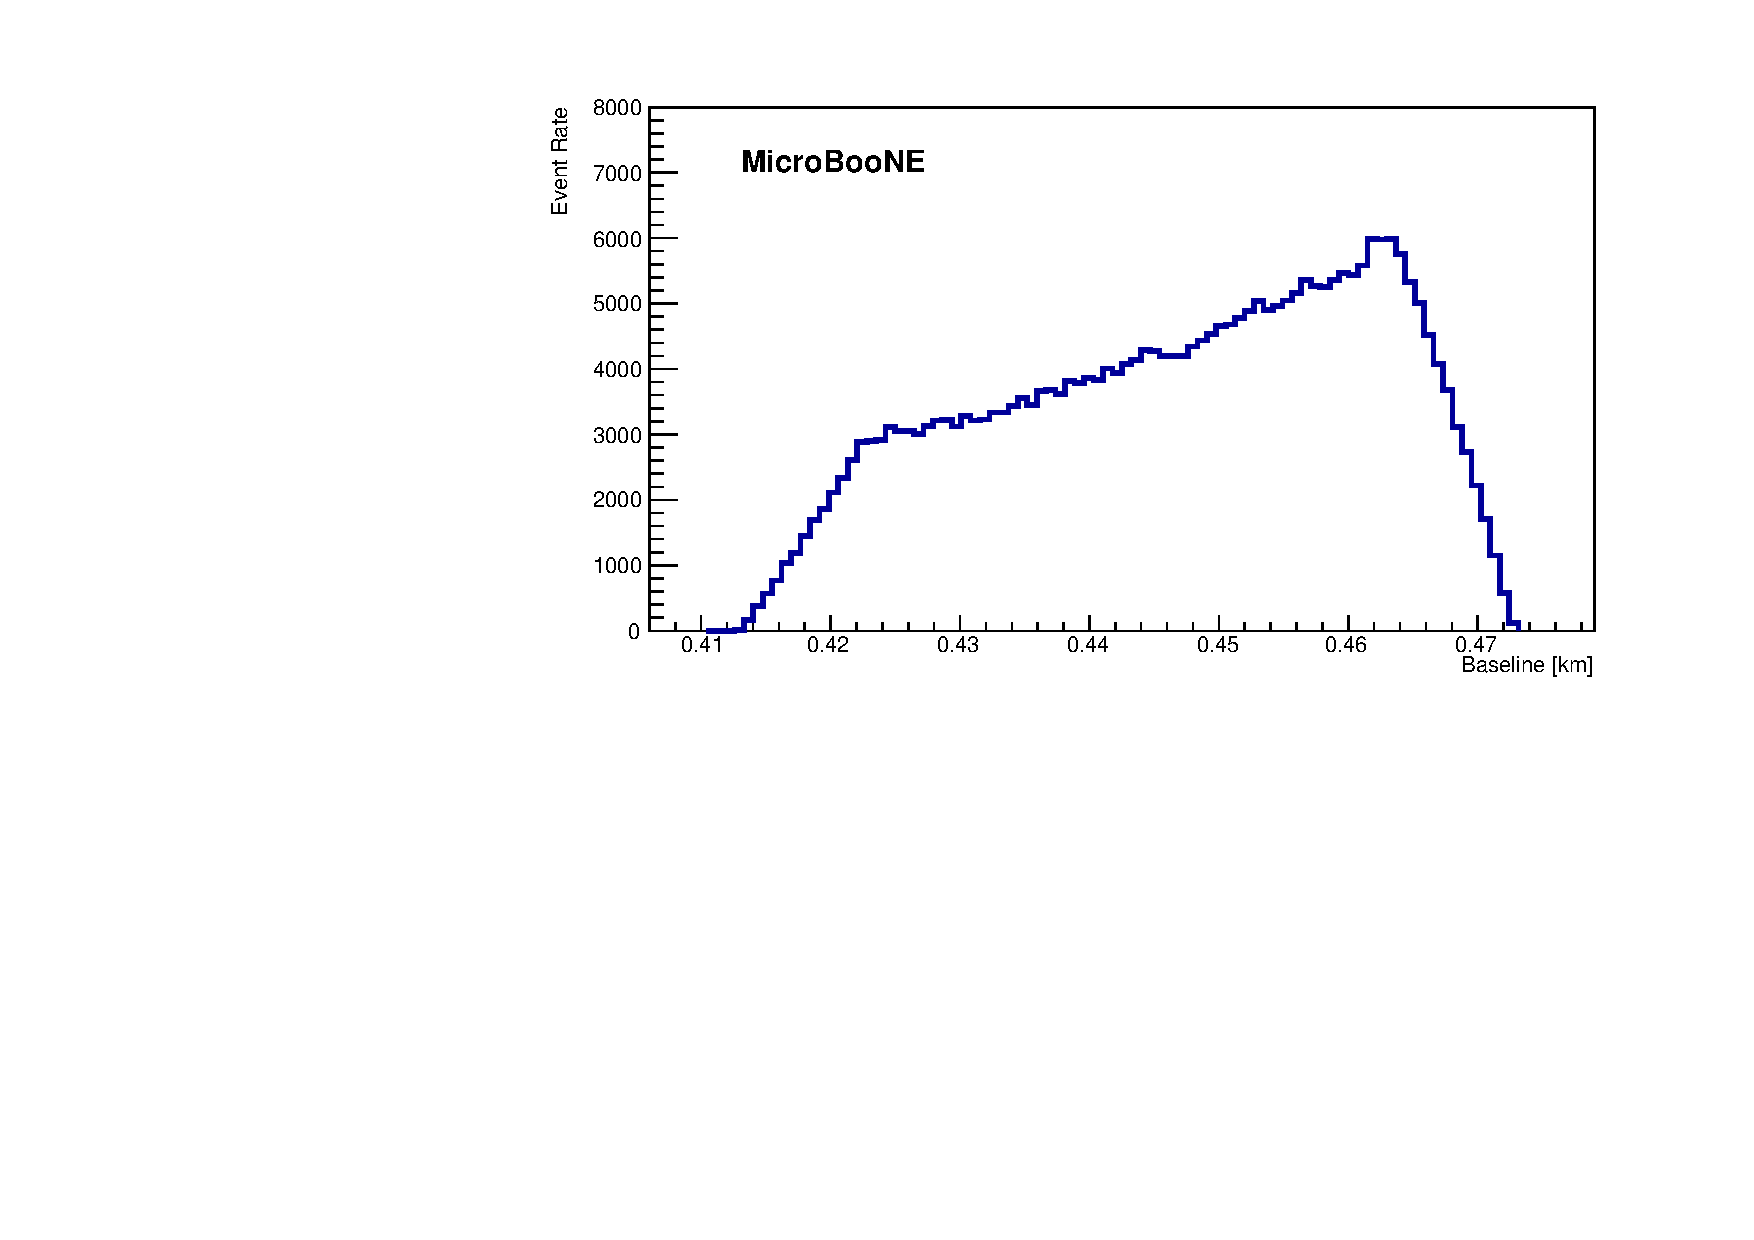
\includegraphics[width = 0.49\textwidth]{figures-chap5/MicroBooNE_nue.pdf}
    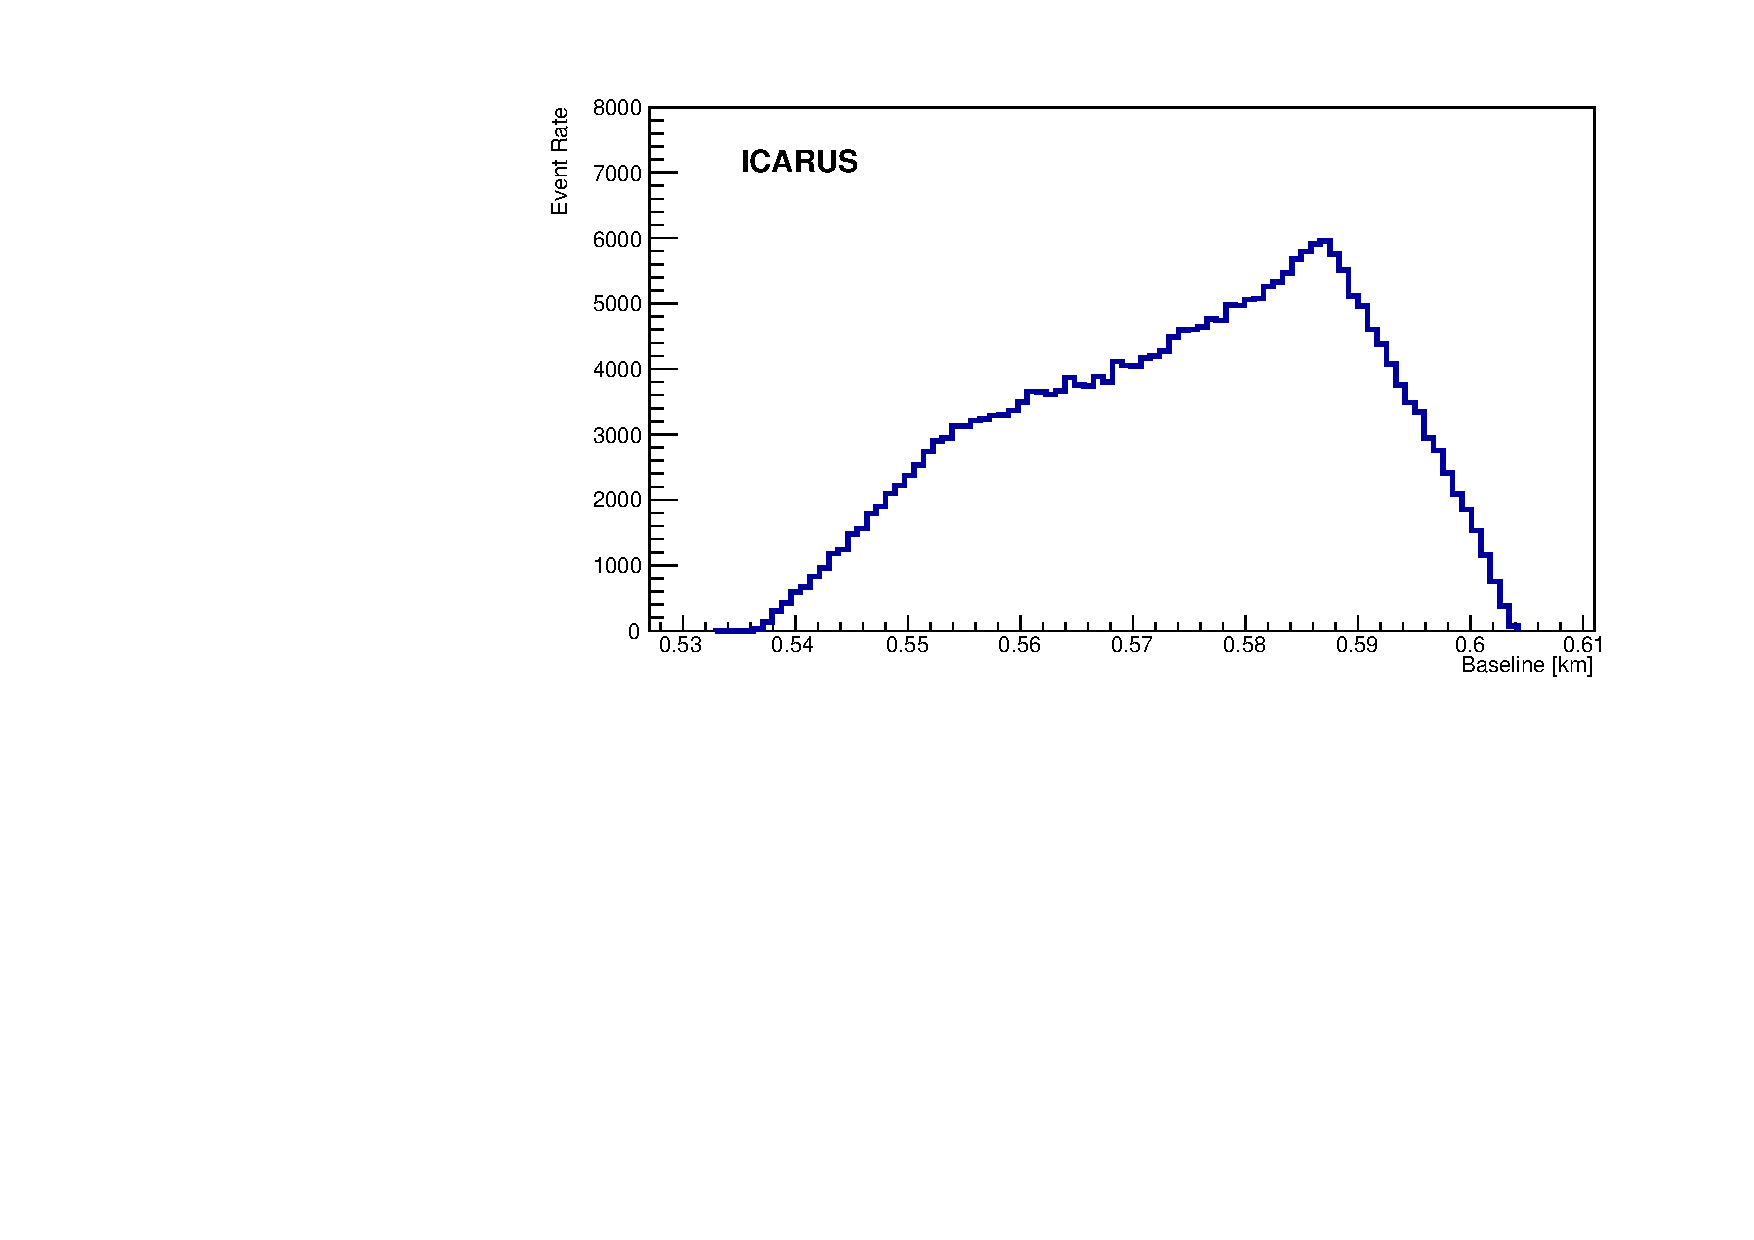
\includegraphics[width = 0.49\textwidth]{figures-chap5/ICARUS_nue.pdf}
    \captionsetup{width=0.45\textwidth}
    \parbox[b]{0.49\textwidth}%
    {
    \caption[The overall \nue baseline distributions.]{The baseline distribution of events in the overall \nue sample which is comprised of events from the intrinsic \nue, oscillated $\nu$, the \numu events from passing the \nue selection and the dirt and cosmic samples (which are not explicitly shown) for each of the \gls{sbn} detectors.}
    \label{fig:nue_baseline}
    }
\end{figure}


\newpage
\subsubsection{Binning}\label{sec:binning}
The energy binning schemes used are the same across each of the three detectors, however, the scheme used is different for the \numu and \nue analyses. Furthermore, there are separate schemes for both the true and reconstructed energies. Each of the binning schemes is outlined below. 

The \numu edge-to-edge binning has 21 bins in reconstructed neutrino energy which are bounded as follows:
\begin{itemize}
    \item One bin from 0.00 -- 0.20 GeV,
    \item Two 0.10 GeV bins from 0.20 -- 0.40 GeV,
    \item Twelve 0.05 GeV bins from 0.40 -- 1.00 GeV,
    \item Two 0.25 GeV bins from 1.00 -- 1.50 GeV,
    \item Three 0.50 GeV bins from 1.50 -- 3.00 GeV and
    \item One bin from 3.00 -- 10.00 GeV.
\end{itemize}

The \numu edge-to-edge binning has 22 bins in true neutrino energy which are bounded as follows:
\begin{itemize}
    \item One bin from 0.00 -- 0.30 GeV,
    \item Three 0.10 GeV bins from 0.30 -- 0.60 GeV,
    \item Twelve 0.05 GeV bins from 0.60 -- 1.20 GeV,
    \item One bin from 1.20 -- 1.50 GeV,
    \item Three 0.50 GeV bins from 1.50 -- 3.00 GeV,
    \item One bin from 3.00 -- 5.00 GeV and
    \item One bin from 5.00 -- 10.00 GeV.
\end{itemize}

The \nue edge-to-edge binning has 12 bins in reconstructed neutrino energy which are bounded as follows:
\begin{itemize}
    \item One bin from 0.00 -- 0.35 GeV,
    \item Five 0.15 GeV bins from 0.35 -- 1.10 GeV,
    \item Two 0.20 GeV bins from 1.10 -- 1.50 GeV,
    \item Two 0.25 GeV bins from 1.50 -- 2.00 GeV,
    \item One bin from 2.00 -- 3.00 GeV and
    \item One bin from 3.00 -- 10.00 GeV.
\end{itemize}

The \nue edge-to-edge binning has 33 bins in true neutrino energy which are bounded as follows:
\begin{itemize}
    \item Two 0.25 GeV bin from 0.00 -- 0.50 GeV,
    \item Fifteen 0.05 GeV bins from 0.50 -- 1.25 GeV,
    \item Fifteen 0.25 GeV bins from 1.25 -- 5.00 GeV and
    \item One bin from 5.00 -- 10.00 GeV.
\end{itemize}

\newpage
\subsection{Reaction Modes}
The reaction modes define the topology of neutrino interactions. Categorising neutrino events is a requirement for handling systematic uncertainties since these are reaction mode dependent. The reaction modes are grouped into two sets\footnote{The \gls{cc} QE 0\pi mode is sometimes simply written as \gls{cc} QE.}: the \textit{fine} reaction modes which outline the complete list of all possible reaction modes and the \textit{coarse} reaction modes which define a broader class of interaction which encompass one or more fine reaction mode. The fine reaction modes are listed in \TableRef{table:fine_reac_modes} and are typically used at the analysis level. The coarse reaction modes used depend on the analysis channel and are listed in \TableRef{table:coarse_reac_modes}. They are usually only used when displaying data such as in a breakdown of event rate spectra since using the complete list of reaction modes would be impractical. 

% Fine reaction modes
\begin{table}[t!]
  \renewcommand{\arraystretch}{1.6}
  \begin{tabular}{>{\centering\arraybackslash}m{4cm} 
                  >{\centering\arraybackslash}m{4cm}
                  >{\centering\arraybackslash}m{4cm}}
  
    \toprule
    \multicolumn{3}{c}{\textit{Fine Reaction Modes}} \\
    $\numu$, $\numubar$ & $\nue$, $\nuebar$ & $\numu \rightarrow \nue, \numubar \rightarrow \nuebar$ \\
    \midrule
    CC QE 0\pi                     & CC QE 0\pi                    & CC QE 0\pi \\
    NC~Elastic                 & NC~Elastic                & CC 2p2h\\ 
    CC, NC 2p2h                 & CC, NC 2p2h                & CC 1$\pi^{\pm}$ \\  
    CC, NC 1$\pi^{\pm}$        & CC, NC 1$\pi^{\pm}$       & CC 1$\pi^{0}$ \\   
    CC, NC 1$\pi^{0}$          & CC, NC 1$\pi^{0}$         & CC 2$\pi^{\pm}$ \\   
    CC, NC 2$\pi^{\pm}$        & CC, NC 2$\pi^{\pm}$       & CC 2$\pi^{0}$ \\   
    CC, NC 2$\pi^{0}$          & CC, NC 2$\pi^{0}$         & CC Coh \\   
    CC, NC $\pi^{\pm}\pi^{0}$  & CC, NC $\pi^{\pm}\pi^{0}$ & Elastic Scattering \\   
    CC, NC Coh                 & CC, NC Coh                & CC Other \\  
    CC, NC Elastic Scattering  & CC+NC Elastic Scattering  \\  
    NC 1$\gamma$               & NC 1$\gamma$              \\  
    CC, NC Other               & CC, NC Other              \\  
    \hdashline
    \multicolumn{3}{c}{\textit{Cosmic \& Dirt}} \\
    \bottomrule

  \end{tabular}
  \caption[Fine Reaction Modes.]{The complete list of reaction modes considered in an \gls{sbn} analysis. The \gls{2p2h} mode is defined as having a charged lepton + 2 nucleon topology distinguishing it from the other topologies.}
  \label{table:fine_reac_modes}
\end{table}


% Coarse reaction modes
\begin{table}[t!]
  \begin{tabular}{>{\centering\arraybackslash}m{4cm} 
    >{\centering\arraybackslash}m{4cm}}
  
    \toprule
    \multicolumn{2}{c}{\textit{Coarse Reaction Modes}} \\
    \numu, \numubar & \nue, \nuebar              \\
    \midrule
    \numu CC QE 0\pi     & \nue CC QE 0\pi       \\ 
    \numu CC 2p2h        & \nue CC 2p2h          \\ 
    \numu CC 1$\pi$      & \nue CC 1$\pi$        \\ 
    \numu CC 2$\pi$      & \nue CC 2$\pi$        \\ 
    \numu CC Other       & \nue CC Other         \\ 
    \numubar CC          & \nuebar CC            \\
    \nue \& \nuebar CC & \numu CC                \\
    NC                     & \numubar CC         \\
    \textit{Cosmic}        & Oscillated \nue CC  \\
    \textit{Dirt}          & NC 0\pi             \\
                           & NC Other            \\
                           & \textit{Cosmic}     \\
                           & \textit{Dirt}       \\
    \bottomrule

  \end{tabular}
  \caption[Coarse Reaction Modes.]{The \textit{coarse} reaction modes used for both the \numu and \nue channels. These are a broader definition of the reaction modes where one or more of the \textit{fine} reaction modes listed in \TableRef{table:fine_reac_modes} would come under the umbrella of a given coarse reaction mode.}
  \label{table:coarse_reac_modes}
\end{table}

\clearpage
\subsection{Implementing and Validating SBN Systematic Uncertainties in VALOR}

The systematics that are considered as part of the current \gls{sbn} analysis have been detailed in \SectionRef{sec:syst_uncertainties}. Unless explicitly stated, efficiency uncertainties are not considered due to there currently not being a general consensus on their magnitude. 

The systematics from the \gls{genie} and \gls{microboone} reweight packages are initially in the form of weights which correspond to variations of the parameter. Systematic uncertainties in this form can not be directly used in an oscillation analysis, but must instead first be processed internally, the details of which are described below.

\subsubsection{Processing Systematic Uncertainties}\label{sec:systematic_validation}

Many \textit{universes} are simulated, each with different weights associated with each of the systematic parameters. This allows the impact of varying systematic parameters on the event rate of neutrino interactions to be observed. If the systematic parameters are uncorrelated, the weights are simply an $n \sigma$ variation which is the value used in a given universe. For correlated parameters, the weights are due to a unique variation of all the correlated parameters of a given universe. Of the systematic uncertainties associated with either the \gls{genie} or \gls{microboone} reweight packages, only the neutrino production flux uncertainties which are listed in \TableRef{table:corr_flux} are correlated. All other parameters are uncorrelated. 

Depending on whether a given systematic parameter is correlated or not, the way that it is processed within VALOR is done in two different ways. For the uncorrelated parameters, a set of associated response functions which represent the impact on the event rate that tweaking a given systematic parameter will have are constructed. For each parameter, individual response functions are constructed for each combination of \textit{d, b, s, m, r} and \textit{t}. Each response function is a 13-knot spline which nominally represents the change in event rate from parameter variations ranging from \mbox{[-3, +3]$\sigma$} in 0.5$\sigma$ intervals. The response functions are constructed by first identifying the 12 universes which have a variation closest to each of the non-zero $\sigma$ intervals and then taking the ratio of the event rate from the selected universe in a \mbox{2D (r, t)} bin to the nominal event rate in that bin. By definition there will be a knot at 0$\sigma$ with a response of 1, however, in most cases, the remaining 12 knots will not be exactly at 0.5$\sigma$ intervals. 

For the case of correlated parameters, it is not straightforward to construct response functions as was done for the uncorrelated parameters because any variations will be due to multiple parameters. These parameters are instead represented by a covariance matrix. Matrices of this type, $\mathbf{C_{ij}}$, are constructed in true parameter space such that,
\begin{equation}
  \mathbf{C_{ij}} = \frac{1}{U} \sum_{u=1}^{U} (N_{i}^{u}-N_{i}^{cv})(N_{j}^{u}-N_{j}^{cv}),
  \label{eq:covmatrix}
\end{equation}
where \textit{U} is the number of universes, $N_{i,j}^{u}$ is the event rate in universe $u$ in bin $i$ or $j$ and $N_{i,j}^{cv}$ nominal event rate in
bin $i$ or $j$.

\subsubsection{Validating Systematic Uncertainties}
In order to establish that the systematic parameters are being correctly handled within VALOR, a comparison between the event rate variations as seen by VALOR and those obtained directly from the universes is performed. This is done in two different ways; 
\begin{enumerate}
    \item Tweak the nominal spectra using the response functions within VALOR for a single systematic parameter and then compare them with the spectra that were obtained directly from the universe files.
    \item Generate N toy samples (typically 500 in order to match the total number of universes) with some set of systematic parameters randomly tweaked. The one sigma spread from all the toys is found. This is done for both VALOR and for the universe files and the results are compared. 
\end{enumerate}

As an example, the $+1\sigma$ variation for the $f_{HornCurrent}$, $f_{M_A^{CCRes}}$ and $f_{\Delta \rightarrow N \gamma}$ parameters from the \nue sample in \gls{sbnd} between the VALOR response functions and the universes are shown in \FigureRef{fig:+1sigma_variations}\footnote{The terms \textit{spline} and \textit{response function} are used interchangeably.}. A complete list of the $+3\sigma$ variation comparisons for all the uncorrelated systematic parameters in \gls{sbnd} are shown for the \nue channel in \AppendixRef{app:single_parameter_variations}. In all cases, there is either perfect agreement or differences of only up to a few tens of events. It should be noted that the event rate shown in the spectra used for validating the systematic parameters for the \nue channel is several orders of magnitude greater than the nominal event rates as seen in for example \FigureRef{fig:nominal_nue_spectra}. This is due to manually setting the oscillation parameters to $\sin^2{2\theta_{\mu e}} = 1$ and $\Delta m_{41}^2 = 100$ eV$^2$ which ensures that many of the events from the oscillated $\numu \rightarrow \nue$ sub-sample are processed which is required because the response functions are indexed by mode and therefore contributions from all the sub-samples are needed. Since oscillation and systematic effects commute, this approach is sufficient to correctly produce a complete set of response functions. In the nominal event rate spectra, the assumption is that no oscillations occur, so no events from the oscillated sample are included hence the much lower event rate. 

\begin{figure}[h!]
    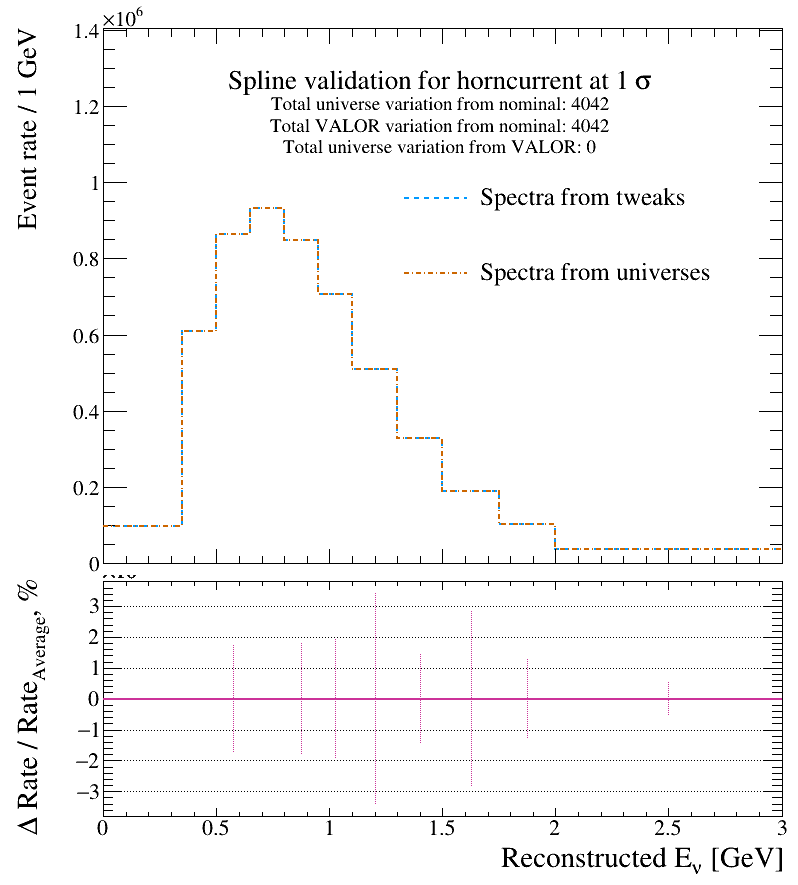
\includegraphics[width = 0.49\textwidth, height = 0.56184\textwidth]{figures-chap6/tweak_nsigma_nue/horncurrent_FluxUnisim_nuelikeCChigh_1sigma_horncurrent_FluxUnisim.png}
    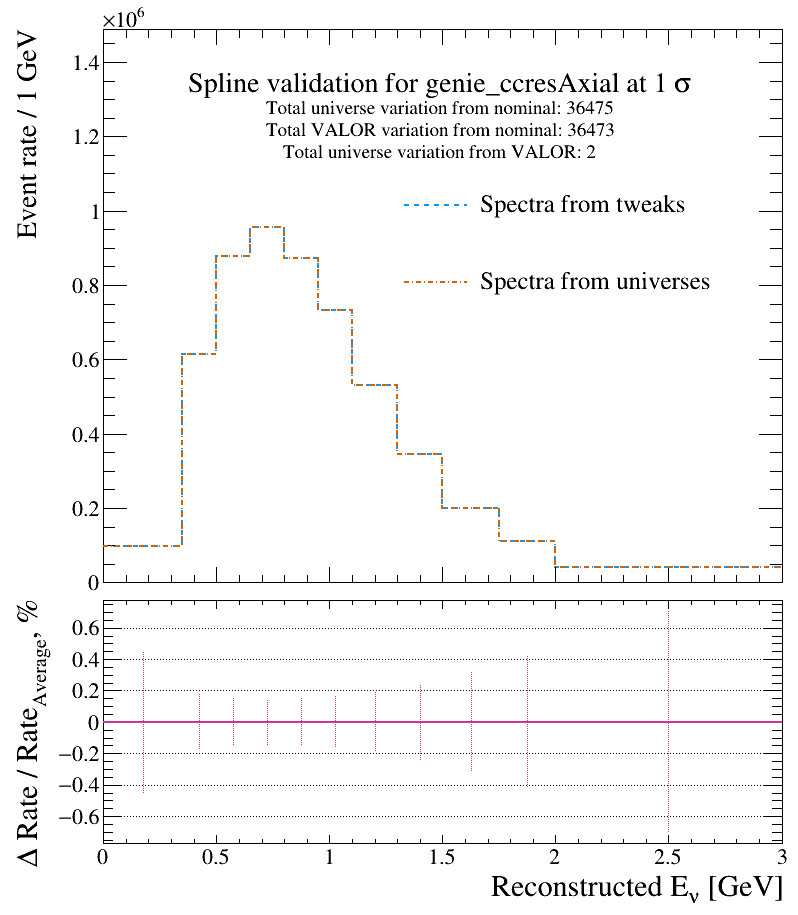
\includegraphics[width = 0.49\textwidth]{figures-chap6/tweak_nsigma_nue/genie_ccresAxial_Genie_nuelikeCChigh_1sigma_genie_ccresAxial_Genie.png}
    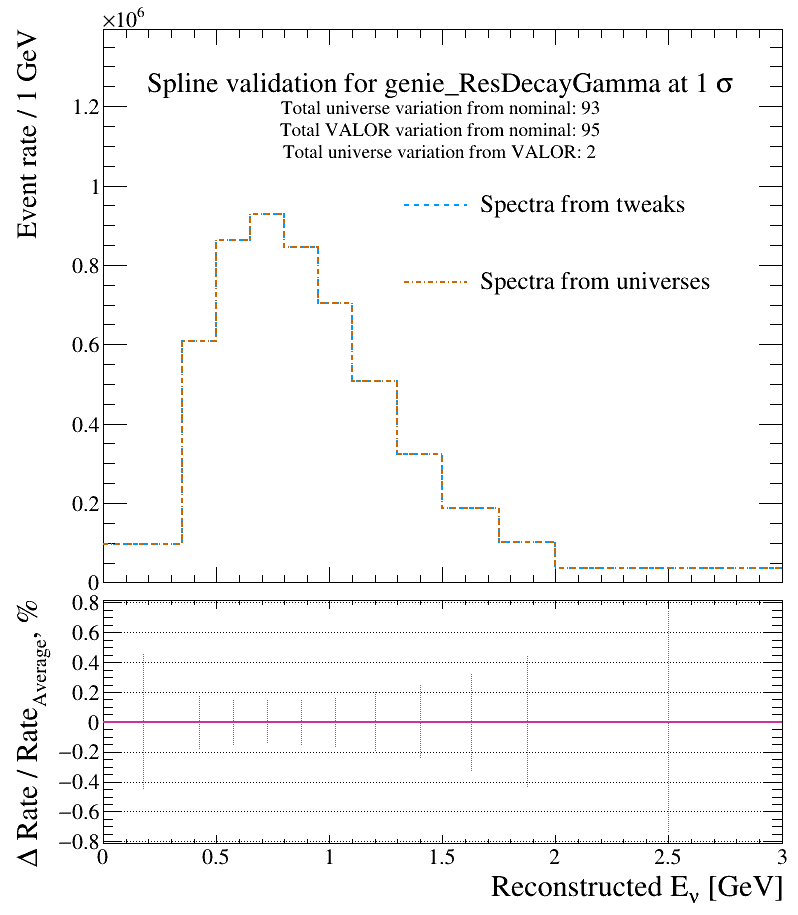
\includegraphics[width = 0.49\textwidth]{figures-chap6/tweak_nsigma_nue/genie_ResDecayGamma_Genie_nuelikeCChigh_1sigma_genie_ResDecayGamma_Genie.png}
  \captionsetup{width=0.49\textwidth}
  \parbox[b]{0.49\textwidth}%
  {
   \caption[+1$\sigma$ variation comparison for the $f_{HornCurrent}$, $f_{M_A^{CCRes}}$ and $f_{\Delta \rightarrow N \gamma}$ parameters.]{A comparison of the +1$\sigma$ variation from the response functions in VALOR and the universes for the $f_{HornCurrent}$, $f_{M_A^{CCRes}}$ and $f_{\Delta \rightarrow N \gamma}$ parameters. The $f_{HornCurrent}$ parameter shows perfect agreement between VALOR and the universes whereas both the $f_{M_A^{CCRes}}$ and $f_{\Delta \rightarrow N \gamma}$ parameters only have an event rate difference of 2. \\\phantom{.}\\
   \label{fig:+1sigma_variations}}
   }
\end{figure}

\FigureRef{fig:1sigma_variations_toys} shows a double ratio comparison from VALOR and the universes for the flux, proposal interaction and modern interaction systematic parameters. These plots are constructed by first finding the ratio between the 1$\sigma$ variation and the nominal using VALOR and the analogous ratio using the universe files. The double ratio is then constructed by taking the ratio of both the previous 1$\sigma$ ratios. There are some minor differences between the variations in VALOR and the universes, however, event-perfect agreement is not expected since the 1$\sigma$ variations are found by taking the average from many toy samples. Nevertheless, the disagreement is for the most part $< 1\%$ with a maximum of just over 2\%. 



\begin{figure}[h!]
    \begin{comment}
    Was too lazy to remake the plots and remove the label so have just overlaid a white box to hide.
    \end{comment}
    \begin{tikzpicture}
    \node at (0,0) {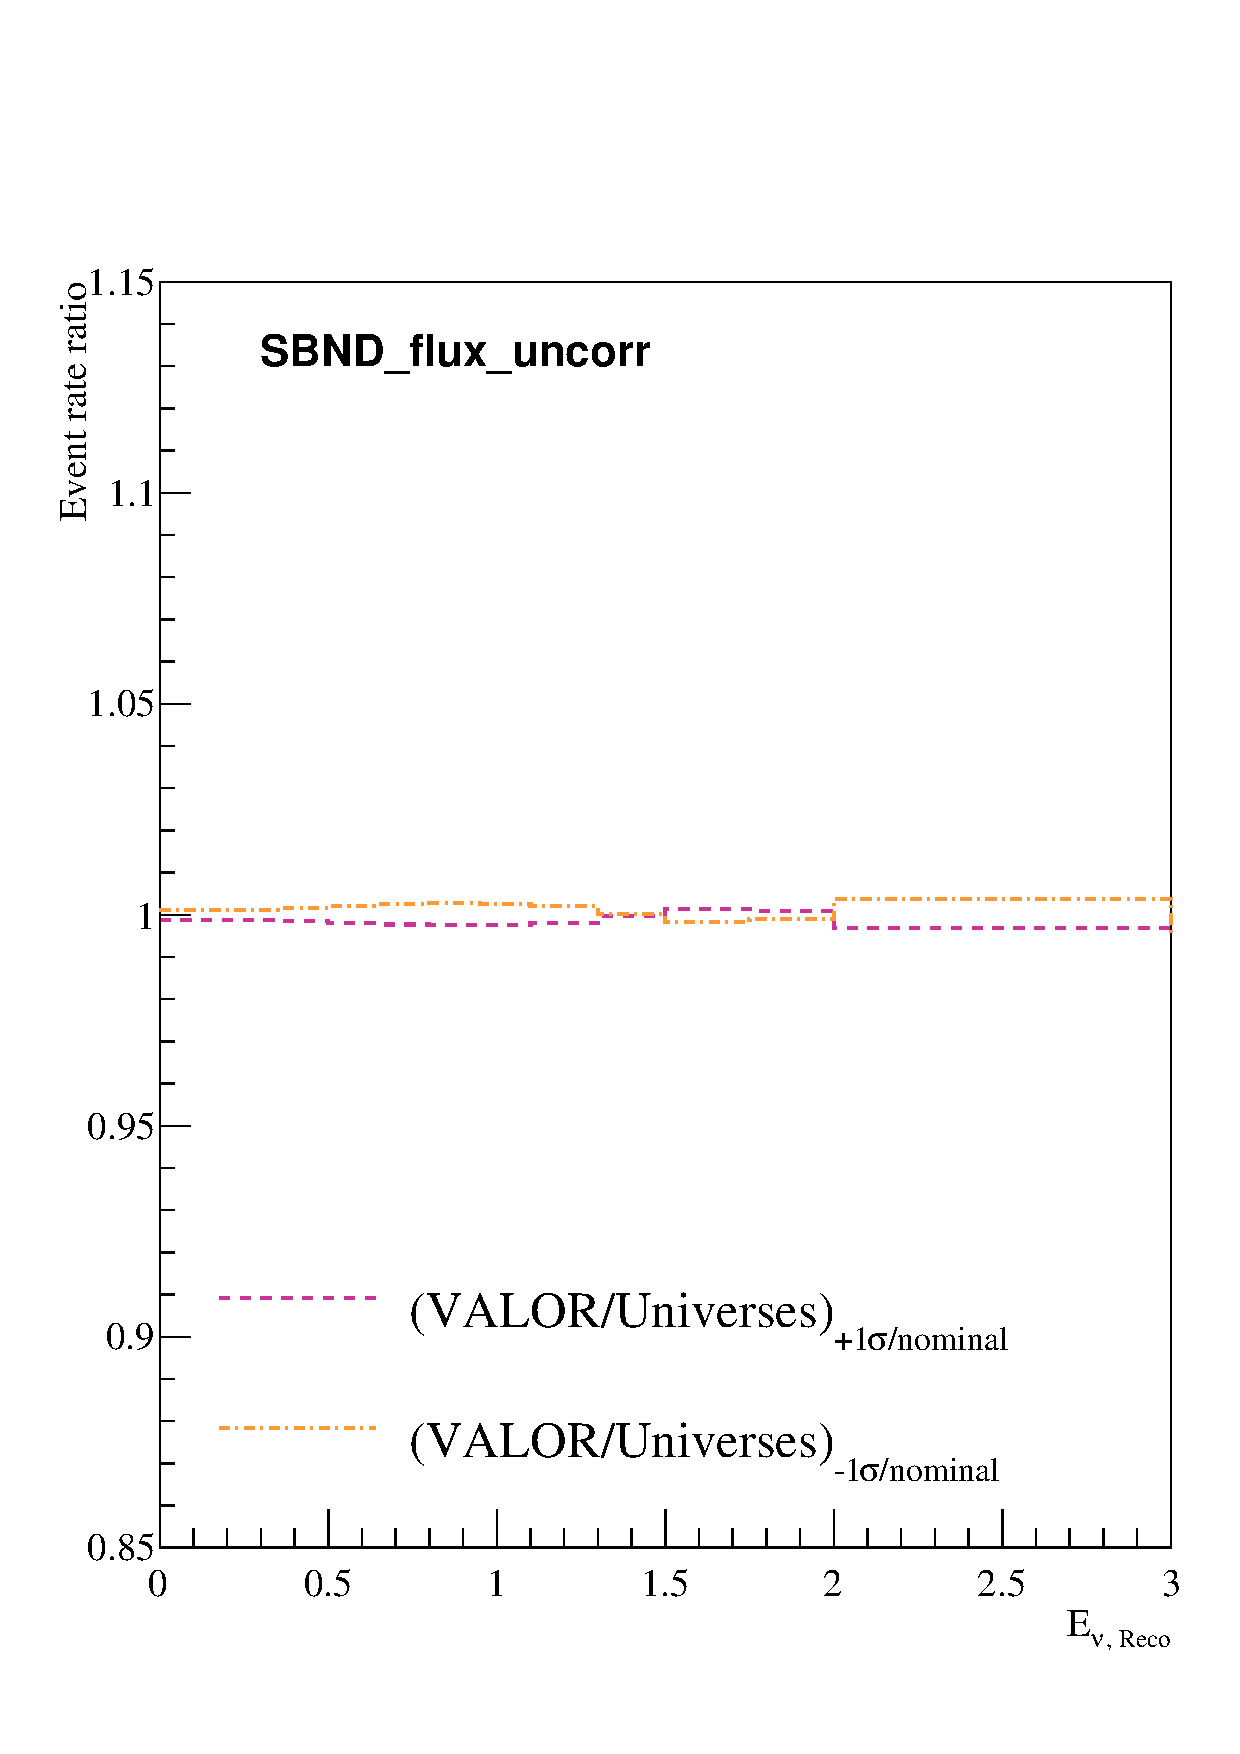
\includegraphics[width = 0.45\textwidth, height = 0.56184\textwidth]{figures-chap6/tweak_pdf_N_nue/universe_valor_double_ratios_SBND_flux_uncorr.pdf}};
    \draw [fill=white, draw=white] (-2.5,3)--(1,3)--(1,3.5)--(-2.5,3.5)--cycle;
    \draw(-1.5,3) node {Flux};
    \end{tikzpicture}
    %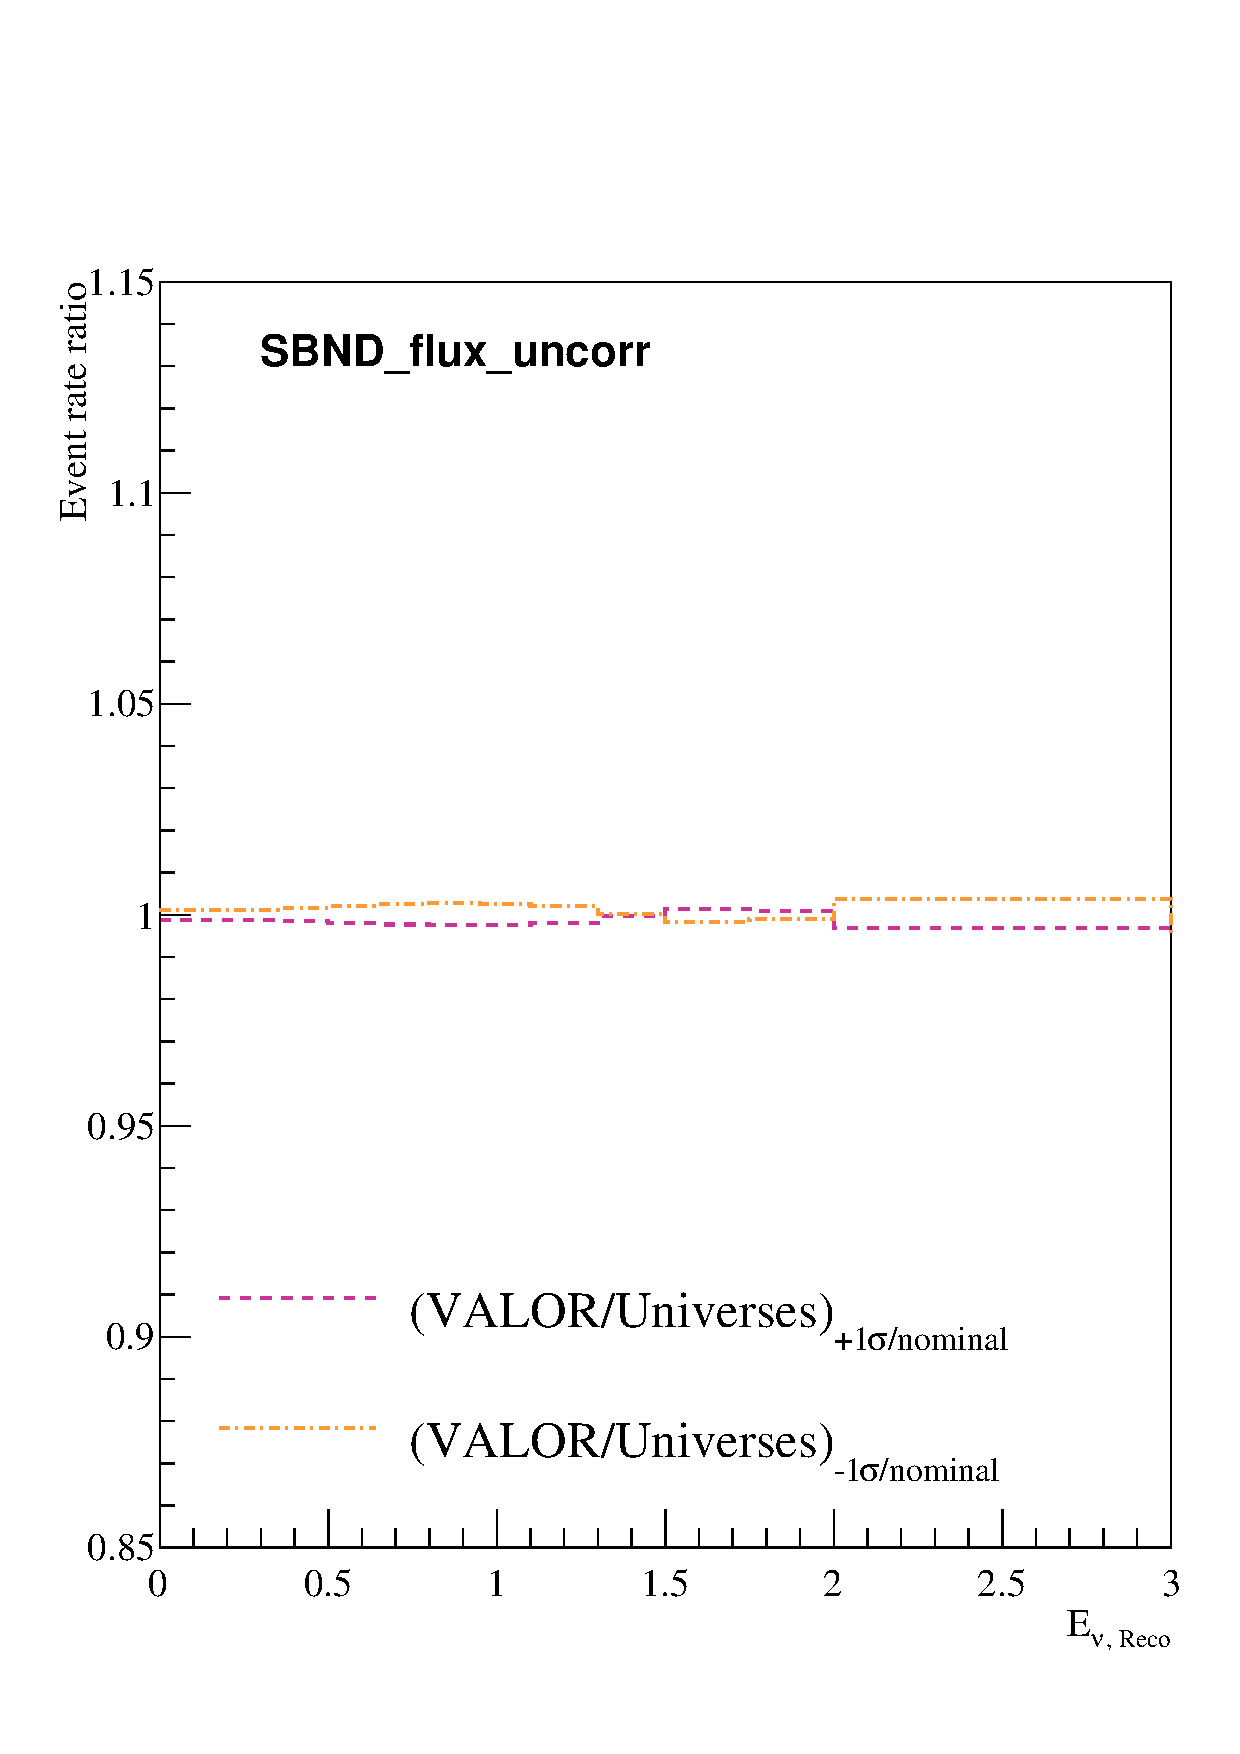
\includegraphics[width = 0.49\textwidth, height = 0.56184\textwidth]{figures-chap6/tweak_pdf_N_nue/universe_valor_double_ratios_SBND_flux_uncorr.pdf}
    \begin{tikzpicture}
    \node at (0,0) {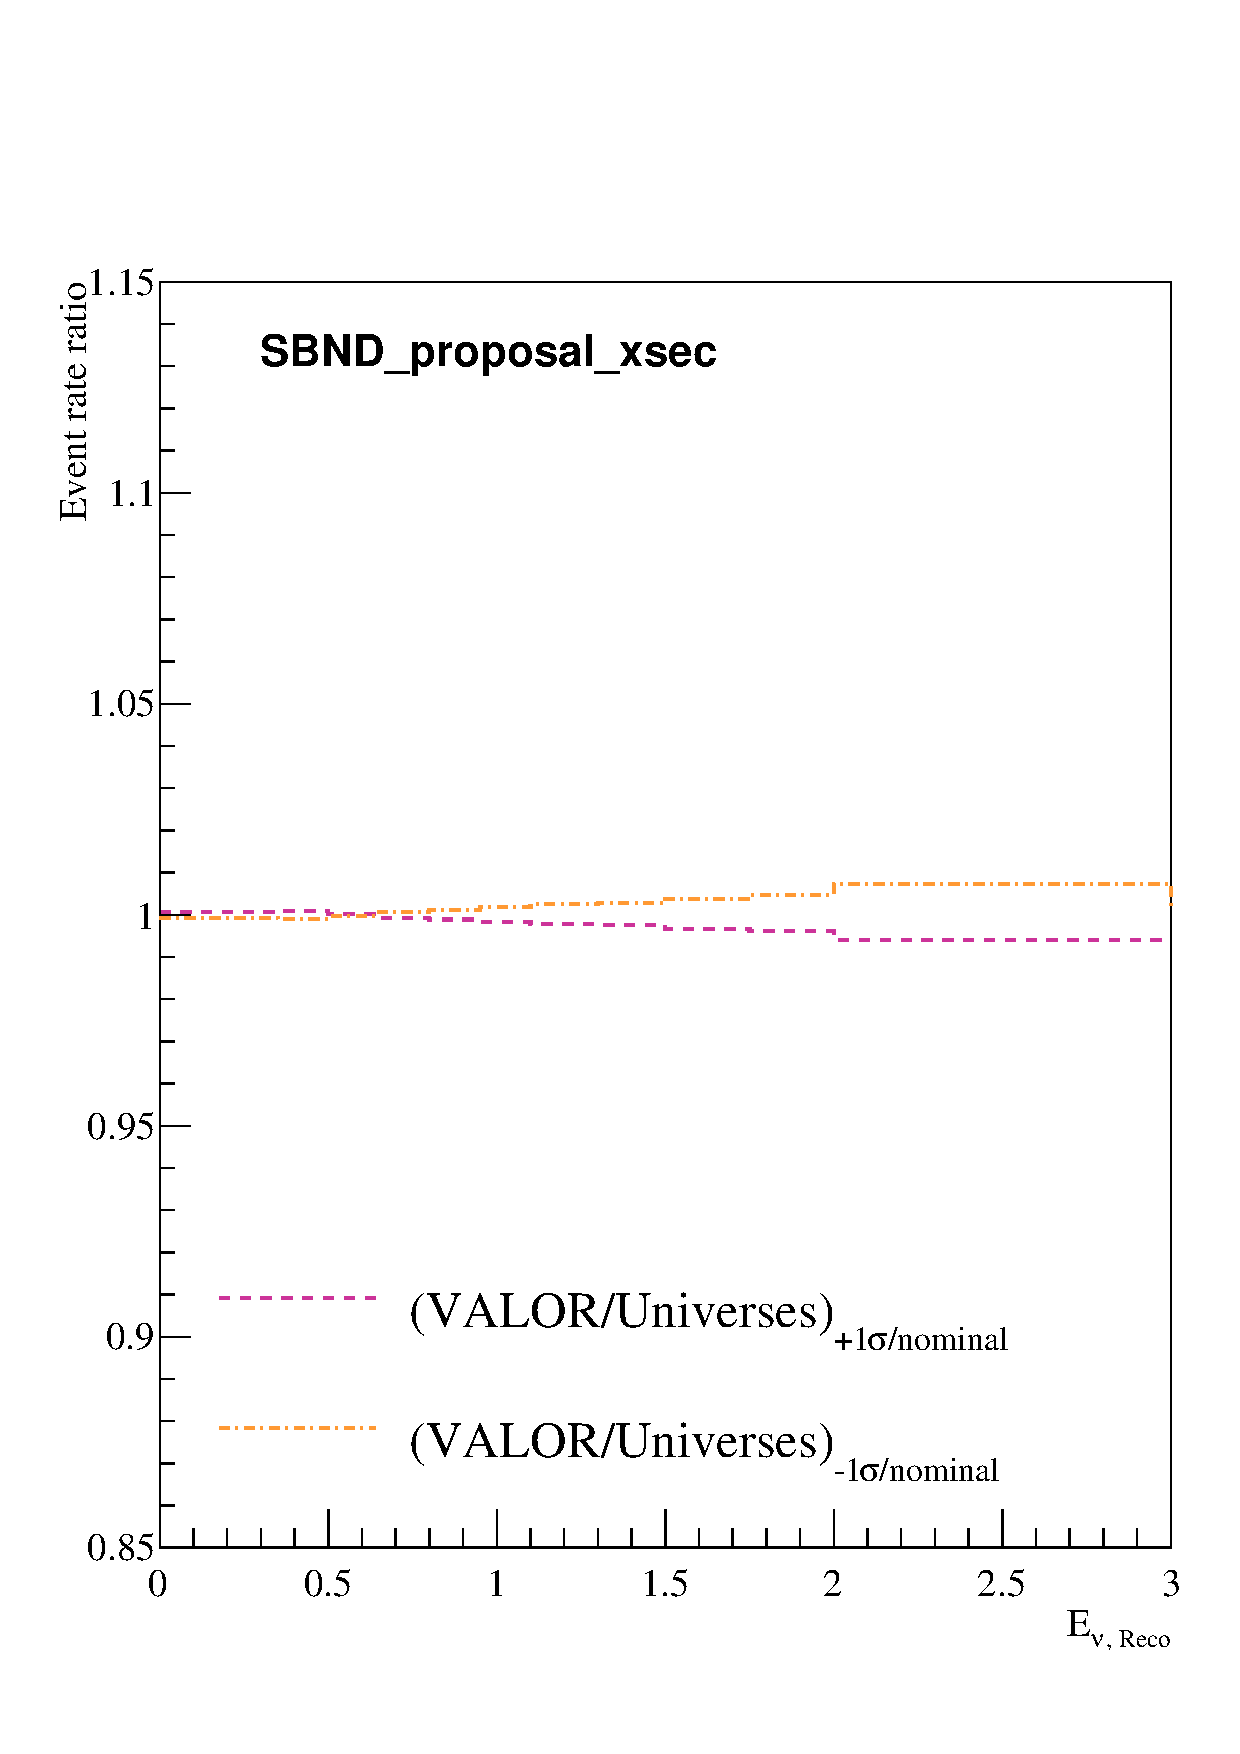
\includegraphics[width = 0.45\textwidth, height = 0.56184\textwidth]{figures-chap6/tweak_pdf_N_nue/universe_valor_double_ratios_SBND_proposal_xsec.pdf}};
    \draw [fill=white, draw=white] (-2.5,3)--(1,3)--(1,3.5)--(-2.5,3.5)--cycle;
    \draw(-0,3) node {Proposal Interaction};
    \end{tikzpicture}
    \begin{tikzpicture}
    \node at (0,0) {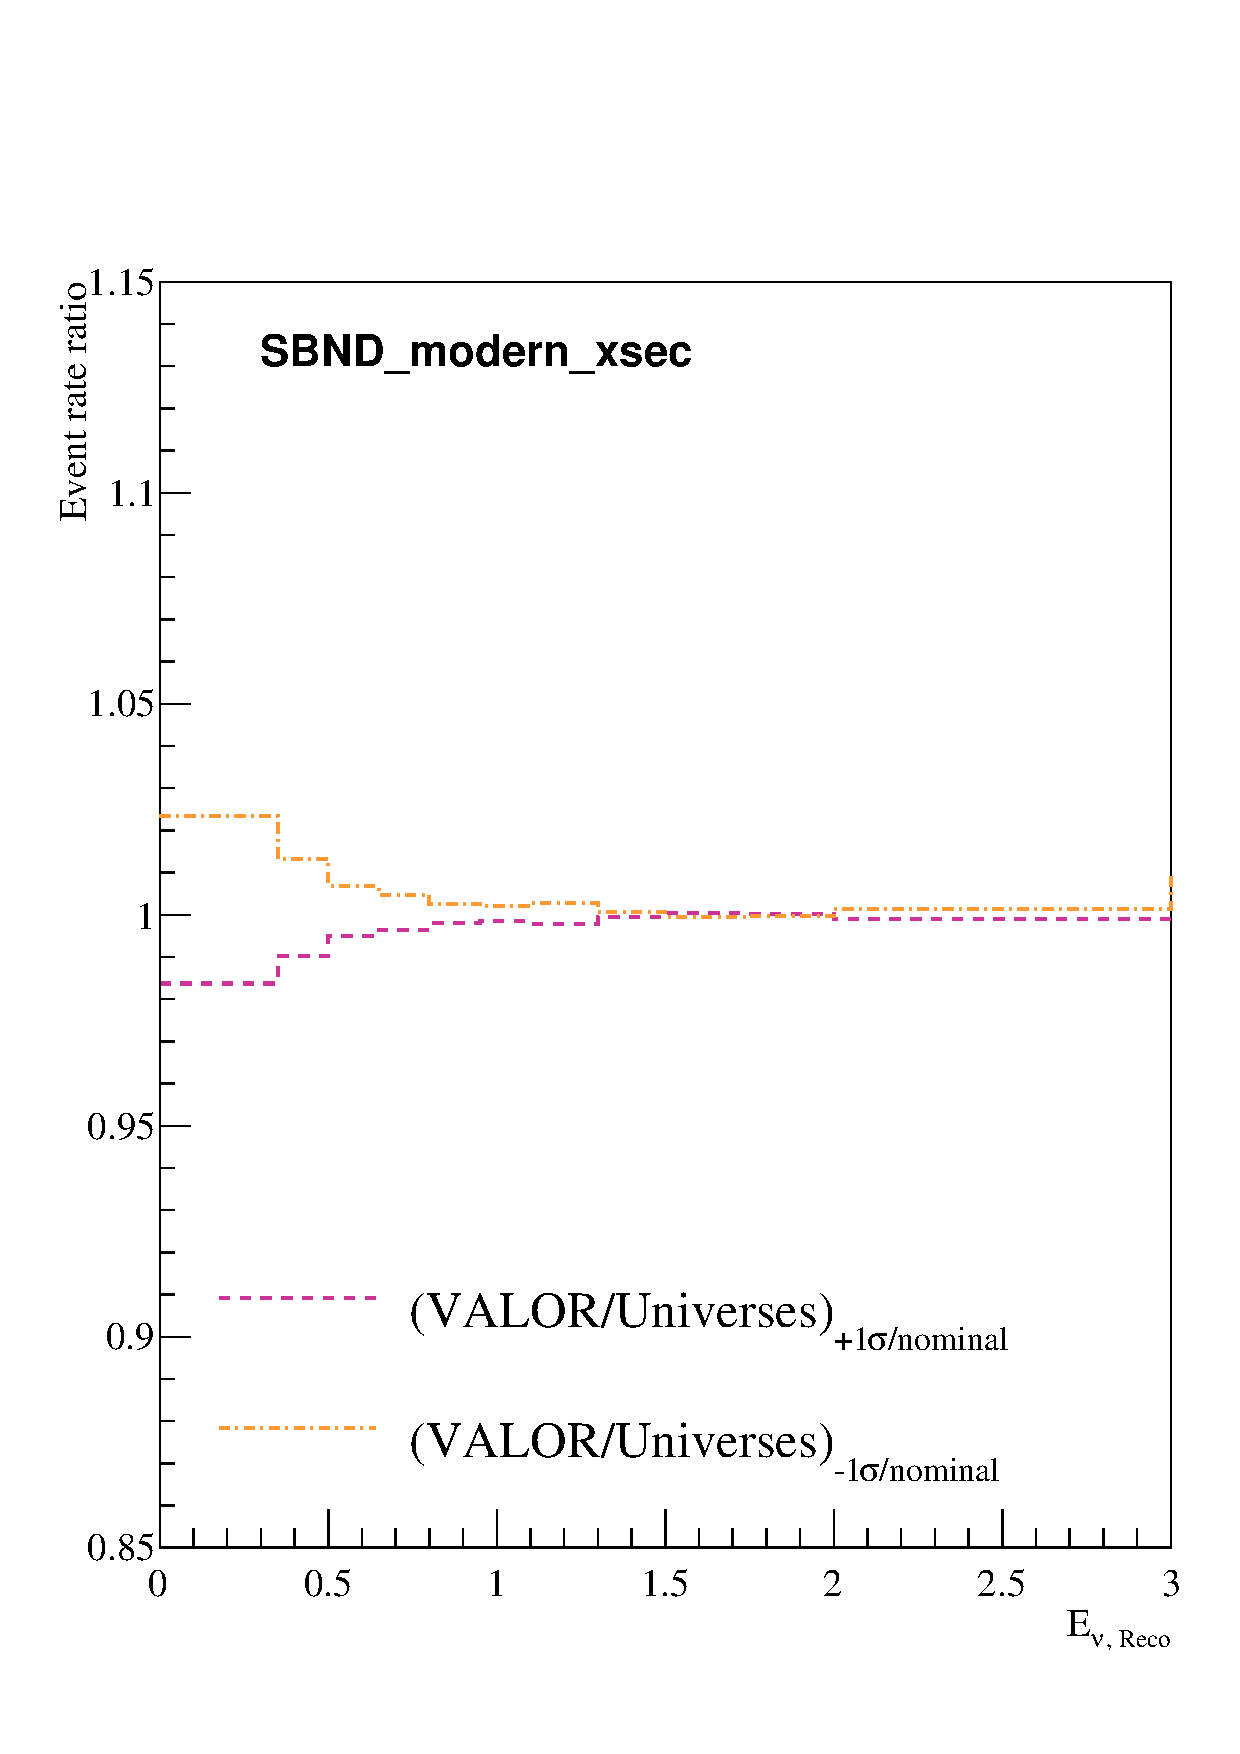
\includegraphics[width = 0.45\textwidth, height = 0.56184\textwidth]{figures-chap6/tweak_pdf_N_nue/universe_valor_double_ratios_SBND_modern_xsec.pdf}};
    \draw [fill=white, draw=white] (-2.5,3)--(1,3)--(1,3.5)--(-2.5,3.5)--cycle;
    \draw(-0,3) node {Modern Interaction};
    \end{tikzpicture}
    \vspace{0.1\textwidth}
  \captionsetup{width=0.45\textwidth}
  \parbox[b]{0.45\textwidth}%
  {
   \caption[The ratio between the $\pm 1 \sigma$ variation from VALOR and the universes for the flux, proposal interaction and modern interaction set of systematics.]{The ratio between the $\pm 1 \sigma$ variation from VALOR and the universes for the flux, proposal interaction and modern interaction set of systematic parameters.  \\\phantom{.}\\\phantom{.}\\\phantom{.}\\
   \label{fig:1sigma_variations_toys}}
  }
\end{figure}

\clearpage
\subsection{SBN Contour Construction}\label{sec:sensitivites_construction}

The relevant phase space for each of the three analysis channels considered is split into a $40 \times 40$ grid. This number was chosen in order to find a balance between having sufficient granularity when constructing contours without having excessive computing times. The dimensions of the phase space considered are different for each analysis channel and are listed in \TableRef{table:analysis_channel_phase_space}. Fits are performed for each of the $40 \times 40$ points where the oscillation parameters are fixed and the systematic parameters, if any, are allowed to float up to $\pm5\sigma$ from their nominal value. Once the fits have been produced, a contour of constant $\chi^2$ is constructed. The $\chi^2$ value is chosen such that it corresponds to a certain confidence level, \textit{CL}, which for \gls{sbn} analyses is typically 5$\sigma$. The critical value of $\chi^2$, $\chi^2_{critical}$, corresponding to a 5$\sigma$ confidence level along with a number of other $\chi^2_{critical}$ values with their associated confidence levels which are commonly seen in literature are outlined in \TableRef{table:critical_chi2_values}. The confidence levels and $\chi^2_{critical}$ are related via $CL = \int_0^{\chi^2_{critical}} \frac{e^{-x/2}x^{u/2-1}}{2^{u/2}\Gamma(u/2)} dx$, where \textit{u} is the degrees of freedom (in this case 1) and $\Gamma$ is the Gamma function \cite{critical_chi2_book}. An example of a 2D $\chi^2$ surface with exclusion contours at 90\%, 3$\sigma$ and 5$\sigma$ confidence levels for the \nue appearance channel is shown in \FigureRef{fig:nue_app_chisq_surface}. The contours have been produced for the entire \gls{sbn} program with the inclusion of flux and interaction systematics.

\begin{table}[h!]
\begin{tabular}{lcc}
\multicolumn{1}{c}{\multirow{2}{*}{Analysis Channel}} & \multicolumn{2}{c}{Phase Space Considered} \\
\multicolumn{1}{c}{} & $\sin^2{2\theta}$ & $\Delta m_{41}^2$ \\ \hline
\numu Disappearance & $\theta_{\mu\mu}$: [10$^{-3}$ -- 1] & [10$^{-2}$ -- 10$^2$] eV$^2$ \\
\nue Appearance & $\theta_{\mu e}$: [10$^{-5}$ -- 1] & [10$^{-2}$ -- 10$^2$] eV$^2$ \\
\nue Disappearance & $\theta_{ee}$: [10$^{-2}$ -- 1] & [10$^{-2}$ -- 10$^2$] eV$^2$
\end{tabular}
\caption[The phase space considered for each of the SBN analyses.]{The phase space considered when constructing contours for each of the three oscillation channels within \gls{sbn}.}
\label{table:analysis_channel_phase_space}
\end{table}

\begin{table}[h!]
\begin{tabular}{lllllll}
 Confidence level & 68\% & 90\% & 95\% & 99\% & 3$\sigma$ & 5$\sigma$ \\ \hline
$\chi^2_{critical}$ & 0.23 & 1.64 & 2.71 & 5.41 & 7.74 & 23.66
\end{tabular}
\caption[$\chi^2_{critical}$ values for various confidence levels.]{The $\chi^2_{critical}$ values corresponding to various confidence levels which are commonly used when performing sensitivity studies.}
\label{table:critical_chi2_values}
\end{table}

\begin{figure}[h!]
    \centering
    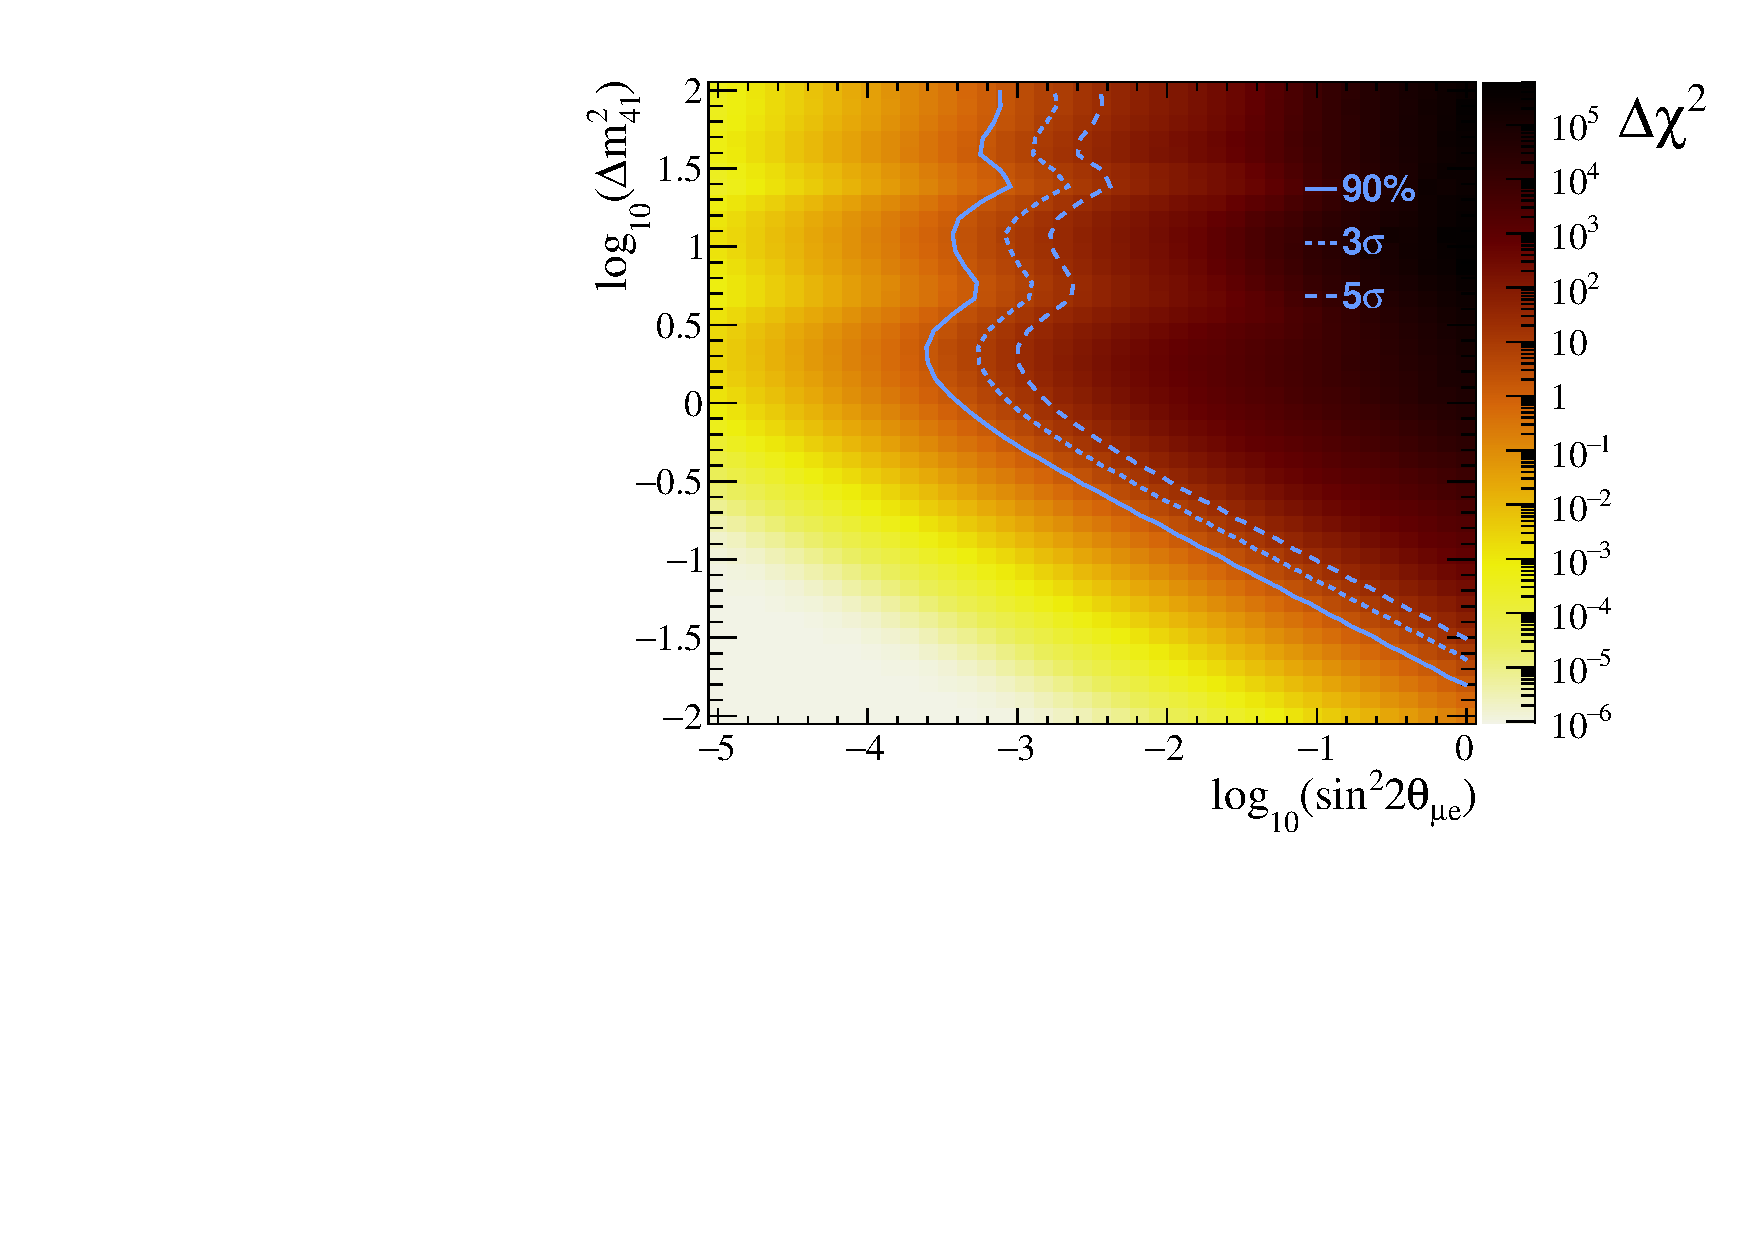
\includegraphics[width = \largefigwidth]{figures-chap6/exclusion_contours/nue_app_03d1_chi2_surface.pdf}
    \caption[\nue appearance contours overlaid on the $\chi^2$ surface.]{The \nue appearance $\chi^2$ surface from fits including flux and interaction systematics. Contours of constant $\chi^2$ values which correspond to 90\%, 3$\sigma$ and 5$\sigma$ confidence levels have been overlaid onto the surface.}
    \label{fig:nue_app_chisq_surface}
\end{figure}

\newpage

\section{Event Rate Predictions and the Expected Signal}
\begin{comment}
Event rates
Impact of systematics
Size of Signal
\end{comment}

In order to perform sensitivity calculations, the events are required to be binned in terms of a kinematical variable, which is chosen to be the reconstructed neutrino energy.

The nominal event rates, event rates with an uncertainty envelope due to systematic uncertainties and the event rates due to an oscillation signal are discussed below for each \gls{sbn} detector. Additionally, the impact of the uncorrelated systematic parameters are quantified in terms of their effect on the oscillation parameters.


\subsection{Nominal Event Rate Predictions}

It has been established that there are two oscillations channels associated with \nue: \nue appearance and \nue disappearance. Since the only difference between these channels is due to oscillations, the nominal event rates are common between the two.

The breakdown of the nominal number of events by interaction mode and channel are shown numerically in \TableRef{table:sbnd_nue_event_rate}, \TableRef{table:uboone_nue_event_rate} and \TableRef{table:icarus_nue_event_rate} for \gls{sbnd}, \gls{microboone} and \gls{icarus} respectively. The same events rates are also shown in \FigureRef{fig:nominal_nue_spectra} in the form of spectra. The spectra show the modal breakdown in terms of the coarse reaction modes where the events have been binned in reconstructed neutrino energy. 

\newpage
\begin{table}[h!]
%\section*{sbn\_nd\_\_BNB\_FHC\_\_nuelikeCChigh}
\begin{adjustbox}{width=1\textwidth}
\begin{tabular} {  l r  r  r  r  r  r  r  r  }
\hline
              & $\nu_{\mu} \rightarrow \nu_{\mu}$ & $\bar{\nu}_{\mu} \rightarrow \bar{\nu}_{\mu}$ & $\nu_{e} \rightarrow \nu_{e}$ & $\bar{\nu}_{e} \rightarrow \bar{\nu}_{e}$ & $\nu_{\mu} \rightarrow \nu_{e}$ & $\bar{\nu}_{\mu} \rightarrow \bar{\nu}_{e}$ & Non-neutrino         & Total                \\ \hline\hline
 CCQE         & 17.0                 & 0.0                  & 5957.8               & 166.6                & 0.0                  & 0.0                  & N/A                  & 6141.5               \\ \hline
 CCMEC        & 1.1                  & 0.0                  & 1433.0               & 59.7                 & 0.0                  & 0.0                  & N/A                  & 1493.8               \\ \hline
 CC1$\pi^{\pm}$ & 234.6                & 0.0                  & 2859.9               & 112.4                & 0.0                  & 0.0                  & N/A                  & 3206.8               \\ \hline
 CC1$\pi^{0}$   & 230.7                & 0.0                  & 513.8                & 14.6                 & 0.0                  & 0.0                  & N/A                  & 759.2                \\ \hline
 CC2$\pi^{\pm}$ & 19.3                 & 0.0                  & 293.3                & 7.9                  & 0.0                  & 0.0                  & N/A                  & 320.6                \\ \hline
 CC2$\pi^{0}$   & 5.2                  & 0.0                  & 24.1                 & 0.6                  & 0.0                  & 0.0                  & N/A                  & 29.9                 \\ \hline
 CC1$\pi^{0}1\pi^{\pm}$ & 37.1                 & 0.0                  & 187.0                & 7.0                  & 0.0                  & 0.0                  & N/A                  & 231.1                \\ \hline
 CCcoherent   & 0.0                  & 0.0                  & 38.1                 & 3.8                  & 0.0                  & 0.0                  & N/A                  & 41.9                 \\ \hline
 CC\nue\text{El} & 0.0                  & 0.0                  & N/A                  & N/A                  & N/A                  & N/A                  & N/A                  & 0.0                  \\ \hline
 CCother      & 20.7                 & 0.0                  & 270.9                & 8.3                  & 0.0                  & 0.0                  & N/A                  & 299.9                \\ \hline
 NCEL         & 3.4                  & 0.0                  & 0.0                  & 0.0                  & N/A                  & N/A                  & N/A                  & 3.5                  \\ \hline
 NCMEC        & 0.6                  & 0.0                  & 0.0                  & 0.0                  & N/A                  & N/A                  & N/A                  & 0.6                  \\ \hline
 NC1$\pi^{\pm}$ & 135.6                & 0.0                  & 0.8                  & 0.0                  & N/A                  & N/A                  & N/A                  & 136.4                \\ \hline
 NC1$\pi^{0}$   & 772.6                & 0.0                  & 5.5                  & 0.2                  & N/A                  & N/A                  & N/A                  & 778.4                \\ \hline
 NC2$\pi^{\pm}$ & 2.3                  & 0.0                  & 0.1                  & 0.0                  & N/A                  & N/A                  & N/A                  & 2.4                  \\ \hline
 NC2$\pi^{0}$   & 6.9                  & 0.0                  & 0.1                  & 0.0                  & N/A                  & N/A                  & N/A                  & 7.0                  \\ \hline
 NC1$\pi^{0}1\pi^{\pm}$ & 16.1                 & 0.0                  & 0.4                  & 0.0                  & N/A                  & N/A                  & N/A                  & 16.5                 \\ \hline
 NCcoherent   & 76.8                 & 0.0                  & 0.4                  & 0.1                  & N/A                  & N/A                  & N/A                  & 77.2                 \\ \hline
 NC1$\gamma$    & 0.0                  & 0.0                  & 0.0                  & 0.0                  & N/A                  & N/A                  & N/A                  & 0.0                  \\ \hline
 NC\nue\text{El} & 181.9                & 0.0                  & N/A                  & N/A                  & N/A                  & N/A                  & N/A                  & 181.9                \\ \hline
 NCother      & 50.0                 & 0.0                  & 0.5                  & 0.0                  & N/A                  & N/A                  & N/A                  & 50.5                 \\ \hline
 \nue\text{El} & N/A                  & N/A                  & 0.0                  & 0.0                  & 0.0                  & 0.0                  & N/A                  & 0.0                  \\ \hline
 cosmic       & N/A                  & N/A                  & N/A                  & N/A                  & N/A                  & N/A                  & 0.3                  & 0.3                  \\ \hline
 dirt         & N/A                  & N/A                  & N/A                  & N/A                  & N/A                  & N/A                  & 33.9                 & 33.9                 \\ \hline
\hline
 Total        & 1812.0               & 0.0                  & 11585.9              & 381.3                & 0.0                  & 0.0                  & 34.2                 & 13813.5              \\ \hline


\end{tabular}
\end{adjustbox}

%\noindent Total: 13813.452    (13813.452) \newline
%POT: 6.600E20
\caption[Nominal \nue event rate breakdown in \gls{sbnd}.]{Nominal \nue event rate breakdown in \gls{sbnd}.}
\label{table:sbnd_nue_event_rate}
\end{table}


\newpage
\begin{table}[h!]
%\section*{sbn\_uboone\_\_BNB\_FHC\_\_nuelikeCChigh}
\begin{adjustbox}{width=1\textwidth}
\begin{tabular} {l r r r r r r r r}
\hline

              & $\nu_{\mu} \rightarrow \nu_{\mu}$ & $\bar{\nu}_{\mu} \rightarrow \bar{\nu}_{\mu}$ & $\nu_{e} \rightarrow \nu_{e}$ & $\bar{\nu}_{e} \rightarrow \bar{\nu}_{e}$ & $\nu_{\mu} \rightarrow \nu_{e}$ & $\bar{\nu}_{\mu} \rightarrow \bar{\nu}_{e}$ & Non-neutrino         & Total                \\ \hline\hline
 CCQE         & 4.2                  & 0.0                  & 384.9                & 10.4                 & 0.0                  & 0.0                  & N/A                  & 399.5                \\ \hline
 CCMEC        & 0.1                  & 0.0                  & 93.9                 & 3.7                  & 0.0                  & 0.0                  & N/A                  & 97.6                 \\ \hline
 CC1$\pi^{\pm}$ & 18.9                 & 0.0                  & 196.8                & 7.5                  & 0.0                  & 0.0                  & N/A                  & 223.2                \\ \hline
 CC1$\pi^{0}$   & 19.1                 & 1.0                  & 35.5                 & 1.1                  & 0.0                  & 0.0                  & N/A                  & 56.7                 \\ \hline
 CC2$\pi^{\pm}$ & 1.0                  & 0.0                  & 21.9                 & 0.6                  & 0.0                  & 0.0                  & N/A                  & 23.5                 \\ \hline
 CC2$\pi^{0}$   & 3.3                  & 0.0                  & 1.9                  & 0.1                  & 0.0                  & 0.0                  & N/A                  & 5.2                  \\ \hline
 CC1$\pi^{0}1\pi^{\pm}$ & 7.2                  & 0.0                  & 13.6                 & 0.6                  & 0.0                  & 0.0                  & N/A                  & 21.4                 \\ \hline
 CCcoherent   & 0.0                  & 0.0                  & 2.6                  & 0.4                  & 0.0                  & 0.0                  & N/A                  & 3.0                  \\ \hline
 CC\nue\text{El} & 0.0                  & 0.0                  & N/A                  & N/A                  & N/A                  & N/A                  & N/A                  & 0.0                  \\ \hline
 CCother      & 3.3                  & 0.0                  & 19.1                 & 0.4                  & 0.0                  & 0.0                  & N/A                  & 22.9                 \\ \hline
 NCEL         & 0.3                  & 0.0                  & 0.0                  & 0.0                  & N/A                  & N/A                  & N/A                  & 0.3                  \\ \hline
 NCMEC        & 0.0                  & 0.0                  & 0.0                  & 0.0                  & N/A                  & N/A                  & N/A                  & 0.0                  \\ \hline
 NC1$\pi^{\pm}$ & 13.9                 & 0.0                  & 0.1                  & 0.0                  & N/A                  & N/A                  & N/A                  & 14.0                 \\ \hline
 NC1$\pi^{0}$   & 59.3                 & 1.0                  & 0.4                  & 0.0                  & N/A                  & N/A                  & N/A                  & 60.7                 \\ \hline
 NC2$\pi^{\pm}$ & 0.7                  & 0.0                  & 0.0                  & 0.0                  & N/A                  & N/A                  & N/A                  & 0.7                  \\ \hline
 NC2$\pi^{0}$   & 0.7                  & 0.1                  & 0.0                  & 0.0                  & N/A                  & N/A                  & N/A                  & 0.7                  \\ \hline
 NC1$\pi^{0}1\pi^{\pm}$ & 2.3                  & 0.0                  & 0.0                  & 0.0                  & N/A                  & N/A                  & N/A                  & 2.3                  \\ \hline
 NCcoherent   & 5.5                  & 0.2                  & 0.0                  & 0.0                  & N/A                  & N/A                  & N/A                  & 5.8                  \\ \hline
 NC1$\gamma$    & 0.0                  & 0.0                  & 0.0                  & 0.0                  & N/A                  & N/A                  & N/A                  & 0.0                  \\ \hline
 NC\nue\text{El} & 14.9                 & 0.0                  & N/A                  & N/A                  & N/A                  & N/A                  & N/A                  & 14.9                 \\ \hline
 NCother      & 3.3                  & 0.0                  & 0.0                  & 0.0                  & N/A                  & N/A                  & N/A                  & 3.3                  \\ \hline
 \nue\text{El} & N/A                  & N/A                  & 0.0                  & 0.0                  & 0.0                  & 0.0                  & N/A                  & 0.0                  \\ \hline
 cosmic       & N/A                  & N/A                  & N/A                  & N/A                  & N/A                  & N/A                  & 0.0                  & 0.0                  \\ \hline
 dirt         & N/A                  & N/A                  & N/A                  & N/A                  & N/A                  & N/A                  & 14.8                 & 14.8                 \\ \hline
\hline
Total        & 157.8                & 2.3                  & 770.9                & 24.8                 & 0.0                  & 0.0                  & 14.8                 & 970.6            

       \\ \hline

\end{tabular}
\end{adjustbox}

%\noindent Total: 970.564    (970.564) \newline
%POT: 13.200E20
\caption[Nominal \nue event rate breakdown in \gls{microboone}.]{Nominal \nue event rate breakdown in \gls{microboone}.}
\label{table:uboone_nue_event_rate}
\end{table}


\newpage
\begin{table}[h!]
%\section*{sbn\_icarus\_\_BNB\_FHC\_\_nuelikeCChigh}
\begin{adjustbox}{width=1\textwidth}
\begin{tabular} {l r r r r r r r r}
\hline

              & $\nu_{\mu} \rightarrow \nu_{\mu}$ & $\bar{\nu}_{\mu} \rightarrow \bar{\nu}_{\mu}$ & $\nu_{e} \rightarrow \nu_{e}$ & $\bar{\nu}_{e} \rightarrow \bar{\nu}_{e}$ & $\nu_{\mu} \rightarrow \nu_{e}$ & $\bar{\nu}_{\mu} \rightarrow \bar{\nu}_{e}$ & Non-neutrino         & Total                \\ \hline\hline
 CCQE         & 4.6                  & 0.0                  & 727.9                & 19.3                 & 0.0                  & 0.0                  & N/A                  & 751.9                \\ \hline
 CCMEC        & 0.2                  & 0.0                  & 176.5                & 7.1                  & 0.0                  & 0.0                  & N/A                  & 183.8                \\ \hline
 CC1$\pi^{\pm}$ & 37.4                 & 0.2                  & 372.3                & 12.9                 & 0.0                  & 0.0                  & N/A                  & 422.8                \\ \hline
 CC1$\pi^{0}$   & 25.8                 & 0.1                  & 64.8                 & 2.2                  & 0.0                  & 0.0                  & N/A                  & 92.9                 \\ \hline
 CC2$\pi^{\pm}$ & 4.9                  & 0.1                  & 39.4                 & 1.0                  & 0.0                  & 0.0                  & N/A                  & 45.4                 \\ \hline
 CC2$\pi^{0}$   & 2.9                  & 0.1                  & 3.6                  & 0.1                  & 0.0                  & 0.0                  & N/A                  & 6.6                  \\ \hline
 CC1$\pi^{0}1\pi^{\pm}$ & 7.5                  & 0.0                  & 25.8                 & 1.1                  & 0.0                  & 0.0                  & N/A                  & 34.5                 \\ \hline
 CCcoherent   & 0.0                  & 0.0                  & 5.0                  & 0.5                  & 0.0                  & 0.0                  & N/A                  & 5.4                  \\ \hline
 CC\nue\text{El} & 0.0                  & 0.0                  & N/A                  & N/A                  & N/A                  & N/A                  & N/A                  & 0.0                  \\ \hline
 CCother      & 2.8                  & 0.0                  & 36.9                 & 0.8                  & 0.0                  & 0.0                  & N/A                  & 40.5                 \\ \hline
 NCEL         & 0.5                  & 0.0                  & 0.0                  & 0.0                  & N/A                  & N/A                  & N/A                  & 0.5                  \\ \hline
 NCMEC        & 0.0                  & 0.0                  & 0.0                  & 0.0                  & N/A                  & N/A                  & N/A                  & 0.0                  \\ \hline
 NC1$\pi^{\pm}$ & 17.7                 & 0.2                  & 0.1                  & 0.0                  & N/A                  & N/A                  & N/A                  & 18.1                 \\ \hline
 NC1$\pi^{0}$   & 108.5                & 0.7                  & 0.7                  & 0.0                  & N/A                  & N/A                  & N/A                  & 110.0                \\ \hline
 NC2$\pi^{\pm}$ & 0.7                  & 0.0                  & 0.0                  & 0.0                  & N/A                  & N/A                  & N/A                  & 0.8                  \\ \hline
 NC2$\pi^{0}$   & 0.9                  & 0.0                  & 0.0                  & 0.0                  & N/A                  & N/A                  & N/A                  & 0.9                  \\ \hline
 NC1$\pi^{0}1\pi^{\pm}$ & 3.4                  & 0.1                  & 0.1                  & 0.0                  & N/A                  & N/A                  & N/A                  & 3.6                  \\ \hline
 NCcoherent   & 11.3                 & 0.4                  & 0.1                  & 0.0                  & N/A                  & N/A                  & N/A                  & 11.8                 \\ \hline
 NC1$\gamma$    & 0.0                  & 0.0                  & 0.0                  & 0.0                  & N/A                  & N/A                  & N/A                  & 0.0                  \\ \hline
 NC\nue\text{El} & 17.9                 & 0.0                  & N/A                  & N/A                  & N/A                  & N/A                  & N/A                  & 17.9                 \\ \hline
 NCother      & 8.0                  & 0.0                  & 0.1                  & 0.0                  & N/A                  & N/A                  & N/A                  & 8.1                  \\ \hline
 \nue\text{El} & N/A                  & N/A                  & 0.0                  & 0.0                  & 0.0                  & 0.0                  & N/A                  & 0.0                  \\ \hline
 cosmic       & N/A                  & N/A                  & N/A                  & N/A                  & N/A                  & N/A                  & 2.3                  & 2.3                  \\ \hline
 dirt         & N/A                  & N/A                  & N/A                  & N/A                  & N/A                  & N/A                  & 24.1                 & 24.1                 \\ \hline
\hline
 Total        & 255.0                & 2.0                  & 1453.3               & 44.9                 & 0.0                  & 0.0                  & 26.4                 & 1781.6       

 \\ \hline

\end{tabular}
\end{adjustbox}

%\noindent Total: 1781.637    (1781.637) \newline
%POT: 6.600E20
\caption[Nominal \nue event rate breakdown in \gls{icarus}.]{Nominal \nue event rate breakdown in \gls{icarus}.}
\label{table:icarus_nue_event_rate}
\end{table}

\newpage
Similar to \FigureRef{fig:nominal_nue_spectra}, \FigureRef{fig:nominal_nue_spectra_1sigma_enevelope} again shows the nominal event rate in each \gls{sbn} detector, but in an integrated form. Additionally, $1\sigma$ prefit uncertainty envelopes are shown which are due to the flux and interaction systematics. The accuracy of say the \gls{icarus} prediction can be improved by constraining the systematics from an \gls{sbnd} fit. This is shown in \FigureRef{fig:icarus_pre_post_fit} which shows the nominal integrated \gls{icarus} spectrum along with the prefit uncertainty envelope as in \FigureRef{fig:nominal_nue_spectra_1sigma_enevelope}, but also a postfit uncertainty envelope based on an \gls{sbnd} fit is shown. The reduction in size from the prefit to postfit envelope highlights the impact of \gls{sbnd} on the \gls{icarus} prediction. 

\begin{figure}[h!]
  {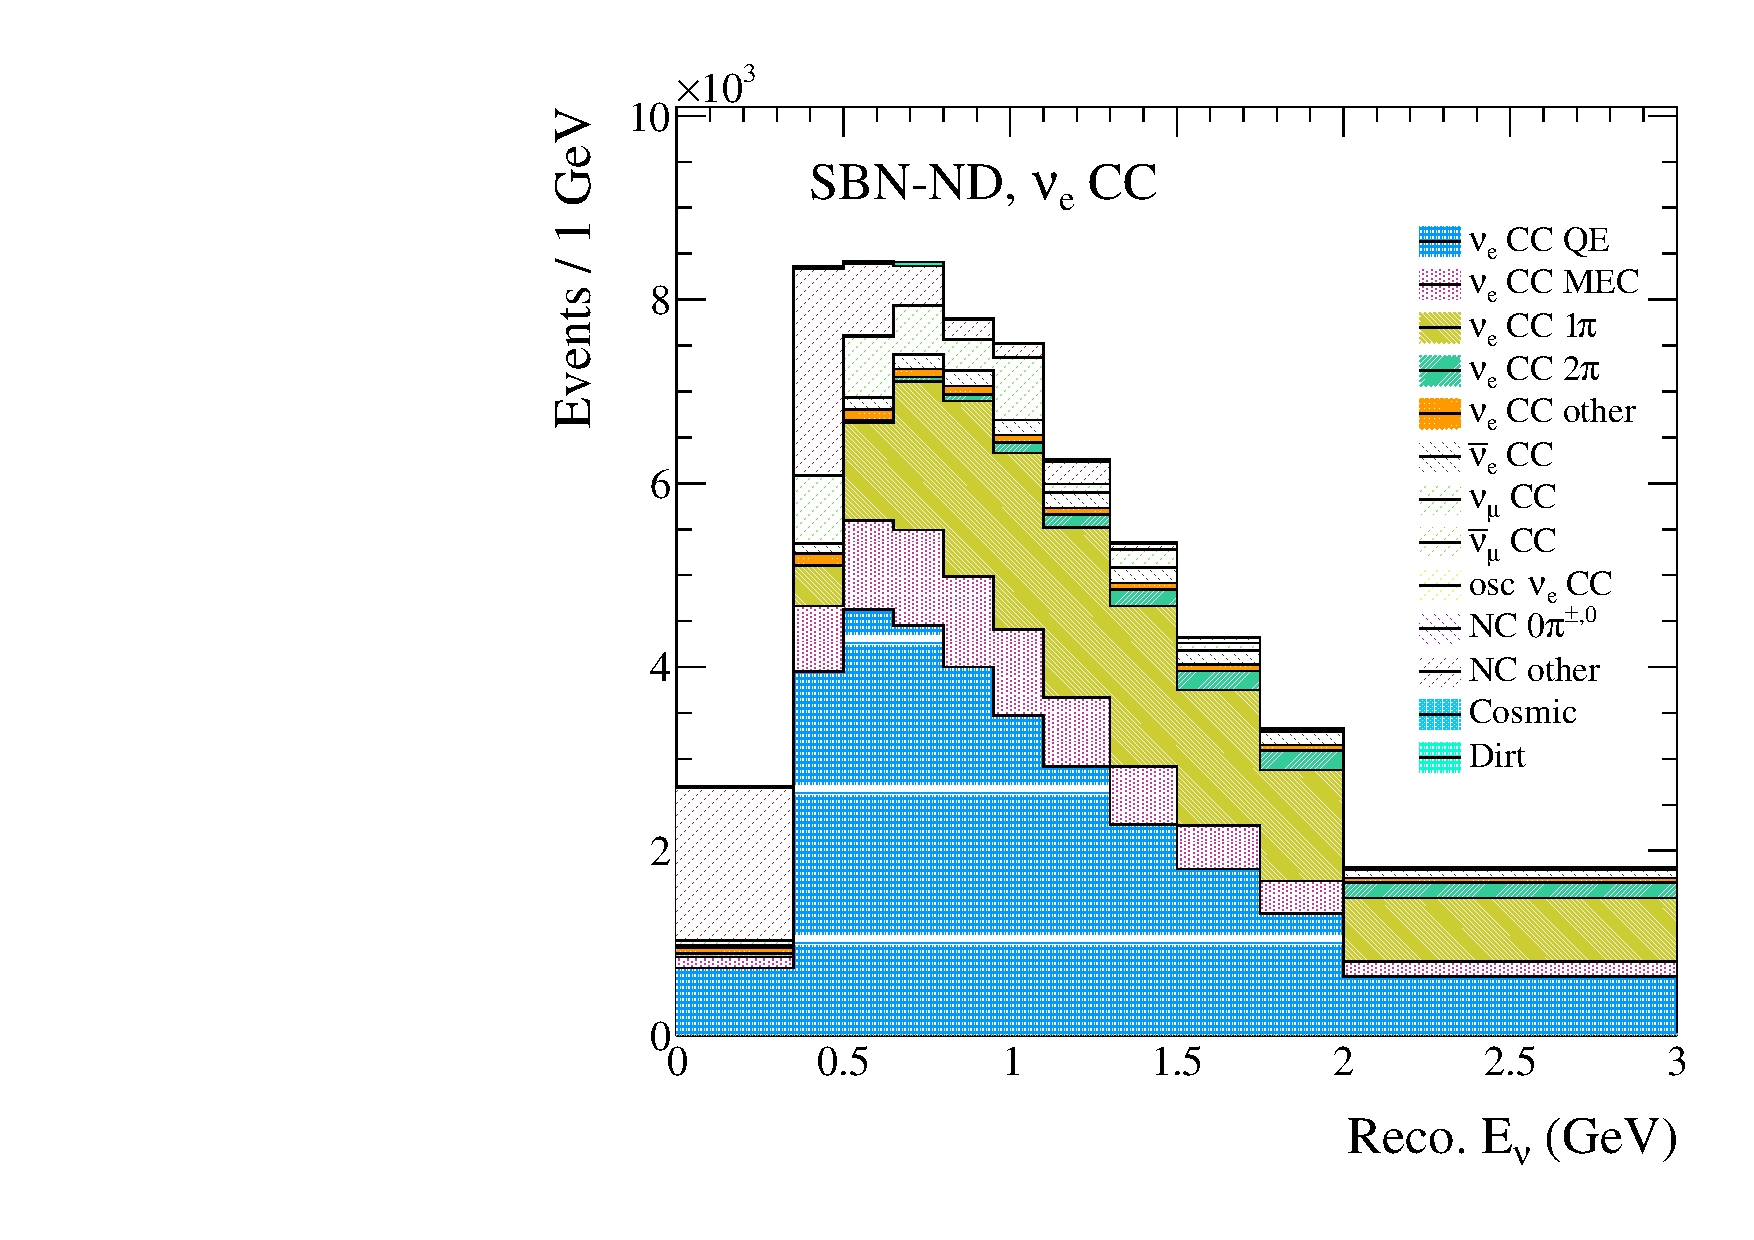
\includegraphics[width=0.49\textwidth]{figures-chap6/spectra/nue_nominal_spectrum_sbn_nd_BNB_FHC_0_modes.pdf}}
  {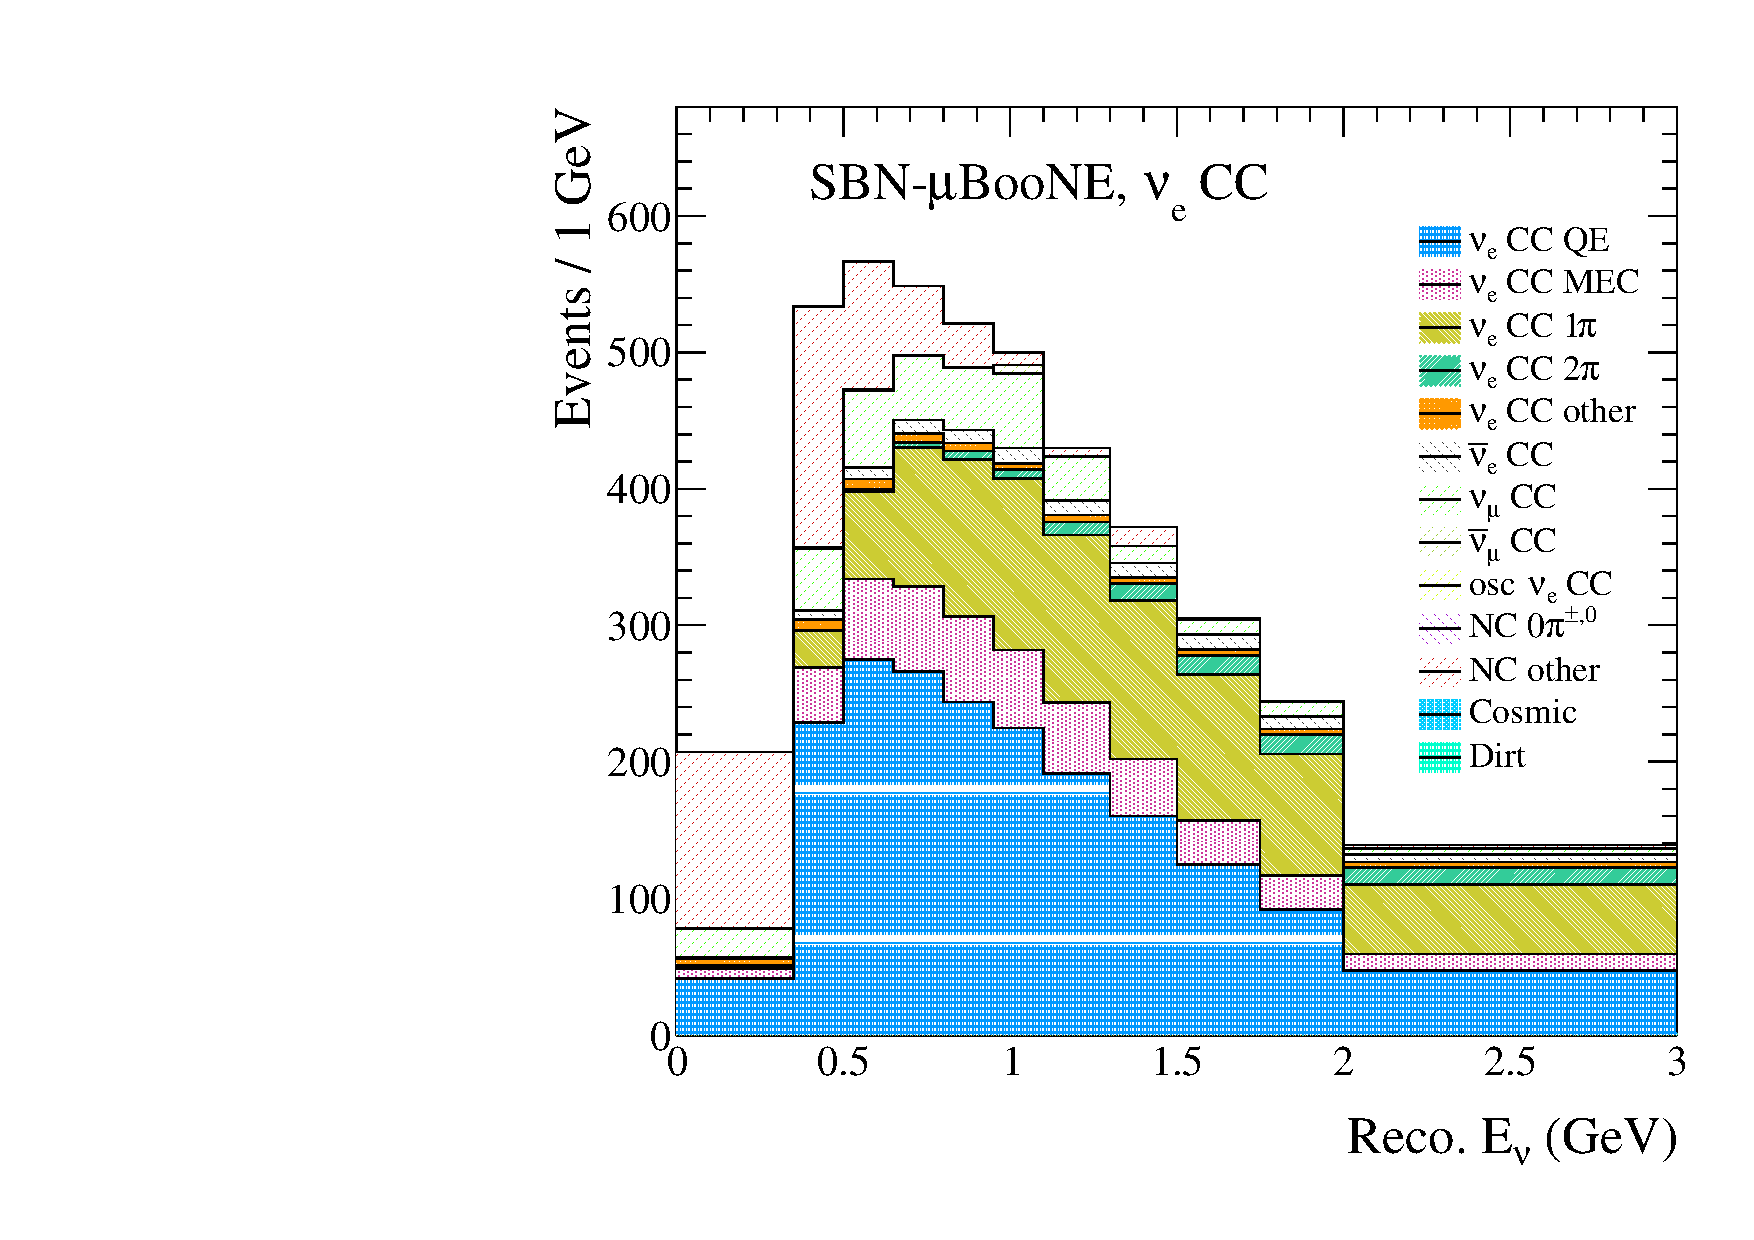
\includegraphics[width=0.49\textwidth]{figures-chap6/spectra/nue_nominal_spectrum_sbn_uboone_BNB_FHC_1_modes.pdf}}
  {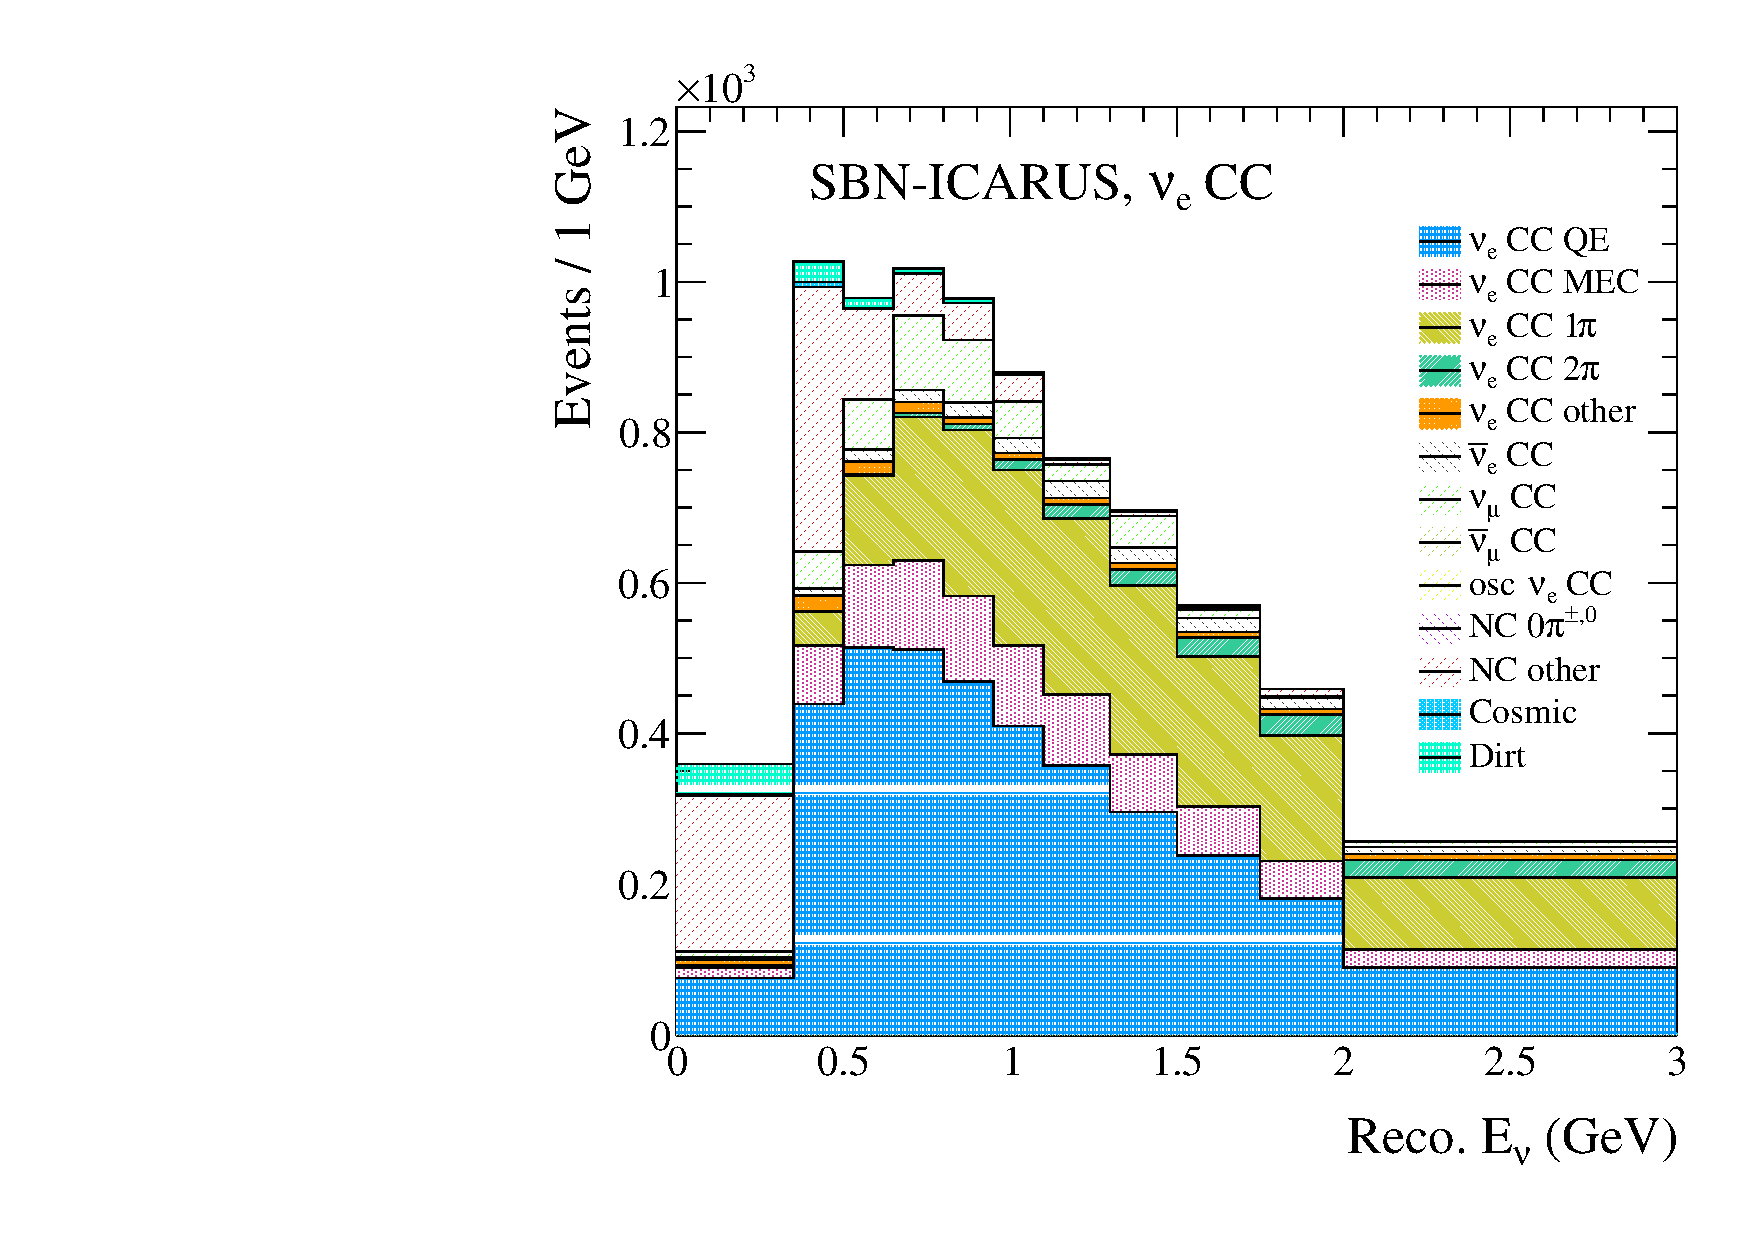
\includegraphics[width=0.49\textwidth]{figures-chap6/spectra/nue_nominal_spectrum_sbn_icarus_BNB_FHC_2_modes.pdf}}
  \captionsetup{width=0.49\textwidth}
  \parbox[b]{0.49\textwidth}%
  {
    \caption[SBN \nue \gls{cc} inclusive reconstructed neutrino energy spectra.]{SBND (top-left), MicroBooNE (top-right) and ICARUS (bottom)
    reconstructed neutrino energy spectra constructed from the samples of $\nue$~\gls{cc}~inclusive events. The spectra are broken down into the
    contributions from each neutrino interaction mode.\\ \phantom{.}\\}
    \label{fig:nominal_nue_spectra} 
  }
\end{figure}

\begin{figure}[h!]
  {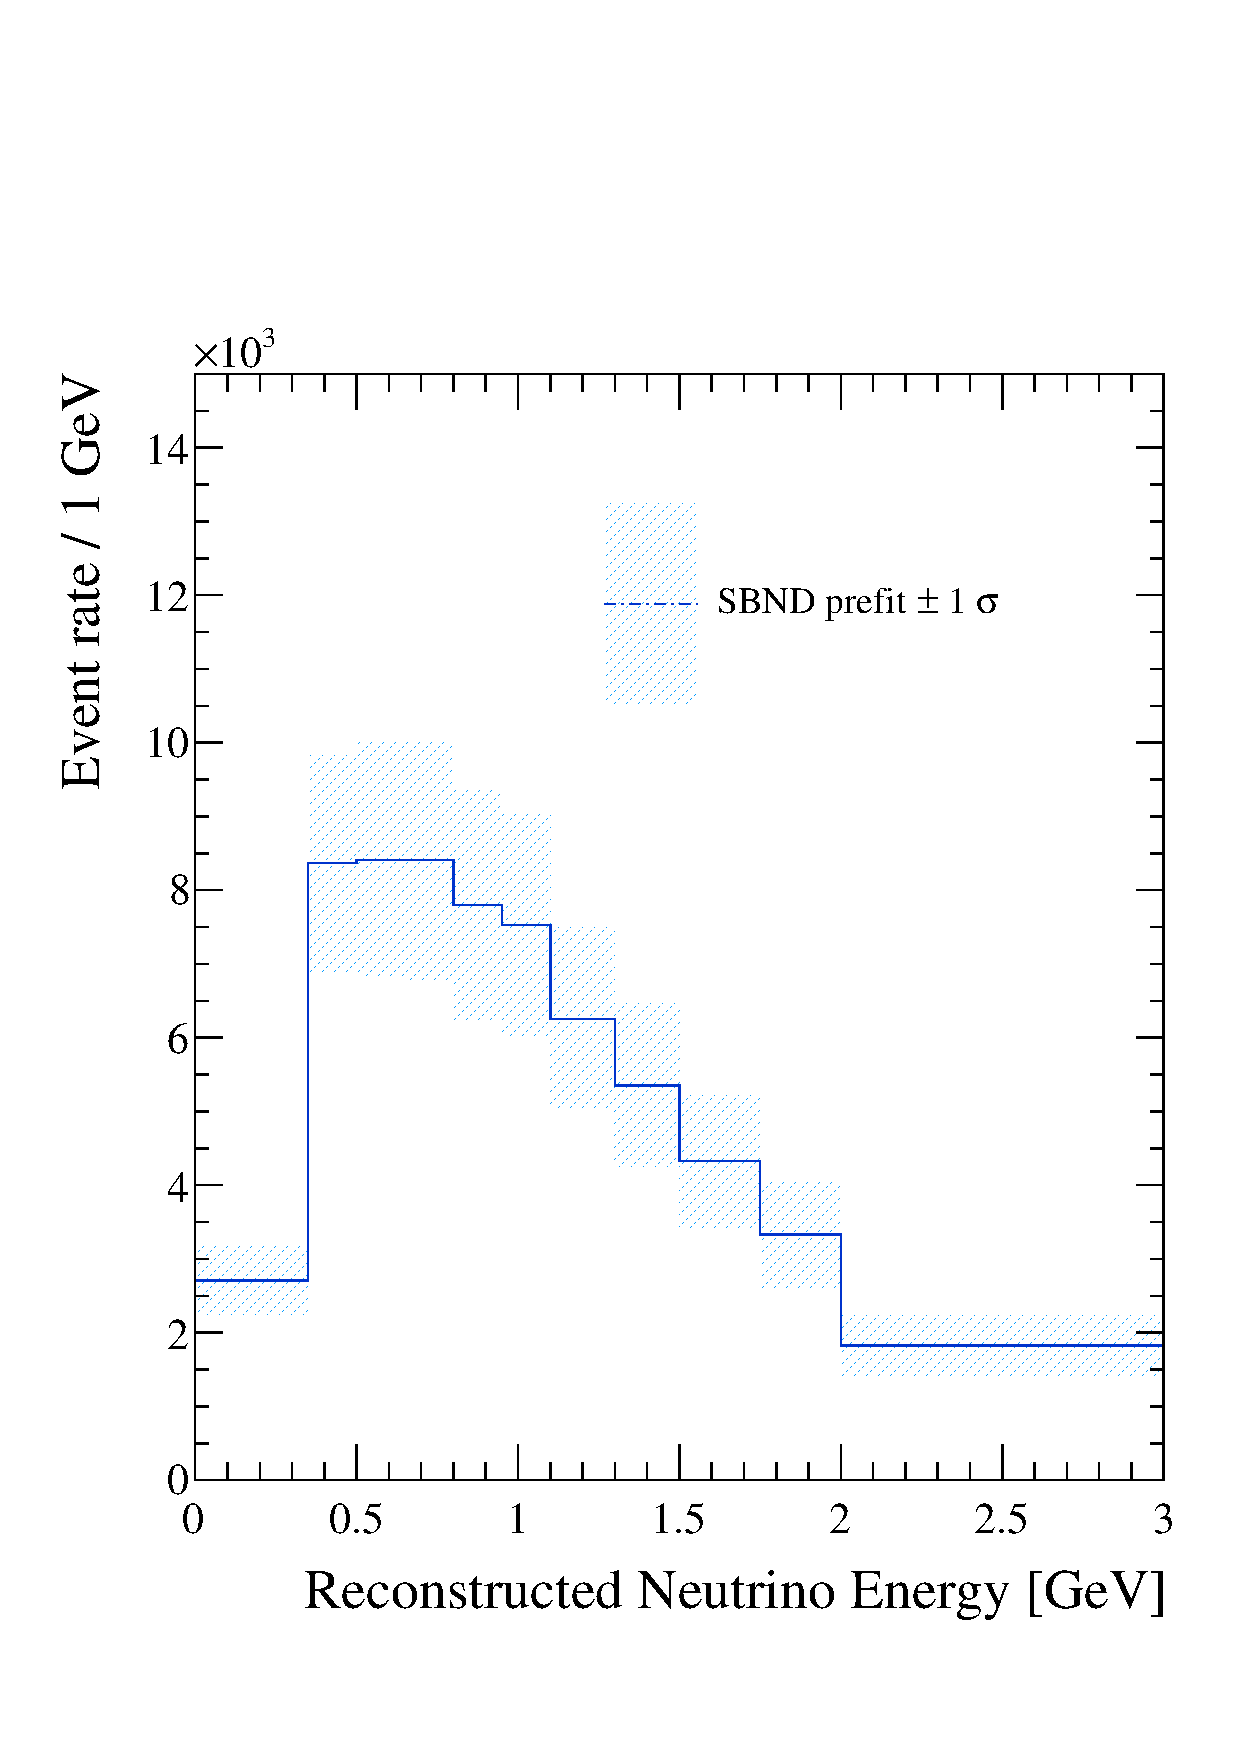
\includegraphics[width=0.49\textwidth]{figures-chap6/spectra/envelopes/sbnd_1sigma_prefit.pdf}}
  {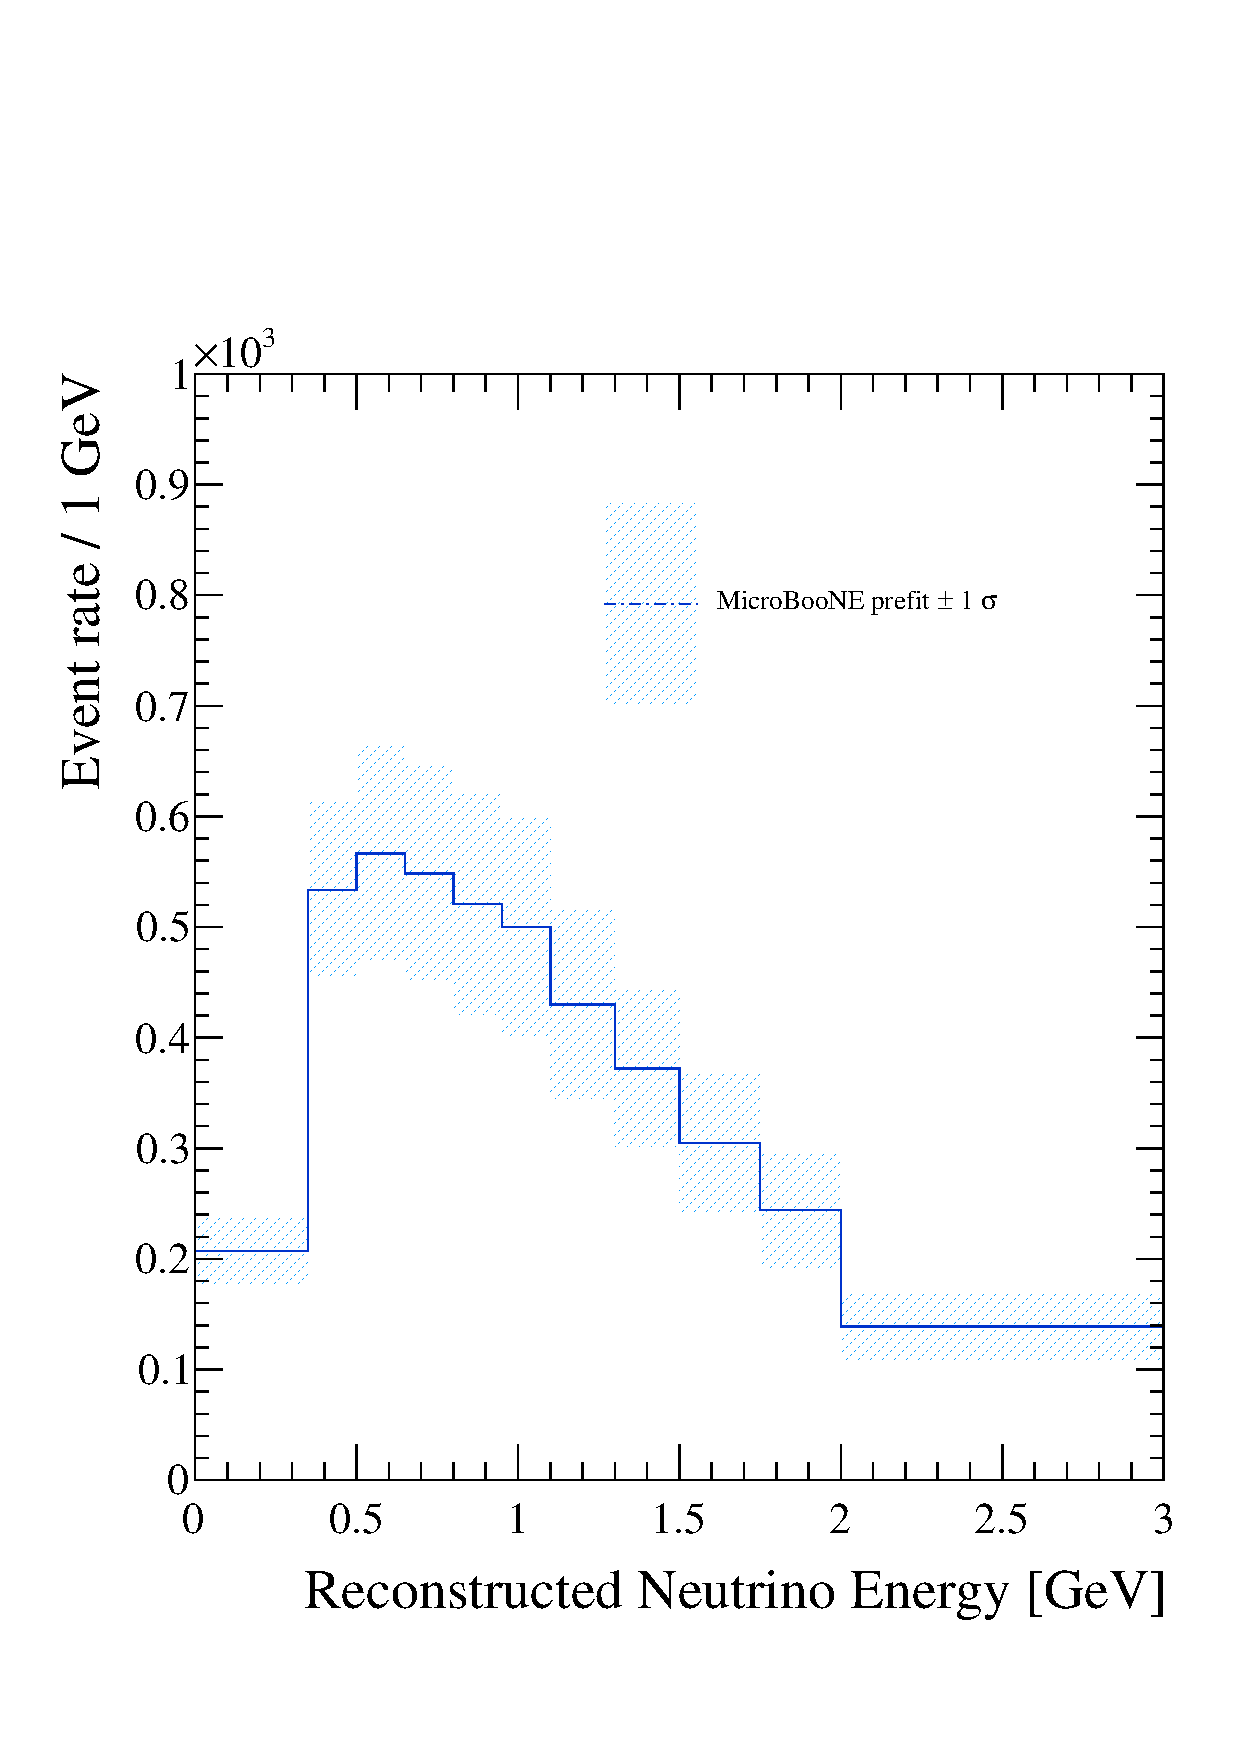
\includegraphics[width=0.49\textwidth]{figures-chap6/spectra/envelopes/uboone_1sigma_prefit.pdf}}
  {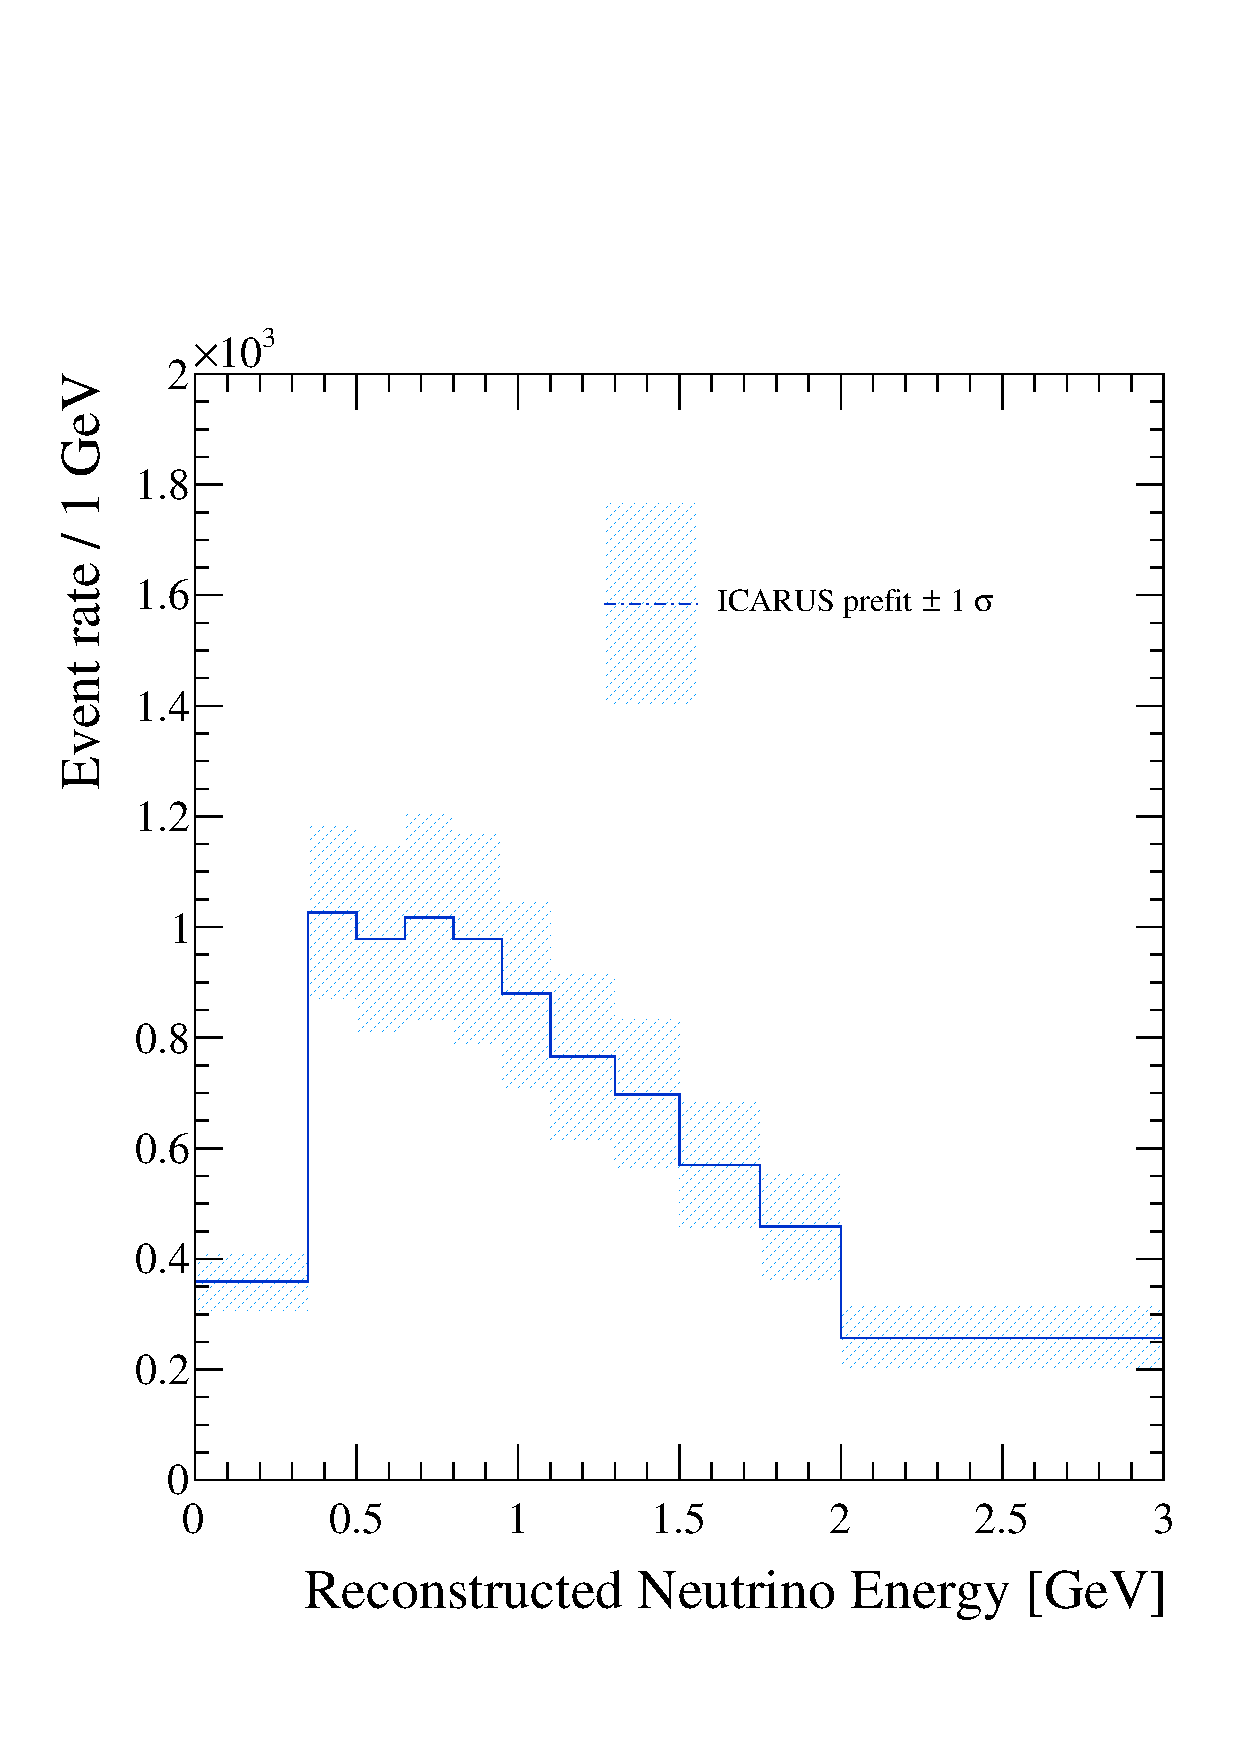
\includegraphics[width=0.49\textwidth]{figures-chap6/spectra/envelopes/icarus_1sigma_prefit.pdf}}
  \captionsetup{width=0.49\textwidth}
  \parbox[b]{0.49\textwidth}%
  {
    \caption[SBN \nue \gls{cc} inclusive reconstructed neutrino energy spectra with a 1$\sigma$ prefit envelopes.]{SBND (top-left), MicroBooNE (top-right) and ICARUS (bottom) integrated reconstructed neutrino energy spectra constructed from the samples of $\nue$~\gls{cc}~inclusive events. A 1$\sigma$ prefit uncertainty envelope from the flux and interaction systematics is also shown. \\\phantom{.}\\\phantom{.}\\\phantom{.}\\}
    \label{fig:nominal_nue_spectra_1sigma_enevelope} 
  }
\end{figure}

\begin{figure}[h!]
    \centering
    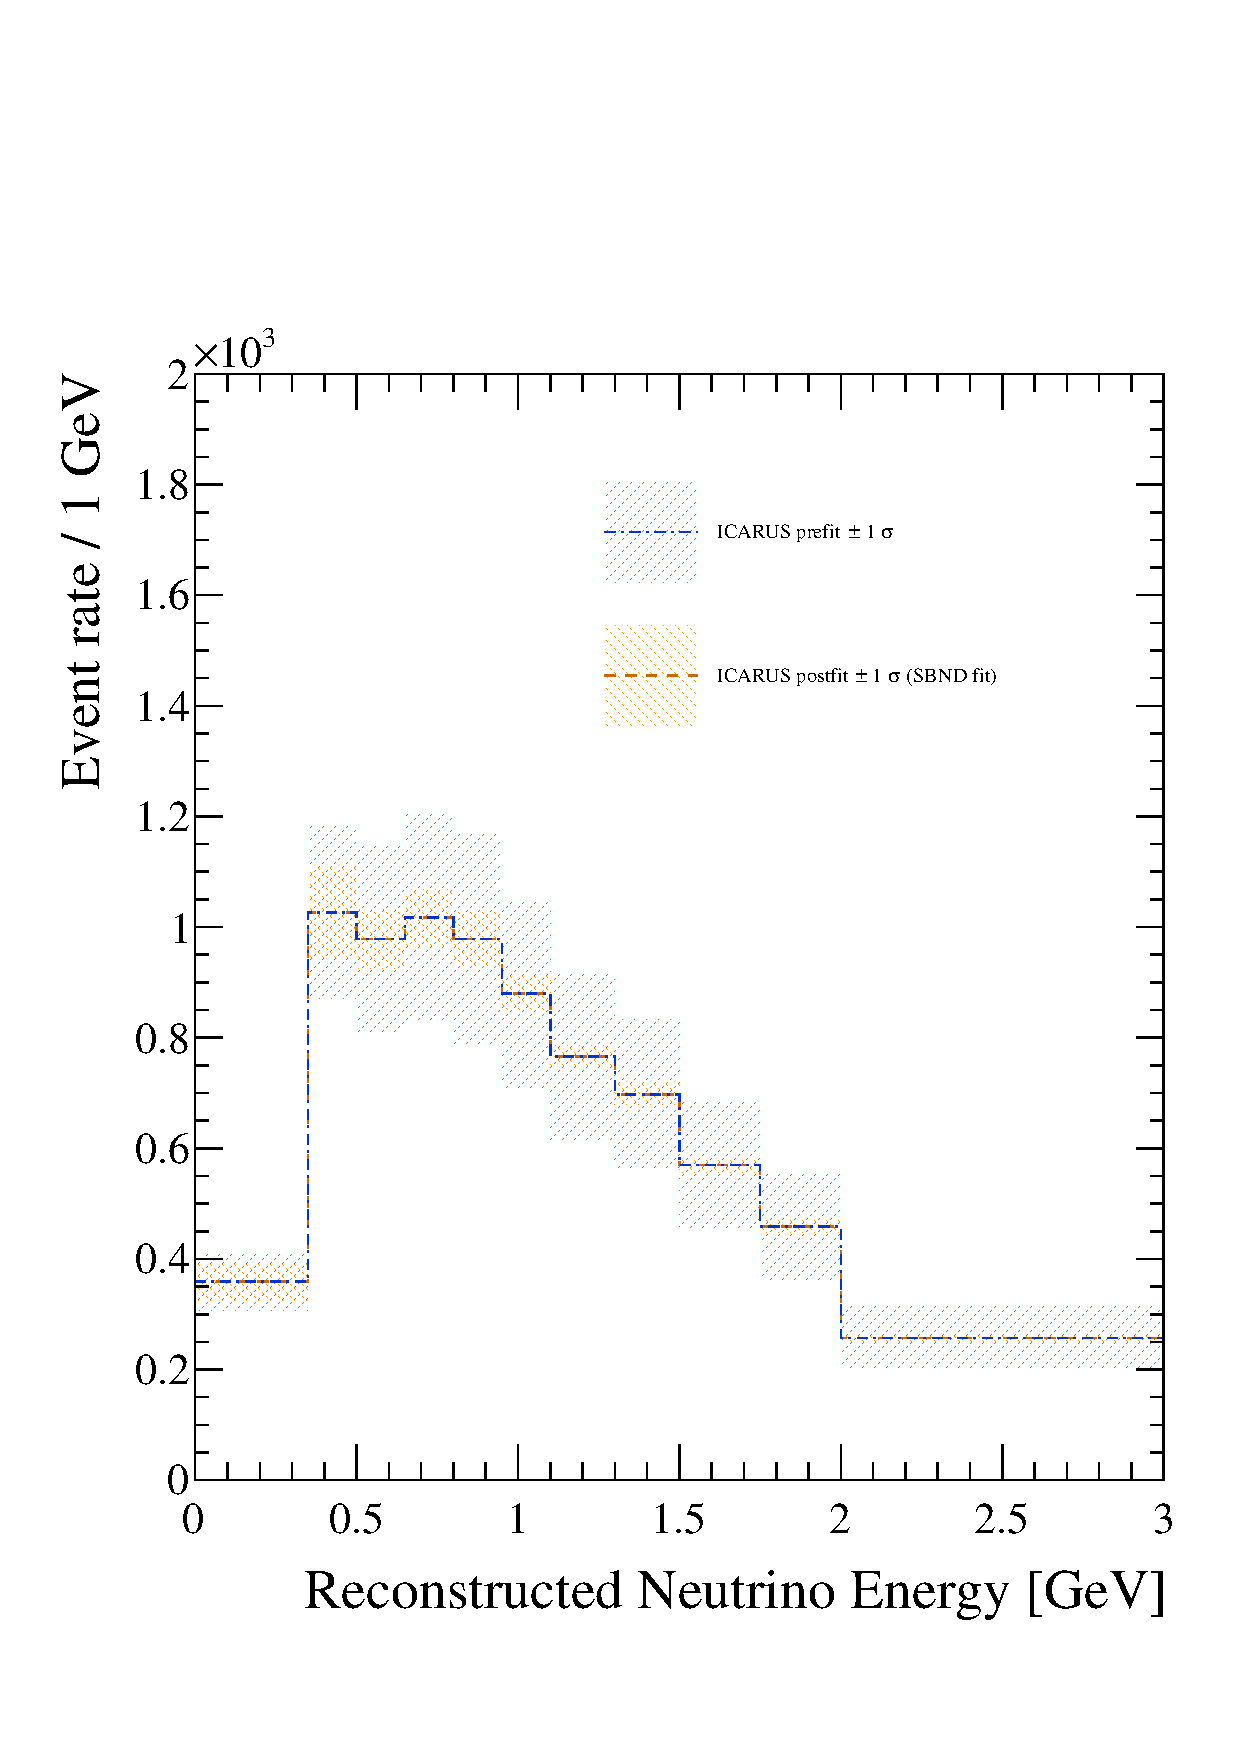
\includegraphics[width = \largefigwidth]{figures-chap6/spectra/envelopes/icarus_pre_post_fit_nue.pdf}
    \caption[ICARUS \nue \gls{cc} inclusive neutrino energy spectra with a 1$\sigma$ prefit and postfit envelope.]{ICARUS integrated reconstructed neutrino energy spectrum constructed from the samples of \nue~\gls{cc}~inclusive events. The $1\sigma$ prefit envelope is shown as well as a $1\sigma$ postfit envelope based on an \gls{sbnd} fit. The reduction in size of the error envelope when going from prefit to postfit shows the impact of \gls{sbnd} on improving the accuracy of the ICARUS prediction.}
    \label{fig:icarus_pre_post_fit}
\end{figure}


\clearpage
\subsection{Expected Oscillation Signal}

Assuming that mixing with a light sterile neutrino occurs, a change to the nominal event rate will be observed. Since the oscillation channels are currently considered as stand-alone analyses, this will either result in an increase or decrease in the event rate depending on whether an appearance or disappearance channel is considered. 

\subsubsection{\texorpdfstring{\nue Appearance Analysis}{nue Appearance Analysis}}\label{sec:nue_app}

The \nue appearance channel is concerned with oscillations from \numu to \nue meaning an increase in the event rate is expected. This is shown in \FigureRef{fig:nue_spectra_with_osc_overlay} where the nominal event rate breakdown is shown as in \FigureRef{fig:nominal_nue_spectra} but overlaid with an integrated spectrum that was produced with oscillation parameters \mbox{$\sin^2{2\theta_{\mu e}} = 0.003$} and $\Delta m^2_{41} = 1.32 \text{ eV}^2$. The oscillation signal seen for these parameters in \gls{sbnd} is small whereas for \gls{microboone} and \gls{icarus} it is substantial which is consistent with what is seen in \FigureRef{fig:osc_probability}. This highlights the fact that \gls{sbnd} will largely be used to constrain systematic parameters due to observing no or very few oscillated events with the oscillation signal being largely left to \gls{microboone} and \gls{icarus}. 


\begin{figure}[h!]
  {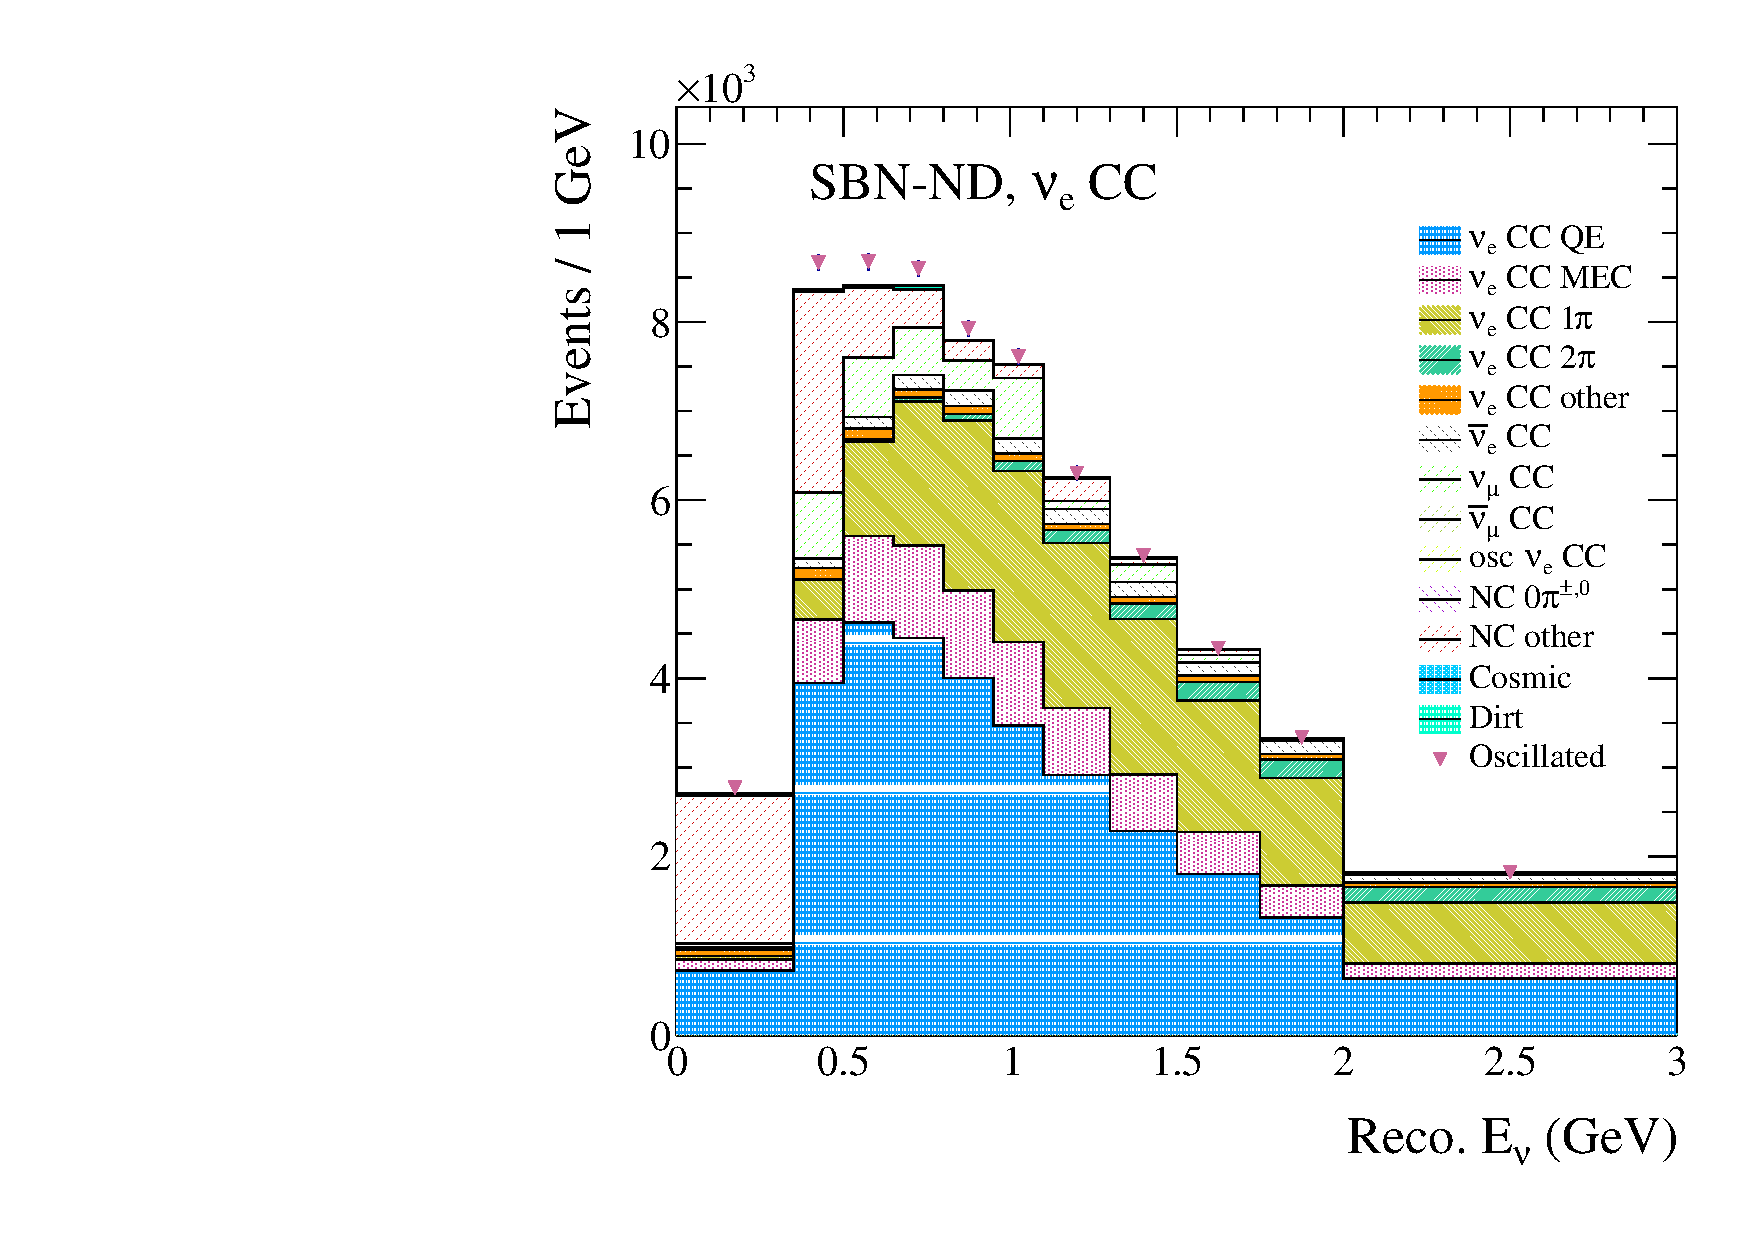
\includegraphics[width=0.49\textwidth]{figures-chap6/spectra/nue_app_dmsq_1.32_sinsq_0.003_overlay_spectrum_sbn_nd_BNB_FHC_0_modes.pdf}}
  {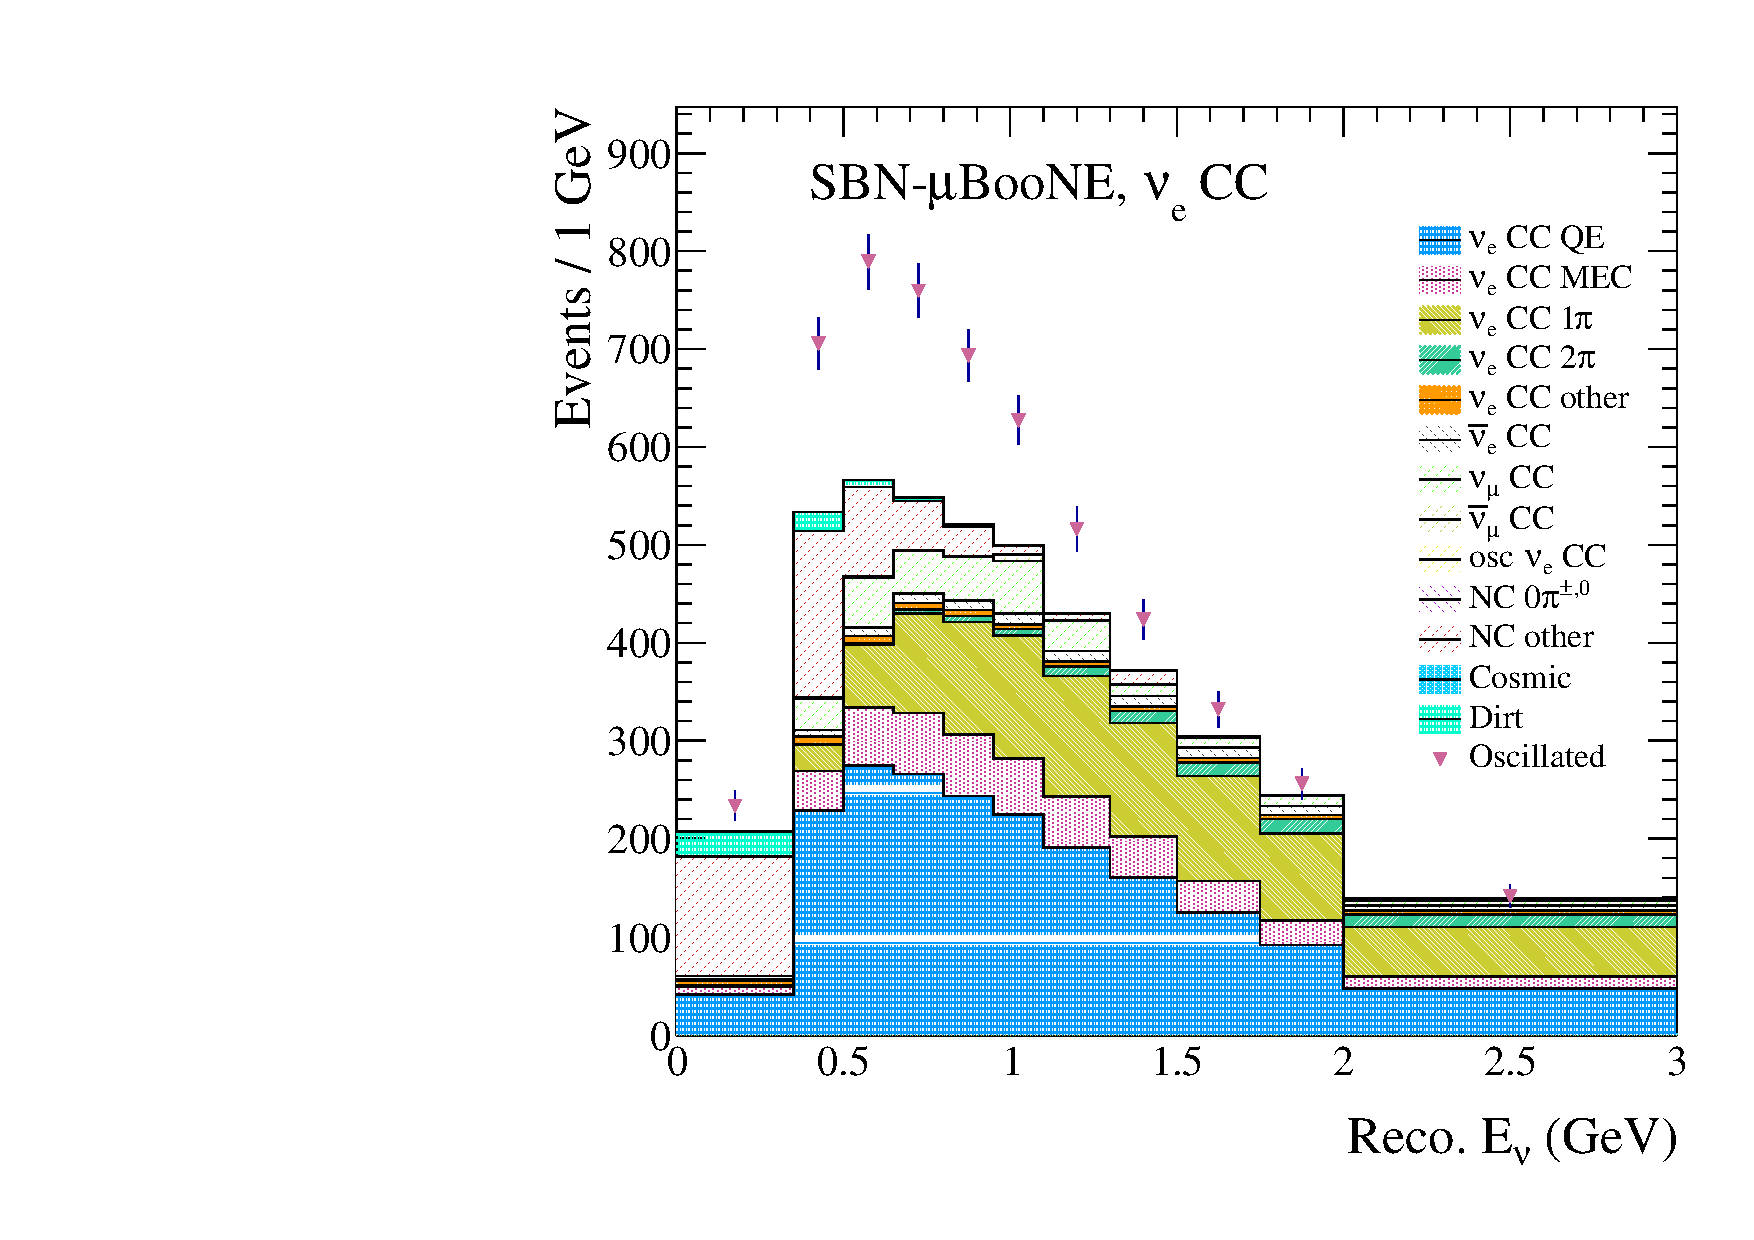
\includegraphics[width=0.49\textwidth]{figures-chap6/spectra/nue_app_dmsq_1.32_sinsq_0.003_overlay_spectrum_sbn_uboone_BNB_FHC_1_modes.pdf}}
  {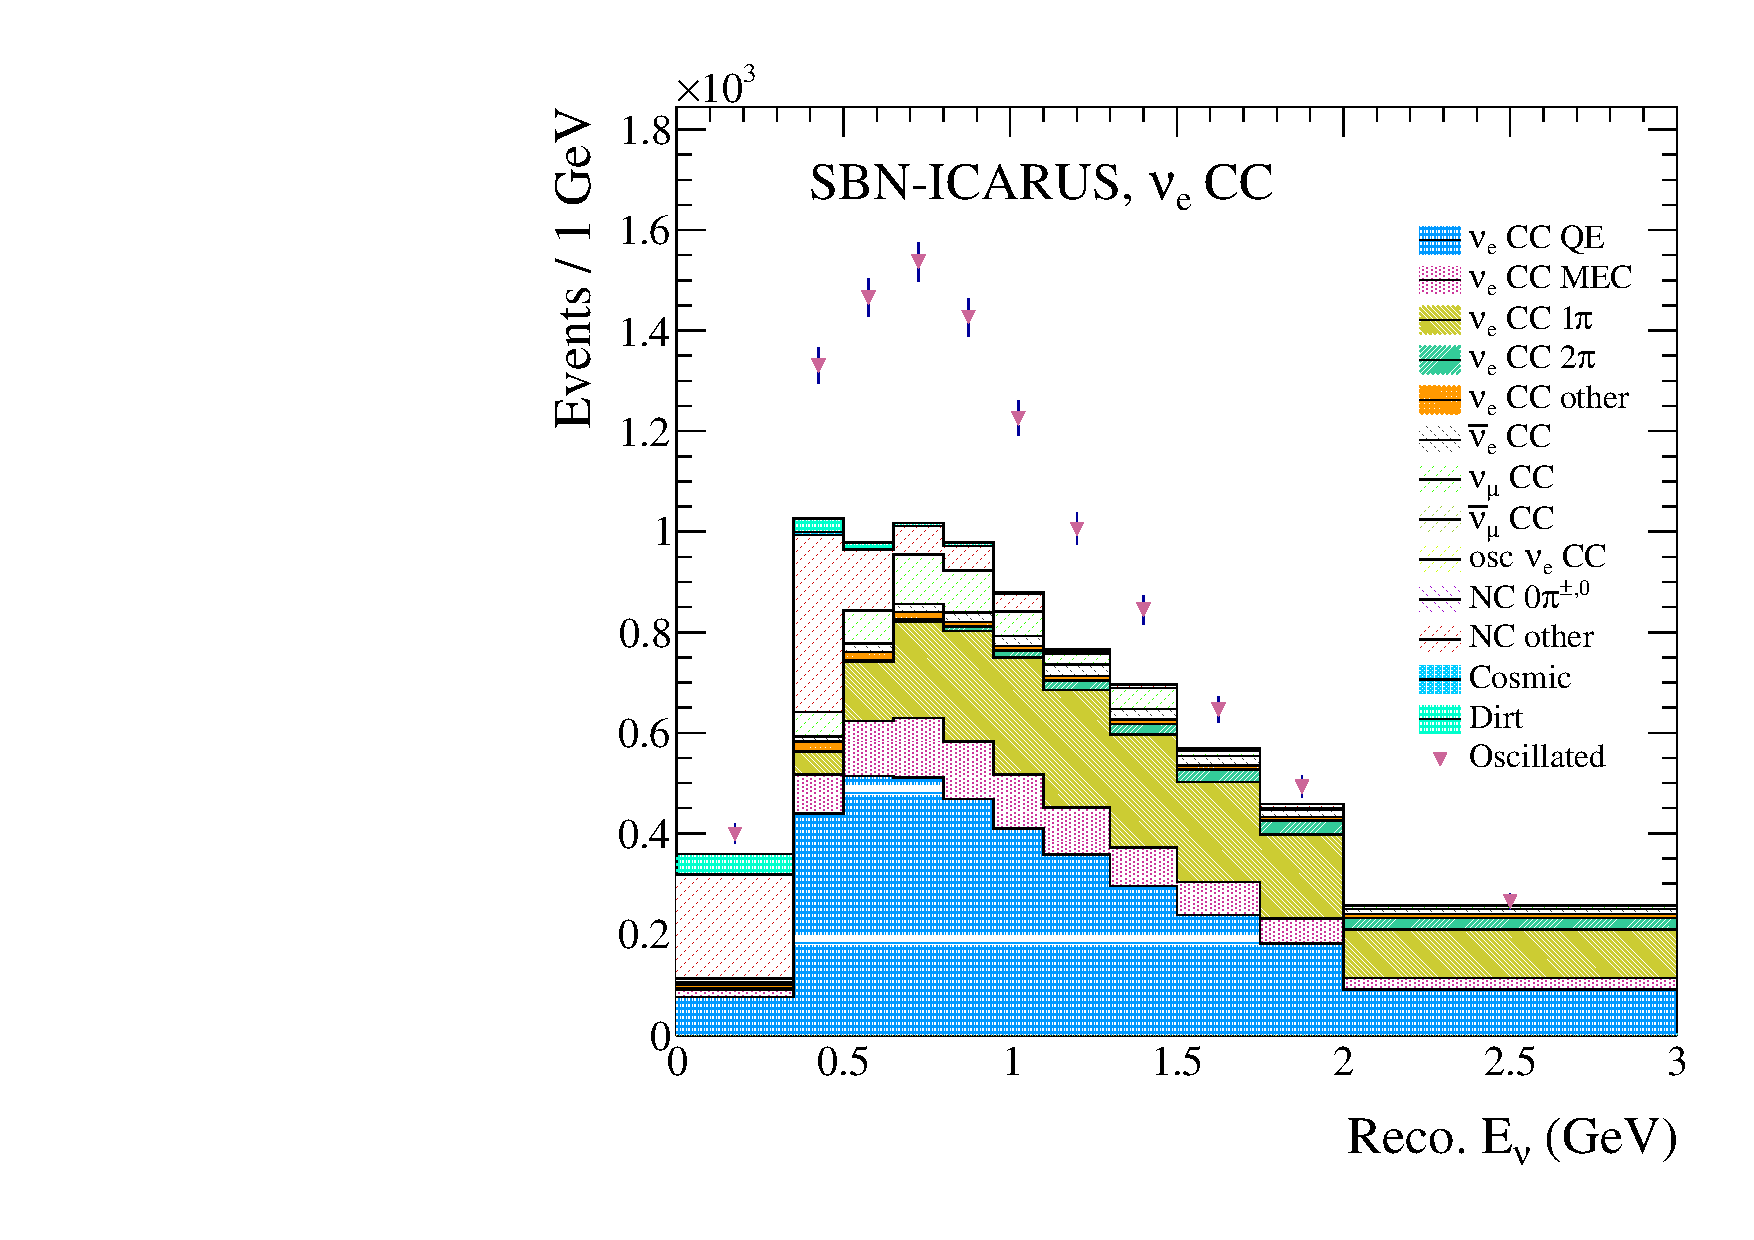
\includegraphics[width=0.49\textwidth]{figures-chap6/spectra/nue_app_dmsq_1.32_sinsq_0.003_overlay_spectrum_sbn_icarus_BNB_FHC_2_modes.pdf}}
  \captionsetup{width=0.49\textwidth}
  \parbox[b]{0.49\textwidth}%
  {
    \caption[SBN \nue appearance \gls{cc} inclusive reconstructed neutrino energy spectra with oscillated spectrum overlaid.]{The nominal spectra as in \FigureRef{fig:nominal_nue_spectra} but an additional integrated oscillated spectrum with oscillation parameters, $\sin^2{2\theta_{\mu e}} = 0.003$ and $\Delta m^2_{41} = 1.32$ eV$^2$ has been overlaid showing the increase in event rate. \\\phantom{.}\\\phantom{.}\\\phantom{.}\\
    \label{fig:nue_spectra_with_osc_overlay}}
    }
\end{figure}

\newpage
The top left plot of Figure~\ref{fig:Nue_app_spectra_ratios} shows the \nue appearance statistical only exclusion contour and allowed region from fits combining all three \gls{sbn} detectors. The injected point $\Delta m^2_{41} = 1.32$ eV$^2$, $\sin^2{2\theta_{\mu e}} = 0.003$, used when producing the allowed region is shown along with two further points on the exclusion contour at $\Delta m^2_{41} = 1$ eV$^2$, $\sin^2{2\theta_{\mu e}} = 0.0014$ and $\Delta m^2_{41} = 100$ eV$^2$, $\sin^2{2\theta_{\mu e}} = 0.0005$. \nue appearance spectra are produced using oscillation parameters corresponding to each of these three points for each of the three SBN detectors. The ratio of each of these oscillated spectra to the nominal for each detector are shown in the remaining plots in Figure~\ref{fig:Nue_app_spectra_ratios} and highlight the expected oscillation signal.


\begin{figure}[h!]
    \centering
    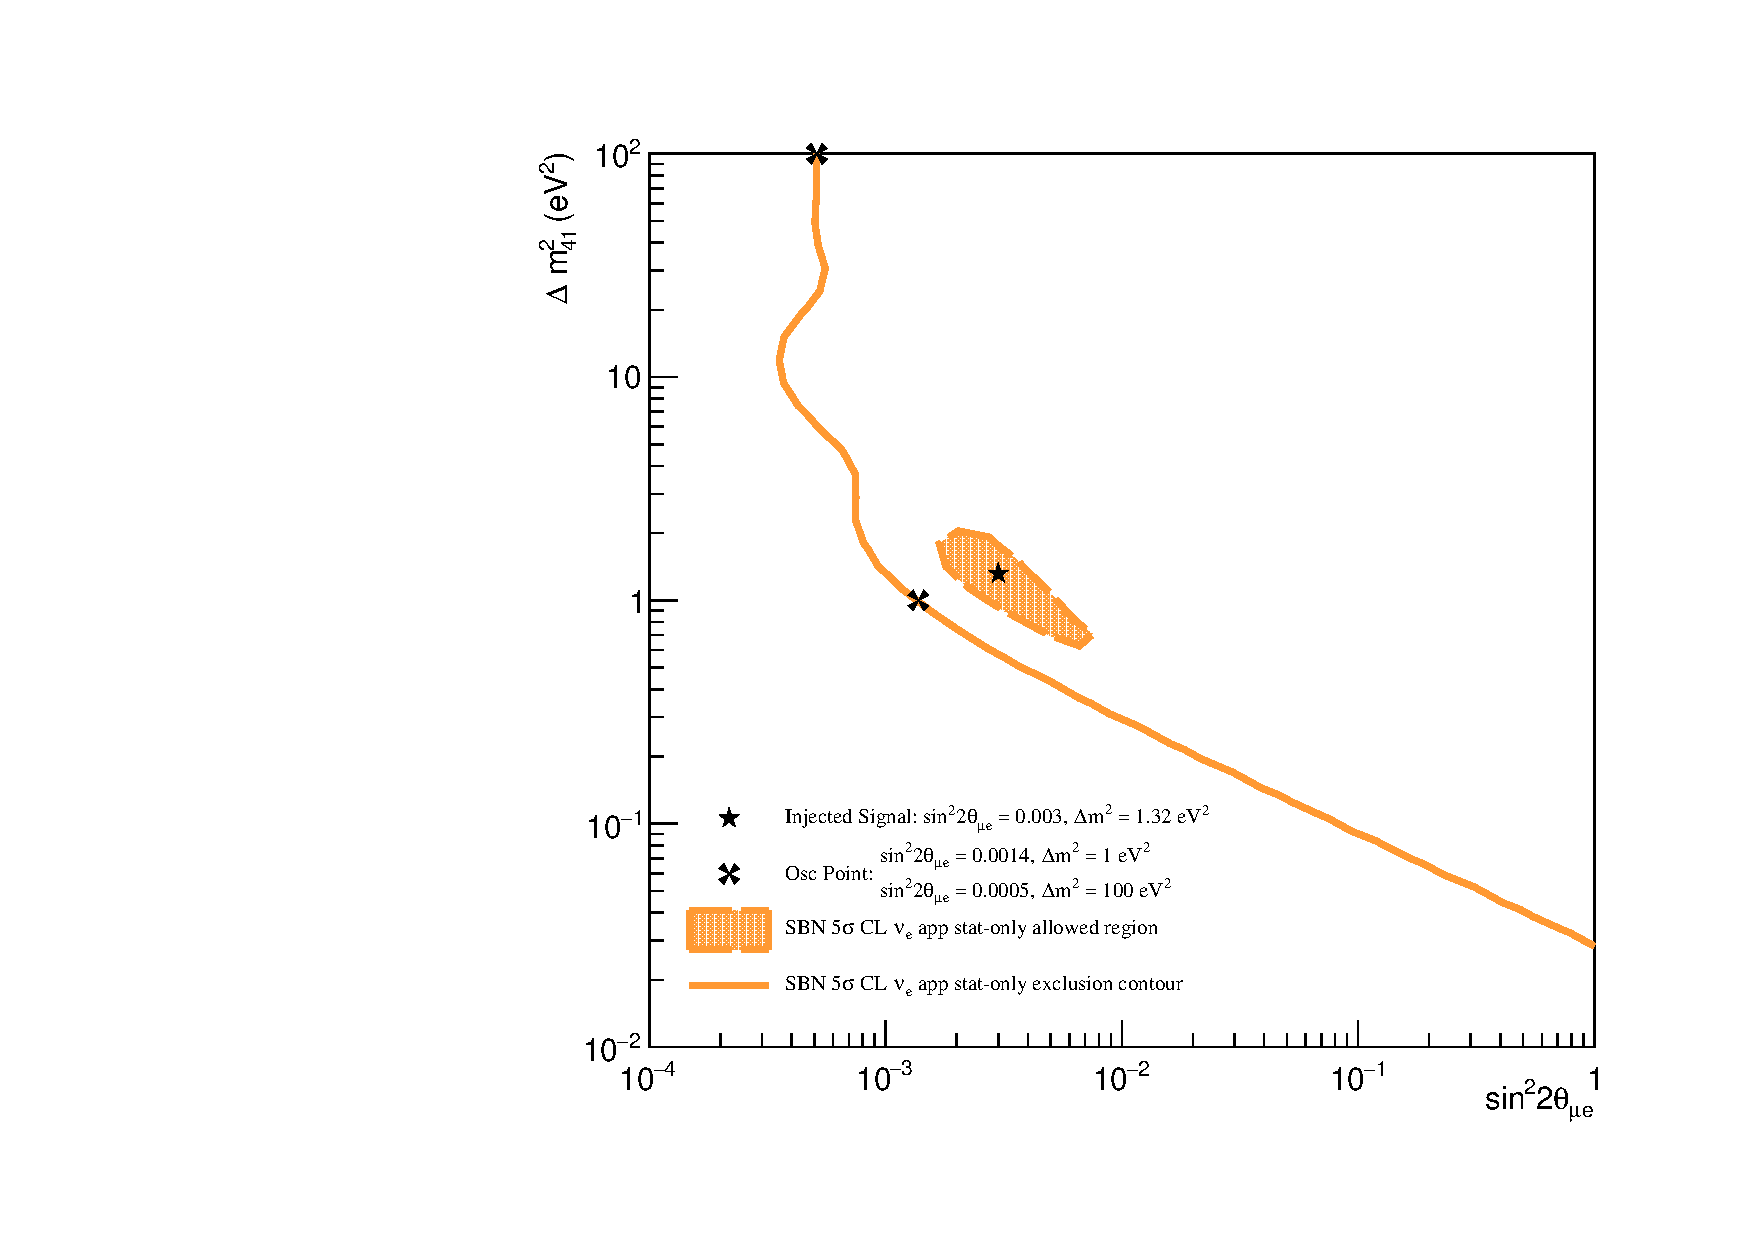
\includegraphics[width = 0.49\textwidth, height = 0.47\textwidth]{figures-chap6/overlays/nue_app_stat_osc_markers.pdf}
    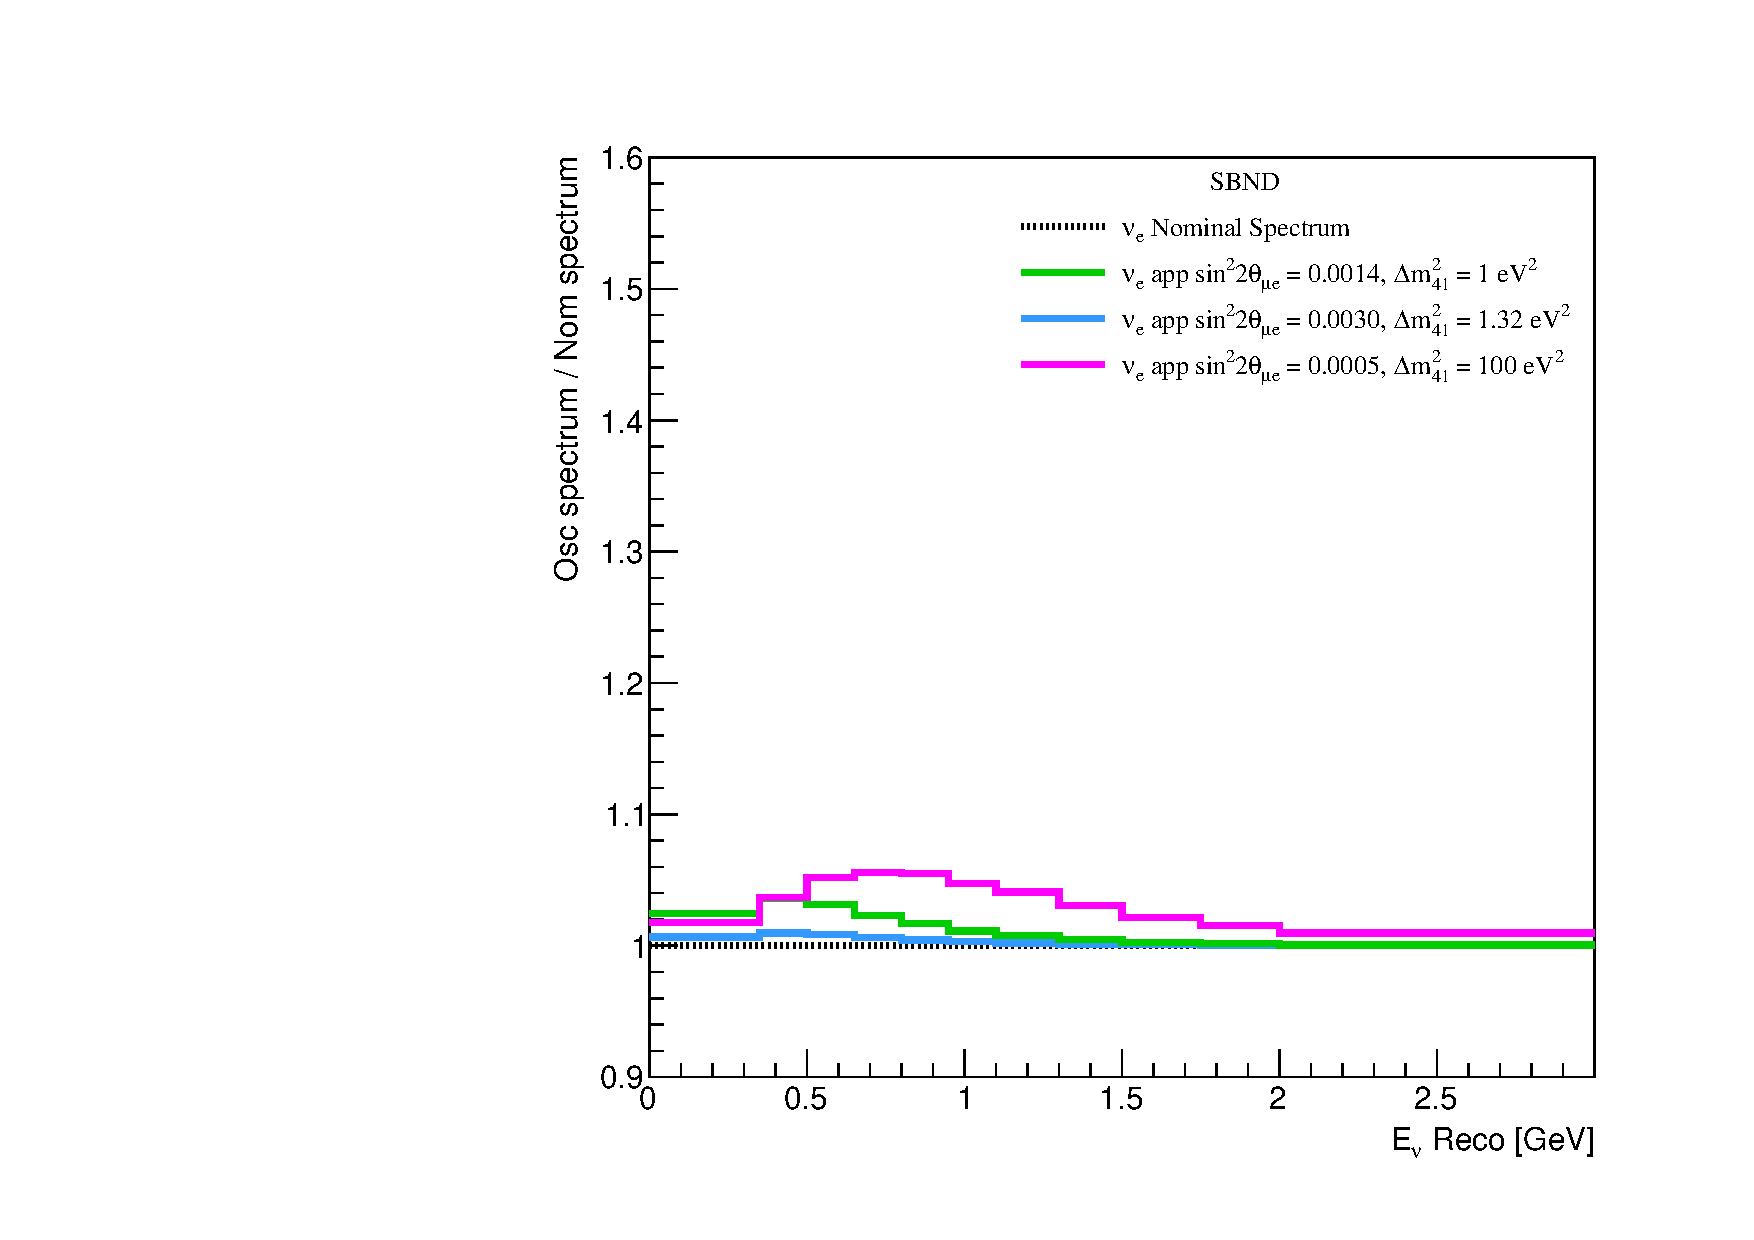
\includegraphics[width = 0.49\textwidth]{figures-chap6/spectra/nue_app_spectra_ratio_sbnd.pdf}
    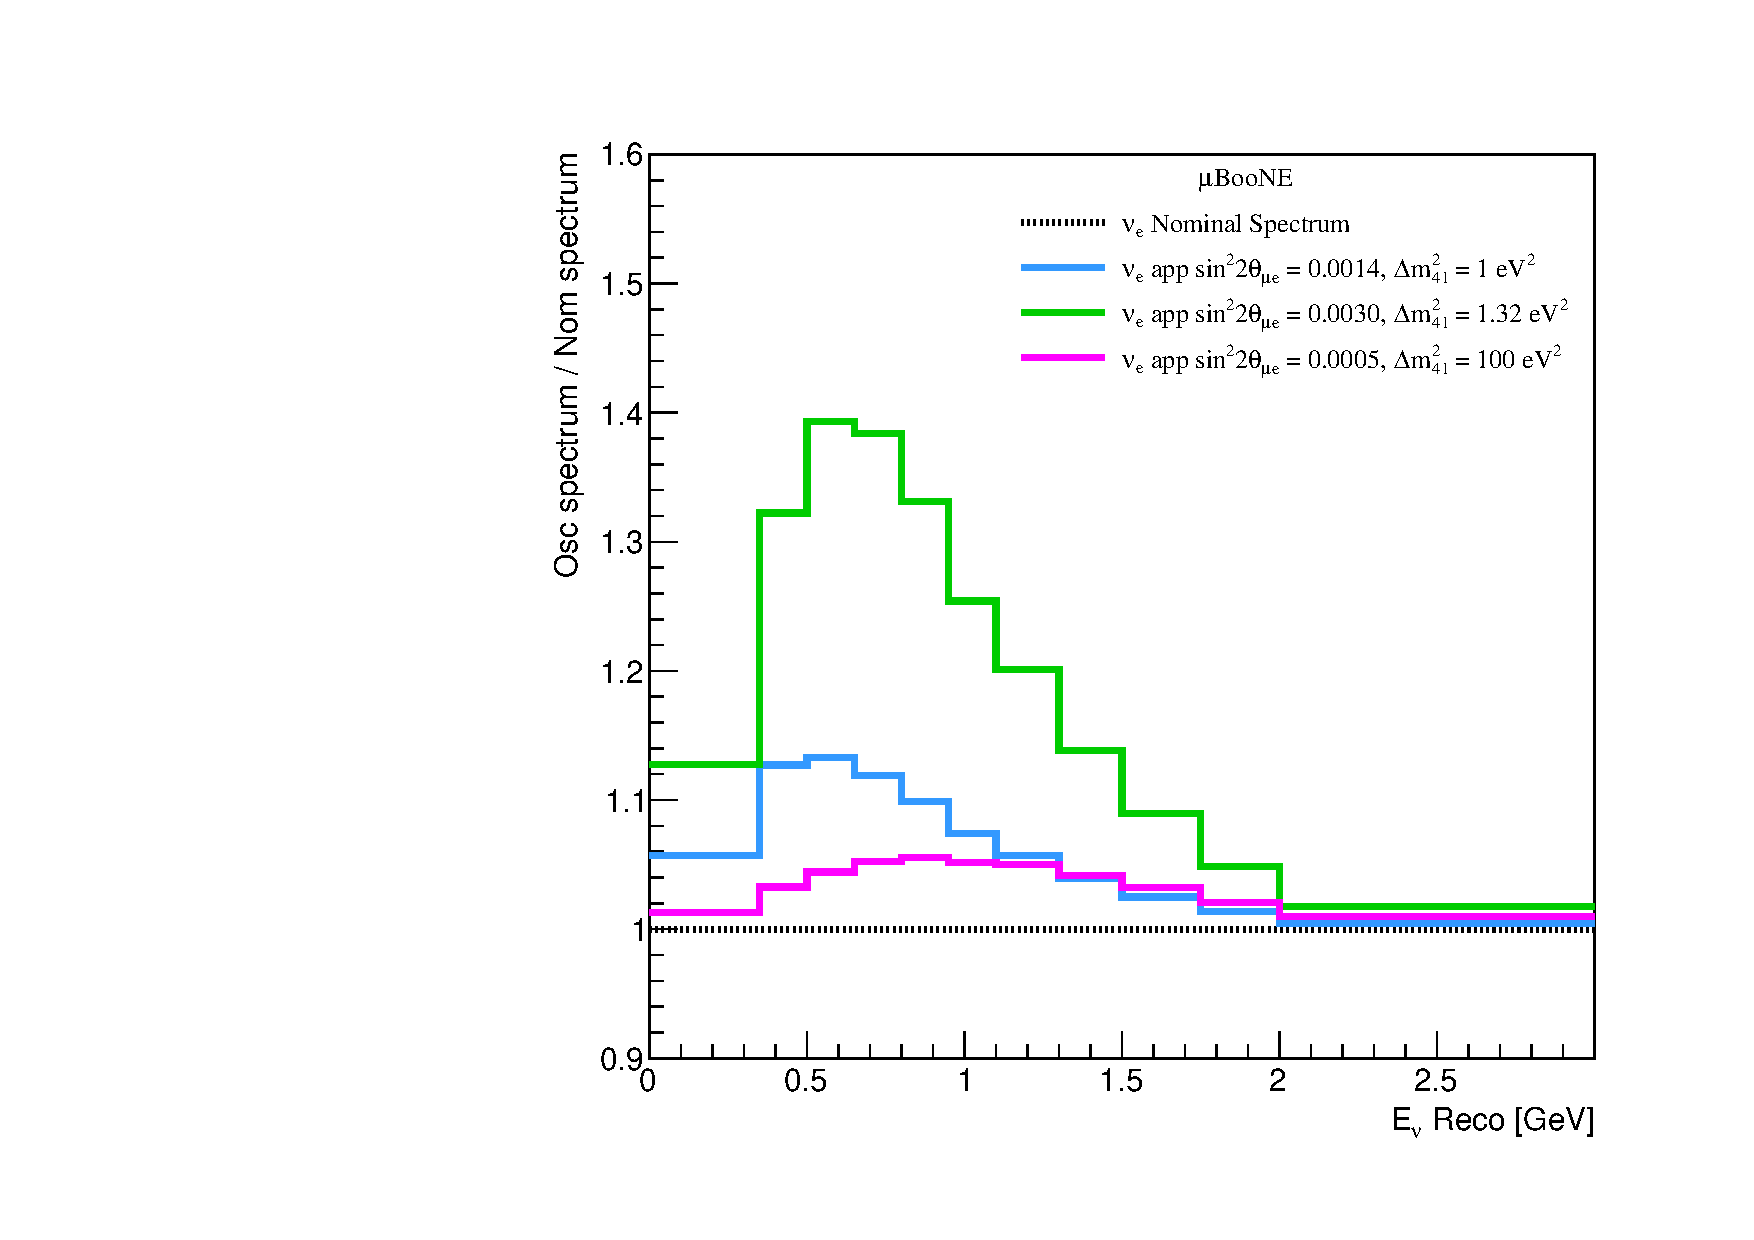
\includegraphics[width = 0.49\textwidth]{figures-chap6/spectra/nue_app_spectra_ratio_uboone.pdf}
    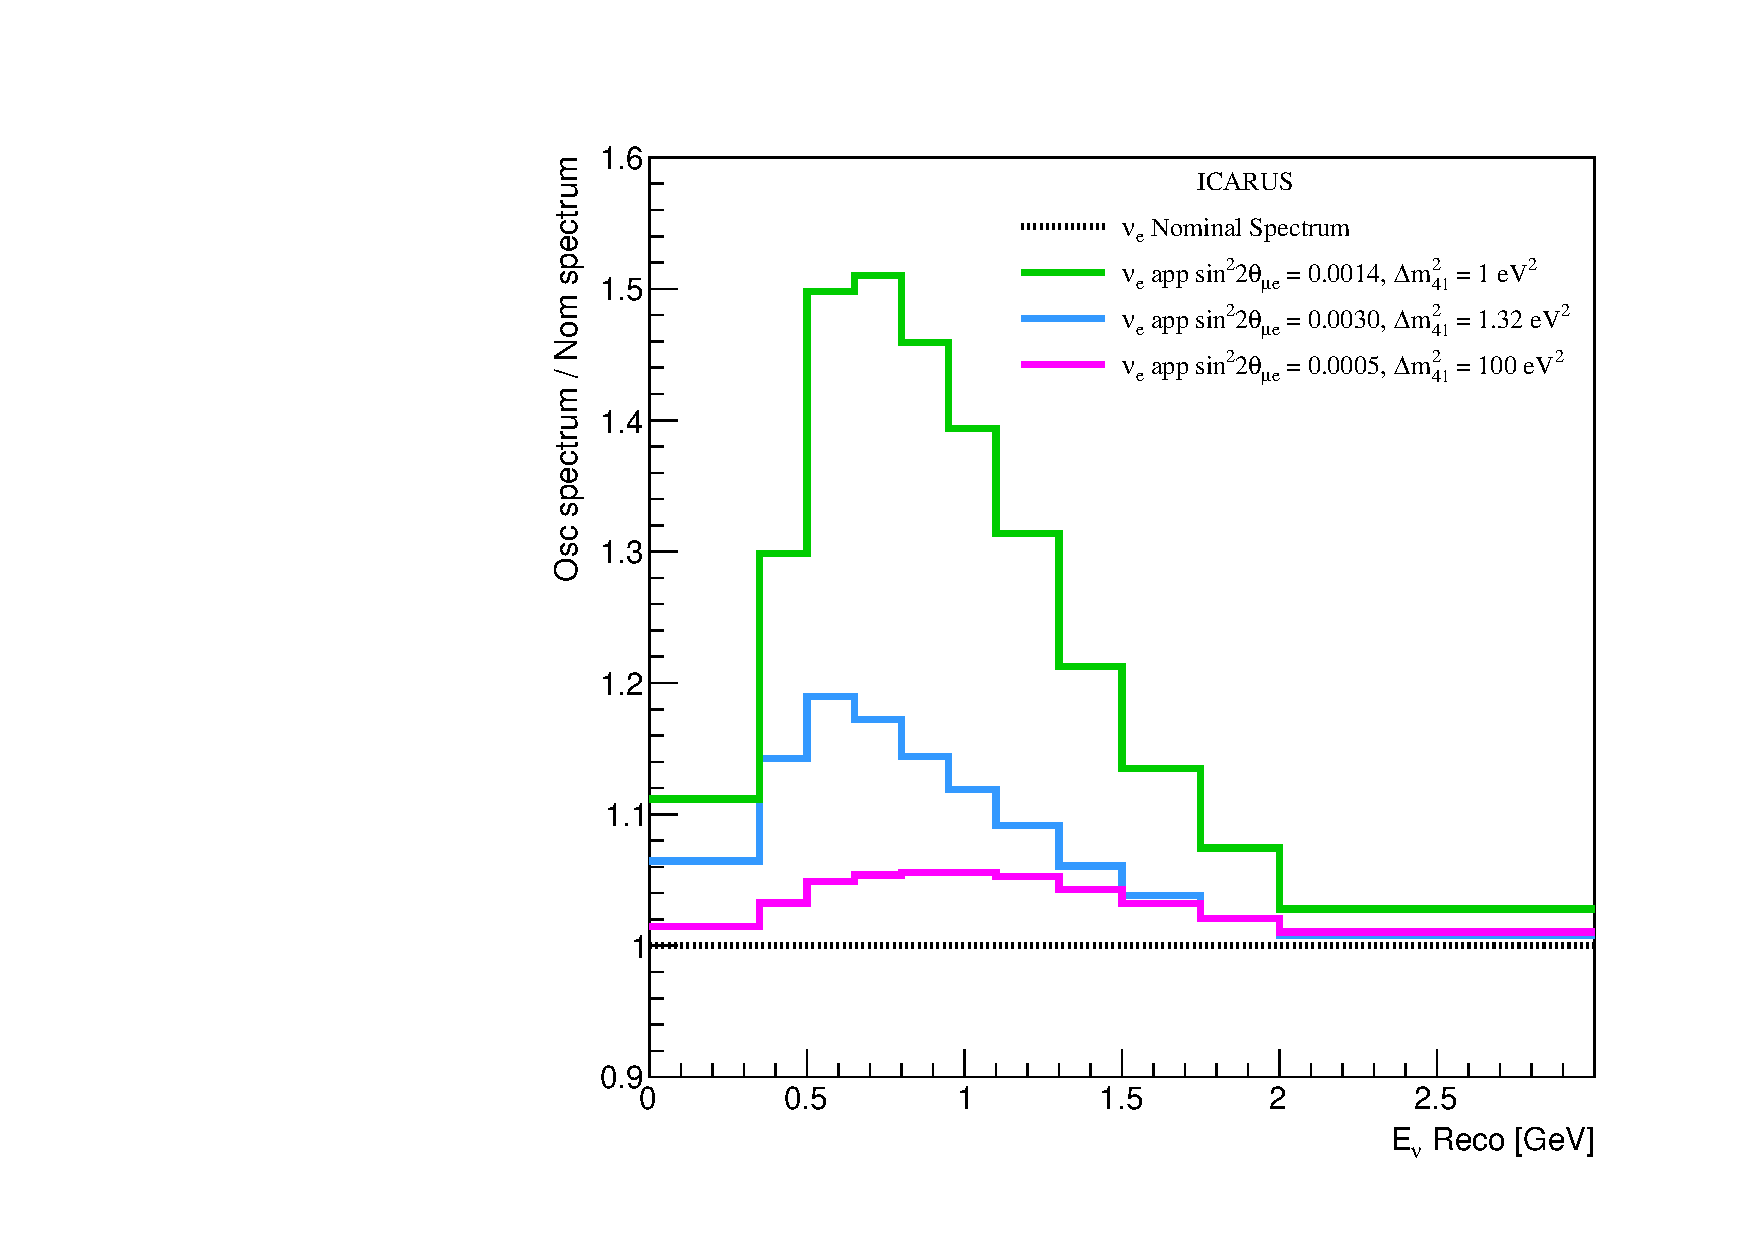
\includegraphics[width = 0.49\textwidth]{figures-chap6/spectra/nue_app_spectra_ratio_icarus.pdf}
    \caption[Ratio of \nue appearance spectra with the oscillation parameters shown on the statistical only contour.]{\nue appearance stat-only exclusion contour and allowed region. The injected point at $\sin^2{2\theta_{\mu e}} = 0.003$, $\Delta m^2_{41}$ = 1.32 eV$^2$ used for the allowed region is shown along with two further points at $\sin^2{2\theta_{\mu e}} = 0.0014$, $\Delta m^2_{41}$ = 1 eV$^2$ and   $\sin^2{2\theta_{\mu e}} = 0.0005$, $\Delta m^2_{41}$ = 100 eV$^2$ (top left). The ratio of spectra with oscillation parameters corresponding to the three points mentioned versus nominal are shown for \gls{sbnd} (top right), \gls{microboone} (bottom left) and \gls{icarus} (bottom right).}
    \label{fig:Nue_app_spectra_ratios}
\end{figure}


\subsubsection{\texorpdfstring{\nue Disappearance Analysis}{nue Disappearance Analysis}}

Mirroring the \nue appearance channel, the \nue disappearance channel observes a reduction in the nominal \nue event rate. This is shown in \FigureRef{fig:nue_disapp_spectra} where the integrated spectrum produced with oscillation parameters $\sin^2{2\theta_{ee}} = 0.4$ and $\Delta m^2_{41} = 3 \text{ eV}^2$ has been overlaid onto the breakdown of the nominal spectrum for each of the three detectors. As is the case for \nue appearance, the oscillation signal is relatively small in \gls{sbnd} whereas both \gls{microboone} and \gls{icarus} observe a much more significant signal. 

\begin{figure}[h!]
  {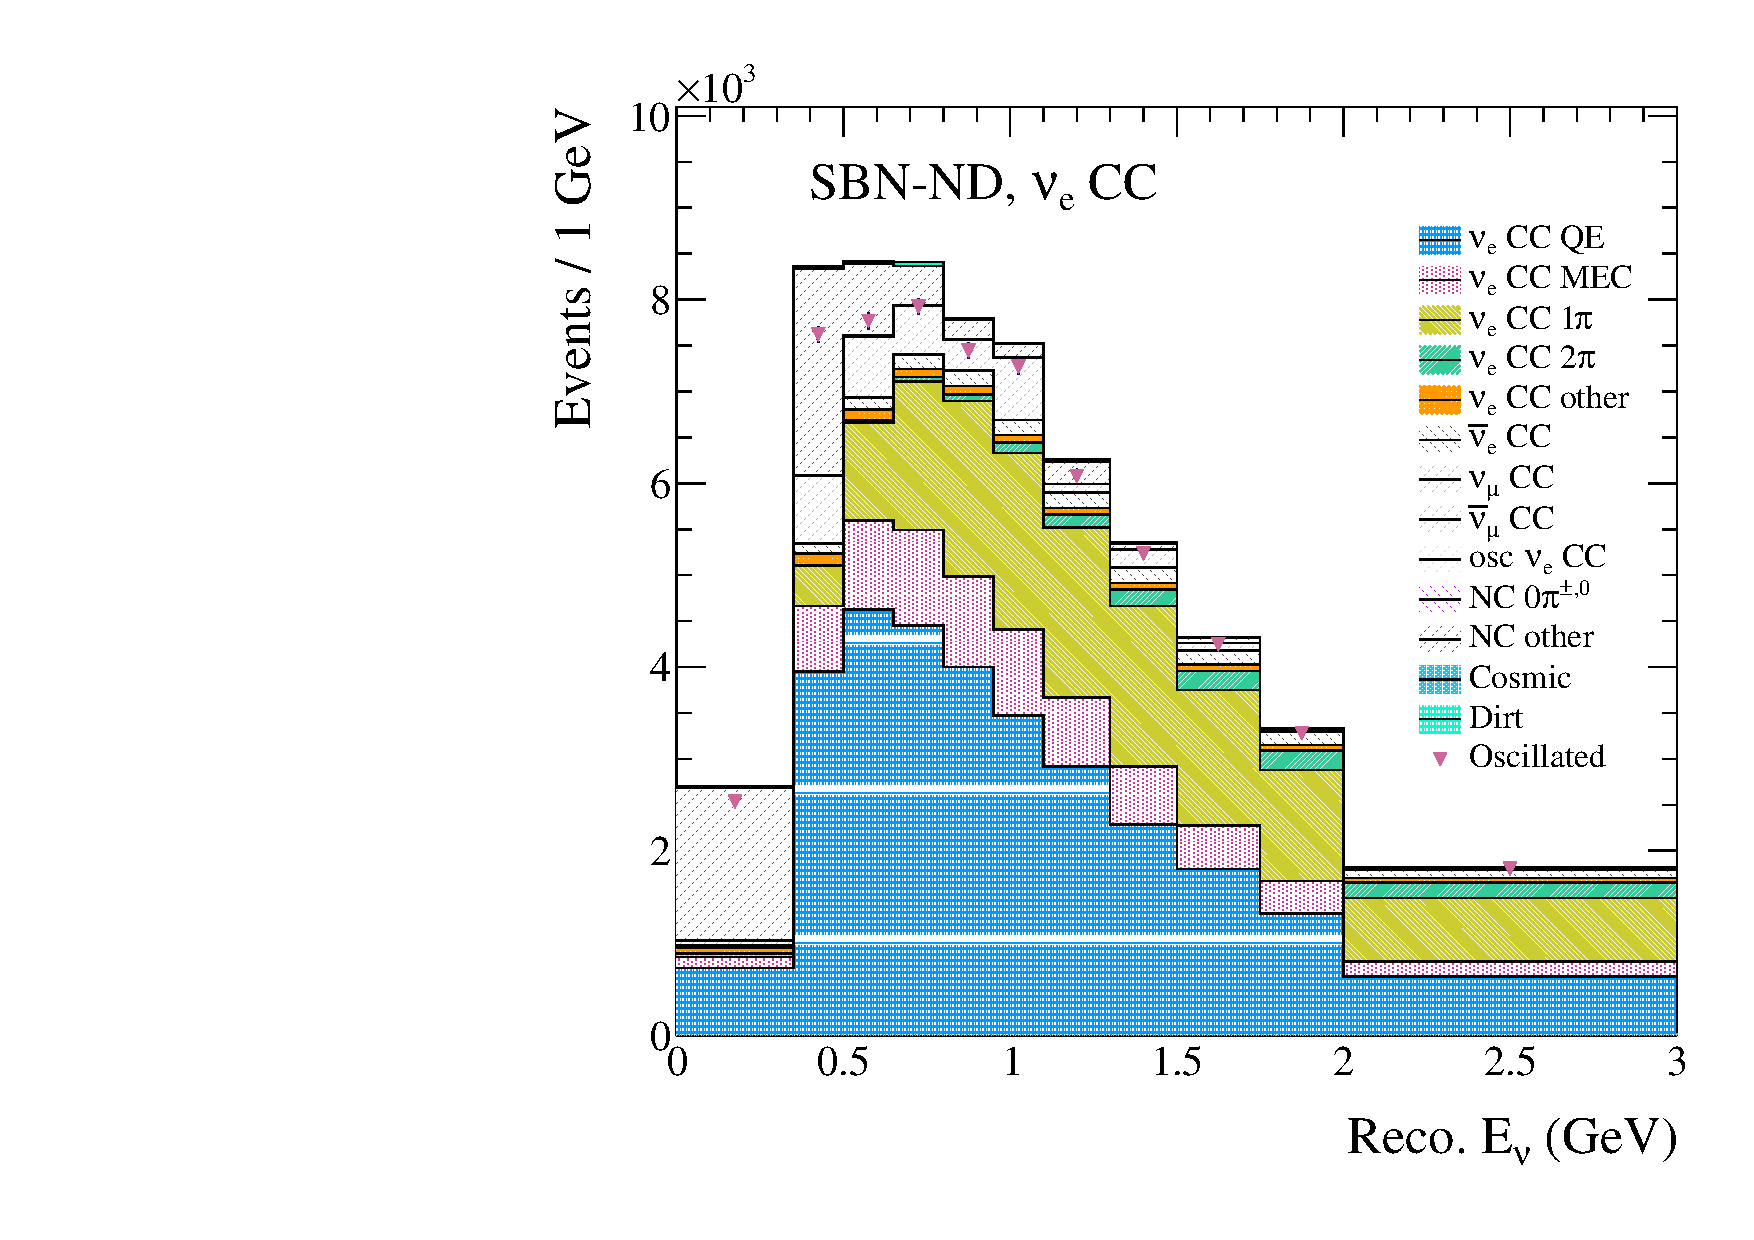
\includegraphics[width=0.49\textwidth]{figures-chap6/spectra/nue_disapp_dmsq_3_sinsq_0.4_overlay_spectrum_sbn_nd_BNB_FHC_0_modes.pdf}}
  {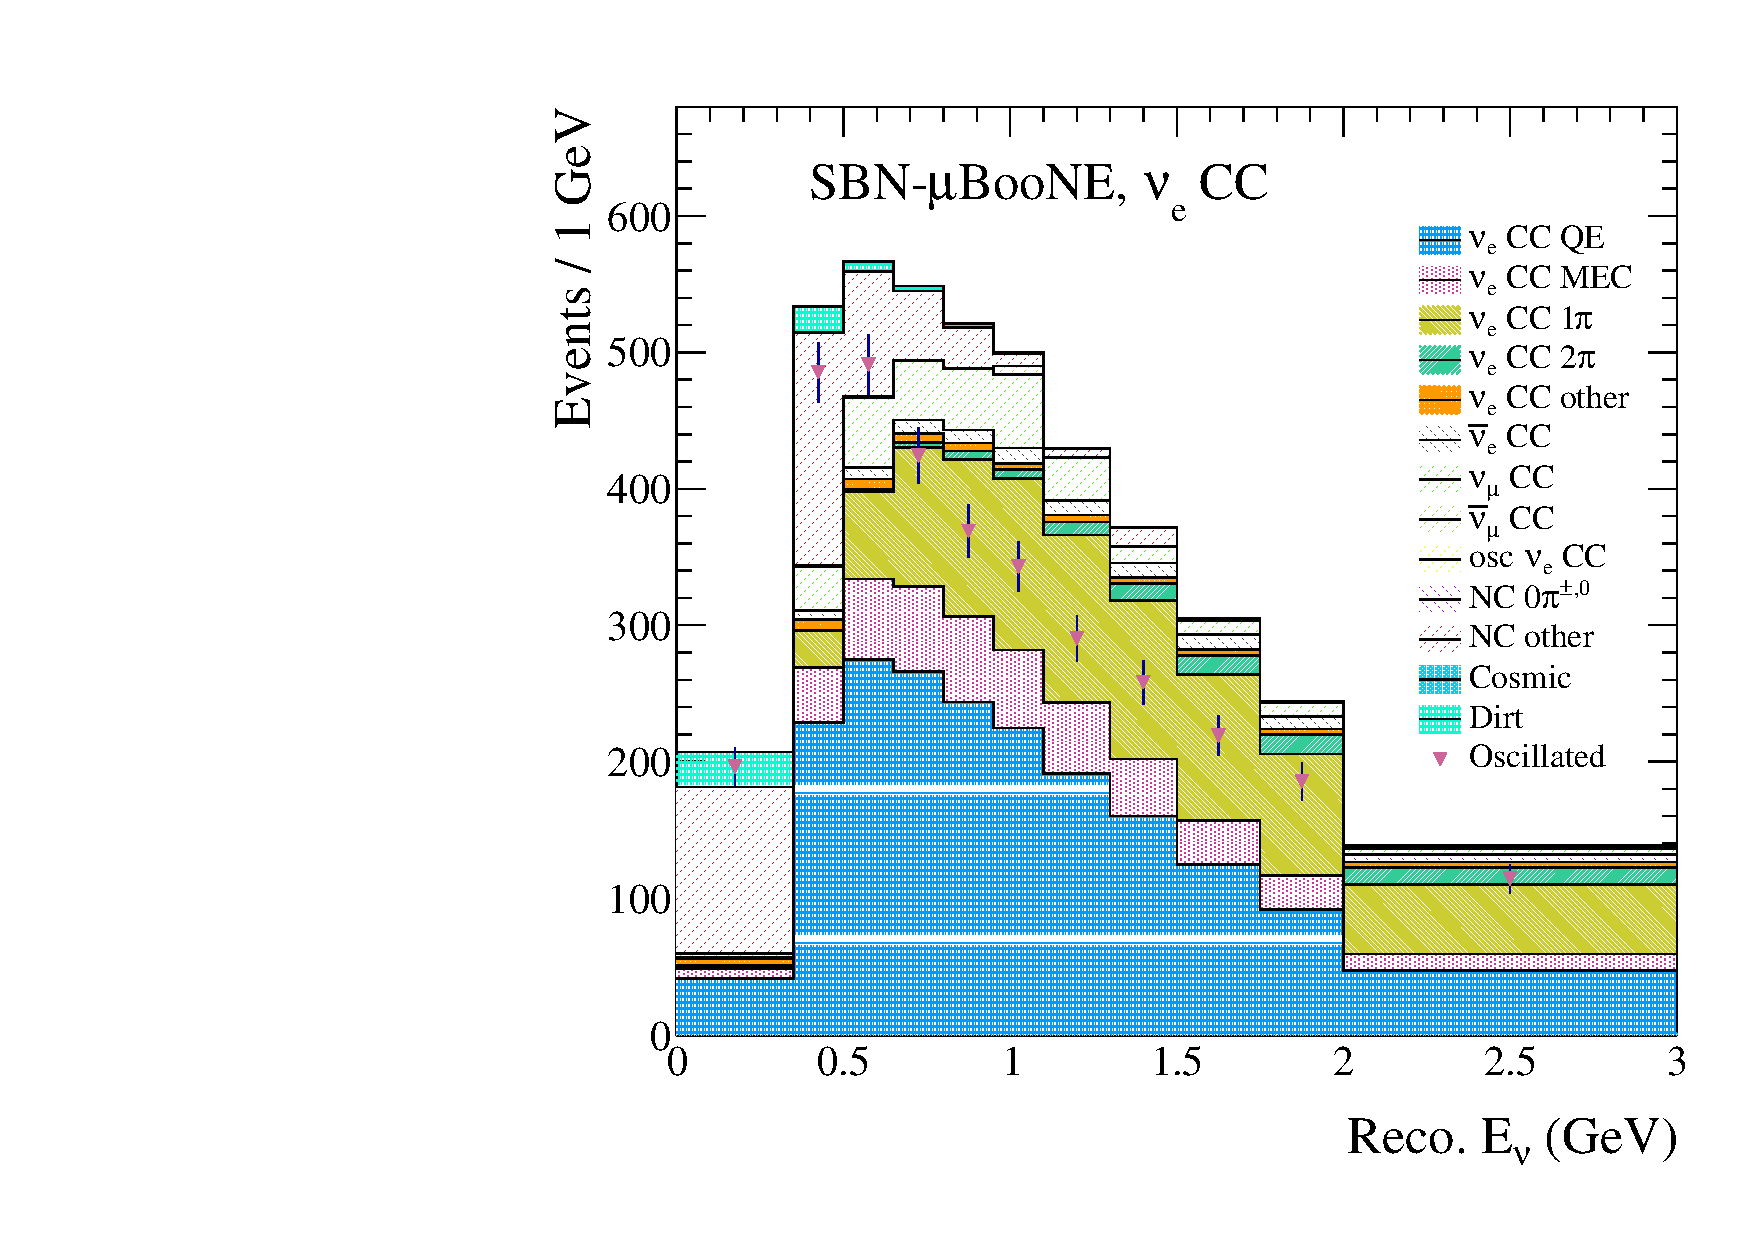
\includegraphics[width=0.49\textwidth]{figures-chap6/spectra/nue_disapp_dmsq_3_sinsq_0.4_overlay_spectrum_sbn_uboone_BNB_FHC_1_modes.pdf}}
  {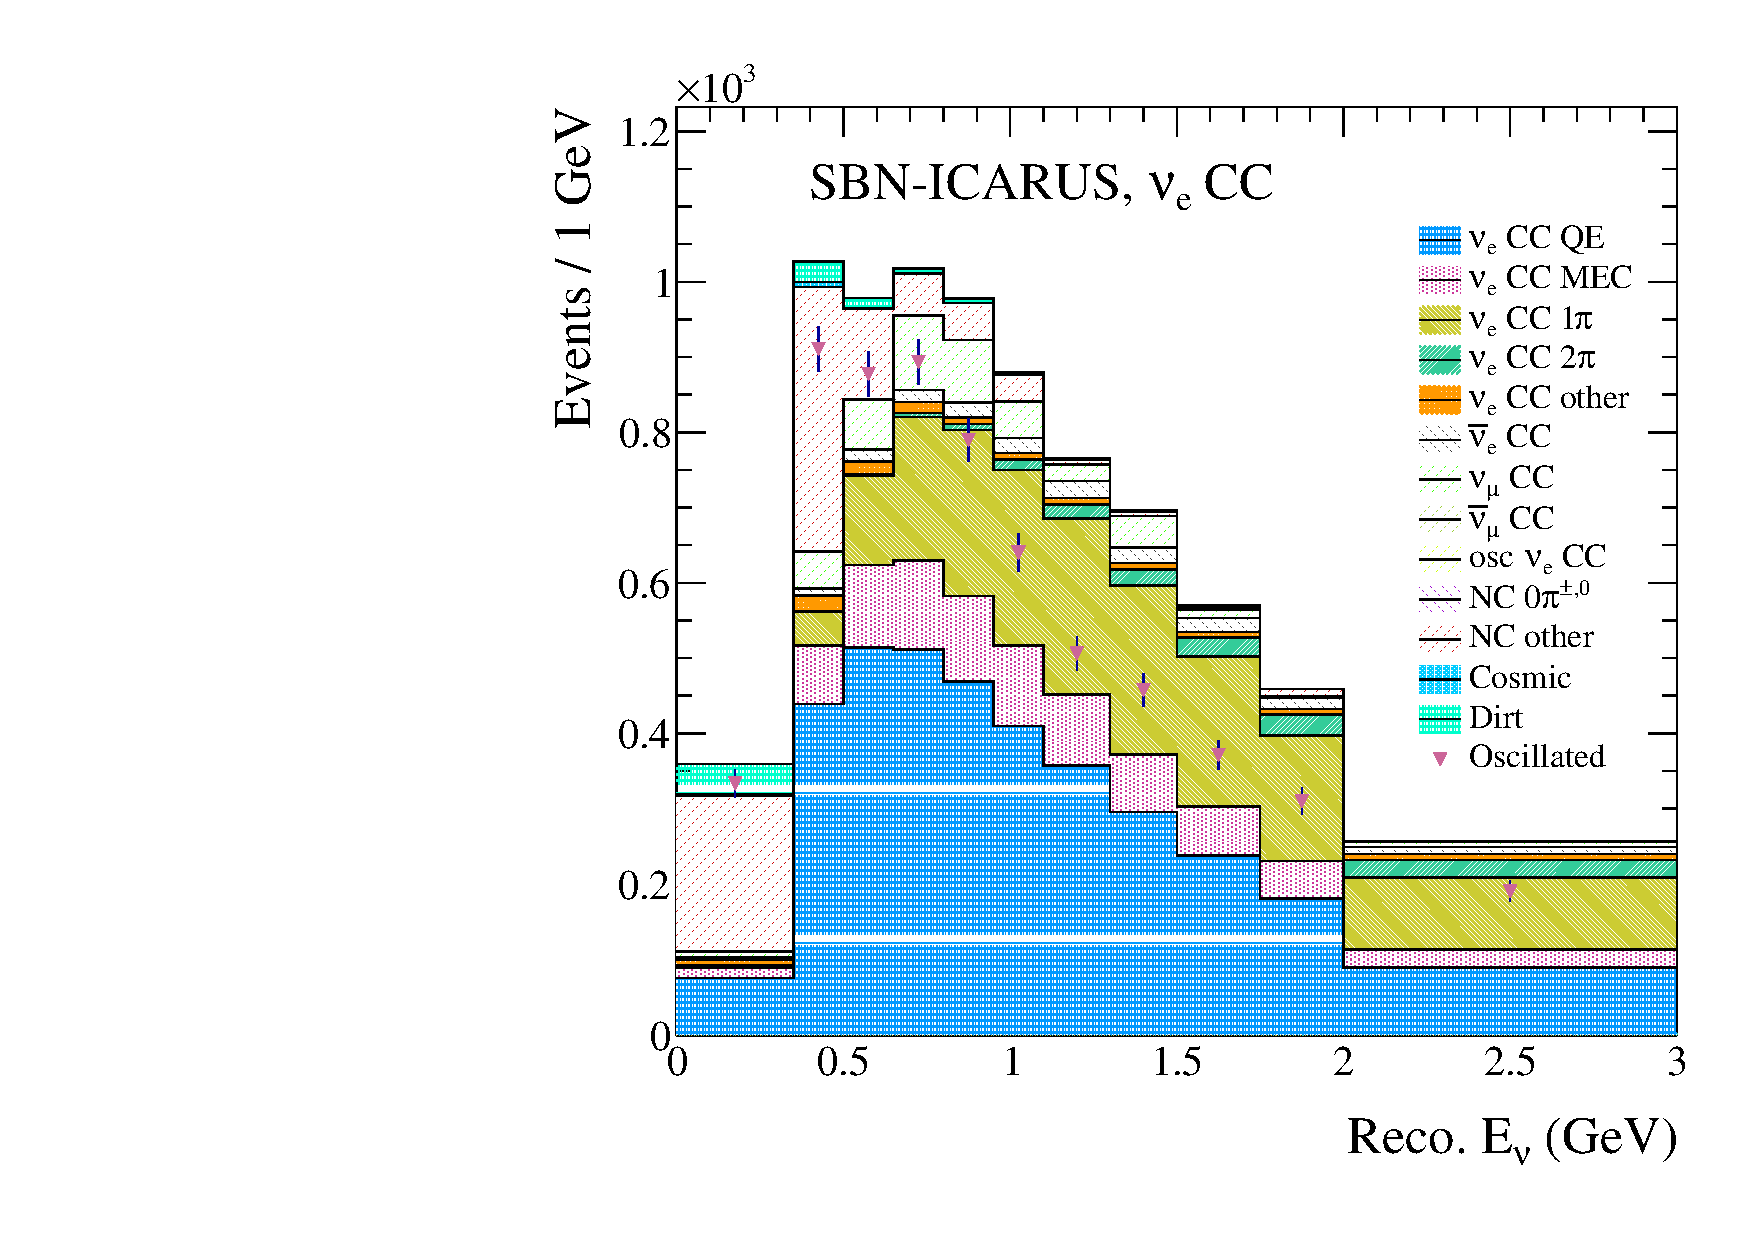
\includegraphics[width=0.49\textwidth]{figures-chap6/spectra/nue_disapp_dmsq_3_sinsq_0.4_overlay_spectrum_sbn_icarus_BNB_FHC_2_modes.pdf}}
  \captionsetup{width=0.49\textwidth}
  \parbox[b]{0.49\textwidth}%
  {
    \caption[SBN \nue disappearance \gls{cc} inclusive reconstructed neutrino energy spectra with oscillated spectrum overlaid.]{The nominal spectra as in \FigureRef{fig:nominal_nue_spectra} but an additional integrated oscillated spectrum with oscillation parameters, $\sin^2{2\theta_{ee}} = 0.4$ and $\Delta m^2_{41} = 3$ eV$^2$ has been overlaid which shows the decrease in event rate.\\\phantom{.}\\\phantom{.}\\\phantom{.}\\}
    \label{fig:nue_disapp_spectra} 
  }
\end{figure}

The top left plot of Figure~\ref{fig:nue_disapp_spectra_ratios} shows the \nue disappearance statistical only exclusion contour and allowed region from fits combining all three \gls{sbn} detectors. The injected point \mbox{$\Delta m^2_{41} = 3$~eV$^2$}, $\sin^2{2\theta_{\mu e}} = 0.4$, used when producing the allowed region is shown along with two further points on the exclusion contour at \mbox{$\Delta m^2_{41} = 1$ eV$^2$}, $\sin^2{2\theta_{\mu e}} = 0.29$ and $\Delta m^2_{41} = 100$~eV$^2$, $\sin^2{2\theta_{\mu e}} = 0.085$. \nue disappearance spectra are produced using oscillation parameters corresponding to each of these three points for each of the three SBN detectors. The ratio of each of these oscillated spectra to the nominal for each detector are shown in the remaining plots in Figure~\ref{fig:nue_disapp_spectra_ratios} and highlight the expected oscillation signal.

\begin{figure}[h!]
    \centering
    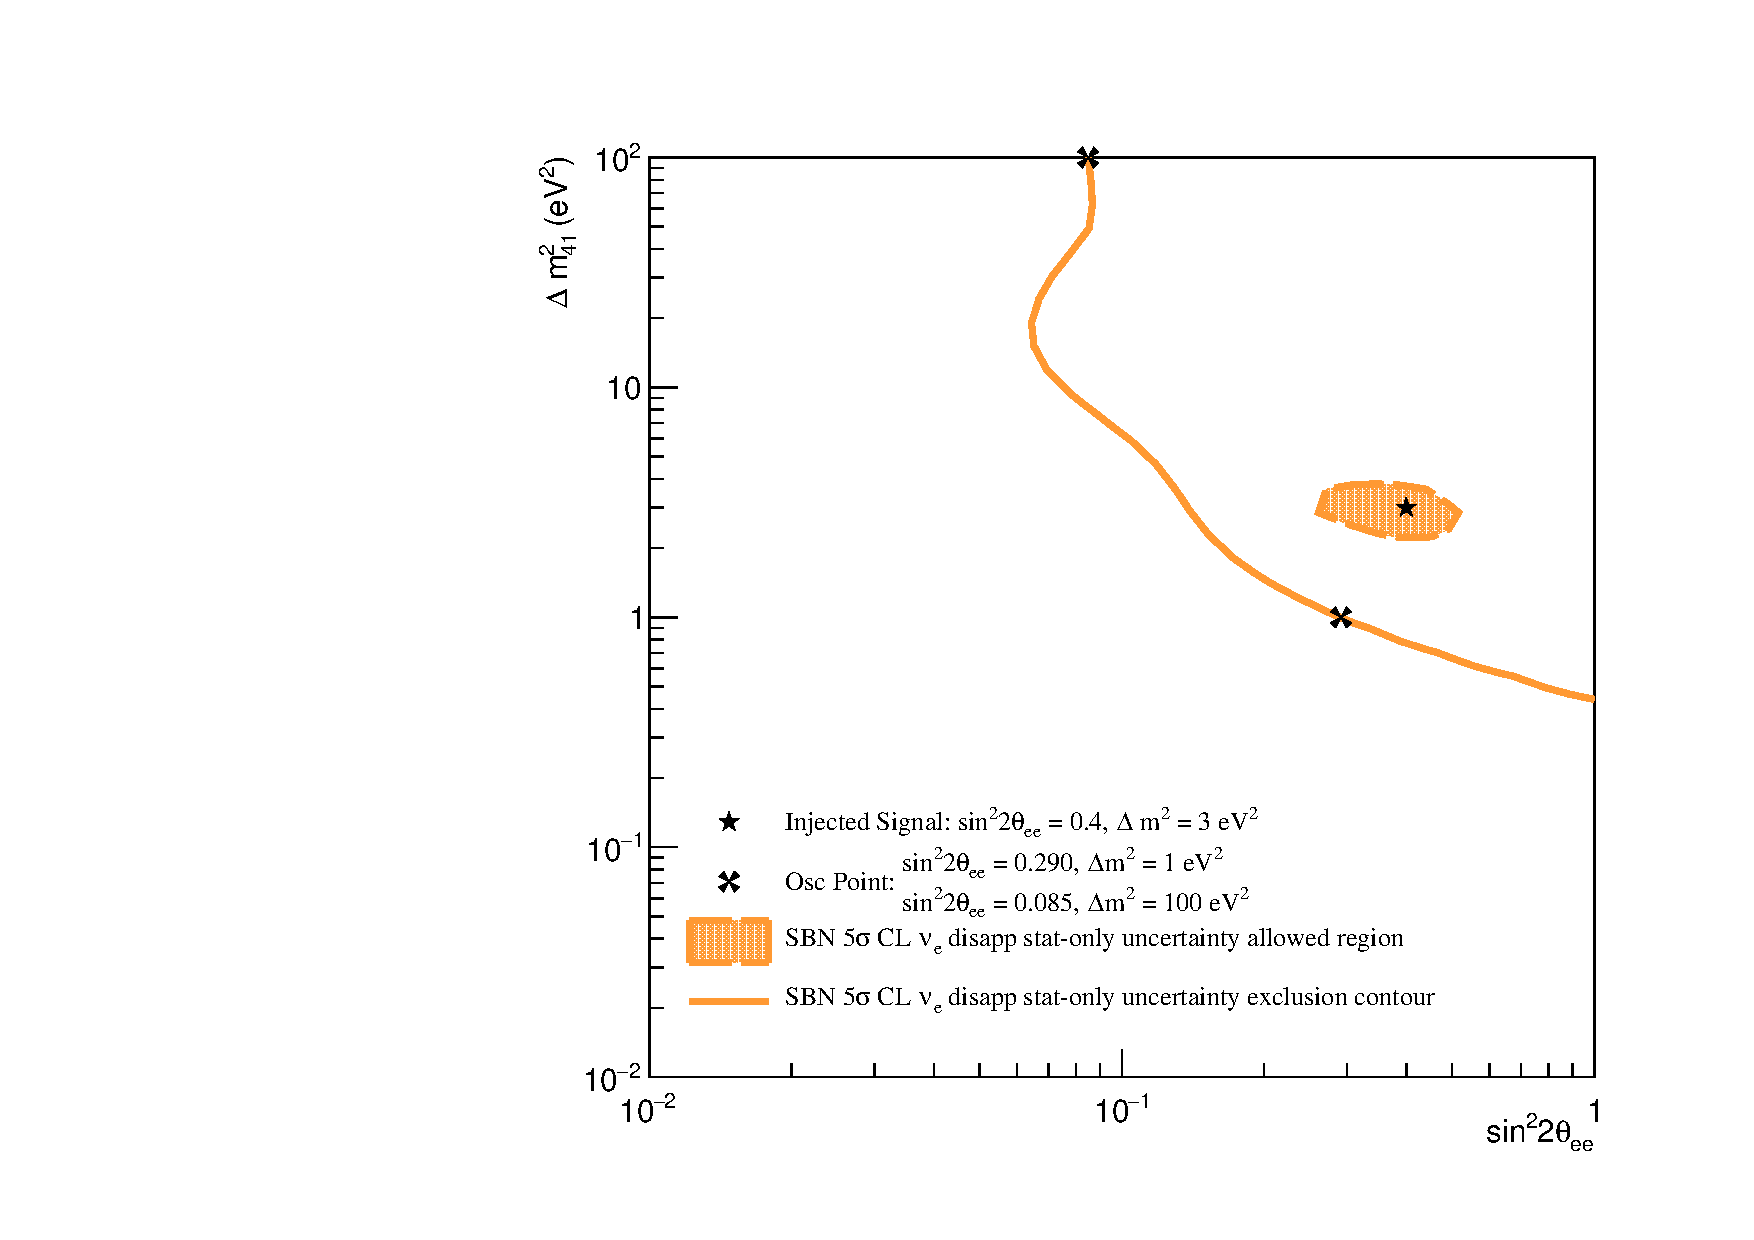
\includegraphics[width = 0.49\textwidth]{figures-chap6/overlays/nue_disapp_stat_osc_markers.pdf}
    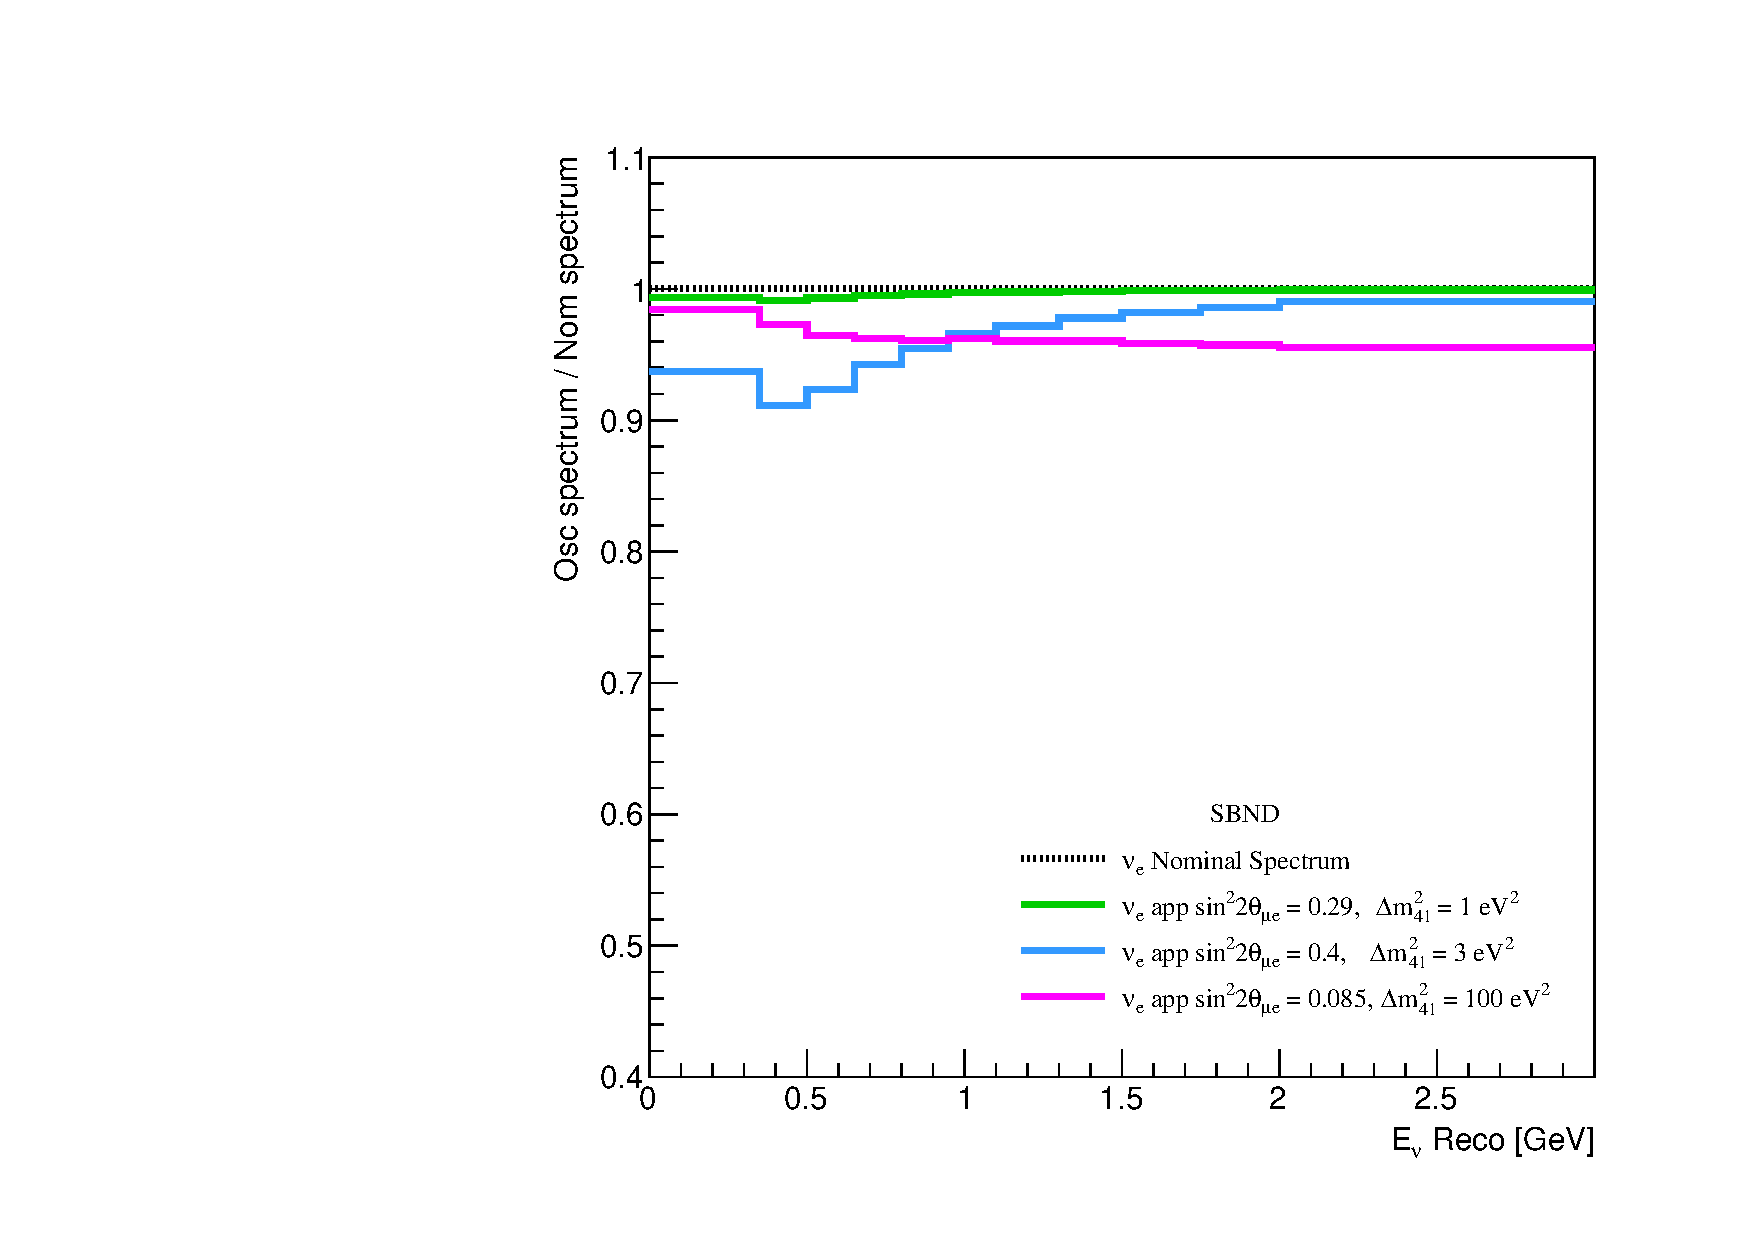
\includegraphics[width = 0.49\textwidth]{figures-chap6/spectra/nue_disapp_spectra_ratio_sbnd.pdf}
    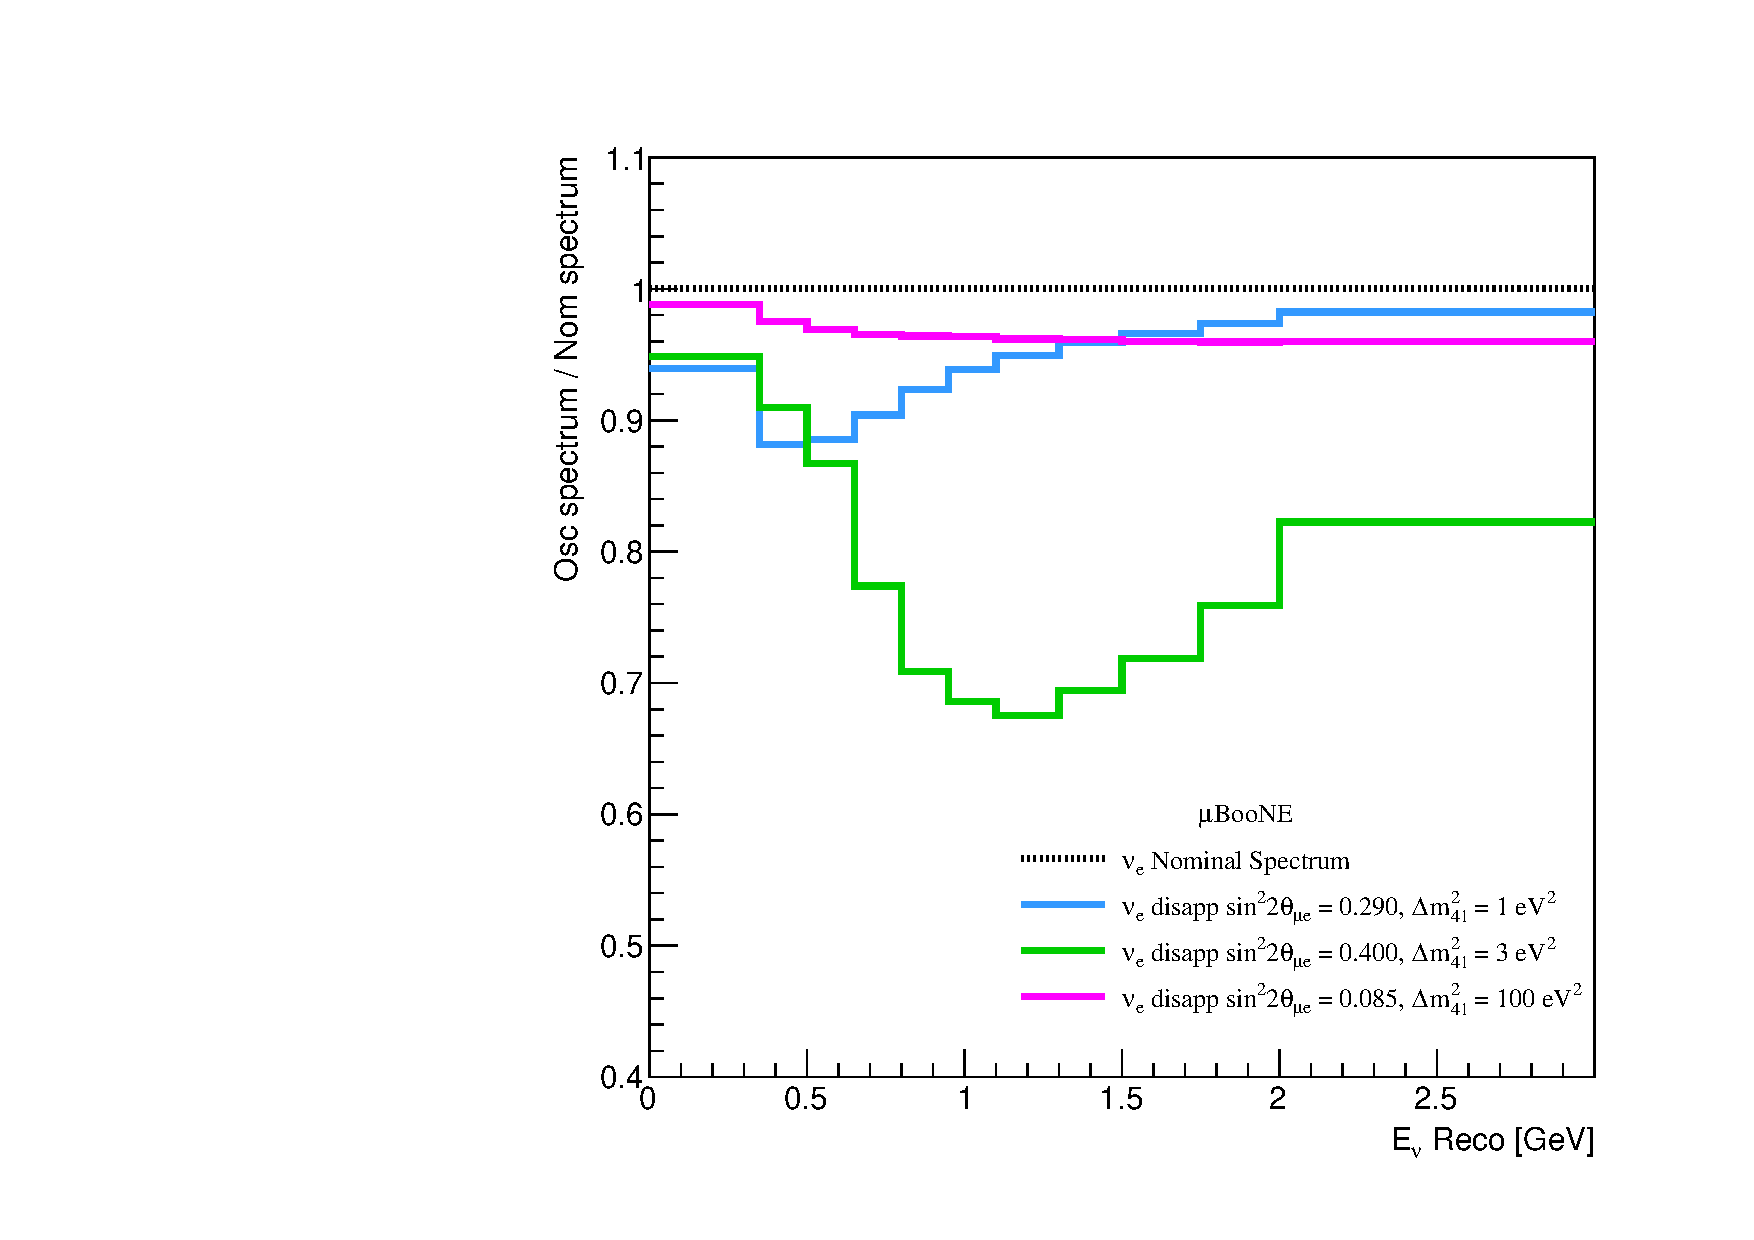
\includegraphics[width = 0.49\textwidth]{figures-chap6/spectra/nue_disapp_spectra_ratio_uboone.pdf}
    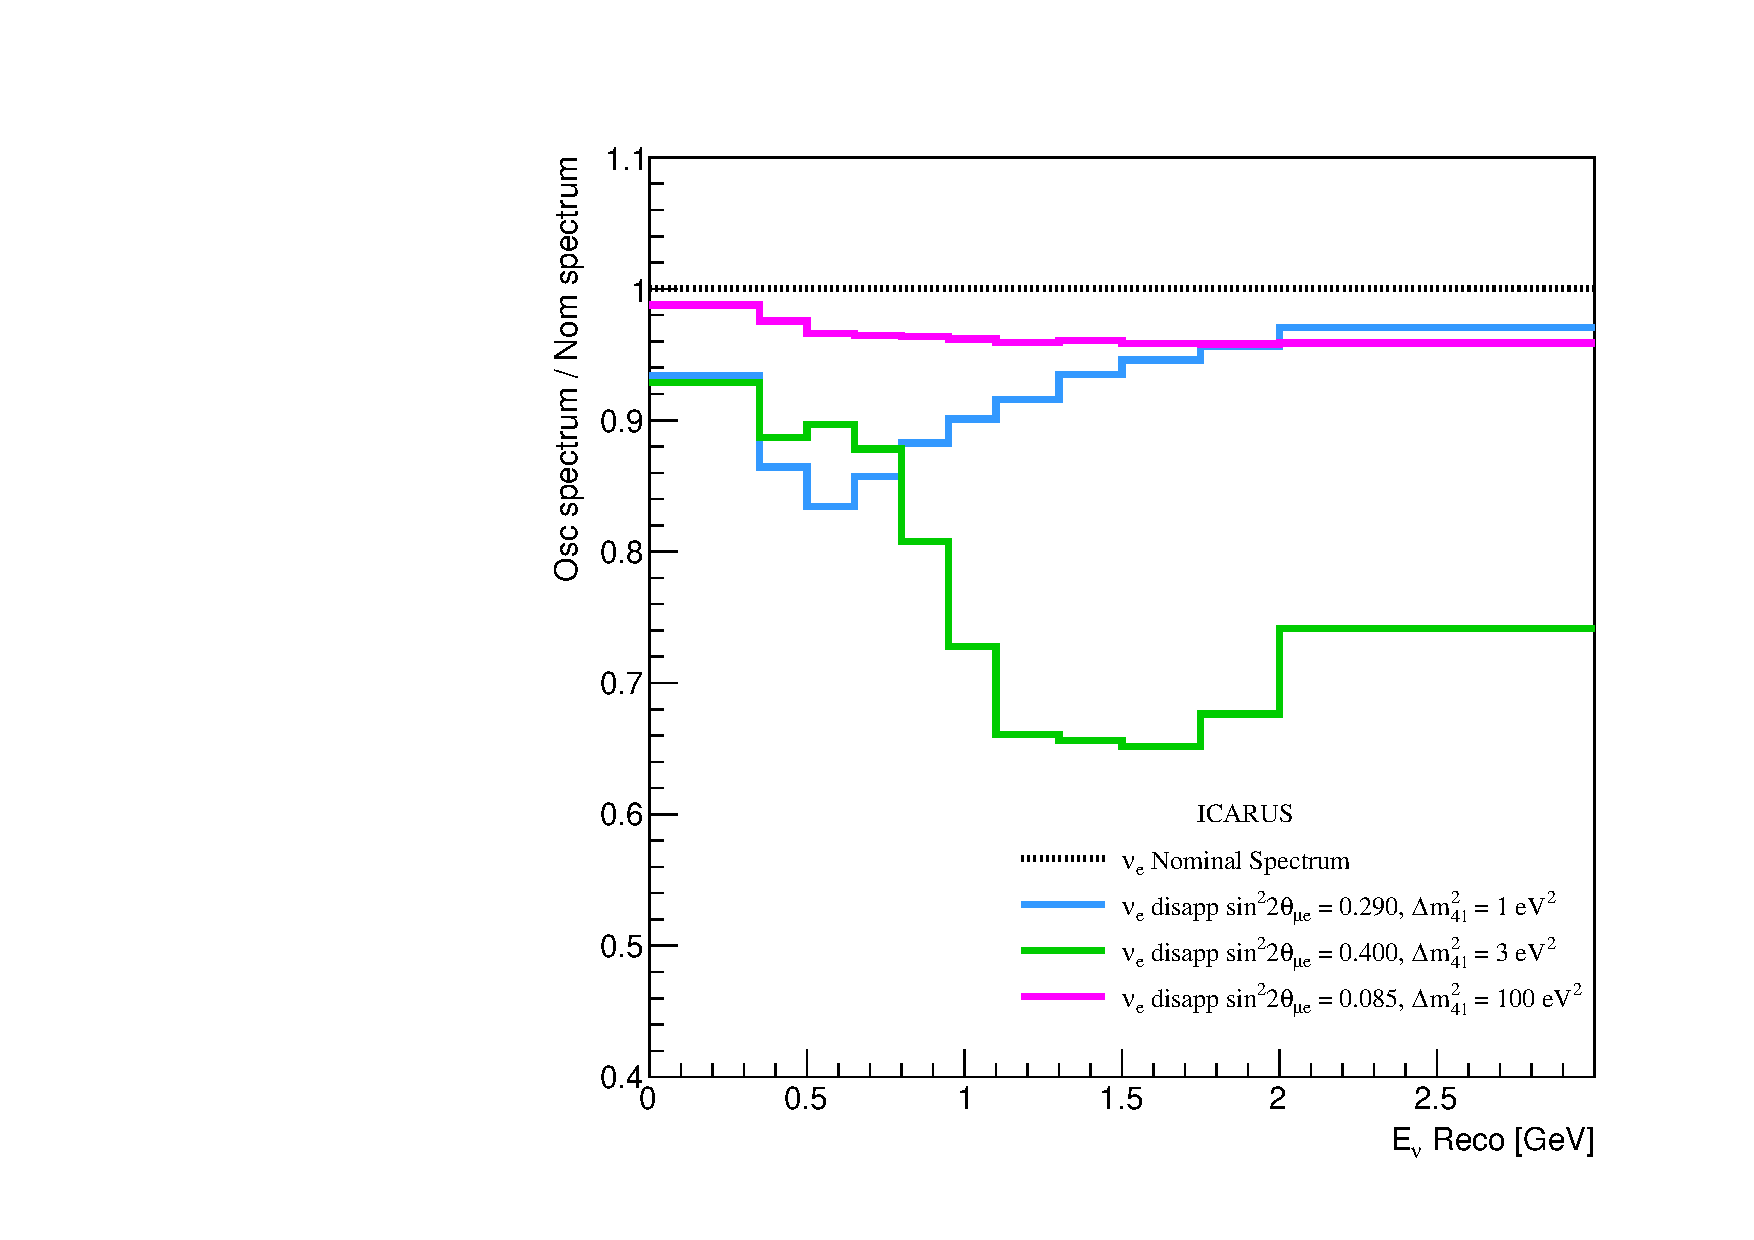
\includegraphics[width = 0.49\textwidth]{figures-chap6/spectra/nue_disapp_spectra_ratio_icarus.pdf}
    \caption[Ratio of \nue disappearance spectra with the oscillation parameters shown on the statistical only contour.]{\nue disappearance stat-only exclusion contour and allowed region. The injected point at $\sin^2{2\theta_{ee}} = 0.4$, $\Delta m^2_{41}$ = 3 eV$^2$ used for the allowed region is shown along with two further points at $\sin^2{2\theta_{ee}} = 0.29$, $\Delta m^2_{41}$ = 1 eV$^2$ and \mbox{$\sin^2{2\theta_{ee}} = 0.085$}, \mbox{$\Delta m^2_{41}$ = 100 eV$^2$} (top left). The ratio of spectra with oscillation parameters corresponding to the three points mentioned versus nominal are shown for \gls{sbnd} (top right), \gls{microboone} (bottom left) and \gls{icarus} (bottom right).}
    \label{fig:nue_disapp_spectra_ratios}
\end{figure}



\clearpage
\section{Sensitivities Studies}\label{sec:sbn_sensitvities}

Following the scheme outlined in \SectionRef{sec:sensitivites_construction}, both allowed and exclusion sensitivity contours are produced for the entire \gls{sbn} program. Additionally, the contribution from individual and combination of detectors on the contours is investigated as well as the impact of different sets of systematic parameters and certain individual parameters. 

%\section{Further Study on Sensitivities}

The sensitivity contours shown in \SectionRef{subsec:evaluation_of_sbn_sensititivites} and \SectionRef{subsec:impact_of_systematic_uncertainties} are produced using the well validated flux and interaction uncertainties, whereas \SectionRef{sec:Impact of Additional Efficiency Systematics} and \SectionRef{subsec:shower_reco_sensitivities} discuss the impact on the exclusion sensitivity contours from the inclusion of additional efficiency uncertainties as well as tweaking the energy smearing used in the event selection based on results from \ChapterRef{chap:Energy_Reco}.

\subsection{\texorpdfstring{Evaluation of SBN Sensitivities for \nue Appearance and Disappearance}{Evaluation of SBN Sensitivities for nue Appearance and Disappearance}}\label{subsec:evaluation_of_sbn_sensititivites}
The complete \nue appearance exclusion sensitivities and allowed regions for both the statistical-only case and with the inclusion of flux and interaction systematics are shown in \FigureRef{fig:nue_app_global_sensitivity} for the entire \gls{sbn} program alongside external limits from the \gls{lsnd} and \gls{karmen} experiments \cite{LSND_KARMEN_nue_app_contour}. For comparison purposes, it should be noted that the contours produced for the \gls{sbn} program are at the $5\sigma$ confidence level whereas the results from both \gls{lsnd} and \gls{karmen} are at the 99\% confidence level. The results from \gls{sbn} shows an improvement over the \gls{karmen} results for essentially all $\Delta m^2_{41}$ values and the allowed region is largely consistent with the \gls{lsnd} result. 


\begin{figure}[h!]
    \centering
    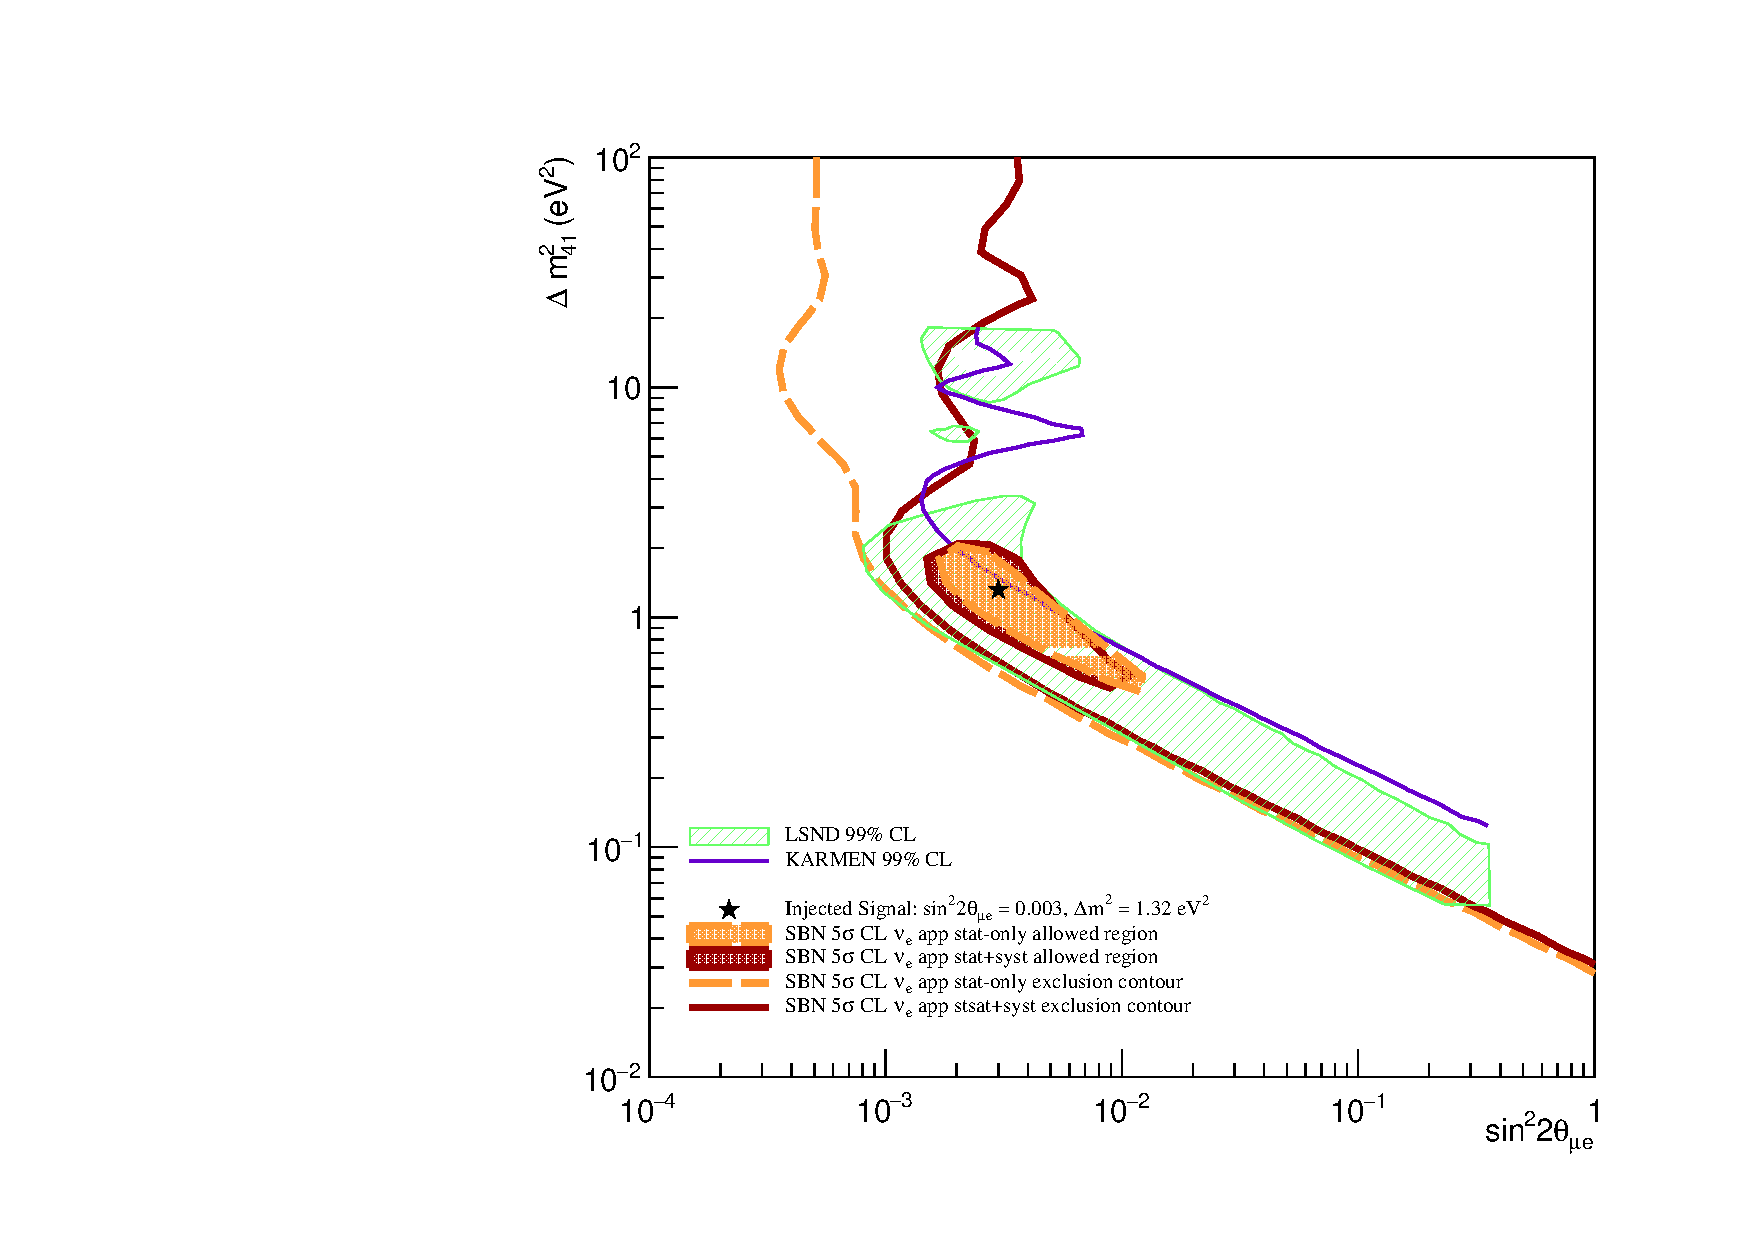
\includegraphics[width = \largefigwidth]{figures-chap6/overlays/valor_overlays_nue_app.pdf}
    \caption[\nue appearance contours with external limits.]{\nue appearance exclusion contours and allowed regions for the stat only case and with flux and interaction systematic uncertainties included. External limits from the \gls{lsnd} and \gls{karmen} experiments have been overlaid \cite{LSND_KARMEN_nue_app_contour}. (The confidence intervals for each contour are shown in the legend and it should be noted that those from external limits are not the same as those from the contours produced for the \gls{sbn} program.)}
    \label{fig:nue_app_global_sensitivity}
\end{figure}

\newpage
The complete \nue disappearance exclusion sensitivities and allowed regions for both the statistical-only case and with the inclusion of flux and interaction systematics are shown in \FigureRef{fig:nue_disapp_global_sensitivity} for the entire \gls{sbn} program alongside external limits from the ND280 detector which serves as one of the near detectors as part of the \gls{t2k} experiment \cite{t2k_experiment}. The results for the \gls{sbn} program are shown at a 5$\sigma$ confidence level whereas the allowed region from the \gls{t2k} experiment is shown at both 68\% and 90\% confidence level and the exclusion contour is at a 95\% confidence level \cite{T2K_nue_disapp_contour}. The results from \gls{sbn} exclude a substantial portion of the \gls{t2k} allowed region with the exclusion limits at high $\Delta m^2_{41}$ not being as strong for the current comparison. 

\begin{figure}
    \centering
    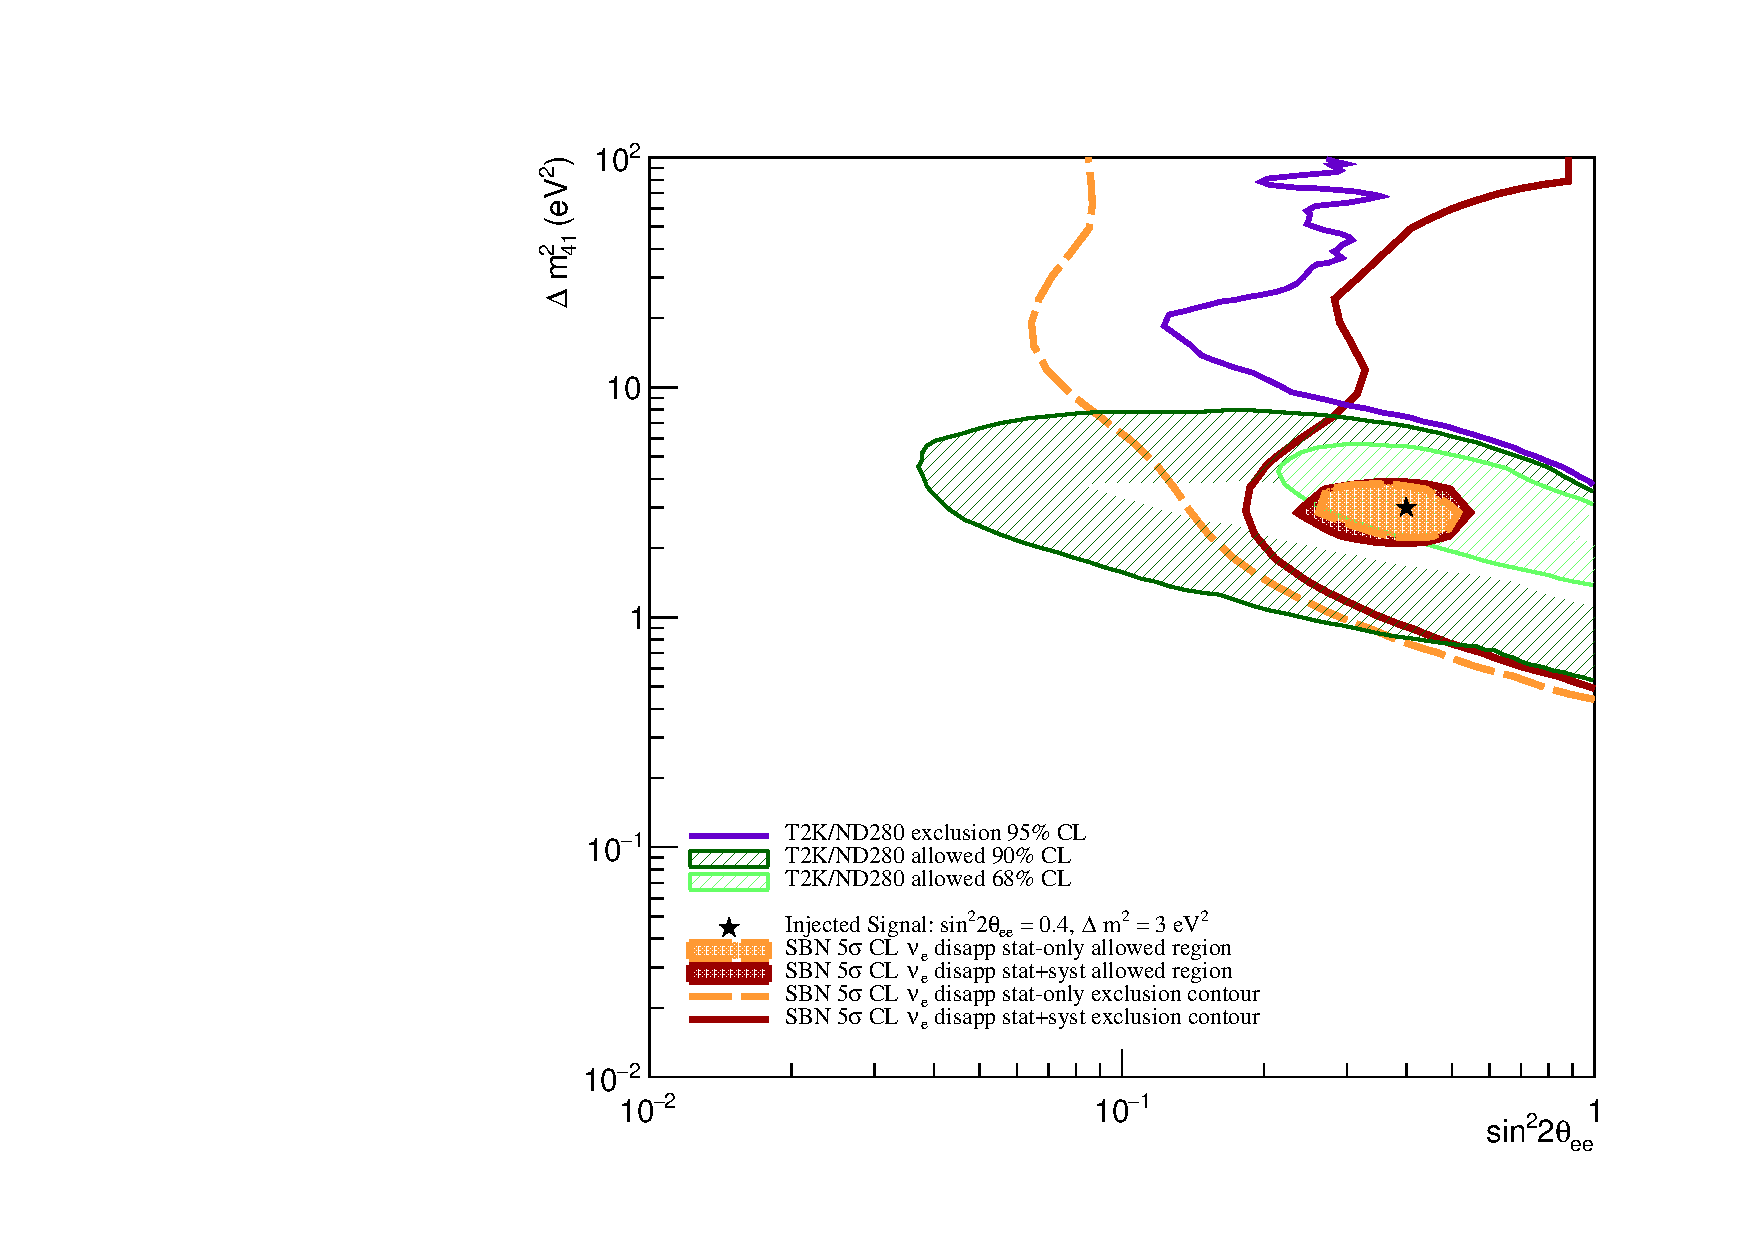
\includegraphics[width = \largefigwidth]{figures-chap6/overlays/valor_overlays_nue_disapp.pdf}
    \caption[\nue disappearance contours with external limits.]{\nue disappearance exclusion contours and allowed regions for the stat only case and with flux and interaction systematic uncertainties included. External limits from the \gls{t2k} experiments have been overlaid \cite{T2K_nue_disapp_contour}. (The confidence intervals for each contour are shown in the legend and it should be noted that those from external limits are not the same as those from the contours produced for the \gls{sbn} program.)}
    \label{fig:nue_disapp_global_sensitivity}
\end{figure}

%\subsection{Impact of Detector Combinations}

To see the impact that each detector has on the sensitivity contour, the left plot of \FigureRef{fig:nue_sensitivity_detector_contribution} shows the \nue appearance statistical-only sensitivity contours from each individual detector as well as all possible combinations (the black curve labelled ``SBN'' refers to a contour from combining all three detectors). It can be seen that for large $\Delta m^2_{41}$ (greater than $\sim$5 eV$^2$), that the \gls{sbnd} detector dominates the sensitivity whereas for small $\Delta m^2_{41}$ (less than $\sim$0.7 eV$^2$) the \gls{icarus} detector dominates. It should also be noted that only by combining the fits from all three detectors can the best sensitivities be obtained. Having this multi-detector design is one of the key advantages of the \gls{sbn} program. The right plot of \FigureRef{fig:nue_sensitivity_detector_contribution} is akin to the left one, but with the inclusion of flux and interaction systematics in the fits. Again, the improvements to the sensitivity are highlighted by combining multiple detectors. 

\begin{figure}[h!]
    \centering
    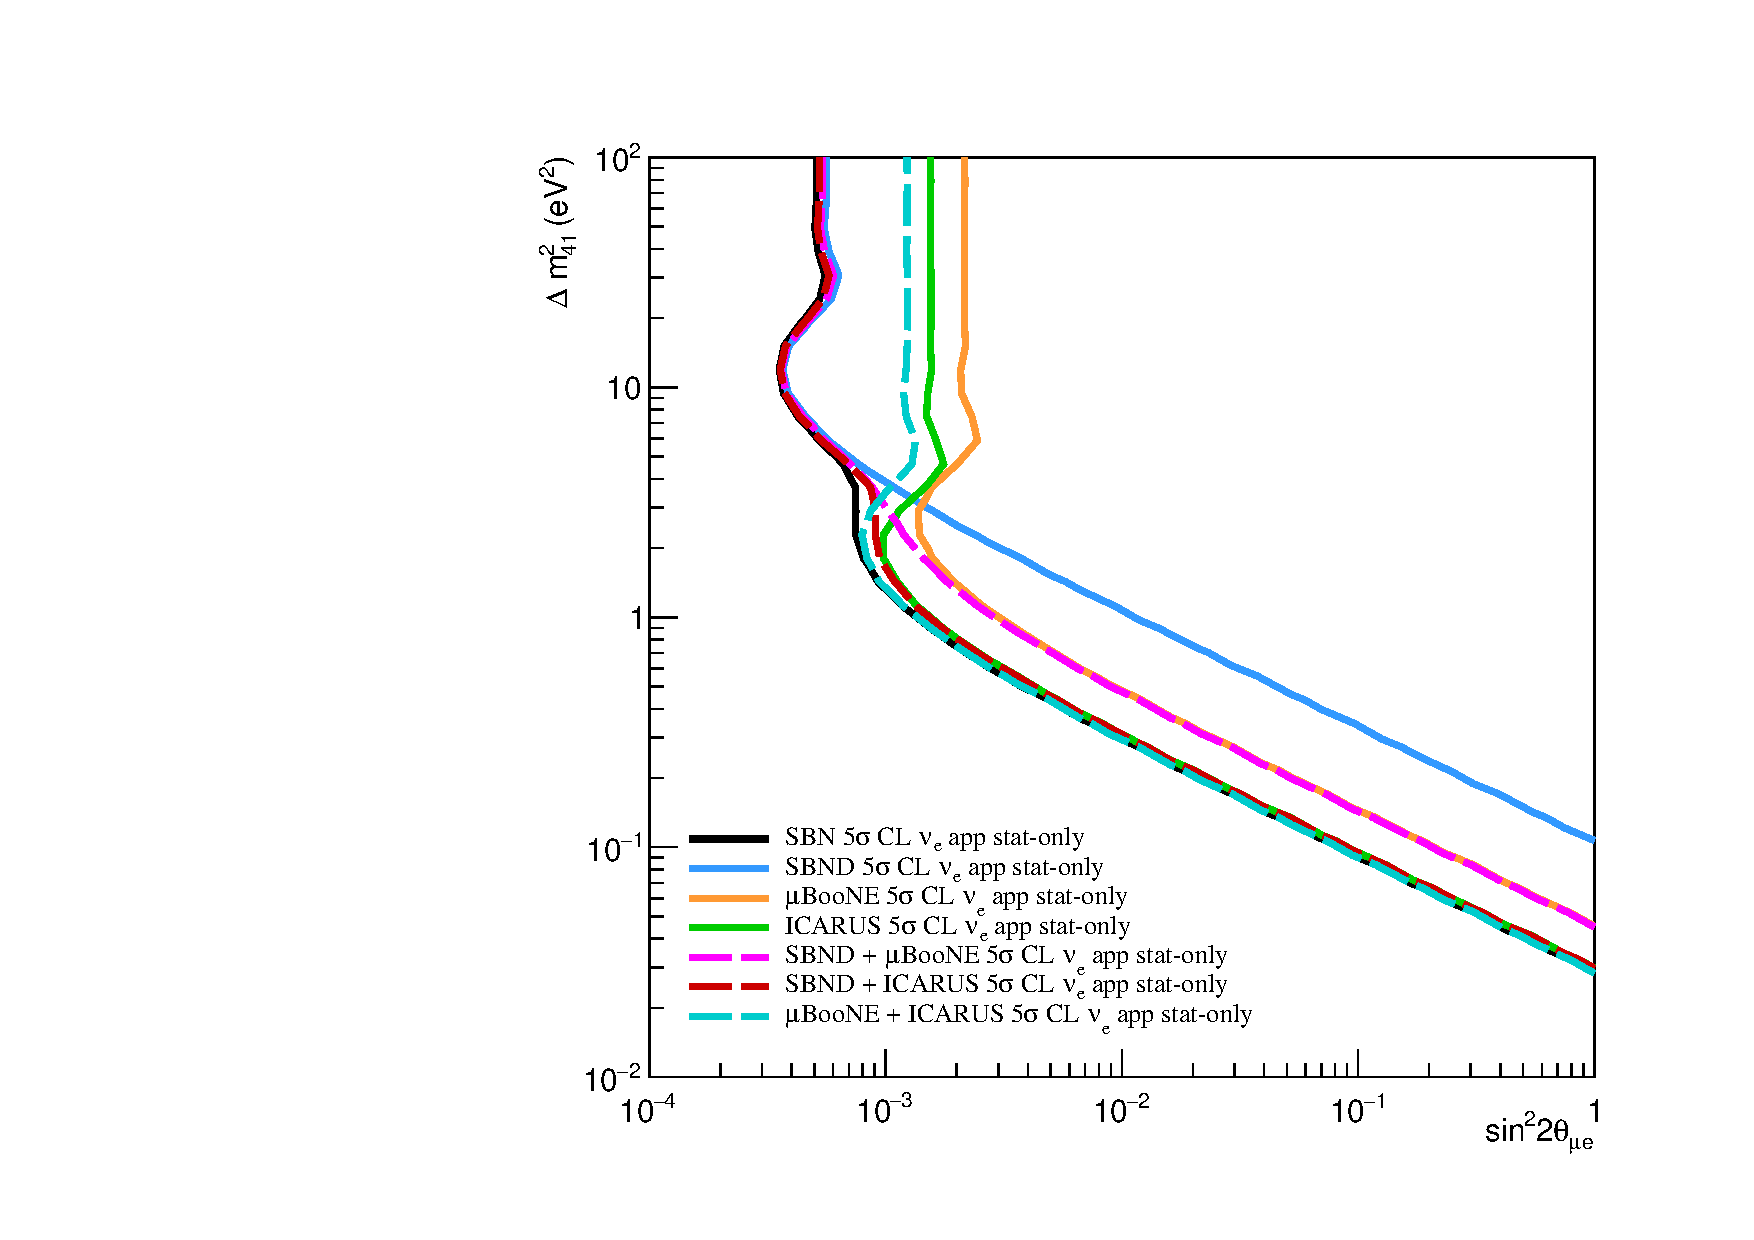
\includegraphics[width = 0.49\textwidth]{figures-chap6/exclusion_contours/nue_app_detector_combinations_stat_only.pdf}
    \includegraphics[width = 0.49\textwidth]{figures-chap6/exclusion_contours/nue_app_detector_combinations_stat+syst.pdf}
    \caption[\nue appearance sensitivities from different detector combinations.]{Contributions to the SBN \nue appearance sterile oscillation sensitivity from each detector and combinations of detectors in the SBN program. The statistical-only plots in the left-hand figure show that SBND is most sensitive to the region $\Delta m_{41}^{2} >$ $\sim$3 eV$^{2}$and ICARUS is most sensitive to $\Delta m_{41}^{2} <$ $\sim$3 eV$^{2}$. The right-hand figure includes flux and interaction systematic parameters and highlights the considerable improvement in the oscillation sensitivity when including multiple detectors in the fits.}
    \label{fig:nue_sensitivity_detector_contribution}
\end{figure}

Similar to \FigureRef{fig:nue_sensitivity_detector_contribution}, \FigureRef{fig:nue_disapp_sensitivity_detector_contribution} shows the \nue disappearance sensitivity from individual detectors and combinations of multiple detectors for both the statistical-only case (Left) and the case with flux and interaction systematics (Right). Again, \gls{sbnd} dominates the sensitivity at high mass splitting whereas \gls{icarus} is dominant for low mass splitting with the emphasis being on the improvement to the overall sensitivity when fits from all three \gls{sbn} detectors are combined.

\begin{figure}[h!]
    \centering
    \includegraphics[width = 0.49\textwidth]{figures-chap6/exclusion_contours/nue_disapp_detector_combinations_stat-only.pdf}
    \includegraphics[width = 0.49\textwidth]{figures-chap6/exclusion_contours/nue_disapp_detector_combinations_stat+syst.pdf}
    \caption[\nue disappearance sensitivities from different detector combinations.]{Contributions to the SBN \nue disappearance sterile oscillation sensitivity from each detector and combinations of detectors in the SBN program produced. The statistical-only plots in the left-hand figure show that SBND is most sensitive to the region $\Delta m_{41}^{2} > 3$~eV$^{2}$ and ICARUS is most sensitive below $\Delta m_{41}^{2} < 3$~eV$^{2}$. The right-hand figure includes flux and interaction systematic parameters and highlights the considerable improvement in the oscillation sensitivity when including multiple detectors in the fits.}
    \label{fig:nue_disapp_sensitivity_detector_contribution}
\end{figure}

\newpage

%\subsection{Impact of Systematic Parameters}

\subsection{Impact of Systematic Uncertainties}\label{subsec:impact_of_systematic_uncertainties}

The impact of systematic sub-groups on the sensitivities are investigated by applying each group in isolation. Following this, the impact of individual systematic parameters on the oscillation parameters is investigated and the dominant uncertainties are identified. The impact of these dominant uncertainties on the sensitivities is then discussed. 

\subsubsection{Impact of Systematic Uncertainty Sub-Groups}
The results from applying the flux, proposal interaction, modern interaction and proposal + modern interaction systematic subgroups for the \nue appearance channel is shown in the left plot of  \FigureRef{fig:nue_app_syst_group_sensitivities}. This highlights the reduction in sensitivity when individually applying each systematic subgroup when compared to the statistical-only case. The right-hand plot of \FigureRef{fig:nue_app_syst_group_sensitivities} shows the ratio of the exclusion contours to the statistical-only case. This gives a clearer measure of the impact on the sensitivity in $\sin^2{2\theta_{\mu e}}$ space. It follows that the interaction systematics have the biggest impact on the sensitivity which in turn are dominated by the modern set of interaction parameters. The proposal set of interaction parameters have the smallest impact with the magnitude of the impact from the flux parameters being somewhere in between the two sets of interaction parameters. 

\begin{figure}[h!]
	\centering
	\includegraphics[width = 0.49\textwidth]{figures-chap6/exclusion_contours/nue_app_syst_groups.pdf}
	\includegraphics[width = 0.49\textwidth]{figures-chap6/exclusion_contours/nue_app_syst_groups_ratios.pdf}
	\caption[Impact of the different systematic parameter groups on the \nue appearance sensitivity.]{The left plot shows the reduction in sensitivity from the stat-only contour when including each set of systematic parameters in the fits. The right plot shows the relative location of each systematic contour in $\sin^{2}2\theta_{\mu e}$ space, with respect to the statistical-only case for the active region of $\Delta m_{41}^{2}$ phase space.}
	\label{fig:nue_app_syst_group_sensitivities}
\end{figure}

The relative contribution of the different systematic groups to the overall exclusion contour for \nue disappearance is shown in \FigureRef{fig:nue_disapp_syst_groups} and is comparable to the \nue appearance case. The interaction systematics again have the largest impact, the majority of which is due to the modern set of parameters. The proposal set of parameters have the smallest impact with the magnitude of the impact from the flux parameters being somewhere in between the two sets of interaction parameters.

\begin{figure}[h!]
	\centering
	\includegraphics[width = 0.49\textwidth]{figures-chap6/exclusion_contours/nue_disapp_syst_groups.pdf}
	\includegraphics[width = 0.49\textwidth]{figures-chap6/exclusion_contours/nue_disapp_syst_groups_ratios.pdf}
	\caption[\nue app sensitivity reduction from different systematic groups.]{The left plot shows the reduction in sensitivity from the stat-only contour when including each set of systematic parameters in the fits. The right plot shows the relative location of each systematic contour in $\sin^{2}2\theta_{ee}$ space, with respect to the statistical-only case for the active region of $\Delta m_{41}^{2}$ phase space.}
	\label{fig:nue_disapp_syst_groups}
\end{figure}

\newpage
\subsubsection{Impact of Individual Systematics}\label{sec:star_plot_study}
%\textcolor{red}{Not sure where best to put this section? Here or along with the sensitivity curves.}

To assess the impact of the different systematic parameters on the oscillation parameters the following study is performed;
\begin{enumerate}
    \item Generate a toy experiment with a given oscillation signal with a single systematic parameter, $f_i$, set to $\pm1\sigma$ from its nominal value and all other systematic parameters are set to their nominal value.
    \item Perform a fit on the toy experiment with $f_i$ fixed to its nominal value. Both the oscillation parameters and all the systematic parameters are initially set to their nominal value and are allowed to float with the exception of $f_i$. The other systematic parameters are allowed to float in order to obtain the best possible agreement between the fit and the toy experiment.
    \item Steps 1. and 2. are then repeated for all \textit{i} systematic parameters of interest. Both the +1$\sigma$ and -1$\sigma$ variations should be performed for each systematic parameter since the effect on the oscillation parameters is typically not symmetric.  
\end{enumerate}
If $f_i$ were allowed to float it would be expected that the fit would be able to recover the same oscillation parameters used in the toy experiment since the same \gls{mc} was used for the toy experiment and the fit. By fixing $f_i$ to its nominal value in the fit, the fit is forced to make a mistake. This results in the fit remapping the changes in $f_i$ to the oscillation parameters (and the other systematic parameters). 

This study was performed for the \nue appearance and disappearance channels using oscillation parameters $\sin^2{2\theta}_{\mu e} = 0.003$, 
$\Delta m^2_{41} = 1.32$ eV$^2$ and 
$\sin^2{2\theta}_{ee} = 0.4$, $\Delta m^2_{41} = 3$ eV$^2$ respectively and includes the results from all uncorrelated systematic parameters. The results are shown in \FigureRef{fig:nue_app_osc_param_pulls} and \FigureRef{fig:nue_disapp_osc_param_pulls}. For both oscillation parameters, the ratio of their value after performing the fit to their nominal value, $\mathcal{R}$, are shown after having varied $f_i$ by $\pm 1 \sigma$. The ratios shown in \FigureRef{fig:nue_app_osc_param_pulls} and \FigureRef{fig:nue_disapp_osc_param_pulls} are always $\geq 1$ by construction since $\mathcal{R}$ is defined as,
\begin{equation}
    \mathcal{R} = \begin{cases}
    \frac{\zeta_{fit}}{\zeta_{nom}}, & \text{if } \zeta_{fit} > \zeta_{nom} \\
    \frac{\zeta_{nom}}{\zeta_{fit}}, &\text{if } \zeta_{nom} > \zeta_{fit},
    \end{cases}
\end{equation}
where $\zeta \in \{\sin^2{2\theta}, \Delta m^2_{41}\}$ and the subscript \textit{nom} and \textit{fit} refer to the nominal value of the oscillation parameters and the values after performing the fit respectively. The arrows are colour coded such that black corresponds to the case where $\zeta_{fit} > \zeta_{nom}$ and red corresponds to the case where $\zeta_{nom} > \zeta_{fit}$.

\begin{figure}[h!]
    \centering
    \includegraphics[width = \textwidth]{figures-chap6/star_plot/nue_app_pulls_2.pdf}
    \caption[\nue appearance oscillation parameter pulls due to varying a single systematic parameter by $\pm1\sigma$.]{The variation in the \nue appearance oscillation parameters due to varying a single systematic parameter at a time by $\pm1\sigma$.}
    \label{fig:nue_app_osc_param_pulls}
\end{figure}

\begin{figure}[h!]
    \centering
    \includegraphics[width = \textwidth]{figures-chap6/star_plot/nue_dsisapp_pulls_2.pdf}
    \caption[\nue disappearance oscillation parameter pulls due to varying a single systematic parameter by $\pm1\sigma$.]{The variation in the \nue disappearance oscillation parameters due to varying a single systematic parameter at a time by $\pm1\sigma$.}
    \label{fig:nue_disapp_osc_param_pulls}
\end{figure}
\clearpage

The impact of the $f_{M_V^{CCRes}}$, $f_{M_A^{CCRes}}$, $f_{R_N^{C Ex}}$ and $f_{\sigma^{\pi}_{INEL}}$ parameters on the \nue appearance exclusion sensitivities are shown in \FigureRef{fig:nue_app_single_param}. The parameters were applied one at a time and chosen as some that showed the largest variations in \FigureRef{fig:nue_app_osc_param_pulls}, ensuring at least one parameter is from each systematic subgroup. Similarly, the $f_{M_V^{CCRes}}$, $f_{M_A^{CCRes}}$, $f_{R_{\pi}^{C Ex}}$ and $f_{expskin}$ parameters were used for the \nue disappearance channel and the results are shown in \FigureRef{fig::nue_disapp_single_param}. Both the statistical-only contour and the one including all the flux and interaction systematics are shown for comparison. It should be noted that single parameters may contribute significantly to the total reduction in sensitivity from the inclusion of all systematic parameters. Additionally, the systematics considered were chosen based on a study which used an injected signal meaning the large impact seen there may not be directly mapped to an exclusion contour which gives a possible reason for the relatively minor impact seen due to $f_{\sigma^{\pi}_{INEL}}$ and $f_{R_{\pi}^{C Ex}}$.

\begin{figure}[h!]
    \centering
    \includegraphics[width = 0.49\textwidth, height = 0.45\textwidth]{figures-chap6/exclusion_contours/single_param/nue_app_single_param.pdf}
    \includegraphics[width =0.49\textwidth, height = 0.45\textwidth]{figures-chap6/exclusion_contours/single_param/nue_app_single_param_ratio.pdf}
    \caption[\nue appearance exclusion contours with the inclusion of a single systematic parameter at a time.]{Left: \nue appearance exclusion contours with the inclusion of a single systematic parameter at a time. The systematic parameters considered are $f_{M_V^{CCRes}}$, $f_{M_A^{CCRes}}$, $f_{R_N^{C Ex}}$ and $f_{\sigma^{\pi}_{INEL}}$. Right: The ratio of the exclusion contours with the inclusion of a single systematic parameter to the statistical-only contour.}
    \label{fig:nue_app_single_param}
\end{figure}

\begin{figure}[h!]
    \centering
    \includegraphics[width = 0.49\textwidth]{figures-chap6/exclusion_contours/single_param/nue_disapp_single_param.pdf}
    \includegraphics[width =0.49\textwidth]{figures-chap6/exclusion_contours/single_param/nue_disapp_single_param_ratio.pdf}
    \caption[\nue disappearance exclusion contours with the inclusion of a single systematic parameter at a time.]{Left: \nue disappearance exclusion contours with the inclusion of a single systematic parameter at a time. The systematic parameters considered are $f_{M_V^{CCRes}}$, $f_{M_A^{CCRes}}$, $f_{R_{\pi}^{C Ex}}$ and $f_{expskin}$. Right: The ratio of the exclusion contours with the inclusion of a single systematic parameter to the statistical-only contour.}
    \label{fig::nue_disapp_single_param}
\end{figure}

\newpage

To further assess the reduction in sensitivities due to specific parameters or parameter groups, allowed regions have been constructed using the same injected signal as was used for the study done to identify the dominant systematics. 
\FigureRef{fig:nue_injected_single_param} shows the change in allowed regions from applying the same set of single systematic parameters for both the \nue appearance and disappearance channels as was done for the exclusion contours. Both the statistical-only contour and the one including flux and interaction systematics have again been included for comparison. 

\begin{figure}[h!]
	\centering
	\includegraphics[width = 0.49\textwidth]{figures-chap6/allowed_regions/single_param/nue_app.pdf}
	\includegraphics[width =0.49\textwidth]{figures-chap6/allowed_regions/single_param/nue_disapp.pdf}
	\caption[\nue appearance and disappearance allowed regions with the inclusion of a single systematic parameter at a time.]{\nue appearance and disappearance allowed regions with the inclusion of a single systematic parameter at a time. The injected signal for \nue appearance is $\sin^2{2\theta_{\mu e}} = 0.003$, $\Delta m^2_{41}$ = 1.32 eV$^2$ whereas the injected signal for \nue disappearance is $\sin^2{2\theta_{ee}} = 0.4$, $\Delta m^2_{41}$ = 3 eV$^2$. The systematic parameters considered for the \nue appearance channel are $f_{M_V^{CCRes}}$, $f_{M_A^{CCRes}}$, $f_{R_N^{C Ex}}$ and $f_{\sigma^{\pi}_{INEL}}$ (Left) and the systematic parameters considered for the \nue disappearance channel are $f_{M_V^{CCRes}}$, $f_{M_A^{CCRes}}$, $f_{R_{\pi}^{C Ex}}$ and $f_{expskin}$ (Right).}
	\label{fig:nue_injected_single_param}
\end{figure}

\newpage
In addition to the exclusion regions, the allowed region with the inclusion of a single parameter are shown along with the corresponding contour from the entire associated set of systematic parameters for the \nue appearance and \nue disappearance channels in \FigureRef{fig:nue_app_single_syst_sets} and \FigureRef{fig:nue_disapp_single_syst_sets} respectively. Unlike for the exclusion contours, the  $f_{\sigma^{\pi}_{INEL}}$ and $f_{R_{\pi}^{C Ex}}$ parameters don't show the smallest change across the entire parameter space. The change is comparable to the other parameters for at least some of the parameter space which is more consistent with the size of the impact seen in the initial study.


\begin{figure}[h!]
  {\includegraphics[width=0.49\textwidth]{figures-chap6/allowed_regions/single_param/nue_app_flux.pdf}}
  {\includegraphics[width=0.49\textwidth]{figures-chap6/allowed_regions/single_param/nue_app_proposal.pdf}}
  {\includegraphics[width=0.49\textwidth]{figures-chap6/allowed_regions/single_param/nue_app_modern.pdf}}
  \captionsetup{width=0.49\textwidth}
  \parbox[b]{0.49\textwidth}%
  {
    \caption[The \nue appearance allowed regions with the inclusion of single systematic parameters compared to the region with the inclusion of all parameters in the associated set.]{The \nue appearance allowed region from an injected signal at $\sin^2{2\theta_{\mu e}} = 0.003$, $\Delta m^2_{41}$ = 1.32 eV$^2$ showing the impact of the $f_{\sigma^{\pi}_{INEL}}$ compared to the total flux systematics (Top Left), the impact of $f_{M_A^{CCRes}}$ compared to the total proposal systematics (Top Right) and the impact of both $f_{M_V^{CCRes}}$ and $f_{R_{\pi}^{C Ex}}$ on the total modern systematics (Bottom Left). The stat only and total flux + interaction contours have been included for comparison. \\}
    \label{fig:nue_app_single_syst_sets} 
  }
\end{figure}

\begin{figure}[h!]
  {\includegraphics[width=0.49\textwidth]{figures-chap6/allowed_regions/single_param/nue_disapp_flux.pdf}}
  {\includegraphics[width=0.49\textwidth]{figures-chap6/allowed_regions/single_param/nue_disapp_proposal.pdf}}
  {\includegraphics[width=0.49\textwidth]{figures-chap6/allowed_regions/single_param/nue_disapp_modern.pdf}}
  \captionsetup{width=0.49\textwidth}
  \parbox[b]{0.49\textwidth}%
  {
  \caption[The \nue disappearance allowed regions with the inclusion of single systematic parameters compared to the region with the inclusion of all parameters in the associated set.]{The \nue disappearance allowed region from an injected signal at $\sin^2{2\theta_{ee}} = 0.4$, $\Delta m^2_{41}$ = 3 eV$^2$ showing the impact of the $f_{expskin}$ compared to the total flux systematics (Top Left), the impact of $f_{M_A^{CCRes}}$ compared to the total proposal systematics (Top Right) and the impact of both $f_{M_V^{CCRes}}$ and $f_{R_N^{C Ex}}$ on the total modern systematics (Bottom Left). The stat only and total flux + interaction contours have been included for comparison. \\}
    \label{fig:nue_disapp_single_syst_sets} 
  }
\end{figure}

\clearpage
\subsubsection{Future Constraints on Systematic Uncertainties}
To further constrain some of the dominant systematic uncertainties in future work a number of options are being considered, which include updated hadron production runs, improvements to \gls{genie} fits and using \gls{sbnd} data.

The NA61/SHINE experiment has already collected data from proton interactions on carbon, beryllium and aluminium with proton momenta of 60 GeV/c and 120 GeV/c (only 60 GeV/c protons were used for the aluminium target) \cite{NA61SHINE}. New runs are being considered using a \gls{bnb}-like target to update the currently available dataset. 

As \gls{genie} continues to be developed, further improvements to interaction models and systematic uncertainty constraints are expected. These may arise from the release of new datasets which will allow for new fits to be performed with inclusion of additional or updated data points. Another possibility is for models to be tuned against exclusive data channels as well as joint exclusive channels in addition to inclusive ones \cite{Julia's_thesis}.
	
Finally, \gls{sbnd} data may also be used to help constrain systematics. This may be achieved, for example, by measuring neutrino-argon interactions with unprecedented statistics or by utilising the \textit{PRISM} concept. The large statistics will allow for the measurement of many different exclusive final state topologies, some of which remain largely unmeasured within argon. An example is the $\nu \electron \rightarrow \nu \electron$ elastic scattering channel. The cross-section of this interaction is well known and the topological signature is easily identifiable in a \gls{lartpc}. For $6.6 \times 10^{20}$ \gls{pot}, \gls{sbnd} expects to observe $\sim 400$ of these events which is sufficient to make a neutrino flux measurement \cite{SBN_paper} \cite{Measurement_of_neutrino_flux_from_neutrino_electron_elastic_scattering}. 

Due to the close proximity of \gls{sbnd} to the neutrino beam source, it is possible to exploit the PRISM effect by considering neutrino interactions as a function of their off-axis angle. As the off-axis angle increases, the peak of the energy spectrum decreases and the overall spectrum becomes narrower. \gls{sbnd}-PRISM may, therefore, measure neutrino interactions at different off-axis angles and deduce the energy dependence on the cross-section over a range of $\sim 200$ MeV. The narrowing of the energy spectrum at larger off-axis angles may also allow certain effects (typically non quasi-elastic) which start to dominate in the $\gtrsim 1$ GeV region to be disentangled from other contributions. 


\subsection{Evaluation of Impact of Efficiency Uncertainties}\label{sec:Impact of Additional Efficiency Systematics}

Efficiency systematics are not implemented in the \textit{standard} analyses because there currently is not a good handle on how to correctly quantify them. A rigorous scheme akin to those described in \SectionRef{sec:flux_syst} and \SectionRef{sec:interaction_syst} does not exist, so instead in-house methods have been developed which are described below.

The current scheme for implementing efficiency (detector) systematics into a fit is by use of a covariance matrix where each element is defined by the systematics outlined in  \TableRef{table:efficiency_systematics}. This allows for the lack of associated event reweighting schemes to be bypassed whilst still being able to capture varying uncertainties being applied to different kinematic ranges, detectors and signal or background processes in each sample. In general, it is assumed that a covariance matrix $\mathcal{M}_{ij}$ is comprised of both correlated and uncorrelated uncertainties such that
\begin{equation}
    \mathcal{M}_{ij} = \mathcal{M}_{ij}^{corr} + \mathcal{M}_{ij}^{uncorr},
\end{equation}
where $\mathcal{M}_{ij}^{corr}$ is the correlated component and $\mathcal{M}_{ij}^{uncorr}$ is the uncorrelated component. For correlated uncertainties,
\begin{equation}
  \mathcal{M}_{ij}^{corr}=\begin{cases}
    \sigma_i^2, & \text{$i = j$}\\
    C_{ij} \sigma_i \sigma_j, & \text{$i \neq j$},
  \end{cases}
\end{equation}
where $C_{ij}$ represents the correlation between the off-diagonal elements and $\sigma_{i,j}$ is some percentage error associated with each systematic. In the case of fully correlated uncertainties, $C_{ij}$ reduces to one and $\sigma_i = \sigma_j$. For uncorrelated uncertainties,
\begin{equation}
  \mathcal{M}_{ij}^{uncorr}=\begin{cases}
    \sigma_i^{\prime2}, & \text{$i = j$}\\
    0, & \text{$i \neq j$},
  \end{cases}
\end{equation}
with $\sigma_i^{\prime}$ again being a percentage error. 
If any correlated errors are assumed to be fully correlated, $\mathcal{M}_{ij}$ will then have diagonal elements given by $\sigma_i^2 + \sigma_i^{\prime2}$ and off-diagonal elements given by $\sigma_i^2$.

\begin{table}[h!]
\begin{adjustbox}{width=\textwidth,center}
	\begin{tabular}{l lllll}
		\hline
		& \multicolumn{5}{c}{\textbf{Applies to}}                                                                                  \\
		\textbf{Systematic}    & \textbf{Beam} & \textbf{Detector} & \textbf{Sample}        & \textbf{Mode} & \textbf{Reco. energy bin edges}                            \\ \hline
		$f_0 - f_7$   & FHC  & SBND     & $\numu$CC-like & signal/$\numu$CC & \{0, 0.2, 0.4, 0.6, 0.8, 1.0, 1.5, 2.0, $\infty$\}      \\
		$f_8 - f_{13}$    & FHC  & SBND     & $\numu$CC-like   & bkg/NC               & \{0, 0.2, 0.4, 0.6, 0.8, 1.0, $\infty$\}                \\
		$f_{14}$          & FHC  & SBND     & $\numu$CC-like   & bkg/Dirt             & \{0, $\infty$\}                                         \\
		$f_{15}$          & FHC  & SBND     & $\numu$CC-like   & bkg/Cosmics          & \{0, $\infty$\}                                         \\ \hline
		$f_{16}-f_{24}$     & FHC  & SBND     & $\nue$CC-like     & signal/$\nue$CC     & \{0, 0.2, 0.4, 0.6, 0.8, 1.0, 1.5, 2.0, 3.0, $\infty$\} \\
		$f_{25} - f_{33}$   & FHC  & SBND     & $\nue$CC-like     & bkg/$\numu$CC      & \{0, 0.2, 0.4, 0.6, 0.8, 1.0, 1.5, 2.0, 3.0, $\infty$\} \\
		$f_{34} - f_{42}$   & FHC  & SBND     & $\nue$CC-like     & bkg/NC1$\gamma$        & \{0, 0.2, 0.4, 0.6, 0.8, 1.0, 1.5, 2.0, 3.0, $\infty$\} \\
		$f_{43} - {f_51}$   & FHC  & SBND     & $\nue$CC-like     & bkg/NC1$\pi^0$         & \{0, 0.2, 0.4, 0.6, 0.8, 1.0, 1.5, 2.0, 3.0, $\infty$\} \\
		$f_{52} - f_{60}$   & FHC  & SBND     & $\nue$CC-like     & bkg/NCother          & \{0, 0.2, 0.4, 0.6, 0.8, 1.0, 1.5, 2.0, 3.0, $\infty$\} \\
		$f_{61} - f_{66}$   & FHC  & SBND     & $\nue$CC-like     & bkg/Dirt             & \{0, 0.2, 0.4, 0.6, 0.8, 1.0, $\infty$\}                \\
		$f_{67} - f_{72}$   & FHC  & SBND     & $\nue$CC-like     & bkg/Cosmics          & \{0, 0.2, 0.4, 0.6, 0.8, 1.0, $\infty$\}                \\ \hline
		$f_{73} - f_{145}$  & \multicolumn{5}{l}{As above, but for $\mu$B}                                                                        \\ \hline
		$f_{146} - f_{218}$ & \multicolumn{5}{l}{As above, but for ICARUS}                                                                    \\ \hline
	\end{tabular}
\end{adjustbox}
\caption[Binning scheme for the efficiency uncertainties.]{The binning scheme used to produce the efficiency uncertainty covariance matrices.}
\label{table:efficiency_systematics}
\end{table}

All future discussion involving correlated uncertainties should from here on be assumed to be fully correlated even if not explicitly stated. A set of example covariance matrices are shown in \FigureRef{fig:efficiency_cov_matrices}. The top left plot corresponds to a 10\% correlated error only. The remaining three plots all have a correlated error of 2\%, with some varying amounts of an uncorrelated error associated with each systematic. 

\begin{figure}[h!]
    \centering
    \includegraphics[width = 0.49\textwidth]{figures-chap5/efficiency_matrices/efficiency_error_matrix_48x48_type1_cor10.00pct.root.pdf}
    \includegraphics[width = 0.49\textwidth]{figures-chap5/efficiency_matrices/efficiency_error_matrix_48x48_type2_cor2.00pct_sbnduncor1.00pct_ubooneuncor1.00pct_icarusuncor1.00pct.root.pdf}
    \includegraphics[width = 0.49\textwidth]{figures-chap5/efficiency_matrices/efficiency_error_matrix_48x48_type2_cor2.00pct_sbnduncor2.00pct_ubooneuncor0.50pct_icarusuncor0.50pct.root.pdf}
    \includegraphics[width = 0.49\textwidth]{figures-chap5/efficiency_matrices/efficiency_error_matrix_48x48_type3_cor2.00pct_bulkuncor0.50pct_allpeakEnumuCCuncor2.00pct.root.pdf}
    \caption[Example efficiency uncertainty covariance matrices.]{Covariance matrices produced to investigate the effects of efficiency systematics for the \numu disappearance channel. Top left: A 10\% fully correlated error only. Top right: A 2\% fully correlated error with an additional 1\% uncorrelated error across all bins. Bottom left: A 2\% fully correlated error with an additional 2\% uncorrelated error for all \gls{sbnd} bins and a 0.5\% uncorrelated error for all \gls{microboone} and \gls{icarus} bins. Bottom right: A 2\% fully correlated error with an additional 2\% uncorrelated error for the peak energy bins (0.6 - 1.0 GeV) in each detector and a 0.5\% uncorrelated error for all other bins.}
    \label{fig:efficiency_cov_matrices}
\end{figure}

\newpage
In order to get a measure of the possible impact of efficiency systematics on the sensitivity, various covariance matrices were produced to investigate the impact of:
\begin{enumerate}
    \item Fully correlated errors only.
    \item Various combinations of uncorrelated errors with a fixed correlated error.
    \item Uncorrelated errors only applied to a single detector at a time.
    \item A poorly constrained uncorrelated error on a single set of bins.
\end{enumerate}
Unless otherwise stated, the uncertainties from efficiency covariance matrices are applied in addition to the flux and interaction systematics. 

The study on the impact of different efficiency uncertainties was first done for the \numu disappearance channel because it was expected that there would be a greater impact than for either of the \nue channels. This is because the typical event rate for the \numu channel is several orders of magnitude greater than that of \nue meaning that the \numu channel is systematics limited whereas the \nue channels may tend towards being statistics limited. Once a contour becomes statistics limited, continuing to apply additional systematic uncertainties will begin to have diminishing impacts. 

Sensitivities including efficiency uncertainties for the \numu disappearance channel are shown alongside the other figures in \AppendixRef{app:numu_disapp}. The impact of the efficiency uncertainties on both \nue channels is discussed below.


\subsubsection*{\texorpdfstring{Impact of Efficiency Systematics on \nue Appearance Sensitivities}{Impact of Efficiency Systematics on nue Appearance Sensitivities}}

In order to gauge the contribution of some typical efficiency uncertainty, \FigureRef{fig:nue_app_syst_groups+efficiency} shows the impact on the \nue appearance sensitivity from individual sets of systematic parameters as in \FigureRef{fig:nue_app_syst_group_sensitivities} but with the additional case where only a 2\% correlated + 2\% uncorrelated efficiency uncertainty has been applied. The impact of the efficiency uncertainty is comparable to the proposal interaction systematics having the smallest contribution to the sensitivity. 

\begin{figure}[h!]
    \centering
    \includegraphics[width = \largefigwidth]{figures-chap6/exclusion_contours/nue_app_syst_groups+det.pdf}
    \caption[\nue app sensitivity reduction from different systematic groups with a (2+2)\% efficiency uncertainty.]{The reduction in the \nue appearance sensitivity from the stat-only contour when including each set of systematic parameters in the fits. Similar to \FigureRef{fig:nue_app_syst_group_sensitivities} but with the addition of a 2\% correlated and 2\% uncorrelated efficiency uncertainty.}
    \label{fig:nue_app_syst_groups+efficiency}
\end{figure}

The reduction in sensitivity from applying a 10\% correlated uncertainty and a 2\% correlated + 2\% uncorrelated uncertainty on top of the standard flux and interaction systematics are shown in \FigureRef{fig:nue_app_corr_uncorr_error}. Since a correlated error of 10\% has a close to negligible impact, the results from applying correlated uncertainties less than 10\% as was done for the \numu channel have been omitted. Similarly, applying smaller uncorrelated uncertainties would again only have a minor impact so these have also been omitted.  

\begin{figure}[h!]
    \centering
    \includegraphics[width = \largefigwidth]{figures-chap6/exclusion_contours/efficiency_systematics/nue_app_cor_uncor.pdf}
    \caption[Impact of correlated and uncorrelated efficiency systematics on the \nue appearance sensitivity.]{The impact on the \nue appearance exclusion sensitivity by applying a 10\% fully correlated efficiency uncertainty to all bins and by applying 2\% fully correlated + 2\% uncorrelated efficiency uncertainty.}
    \label{fig:nue_app_corr_uncorr_error}
\end{figure}

\FigureRef{fig:nue_app_uncorrelated_per_detector} assess the impact of a 2\% uncorrelated uncertainty which is applied to each detector one at a time. Applying the uncertainty to \gls{microboone} and \gls{icarus} appears to have a negligible impact across all $\Delta m^2_{41}$ values. \gls{sbnd} has a relatively small impact at high $\Delta m^2_{41}$ values which resembles the loss in sensitivity that was seen by applying a 2\% correlated + 2\% uncorrelated uncertainty across all bins in \FigureRef{fig:nue_app_corr_uncorr_error}. It follows that any reduction in sensitivity due to efficiency uncertainties is driven by \gls{sbnd}. Since \gls{sbnd} is most sensitive to large $\Delta m^2_{41}$ values and has higher statistics than \gls{microboone} and \gls{icarus}, the results are consistent with the idea that \nue channel is close to becoming statistics limited. 

\begin{figure}[h!]
    \centering
    \includegraphics[width = \largefigwidth]{figures-chap6/exclusion_contours/efficiency_systematics/nue_app_2pct_uncor_per_detector.pdf}
    \caption[\nue app with a 2\% uncorrelated efficiency systematic for one detector only.]{The impact on the \nue appearance exclusion sensitivity by applying a 2\% uncorrelated efficiency uncertainty to a single one of the three \gls{sbn} detectors.}
    \label{fig:nue_app_uncorrelated_per_detector}
\end{figure}

%The impact of having a set of bins with a poorly constrained uncertainty was also studied using the same scheme that was outlined for the \numu case. Similar results were observed and are shown in \FigureRef{fig:nue_app_bulk_uncertainty}, albeit the change in sensitivity is much less prominent than for the \numu case. The background and low energy bins have the smallest impact with almost no visible difference whereas the peak and high energy bins do show some small reduction in the sensitivity. 

Instead of exploring the impact from fully correlated uncertainties or a constant uncorrelated uncertainty across all bins in a detector, \FigureRef{fig:nue_app_bulk_uncertainty} considers the case where a single set of bins are poorly constrained. The sets of bins considered are,
\begin{itemize}
    \item \gls{cc} signal below the peak energy ($< 0.6$ GeV),
    \item \gls{cc} signal at the peak energy ([0.6 - 1.0] GeV),
    \item \gls{cc} signal above the peak energy ($> 1.0$ GeV),
    \item Background.
\end{itemize}
In each case, the uncorrelated uncertainty for the bins of interest are set to 2\% in each of the \gls{sbn} detectors, whilst the rest of the uncorrelated uncertainties are set to 0.5\% and the fully correlated uncertainty is fixed at 2\%. The background and low energy bins have the smallest impact with almost no visible difference whereas the peak and high energy bins do show some small reduction in the sensitivity at $\Delta m^2_{41}$ greater than 1 eV$^2$.

\begin{figure}[h!]
    \centering
    \includegraphics[width = \largefigwidth]{figures-chap6/exclusion_contours/efficiency_systematics/nue_app_2pct_cor_05pct_bulk_2pct_X_uncor.pdf}
    \caption[\nue appearance with poorly constrained efficiency systematic for a set of bins.]{The impact on the \nue appearance exclusion sensitivity by applying a 2\% fully correlated efficiency uncertainty for each of the \gls{sbn} detectors and a 0.5\% uncorrelated uncertainty for all but a single set of bins where the uncorrelated uncertainty is set to 2\%. The `peak' energy bins are defined as those covering an energy range of [0.6,~1.0] GeV. The `high' and `low' energy bins are defined as those covering energies above and below the peak energy respectively and the `bkg' bins are all the bins associated with background events. The set of bins of interest are applied to each of the three detectors.}
    \label{fig:nue_app_bulk_uncertainty}
\end{figure}

\newpage
\subsubsection*{\texorpdfstring{Impact of Efficiency Systematics on \nue Disappearance Sensitivities}{Impact of Efficiency Systematics on nue Disappearance Sensitivities}}

As was done for \nue appearance, \FigureRef{fig:nue_disapp_syst_groups_detector} shows the impact from \nue disappearance sensitivity from individual sets of systematic parameters as in \FigureRef{fig:nue_disapp_syst_groups} but with the addition of a 2\% correlated + 2\% uncorrelated efficiency uncertainty. The efficiency uncertainty shows the smallest reduction in sensitivity across all ranges of $\Delta m_{41}^2 \gtrsim 3$ and is comparable to the other systematic sets at $\Delta m_{41}^2$ values below $\sim 3$.

\begin{figure}[h!]
    \centering
    \includegraphics[width = \largefigwidth]{figures-chap6/exclusion_contours/nue_disapp_syst_groups+det.pdf}
     \caption[\nue disappearance sensitivity reduction from different systematic groups with a (2+2)\% efficiency uncertainty.]{The reduction in the \nue disappearance sensitivity from the stat-only contour when including each set of systematic parameters in the fits. Similar to \FigureRef{fig:nue_disapp_syst_groups} but with the addition of a 2\% correlated and 2\% uncorrelated efficiency uncertainty.}
    \label{fig:nue_disapp_syst_groups_detector}
\end{figure}

Mirroring what was done for \nue appearance, \FigureRef{fig:nue_disapp_corr_uncorr} shows the impact of applying a 10\% correlated error and a 2\% correlated + 2\% uncorrelated error. The correlated error again has an almost negligible impact and whilst the uncorrelated error has a larger impact it is still relatively small. 

\begin{figure}[h!]
    \centering
    \includegraphics[width = \largefigwidth]{figures-chap6/exclusion_contours/efficiency_systematics/nue_disapp_cor_uncor.pdf}
    \caption[Impact of correlated and uncorrelated efficiency systematics on the \nue disappearance sensitivity.]{The impact on the \nue disappearance exclusion sensitivity by applying a 10\% fully correlated efficiency uncertainty to all bins and by applying 2\% fully correlated + 2\% uncorrelated efficiency uncertainty.}
    \label{fig:nue_disapp_corr_uncorr}
\end{figure}

A 2\% uncorrelated uncertainty is then applied to each detector one at a time. \FigureRef{fig:nue_disapp_uncorrelated_per_detector} shows that majority of the reduction is due to \gls{sbnd} at above $\Delta m_{41}^2 \sim 10$ (where \gls{sbnd} is dominant). Both \gls{microboone} and \gls{icarus} only have a minimal impact for any $\Delta m^2_{41}$ values. This is consistent with what is shown in \FigureRef{fig:nue_disapp_corr_uncorr}. 

\begin{figure}[h!]
    \centering
    \includegraphics[width = \largefigwidth]{figures-chap6/exclusion_contours/efficiency_systematics/nue_disapp_2pct_uncor_per_detector.pdf}
    \caption[\nue disapp with a 2\% uncorrelated efficiency systematic for one detector only.]{The impact on the \nue disappearance exclusion sensitivity by applying a 2\% uncorrelated efficiency uncertainty to a single one of the three \gls{sbn} detectors.}
    \label{fig:nue_disapp_uncorrelated_per_detector}
\end{figure}

\newpage
Finally, the impact of having a set of poorly constrained bins is investigated in \FigureRef{fig:nue_disapp_bulk_uncertainty}. Similar to the \nue appearance case, the low energy and background bins only have a minimal impact, whereas the peak and high energy bins show a slightly larger impact but are far less prominent than for the \numu channel. 

\begin{figure}[h!]
    \centering
    \includegraphics[width = \largefigwidth]{figures-chap6/exclusion_contours/efficiency_systematics/nue_disapp_2pct_cor_05pct_bulk_2pct_X_uncor.pdf}
    \caption[\nue disapp with poorly constrained efficiency systematic for a set of bins.]{The impact on the \nue disappearance exclusion sensitivity by applying a 2\% fully correlated efficiency uncertainty for each of the \gls{sbn} detectors and a 0.5\% uncorrelated uncertainty for all but a single set of bins where the uncorrelated uncertainty is set to 2\%. The `peak' energy bins are defined as those covering an energy range of [0.6,~1.0] GeV. The `high' and `low' energy bins are defined as those covering energies above and below the peak energy respectively and the `bkg' bins are all the bins associated with background events. The set of bins of interest are applied to each of the three detectors.}
    \label{fig:nue_disapp_bulk_uncertainty}
\end{figure}

\clearpage
\subsection{Evaluation of Impact of Shower Energy Reconstruction Performance}\label{subsec:shower_reco_sensitivities}

The reconstructed neutrino energy used in the analyses shown so far is based on truth information where smearing has been applied to emulate a reconstructed value. 

To better motivate the reconstructed energy used, the results from \ChapterRef{chap:Energy_Reco} have been used to tweak the true energy of the showering particles (electrons or photons) to emulate a reconstructed energy based on the reconstruction performance that has been observed with the currently available tools. Since only the reconstructed shower energy was actively investigated here, any non-showering particles continue to have their reconstructed energy estimated by directly smearing the true energy. 

The two cases considered for estimating the reconstructed energy of the showering particle are,
\begin{itemize}
    \item A flat negative bias of 20\% is applied to the true energy for all particles.
    \item A flat negative bias is applied to the true energy along with an additional variation to emulate the resolution of the reconstruction performance. The magnitude of the bias and the width of the resolution are functions of the true energy. The resolution was emulated by randomly choosing a number based on a Gaussian with a given standard deviation. The three categories used depending on the true energy are shown in \TableRef{table:variable_bias}.

    \begin{table}[h!]
    \begin{tabular}{ccc}
    E [MeV] & Bias & \sigma \\ \hline
    E $<$ 100 & 40\% & 0.15 \\
    100 $\leq$ E $<$ 200 & 30\% & 0.125 \\
    E $>$ 200 & 20\% & 0.1
    \end{tabular}
    \caption[The variable bias and resolution used to emulate reconstructed energy.]{The variable bias and resolution used to emulate reconstructed energy.}
    \label{table:variable_bias}
    \end{table}

\end{itemize}
The simplistic approach of applying a flat 20\% bias was motivated by the conservative results from \FigureRef{fig:fractional_energy_resolution} which shows that the typical bias is of order 20\%. The more involved process of applying an energy-dependent bias and resolution are motivated by \FigureRef{fig:reconstruction_as_a_function_of_energy_profile}. It can be seen that above energies of $\sim 200$ MeV, the bias and standard deviation remain fairly constant, but at energies below this, the bias and resolution increase as the energy decreases. 

The full \nue event selection as described in \SectionRef{sec:nue_selection} was repeated but with the above changes applied. The events from these selections were then used to produce exclusion contours using the same systematic uncertainties as previously described. The overall event rate from the selections using the reconstructed information motivated by \ChapterRef{chap:Energy_Reco} is lower than the traditional method which relied on energy smearing. 

The exclusion contours comparing the three selections are shown on the left of \FigureRef{fig:nue_app_bias} and \FigureRef{fig:nue_disapp_bias} for \nue appearance and disappearance respectively. The difference between the three exclusion contours is relatively minor and therefore the ratios of the contours to the contour from the original selection are shown on the right of their respective figures. Since the event rate is reduced in the updated selections, it is expected that the overall exclusion sensitivity would also be reduced. This is indeed the case for most values of $\Delta m^2_{41}$ with only a couple of areas where the selection with the flat 20\% bias appears to improve the sensitivity.

\begin{figure}[h!]
    \centering
    \includegraphics[width = 0.49\textwidth]{figures-chap6/exclusion_contours/bias/nue_app_03d1.pdf}
    \includegraphics[width = 0.49\textwidth]{figures-chap6/exclusion_contours/bias/nue_app_03d1_ratio.pdf}
    \caption[\nue appearance exclusion contours using events from the selection motivated by \gls{em} shower reconstruction.]{Left: \nue appearance exclusion contours with flux and interaction uncertainties using events from the original selection and the ones motivated by results from \gls{em} shower reconstruction. Right: The ratio of the exclusion contours to the contour from the original selection.}
    \label{fig:nue_app_bias}
\end{figure}

\begin{figure}[h!]
    \centering
    \includegraphics[width = 0.49\textwidth]{figures-chap6/exclusion_contours/bias/nue_disapp_03d1.pdf}
    \includegraphics[width = 0.49\textwidth]{figures-chap6/exclusion_contours/bias/nue_disapp_03d1_ratio.pdf}
    \caption[\nue disappearance exclusion contours using events from the selection motivated by \gls{em} shower reconstruction.]{Left: \nue disappearance exclusion contours with flux and interaction uncertainties using events from the original selection and the ones motivated by results from \gls{em} shower reconstruction. Right: The ratio of the exclusion contours to the contour from the original selection.}
    \label{fig:nue_disapp_bias}
\end{figure}

\newpage
\section{\texorpdfstring{Summary of \nue sensitivities within SBN}{Summary of the nue sensitivities within SBN}}

The sensitivities that have been produced for the \gls{sbn} analysis were constructed using the VALOR fitting framework. The oscillation channels, namely \nue appearance and \nue disappearance, have been considered as stand-alone analyses as part of a \nue \gls{cc} inclusive sample with both exclusion and allowed regions being investigated for both. 

The flux and interaction systematics considered are initially provided by the \gls{microboone} and \gls{genie} reweight packages respectively before being processed internally by VALOR. The impact of some possible variations of efficiency systematics have been investigated by the use of covariance matrices within VALOR. It has been demonstrated that the inclusion of flux and interaction systematics significantly reduce the expected sensitivities, however, since they are already well constrained it is unlikely that their impact may be significantly decreased. The efficiency systematics are currently largely unconstrained, but the impact from various combinations of correlated and uncorrelated uncertainties have been shown to only be relatively minor when included in addition to the flux and interaction systematics. 

The exclusion sensitivities have been produced for each individual detector within \gls{sbn} and all combinations of multi-detector fits including for the full \gls{sbn} program (combining all three detectors). For both oscillation channels, the \gls{sbnd} detector dominates the sensitivity at large values of $\Delta m^2_{41}$ (> 3 eV$^2$) and ICARUS dominates for small values of $\Delta m^2_{41}$ (< 3 eV$^2$). One of the key features of the \gls{sbn} program is the three-detector design. This is highlighted by the fact the best sensitivity can only be obtained by combining data from all three detectors. 

The current \gls{sbn} \nue appearance exclusion sensitivity supersedes that of \gls{karmen} for essentially the entire parameters space, whereas the allowed region is much smaller than that obtained from \gls{lsnd}, but is nevertheless consistent with the result. The \nue disappearance exclusion sensitivity improves on that of ND280 for $\Delta m^2_{41}$ values less than 10 eV$^2$ and excludes much of the 90\% allowed region from ND280. Most of the \gls{sbn} allowed region is again still consistent with what was obtained by ND280. 

It is expected that the \gls{sbn} sensitivities may be further improved in the future by considering exclusive samples and not just the \nue \gls{cc} inclusive one. Additionally, the possibility of producing joint fits which allow the mixing angles to be over-constrained would allow for an improvement in the sensitivity by profiling over one of the mixing angles. Finally, the \gls{pot} of $6.6 \times 10^{20}$ used for \gls{sbnd} and \gls{icarus} and the \gls{pot} of $13.2 \times 10^{20}$ used for \gls{microboone} are nominal values estimated for three years of data taking at the time of the \gls{sbn} proposal. Current \gls{bnb} projections estimate that the actual \gls{pot} may be close to two or three times this nominal \gls{pot} value. This increased event rate will also provide a noticeable improvement to the sensitivities. 


%Some stoof about constraining the dominant systematics. 